\documentclass[12pt]{article}

% Fast build toggle: \draftbuildtrue = images replaced with boxes (quick)
%                    \draftbuildfalse = full images rendered (final PDF)
\newif\ifdraftbuild
\draftbuildtrue

\ifdraftbuild
  \PassOptionsToPackage{draft}{graphicx}
\fi
\usepackage{graphicx}
\usepackage{amsmath, amssymb}
\usepackage[margin=1in]{geometry}
\usepackage{fancyhdr}
\usepackage{enumerate}
\usepackage[shortlabels]{enumitem}
\usepackage[dvipsnames]{xcolor}
\usepackage{soul}
\usepackage{multicol}
\usepackage{color, colortbl}
\usepackage{geometry}
\usepackage{lastpage}
\usepackage{caption}
\usepackage{url}
\usepackage{setspace}
\usepackage{outlines}
\usepackage{placeins}
\usepackage{verbatim}
\usepackage{multirow}
\usepackage{float}
\usepackage{longtable}
\usepackage[breaklinks]{hyperref}

\setlength{\headheight}{14.5pt}
\addtolength{\topmargin}{-2.5pt}

\setcounter{tocdepth}{3}

\fontfamily{time}

\graphicspath{{./images/}{./Images/}}

% Paragraph formatting
\setlength{\parindent}{0pt}
\setlength{\parskip}{6pt}

\pagestyle{fancy}

\fancyhead[l]{WRIT 340}
\fancyhead[c]{Grade Proposal}
\fancyhead[r]{Spring 2026}

\fancyfoot[l]{\raisebox{-0.3\height}{
\includegraphics[height=25pt]{images/TheShield.png}}}
\fancyfoot[c]{Page {\thepage} of {\pageref{LastPage}}}
\fancyfoot[r]{66837}

\begin{document}
    \thispagestyle{fancy}
    \begin{center}
        \setlength{\headheight}{25pt}
        \normalsize
        \begin{center}
            \rule[0.25in]{6.5in}{0.025in}
        \end{center}
        
\includegraphics[width=0.35\textwidth]{images/TheSeal_Reg_0921.png}\\
        \vspace{0.1in}
        \huge {\textbf{Grade Proposal}}\\
        \vspace{0.15in}
        \large {WRIT 340}\\
        \vspace{0.15in}
        \normalsize {Philbert Loekman}\\
        \normalsize {ploekman@usc.edu}\\
        [6mm]
        \textbf{Spring 2026}\\
        \normalsize {66837}\\
        \begin{center}
            \rule[0.25in]{6.5in}{0.025in}
        \end{center}
    \end{center}

    \newpage
    \pagestyle{fancy}

    \tableofcontents
    \newpage

    \newpage
    \section{Claim}

        \subsection{Proposal}

        I propose an A grade for this WRIT 340 course.

        \subsection{Meeting Baseline Requirements}

        I have met all baseline grading contract requirements for a B which were:

        \begin{itemize}
            \item \textbf{Missed no more than four classes} \\
                I attended all classes so far this semester.
            \item \textbf{No more than 3 late assignments} \\
                I have not submitted any assignments later than the due date or extended due date.
            \item \textbf{No more than 1 missed assignments} \\
                I have not missed any assignments.
            \item \textbf{Zero ignored assignments} \\
                I did not ignore any assignments.
        \end{itemize}

        \subsection{Fulfillment of Individual Learning Plan (ILP) Revised Goals for A}

        My revised goals for an A building off my ILP are:

        \textbf{Original Goals}
        \begin{enumerate}
            \item Consistent effort to improve reading and writing skills in support of personal and professional development
            \item Regularly revising work based on feedback and showing clear progress and improvement over the term
            \item Actively exploring new ways to build skills and develop better habits
            \item Demonstrating strong engagement in class and a clear commitment to growth
        \end{enumerate}

        \textbf{Added Goals}
        \begin{enumerate}
            \item Staying up to date with current events and technologies in my related field and hobbies
        \end{enumerate}

        \textbf{Removed Goals}
        \begin{enumerate}
            \item Completing assignments early to allow time for reflection and revision
        \end{enumerate}

        I removed this goal because it overlaps with \#2 from Original Goals. Revising work regularly already requires completing work with enough time to reflect and improve upon it.

        I believe I have fulfilled all of my revised ILP goals and have therefore earned an A in this course. The following Discussion section examines how my work this term fulfills each of these goals, supported by documentation in the Appendix.

    \newpage

    \newpage
    \section{Discussion}

        \subsection{Goal \#1}

            \subsubsection*{The Goal}
            \textit{Consistent effort to improve reading and writing skills in support of personal and professional development}

            \subsubsection{Learning \LaTeX{} \& Writing Technical Deliverables in CSCI 401}

            One of the most significant writing efforts I undertook this semester was learning \LaTeX{} to produce all 4 technical deliverables for my CSCI 401 Capstone: Design and Construction of Large Software Systems course. While \LaTeX{} was not required (many teams just used Word Docx or Google Docs), I took it upon myself to learn it because I recognized in past classes and internships that presentation matters significantly in formal/presentation documents. A well formatted document communicates a thousand things including competence, care, and commitment, even before a reader gets to the actual content. I wanted to ensure our deliverables reflected that dedication to the project (see \hyperref[appendix:a]{Appendix A}).

            The Learning curve was real. Writing a document in code felt counterintuitive at first (and definitely enraging, I already have to write actual code so it felt like over complicating my life), but seeing how markup language could produce such clean and professional documents made the effort completely worth it. Through iterative learning and development, I was able to work through it. With a combination of leveraging online resources, videos, and AI tools, I was able to learn super quickly and learn unique ways on solving such minor problems (e.g. making lists, headers, footers). What made it more challenging was that a good portion of the content came from my 4 other teammates, so I had to regularly check in with them to understand what each component of the project actually accomplished before I could write about it accurately. The process of reading, analyzing, and writing about technical work I did not always build myself pushed me to develop a much sharper workflow and genuinely supported my personal and professional development. In my past internship, Amazon had such a plethora of documentation, but reading and understanding it was so tiresome and difficult. However, by being the individual who made the documentation, I am able to see this entire process through a unique perspective.

            The stakeholder communication that accompanied these deliverables was equally instructive. I tried applying skills from my past internships writing design documents alongside what I had been learning in WRIT 340, but it was more difficult than I expected. Our client was not a technical stakeholder, and I quickly ran into a habit I had not fully recognized in myself. I was overcomplicating my writing with technical terminology and jargon. This resulted in the stakeholder requiring a lot of clarification. Therefore, I took the time to rewrite and reexplain in plainer but still equally informative language. This whole process demonstrated to me that writing is much more than just flexing your brain muscles, but actually about the end consumer and making it accessible.

            WRIT 340 was eye opening in this regard. I came to understand that big complicated words do not make a document better. They convolute the subject and make it harder to understand. I am 100\% guilty of this. I reach for complex vocabulary when simpler words would have served the same purpose and reader far better. This habit will be on the forefront of my head from now on through this experience. Styling and organization also played a bigger role than I anticipated. The stakeholder was impressed with how our deliverables looked, which went a long way in building credibility. However, getting the structure to actually make sense to a non-technical reader required real back and forth, and that clarification process taught me just as much as the writing itself did.

            \subsubsection{Independent Reading}

            Outside of coursework, I made a deliberate effort this semester to read more consistently in support of my personal and professional development. My sister and father are both booked enthusiast and I've always inspired me to read, but more importantly I recognize that once I join the workforce and leave academia, it will become increasingly rare to learn something outside of my immediate field, which is computer science I also didn't want to develop a habit of only reading things. I enjoyed military history or science fiction so I pushed myself to read something educational (see \hyperref[appendix:b]{Appendix B}).

            I started with ``How to Lie with Statistics'' by Darrell Huff. I chose it primarily because of its length and chapter structure, around 150 pages with short chapters that get to the point. I absolutely cannot stand books with long drawn out chapters that obscure the main point, so this felt like the perfect place to build a good reading habit. The book itself was incredibly informative and eye opening especially for being such a fun little looking book. It made it clear that everyone who uses statistics is, no matter what, unconsciously biased. People frequently cherry pick their sources and data to support their viewpoint. The book gave me practical tools to view data more critically and reminded me how easy it is to manipulate correlations into misleading causations, or as the book calls it, statisticulate. It also gave simple methods to catch dishonest use of statistics, like simply stepping back and asking yourself whether something actually makes sense.

            The experience also revealed some bad habits. I had not fully confronted before. I kept catching myself reading, unconsciously, realizing I have not absorbed anything and having to start the paragraph over again it wasted so much time. I also struggled to maintain a consistent reading habit. I started off strong and got through half of the book in about a week, but then it completely fell apart. It took me almost 2 months to finish the 150 page book which was incredibly humbling.

            Then I moved on, and am still reading, ``The Anxious Generation'' by Jonathan Haidt. I was drawn to it because I am genuinely curious about how digital technology, a relatively new technology in the grand scheme of this world, has shaped recent generations. It is a step up in terms of depth and complexity compared to Huff's book, but it felt like a natural progression. So far what I have found interesting is how differently technology has affected boys and girls. Boys were more heavily impacted by easy access to pornography and the dopamine cycle that comes with it. On the other hand, girls were primarily affected through social media and the constant self comparison it enabled, which led to significantly higher rates of anxiety. I am genuinely looking forward to continuing it once I have more time.

            Beyond books, I also recognized a bad habit I had developed around news consumption. I was absorbing almost everything through short form social media (e.g. reels, shorts) which meant my attention span had gotten pretty bad and the content I was seeing was heavily filtered by algorithms, which easily emotionally charges you. I did not want to keep falling into that trap, so I turned to more reputable sources of media. I downloaded the Wall Street Journal, LA Times, and the New York Times (I was amazed by the resources given to us by this school), and committed to scrolling through at least one of them every day. I was aware that no news source is truly unbiased, they lean some way on the political spectrum, so reading across multiple outlets felt like the more honest approach to staying informed.

            I did a pretty good job of sticking to this habit I wanted to develop. Notifications surprisingly helped a lot. Whenever a headline came through that caught my attention I was much more likely to actually read the article, and what helped was that you do not have to read every article in its entirety. Alternating between reading closely and skimming kept it manageable for my ruined brain and attention span.

            Overall, this habit genuinely improved my reading in ways I can feel. My attention span is noticeably longer. I am actually able to sit with content now instead of skipping anything that feels too long or slow, and that carries over directly into how I read processional documents and course materials.

        \subsection{Goal \#2}

            \subsubsection*{The Goal}
            \textit{Regularly revising work based on feedback and showing clear progress and improvement over the term}

            \subsubsection{Revising Work}

            One of the most important things I learned this semester is that micro iterative development is what works before me when it comes to revisions. I had a good amount of comments on my assignments throughout the term (I apologize Professor), and I found it genuinely difficult to go from a second draft to a final draft while trying to address everything at once. It was overwhelming to look at a full page of feedback and attempt to tackle it all in one sitting. So instead, I started breaking it down into smaller, more focused revision sessions just like how I code.

            My process became something like this. I would take the first few comments, particularly the ones that were more broadly applicable to the entire piece of writing. I then would make those improvements, and move on to the next batch of comments or changed I needed to make. Although this felt inefficient at times because sometimes I kept rewriting the same paragraph over and over again, it was incredibly helpful because it allowed me to give each price of feedback the focused attention it deserved rather than skimming through everything and making surface level changes.

            What I am most proud of in this area is that I did not stop revising when the assignment was technically over. For my technical description, even after submitting the final draft, I went back into the document and continued making improvements (see \hyperref[appendix:c]{Appendix C}). I used the final draft as the foundation, worked through the remaining minor comments, and made additional changes that I felt were necessary. This also spilled over into my other classes like my technical deliverables for CSCI 401 and the website for my father's company.

            This methodology in micro iterative development and constantly seeking ways to improve allowed me to make a lot more tangible improvements. Sometimes whenever I am taking too large of a bite, it makes me think of less optimal and targeted solutions.

        \subsection{Goal \#3}

            \subsubsection*{The Goal}
            \textit{Actively exploring new ways to build skills and develop better habits}

            \subsubsection{Learning AI Coding Tools}

            It is very apparent that to stay relevant in software engineering, the field I am pursuing a career in, using AI tools is no longer optional. Companies are already reacting to this reality by laying off a good portion of their workforce in favor of investing those available resources into AI. Oracle, Amazon, and Meta are just a few companies expecting more output with less manpower. With this reality in mind, I made it my mission this semester to get familiar with tools like Cursor and Claude Code so that transitioning into a full-time role for software engineering would be easier in this day and age (see \hyperref[appendix:d]{Appendix D}).

            Initially, I treated AI tools as an automatic Stack Overflow (question-and-answer website where programmers ask, answer, and vote on coding questions) rather than a tool that could actually write code for me. That approach was still incredibly useful. Instead of spending hours manually troubleshooting, I could get to a solution in minutes. However, I deliberately avoided letting AI write full code for me because as a student I knew I would be cheating myself out of an education, and frankly I did not fully trust it yet.I had enough experiences with it hallucinating information or producing code that complementary missed the point of the prompt, but to be fair, that was with previous generations of AI.

            This whole mindset changed when I started coming across videos specifically targeted at software engineers about these newer tools and how to actually use them effectively. Also, my teacher assistance for CSCI 401 encouraged my team to use these AI tools. I began watching these videos and instantly realized these tools were something I had to learn and take seriously. Therefore, I began using Cursor and Claude Code more intentionally, following educational content to fast track my understanding of the most effective methods (see \hyperref[appendix:d]{Appendix D}).

            The impact was instantly noticeable. It completely changed how I approach problems entirely. I stopped thinking about how to write every line of code and granular details in the system's structure. Instead, I started thinking about what I actually wanted to build and how to direct the tools to get there. It also accelerated how quickly I could pick up new frameworks and debug unfamiliar errors.

            At the end of the day, I will still instill the sense that knowing how to code is important, but how I approach work is now completely different. I went from writing code to directing and reviewing code, and that is exactly where the industry is headed. I am grateful for making the attempt to explore tools and workflows that were unfamiliar and uncomfortable at first, because now my output is easily five fold (and that's a conservative estimate) of what I was initially capable of. Now I feel like a better engineer and I have created a better habit of learning new tools earlier on which will assist me in my full-time career.

            \subsubsection{Redesigning the Pralumex Website}

            To put the skills I was building into real-world practice, I took on the project of redesigning my father's website for his company, Pralumex Inc., a plastic recycling business (see \hyperref[appendix:e1]{Appendix E.1} for the original site at \href{https://old.pralumex.com}{old.pralumex.com}). This was not a class assignment. It was a self-initiated project that pushed me outside of comfort zone as someone who primarily works on the backend side of software development.

            I approached it in stages. The first version I built relied heavily on pre-built UI component libraries, which made the process faster but resulted in something that felt generic and cookie cutter (see \hyperref[appendix:e2]{Appendix E.2}, \href{https://pralumex.com}{pralumex.com}). It definitely worked and was a step up from the older website, but it did not reflect the level of quality I wanted to deliver. So I went back to the drawing board.

            I started watching more videos on frontend design and UI/UX principles because that world was genuinely foreign to me (see \hyperref[appendix:f]{Appendix F}). I have some design background from serving as editor-in-chief for my high school newspaper and magazine, but UI/UX is a completely different field of expertise. That experience at least gave me a foundation to build on, but I had to learn a lot from scratch. I also began leveraging more powerful AI design tools like Claude Design to accelerate the process. However, I made sure to apply the same careful and directed approach I had developed with AI coding tools rather than just letting it generate everything blindly. However, I always ran into issues where I would run out of tokens so development had to be spread out over a few days for some basic changes which was infuriating.

            What I learned through this process is that AI can get you to good, but it takes human creativity and judgement to get to great. I made sure to push beyond what the AI suggested and add creative details that made the site feel unique and specific to what Pralumex actually does. The result is currently in testing at \href{https://beta.pralumex.com}{beta.pralumex.com} (see \hyperref[appendix:e3]{Appendix E.3}).

            One aspect of this project I did not anticipate was the writing involved. Adding and rewriting content for the website took considerable time and thought because plastic waste and recycling is a politically and environmentally sensitive topic. I had to be deliberate about how the company positioned itself, and convincing my father on certain wording and messaging required its own back and forth because he was worrisome about being too specific and also politically/environmentally incorrect. The process of reviewing, rewriting, and negotiating to a stakeholder was also incredibly valuable.

            \subsubsection{Time Management \& Productivity Habits}

            % Content to be added

        \subsection{Goal \#4}

            \subsubsection*{The Goal}
            \textit{Demonstrating strong engagement in class and a clear commitment to growth}

            \subsubsection{Active Participation in Class}

            % Content to be added

        \subsection{Goal \#5}

            \subsubsection*{The Goal}
            \textit{Staying up to date with current events and technologies in my related field and hobbies}

            \subsubsection{Following Software \& Technology Content}

            % Content to be added

            \subsubsection{NTSB Articles \& Aviation Crash Investigations}

            % Content to be added

    \newpage

    \newpage
    \section{Appendix}

        \newpage
        \phantomsection\label{appendix:a}
        \subsection{Appendix A: \LaTeX{} Deliverables (CSCI 401, Deliverables 1 through 4)}

            \subsubsection{Deliverable 1}

            \begin{figure}[H]\centering\setlength{\tabcolsep}{4pt}
            \begin{tabular}{cc}
            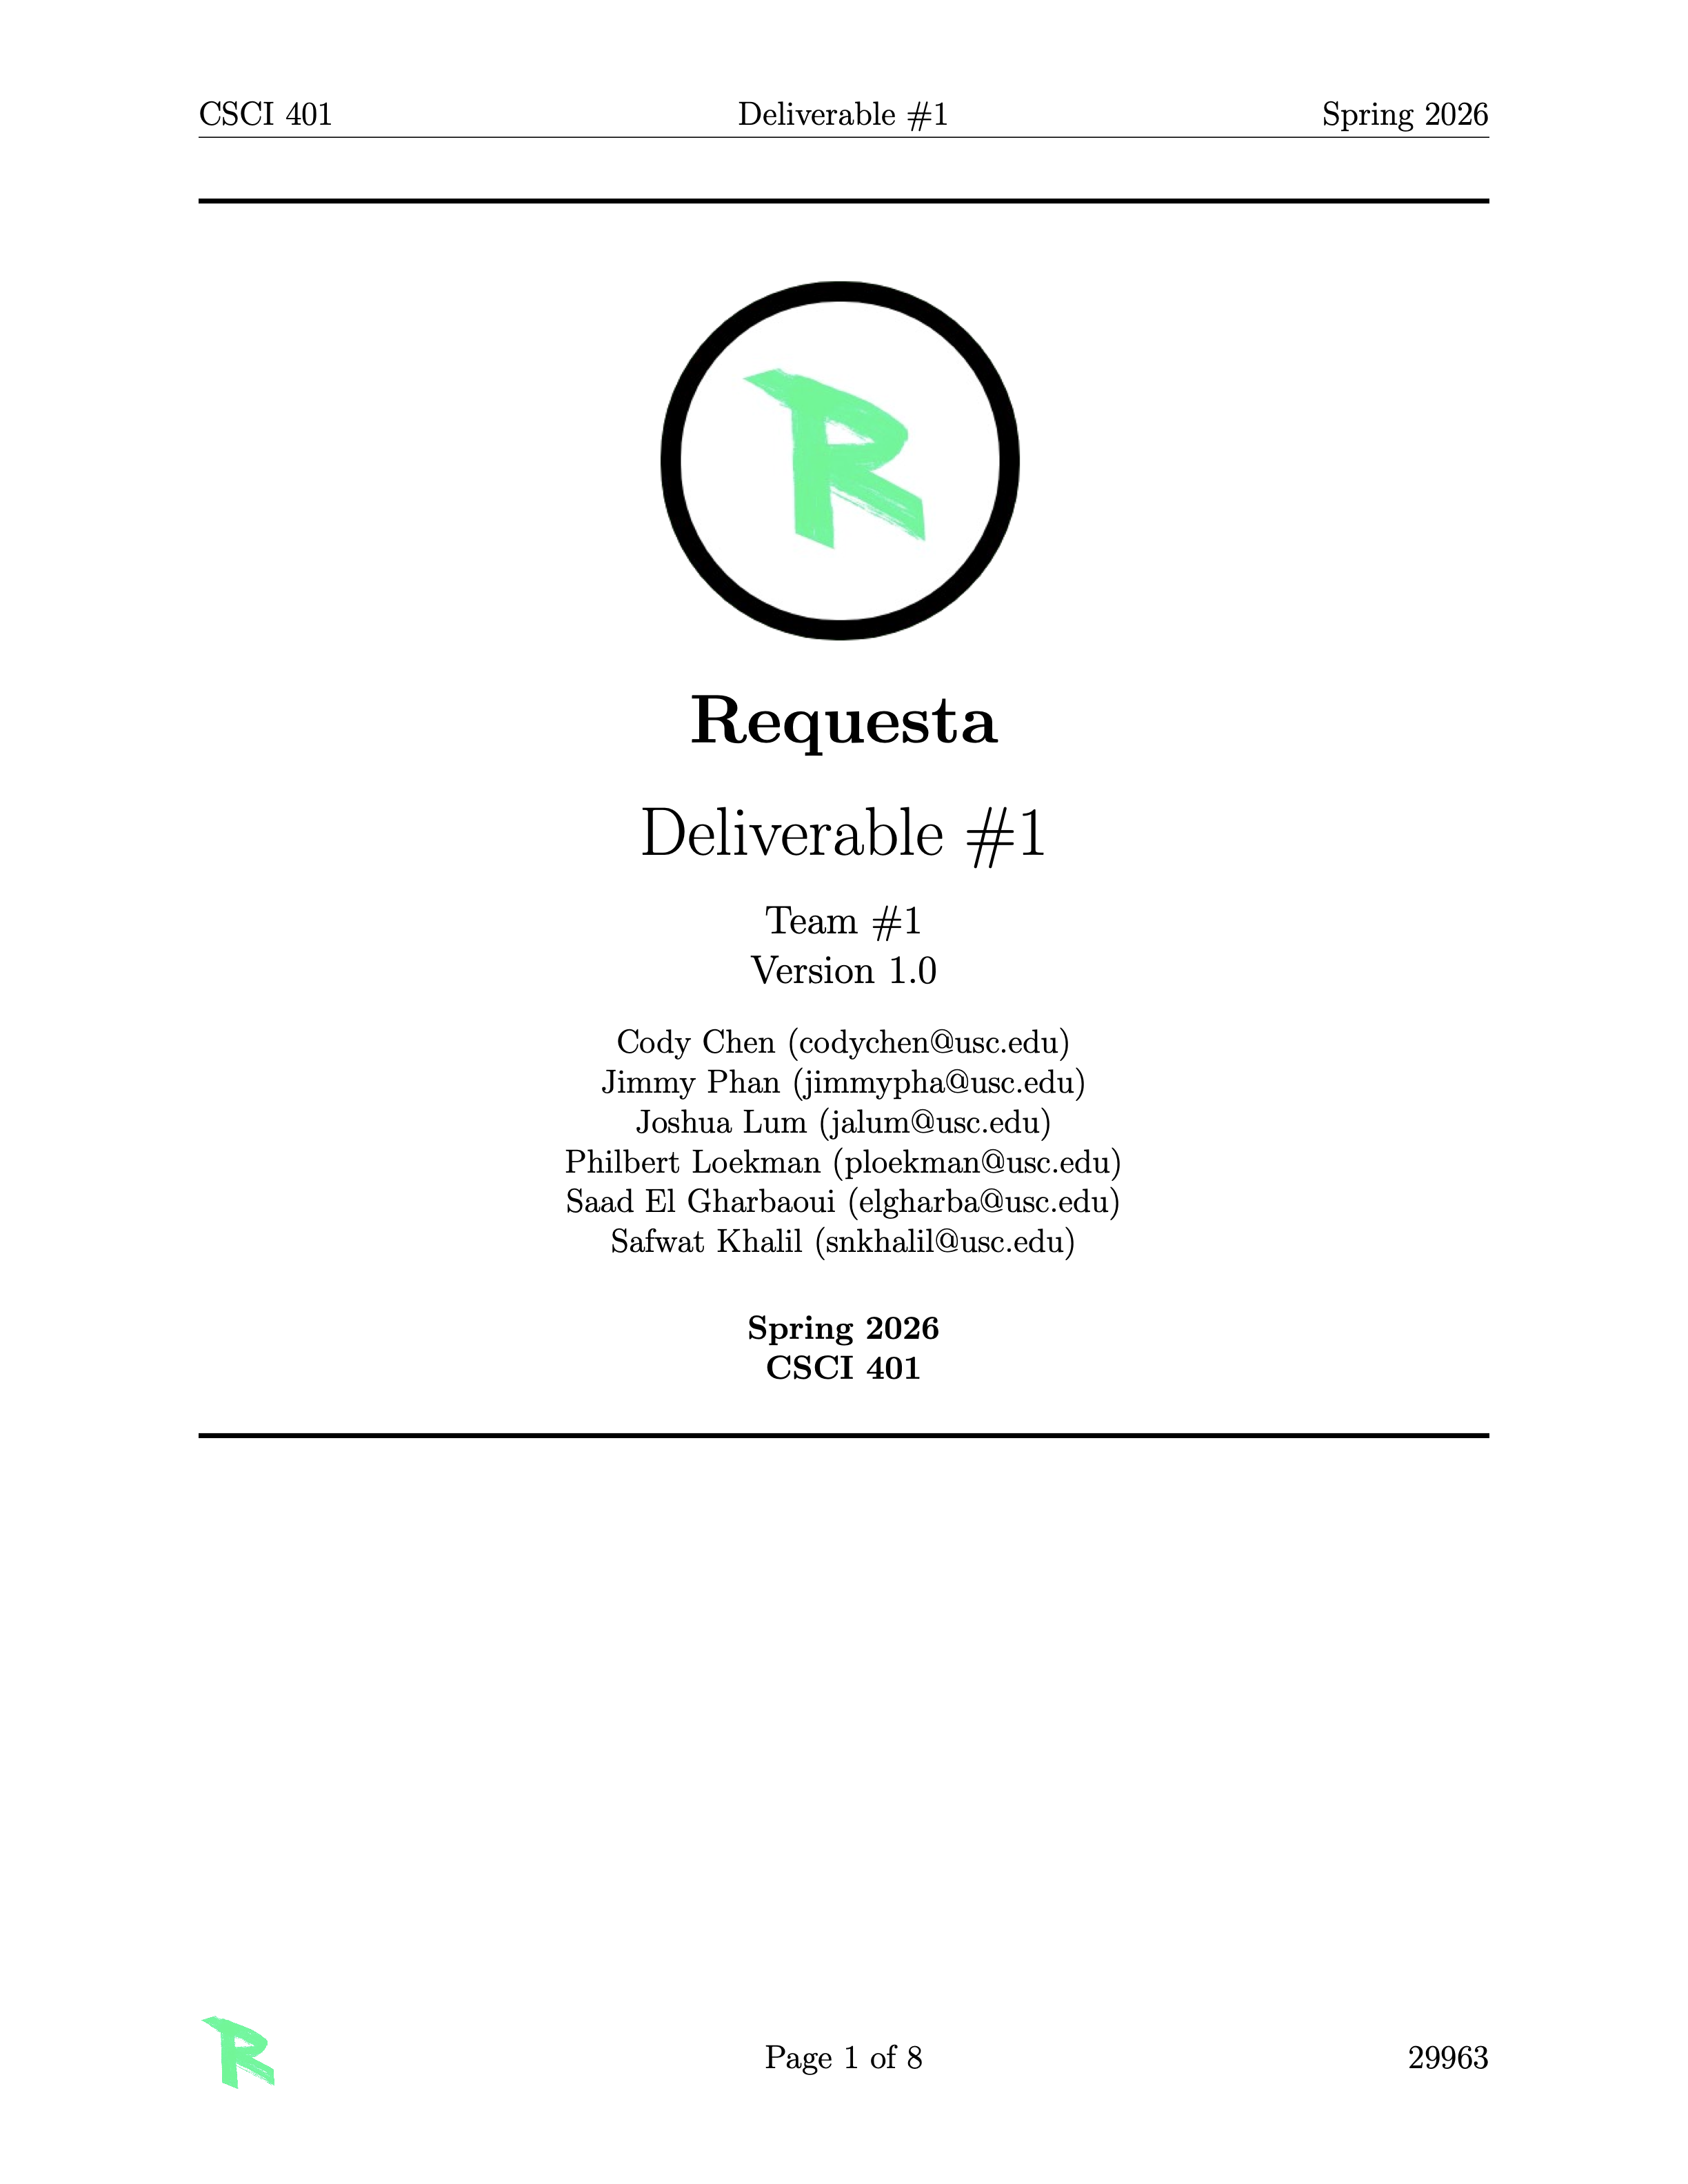
\includegraphics[width=0.48\textwidth,height=0.44\textheight,keepaspectratio]{images/deliverables/deliverable-1/Deliverable 1_1.png} &
            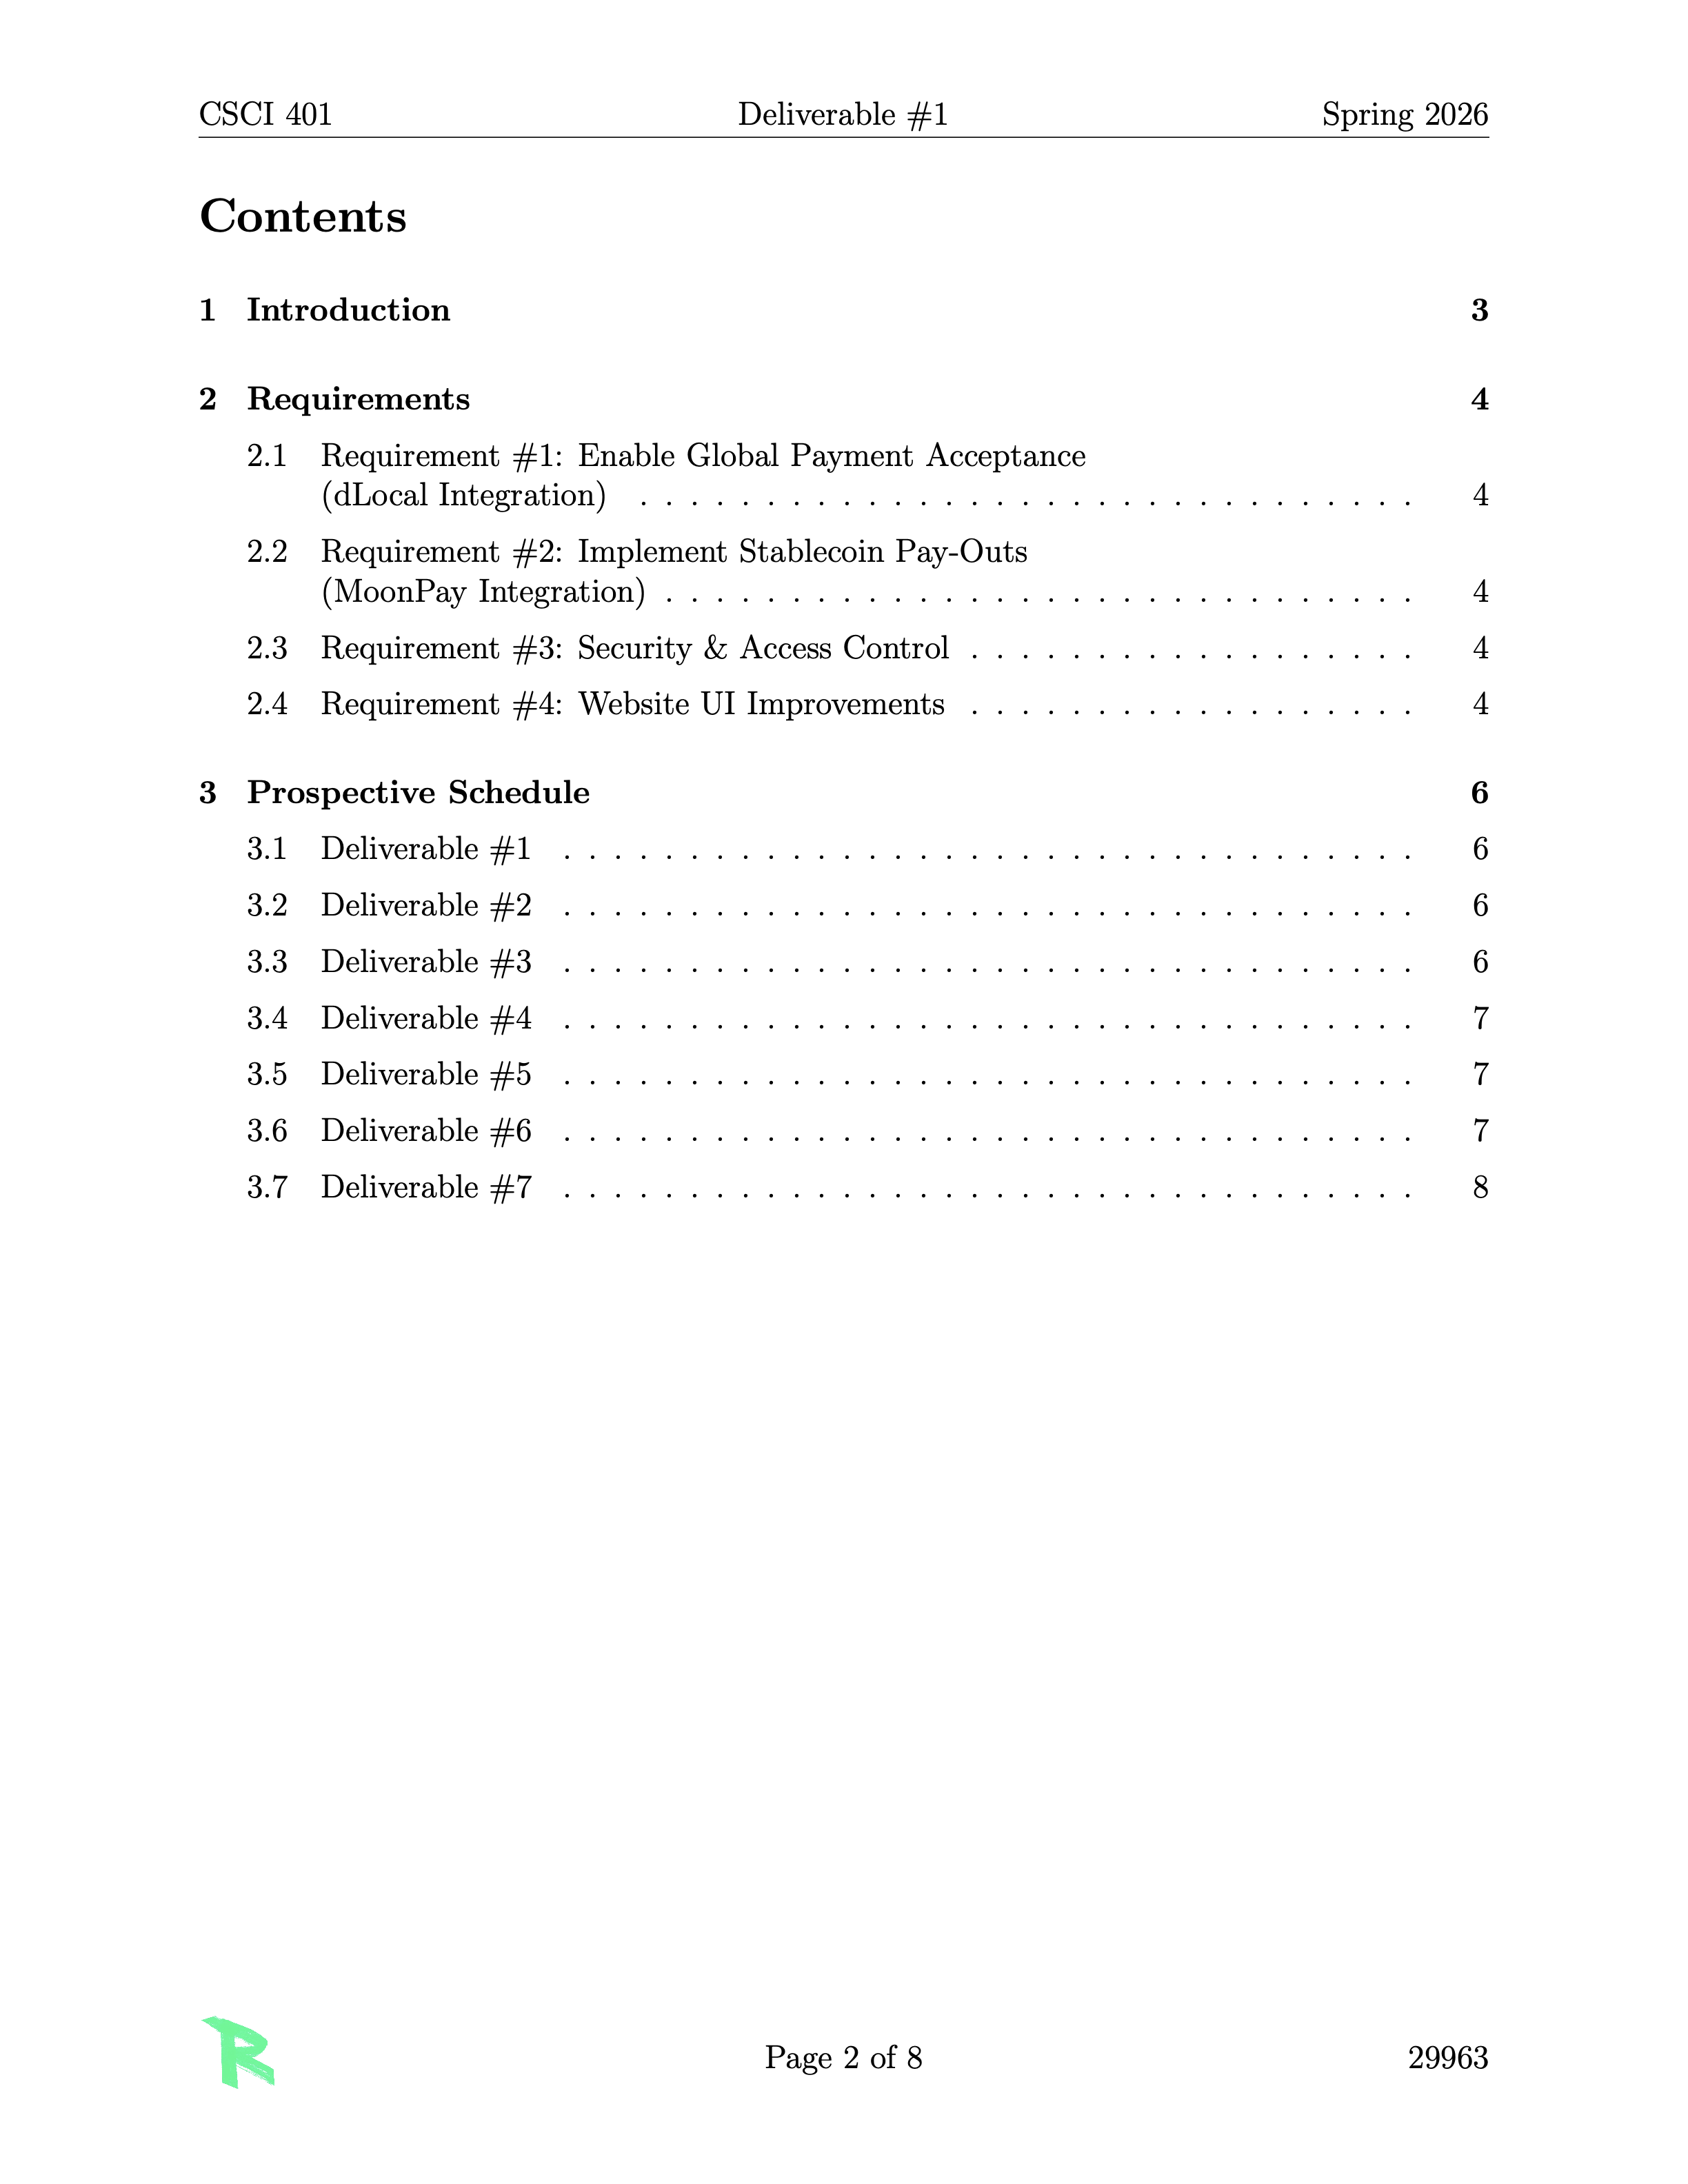
\includegraphics[width=0.48\textwidth,height=0.44\textheight,keepaspectratio]{images/deliverables/deliverable-1/Deliverable 1_2.png} \\[4pt]
            
\includegraphics[width=0.48\textwidth,height=0.44\textheight,keepaspectratio]{images/deliverables/deliverable-1/Deliverable 1_3.png} &
            
\includegraphics[width=0.48\textwidth,height=0.44\textheight,keepaspectratio]{images/deliverables/deliverable-1/Deliverable 1_4.png}
            \end{tabular}\end{figure}\clearpage

            \begin{figure}[H]\centering\setlength{\tabcolsep}{4pt}
            \begin{tabular}{cc}
            
\includegraphics[width=0.48\textwidth,height=0.44\textheight,keepaspectratio]{images/deliverables/deliverable-1/Deliverable 1_5.png} &
            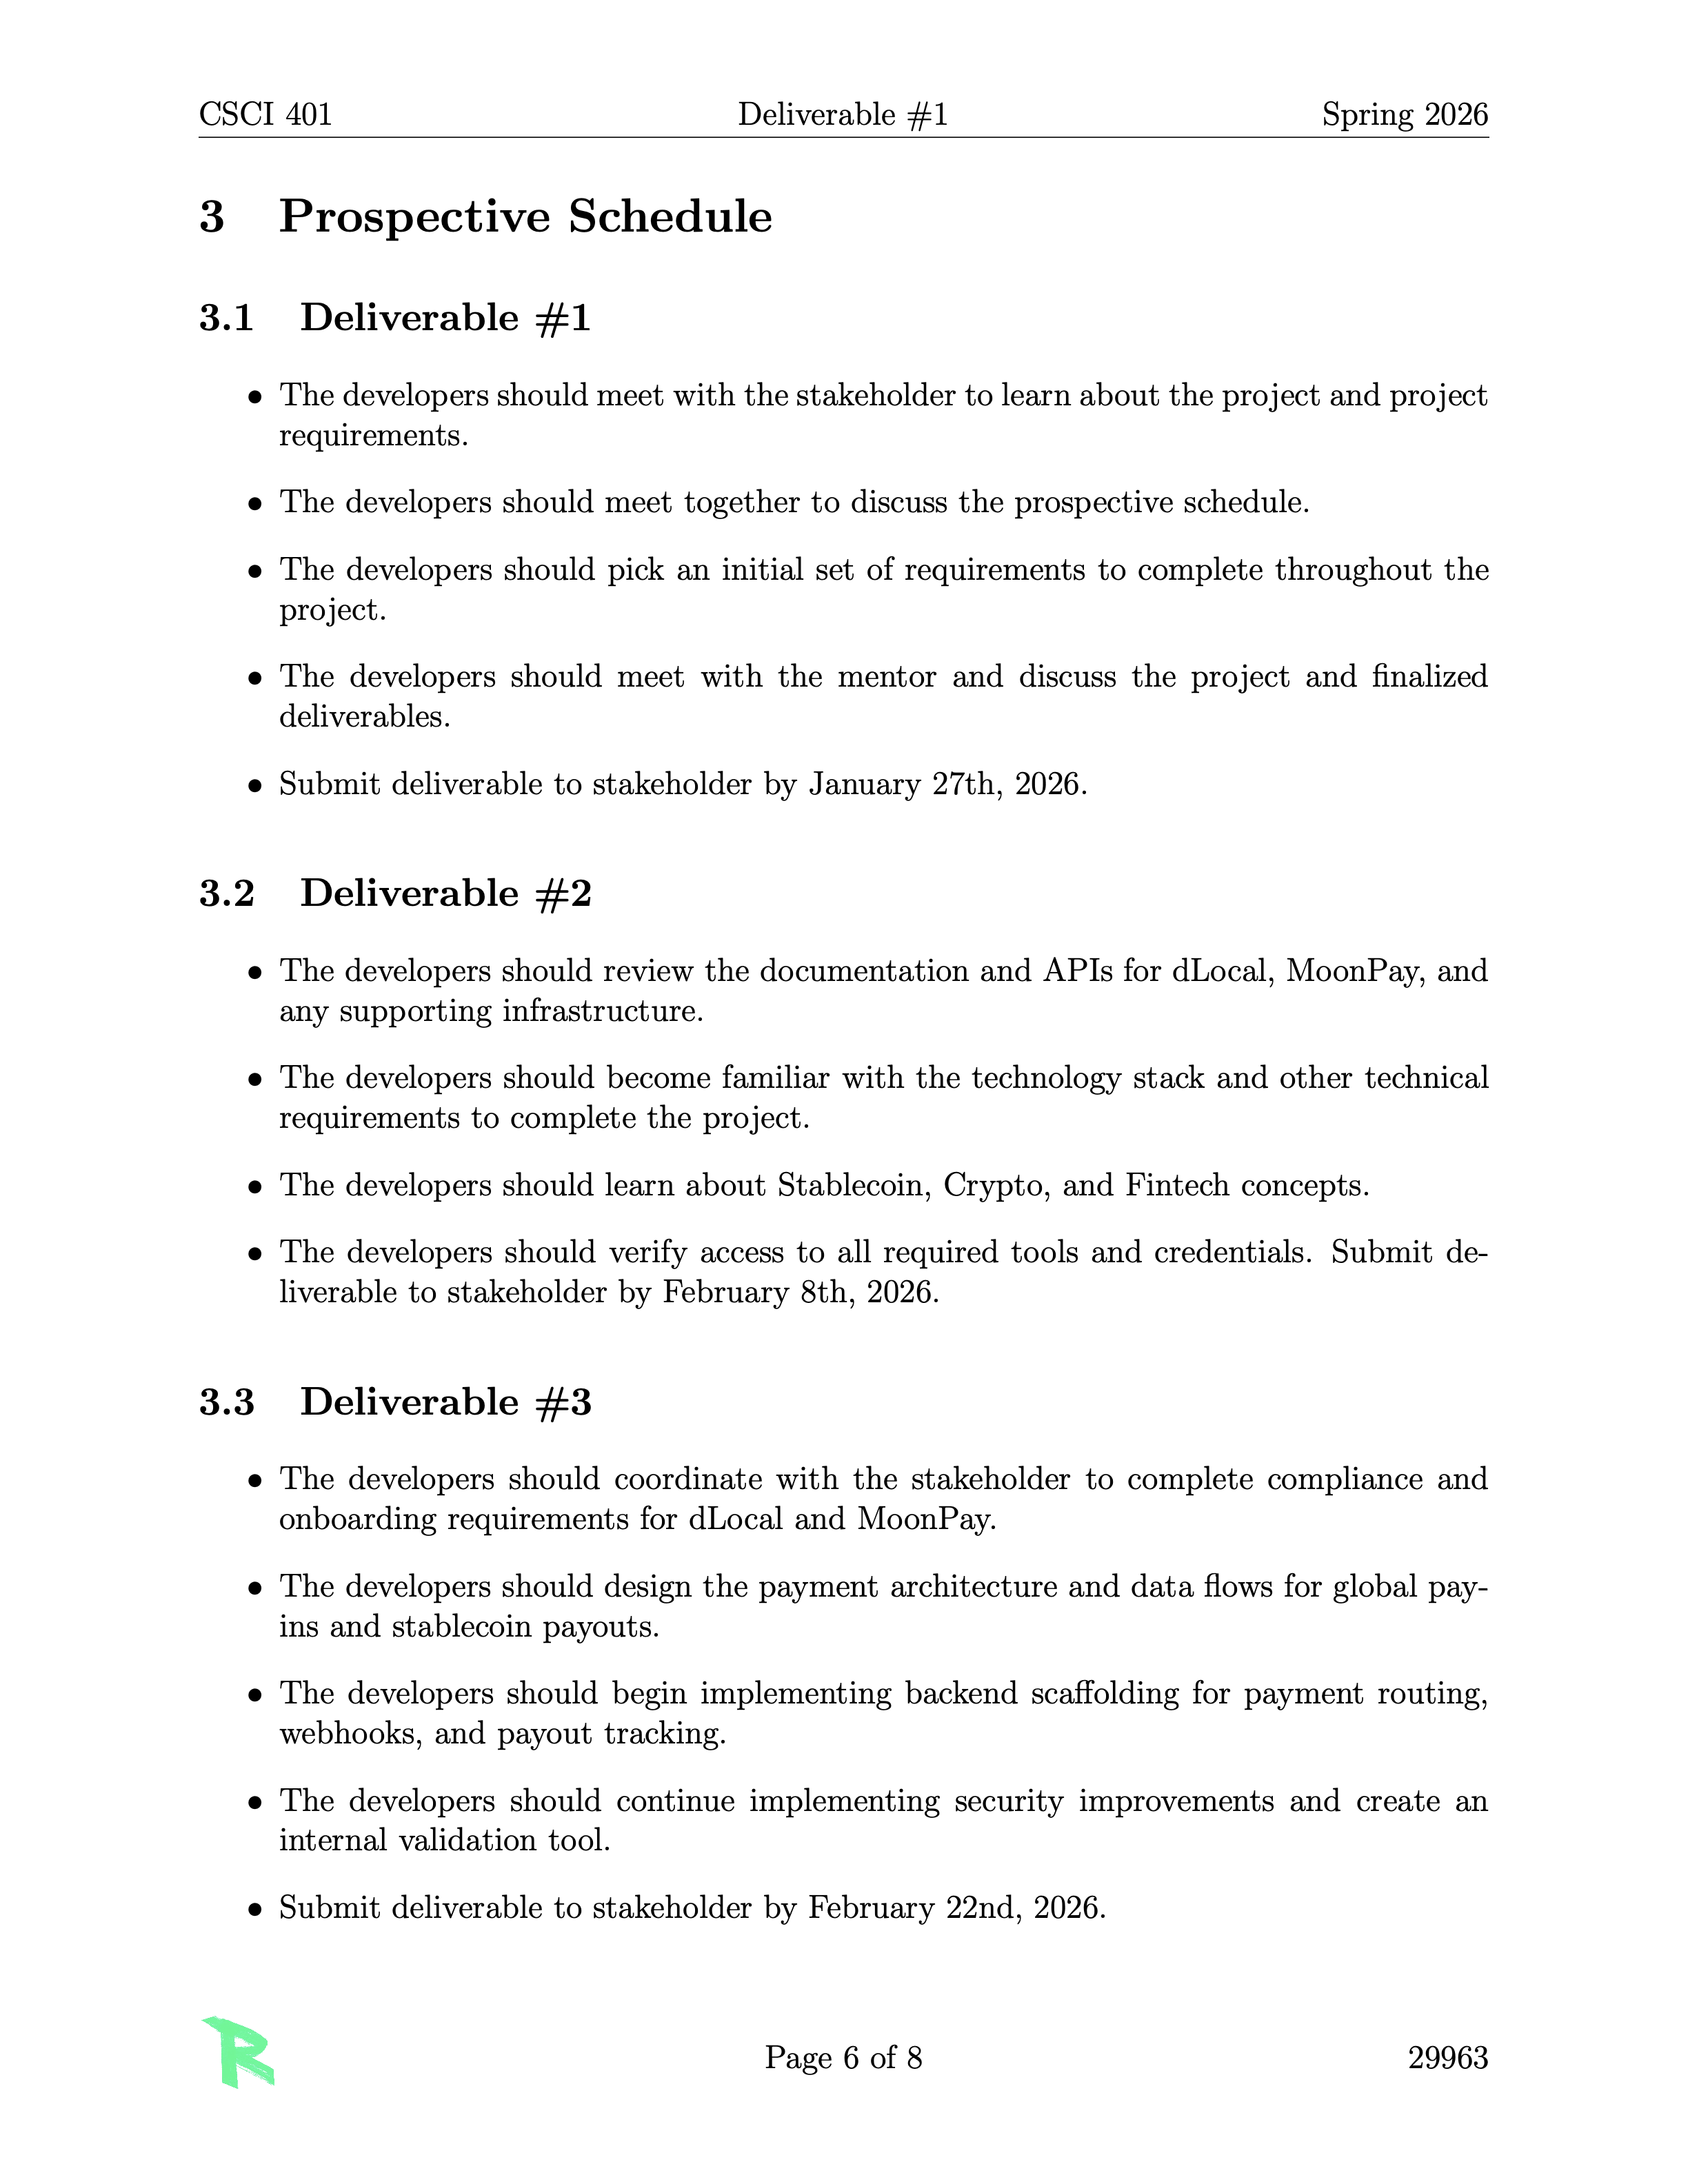
\includegraphics[width=0.48\textwidth,height=0.44\textheight,keepaspectratio]{images/deliverables/deliverable-1/Deliverable 1_6.png} \\[4pt]
            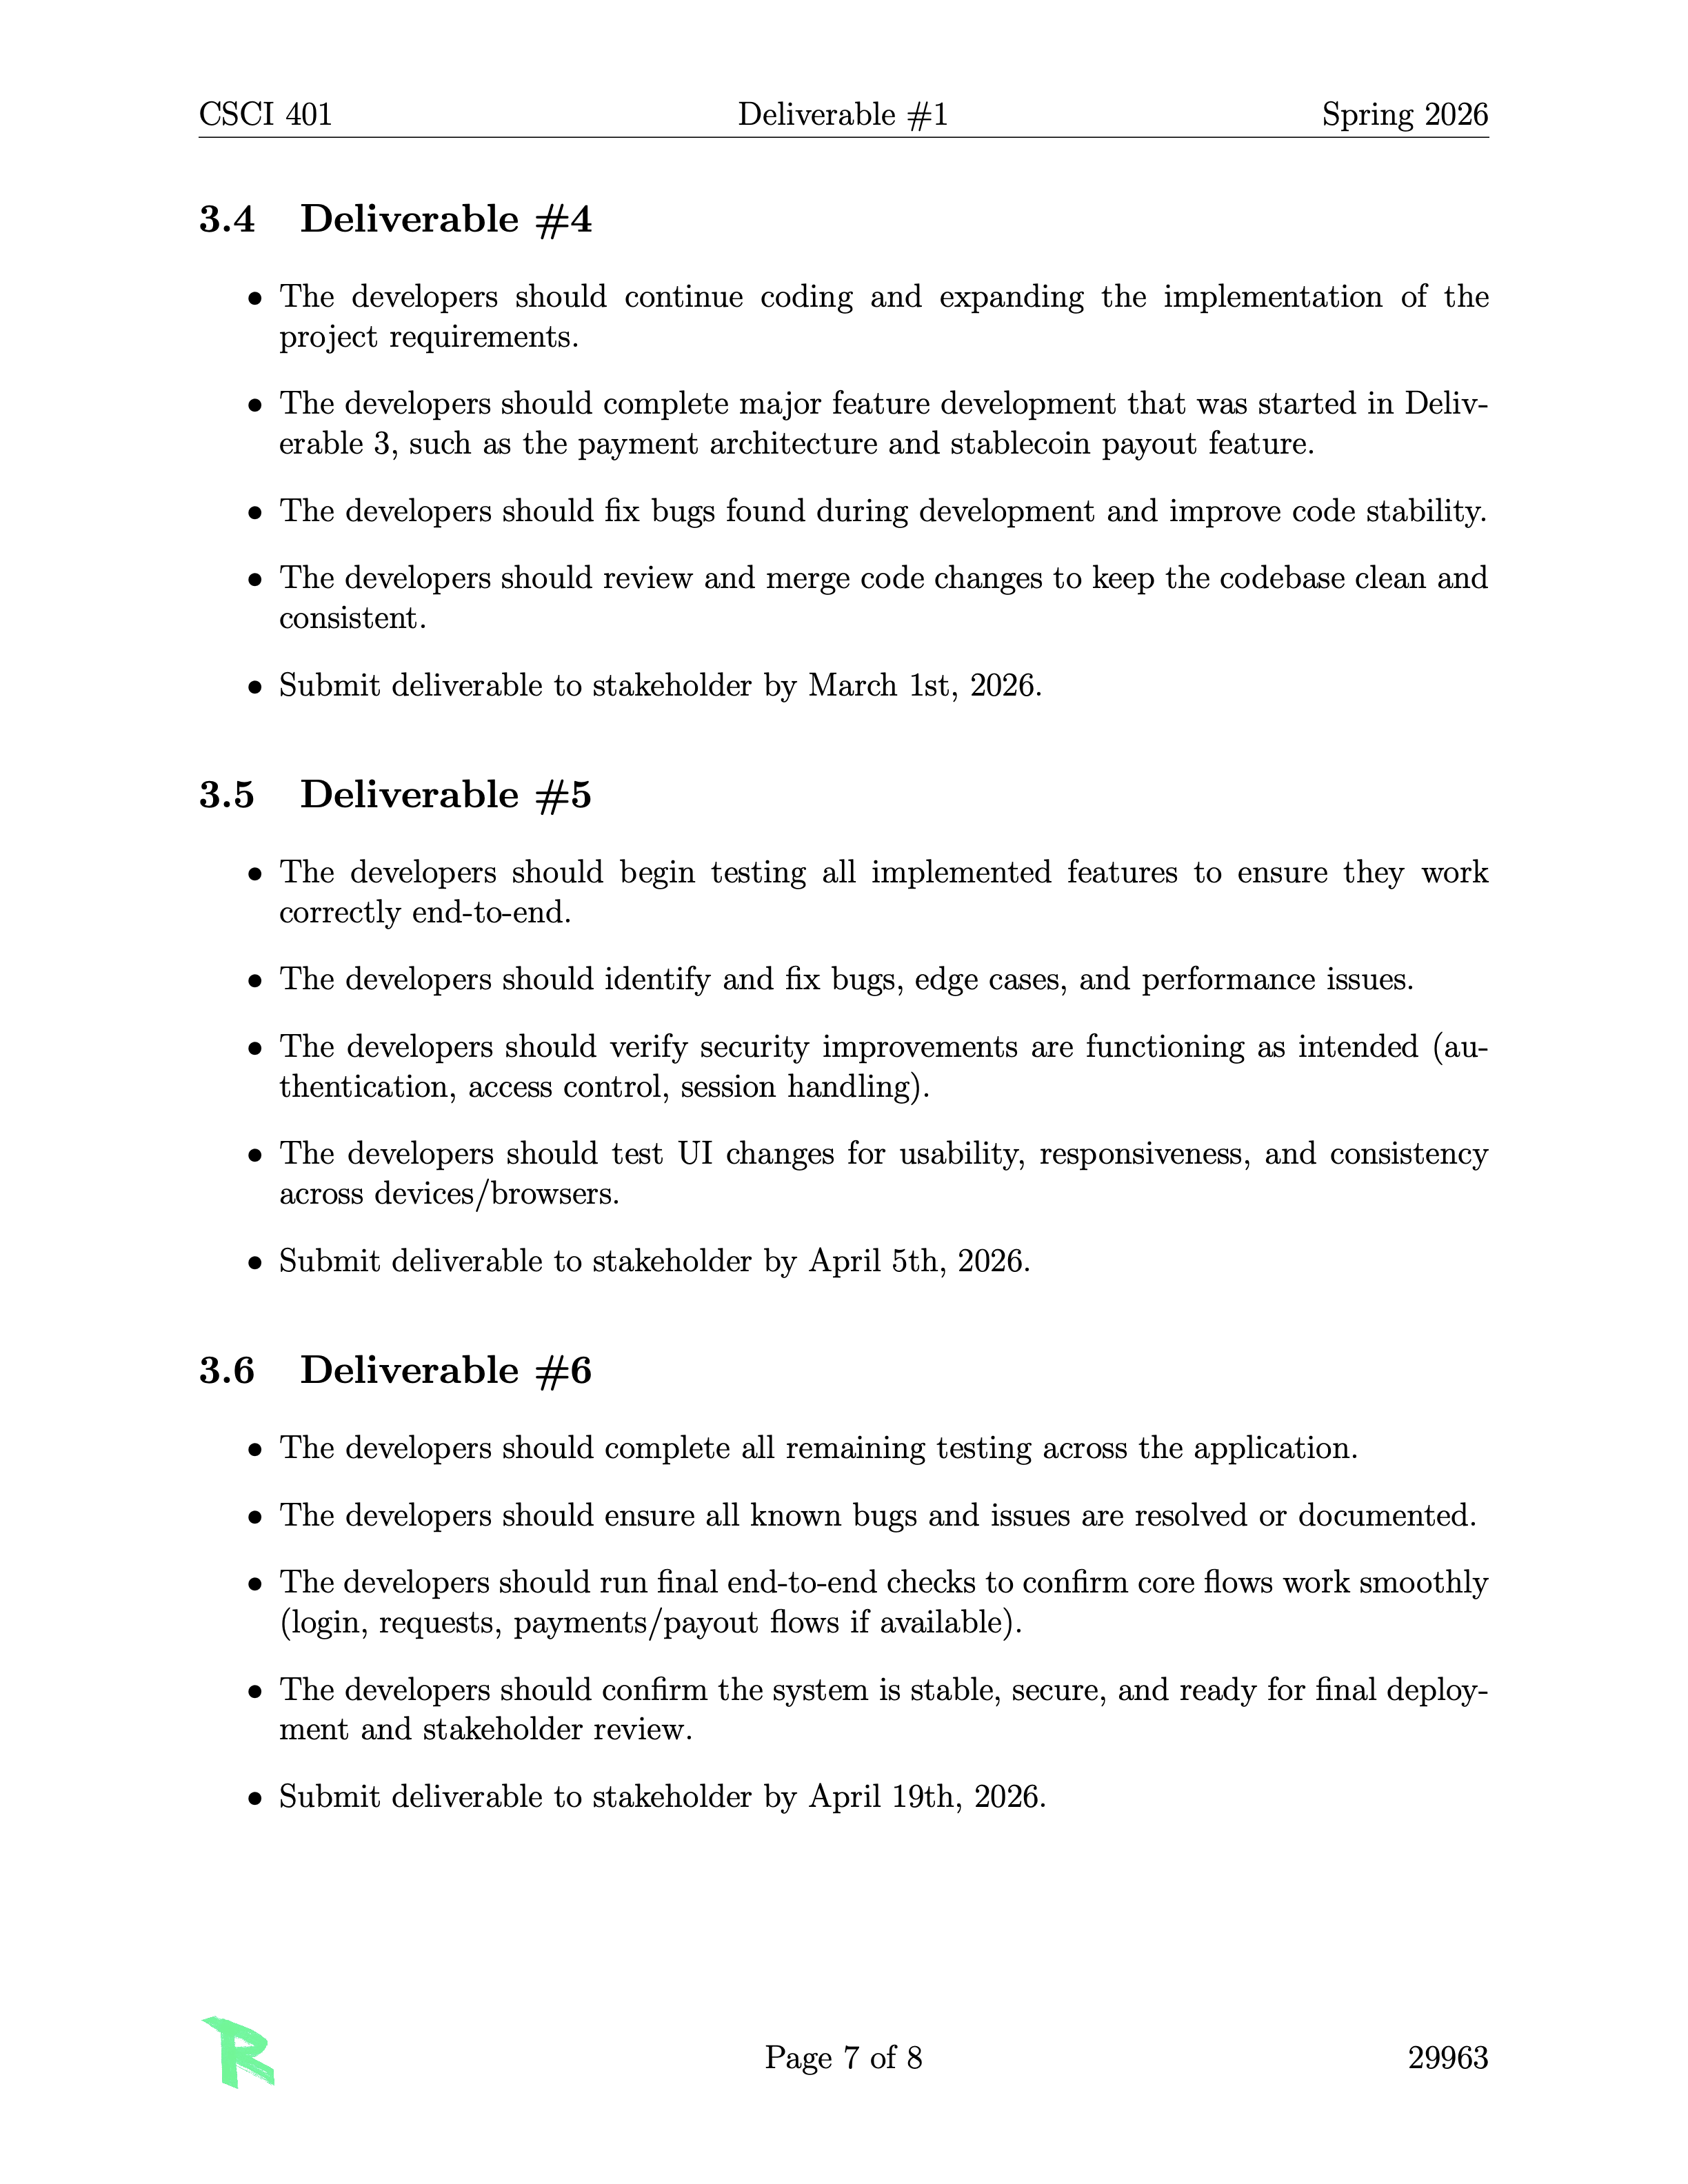
\includegraphics[width=0.48\textwidth,height=0.44\textheight,keepaspectratio]{images/deliverables/deliverable-1/Deliverable 1_7.png} &
            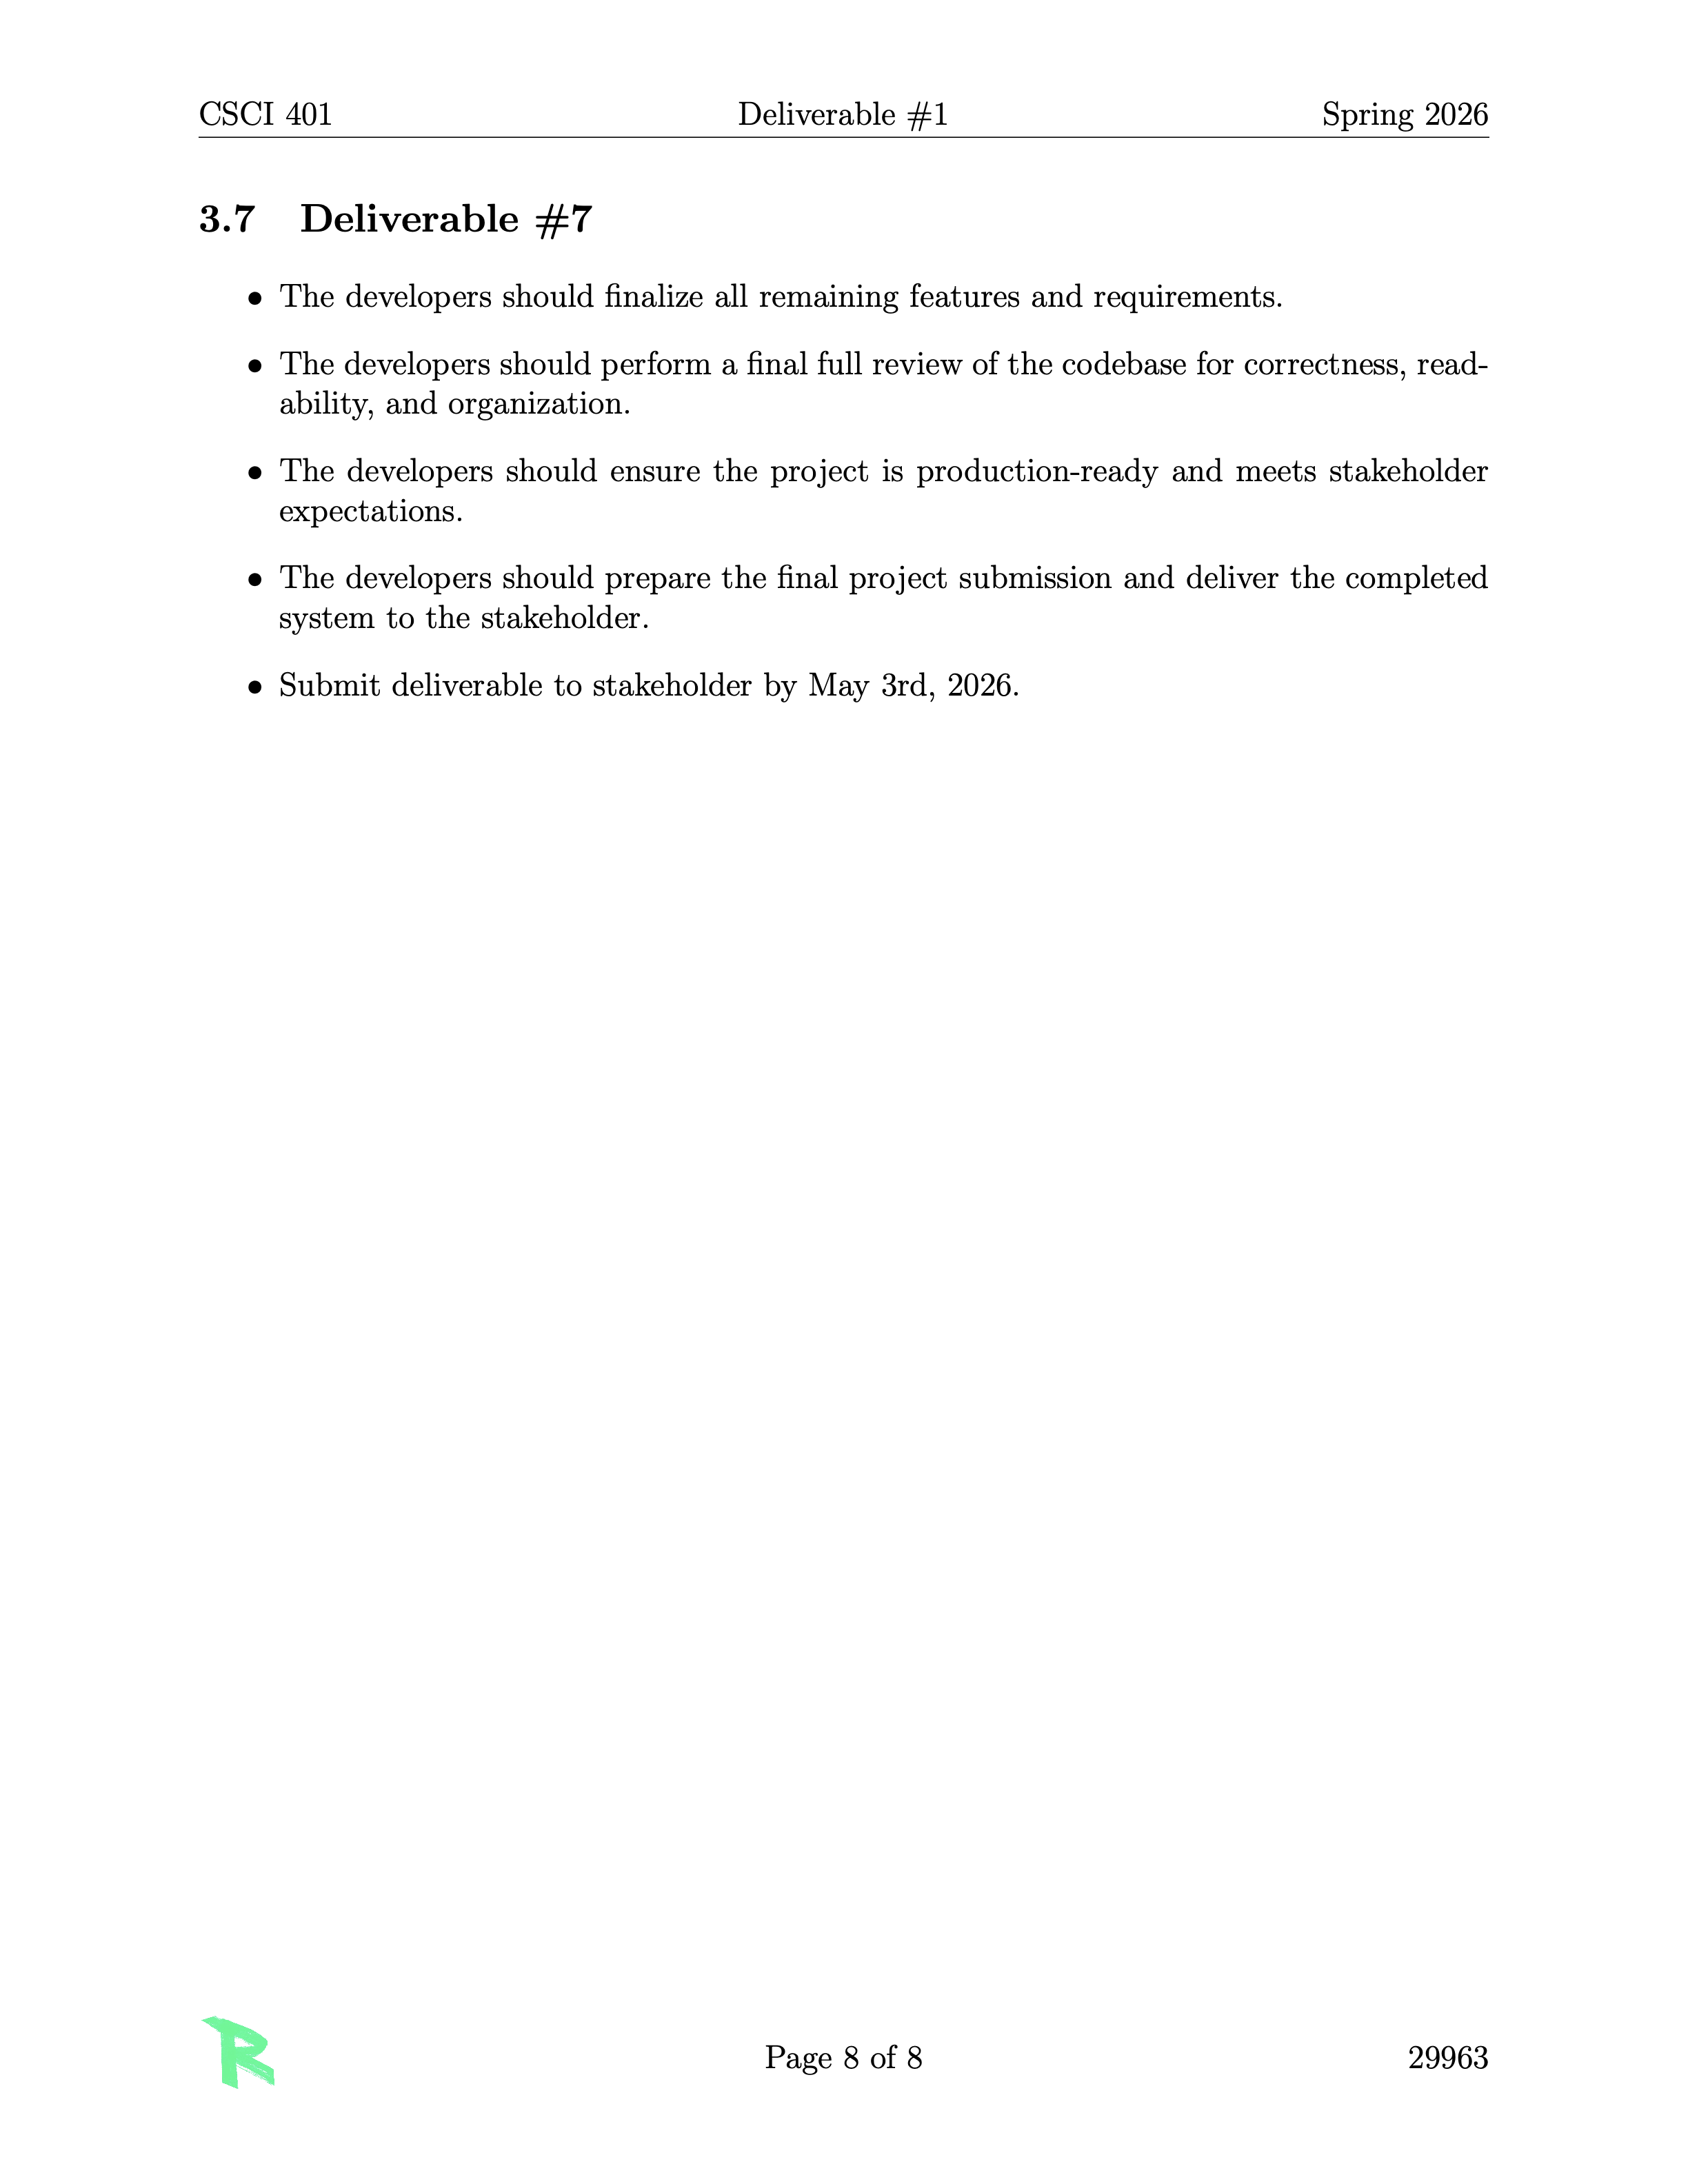
\includegraphics[width=0.48\textwidth,height=0.44\textheight,keepaspectratio]{images/deliverables/deliverable-1/Deliverable 1_8.png}
            \end{tabular}\end{figure}\clearpage

            \subsubsection{Deliverable 2}

            \begin{figure}[H]\centering\setlength{\tabcolsep}{4pt}
            \begin{tabular}{cc}
            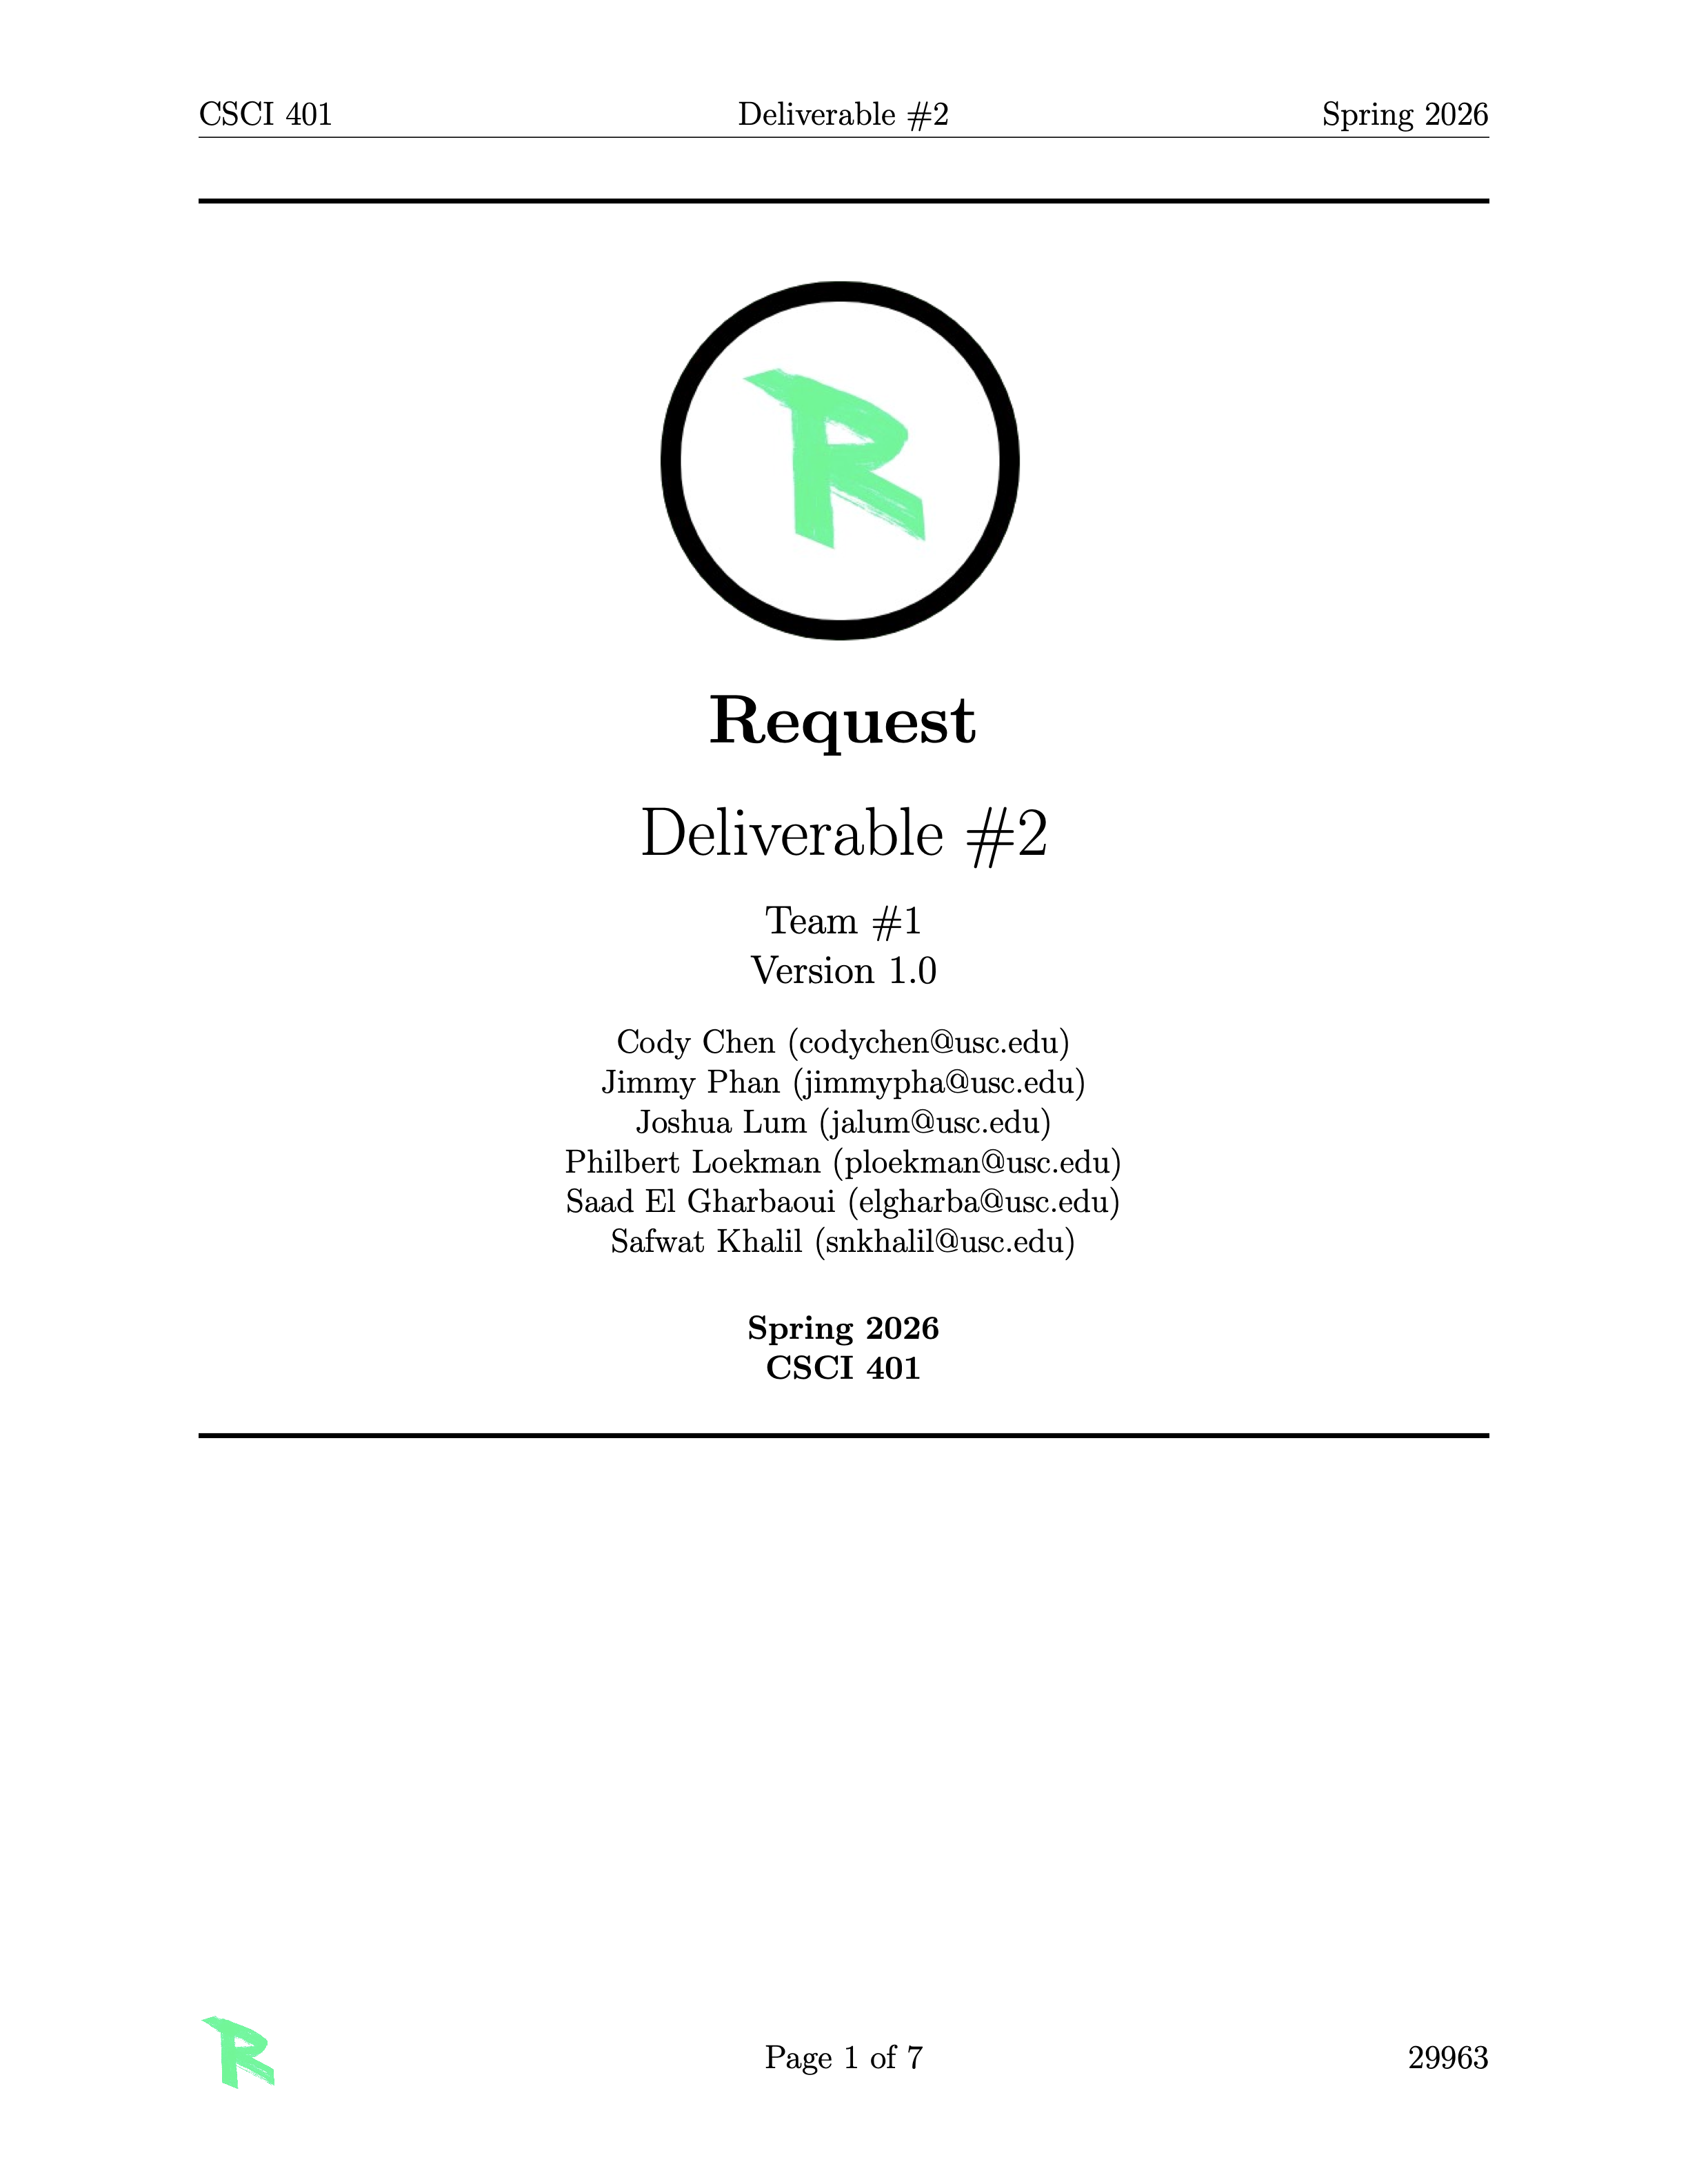
\includegraphics[width=0.48\textwidth,height=0.44\textheight,keepaspectratio]{images/deliverables/deliverable-2/Deliverable 2_1.png} &
            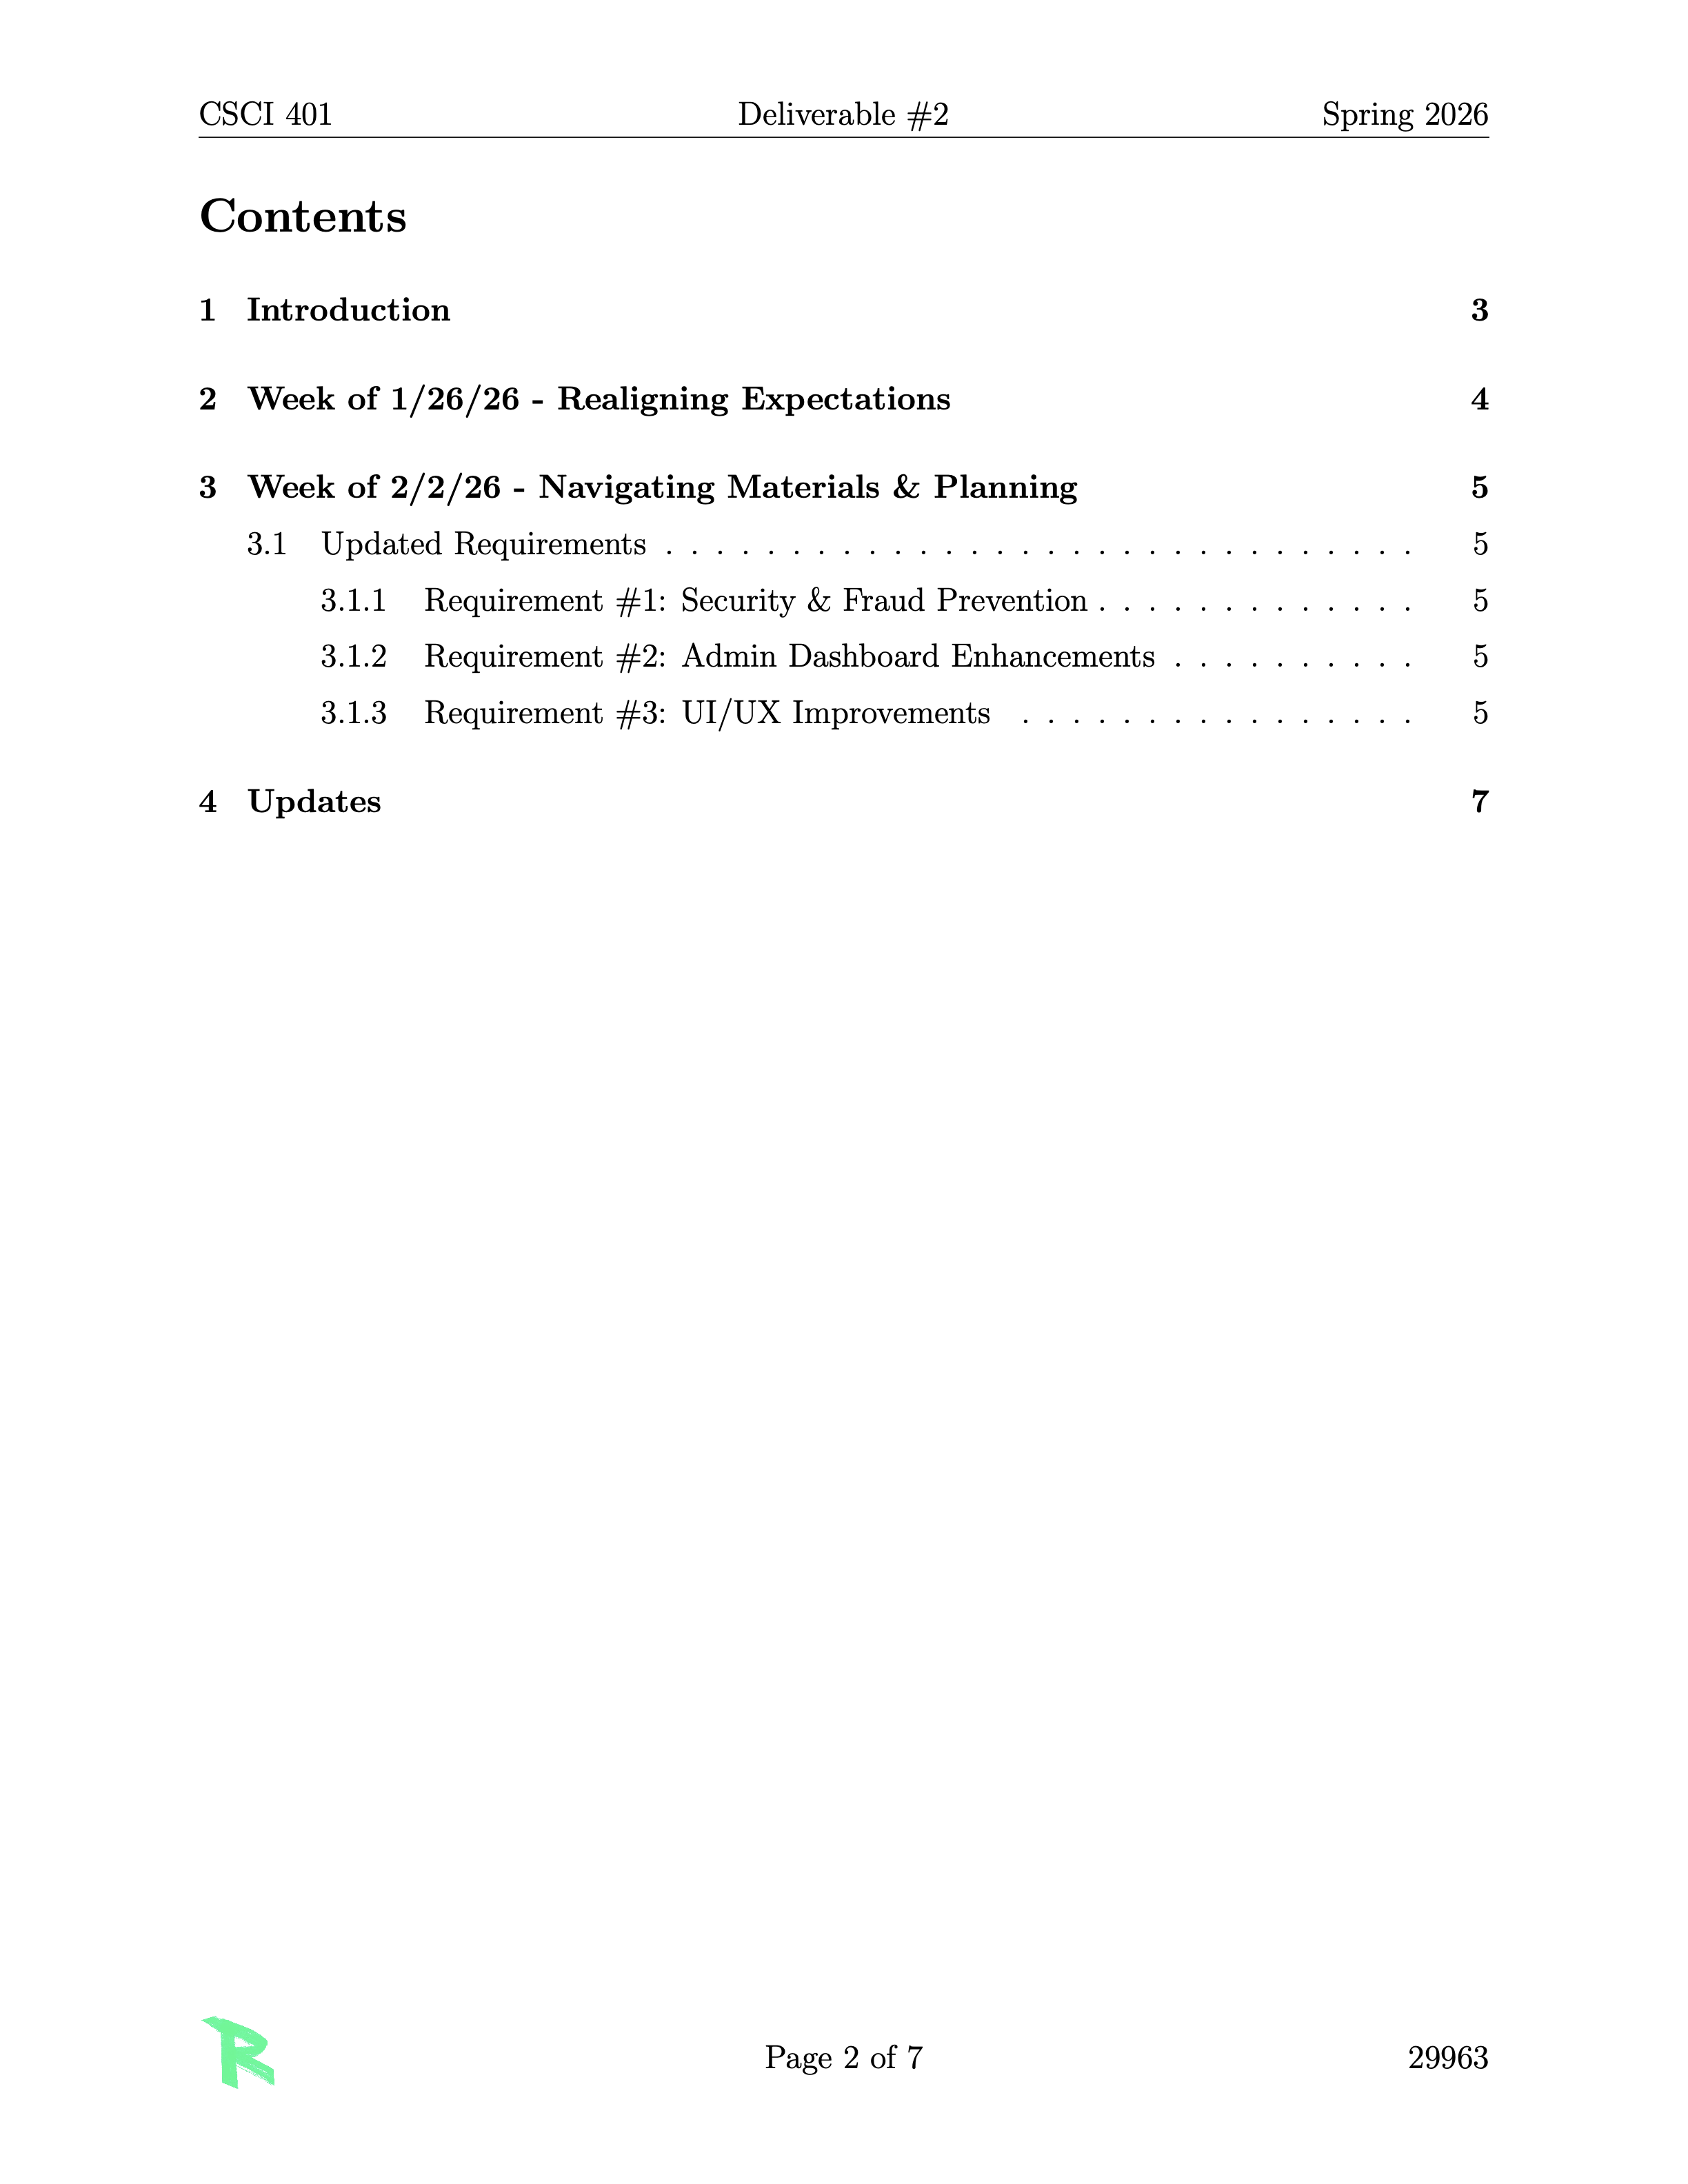
\includegraphics[width=0.48\textwidth,height=0.44\textheight,keepaspectratio]{images/deliverables/deliverable-2/Deliverable 2_2.png} \\[4pt]
            
\includegraphics[width=0.48\textwidth,height=0.44\textheight,keepaspectratio]{images/deliverables/deliverable-2/Deliverable 2_3.png} &
            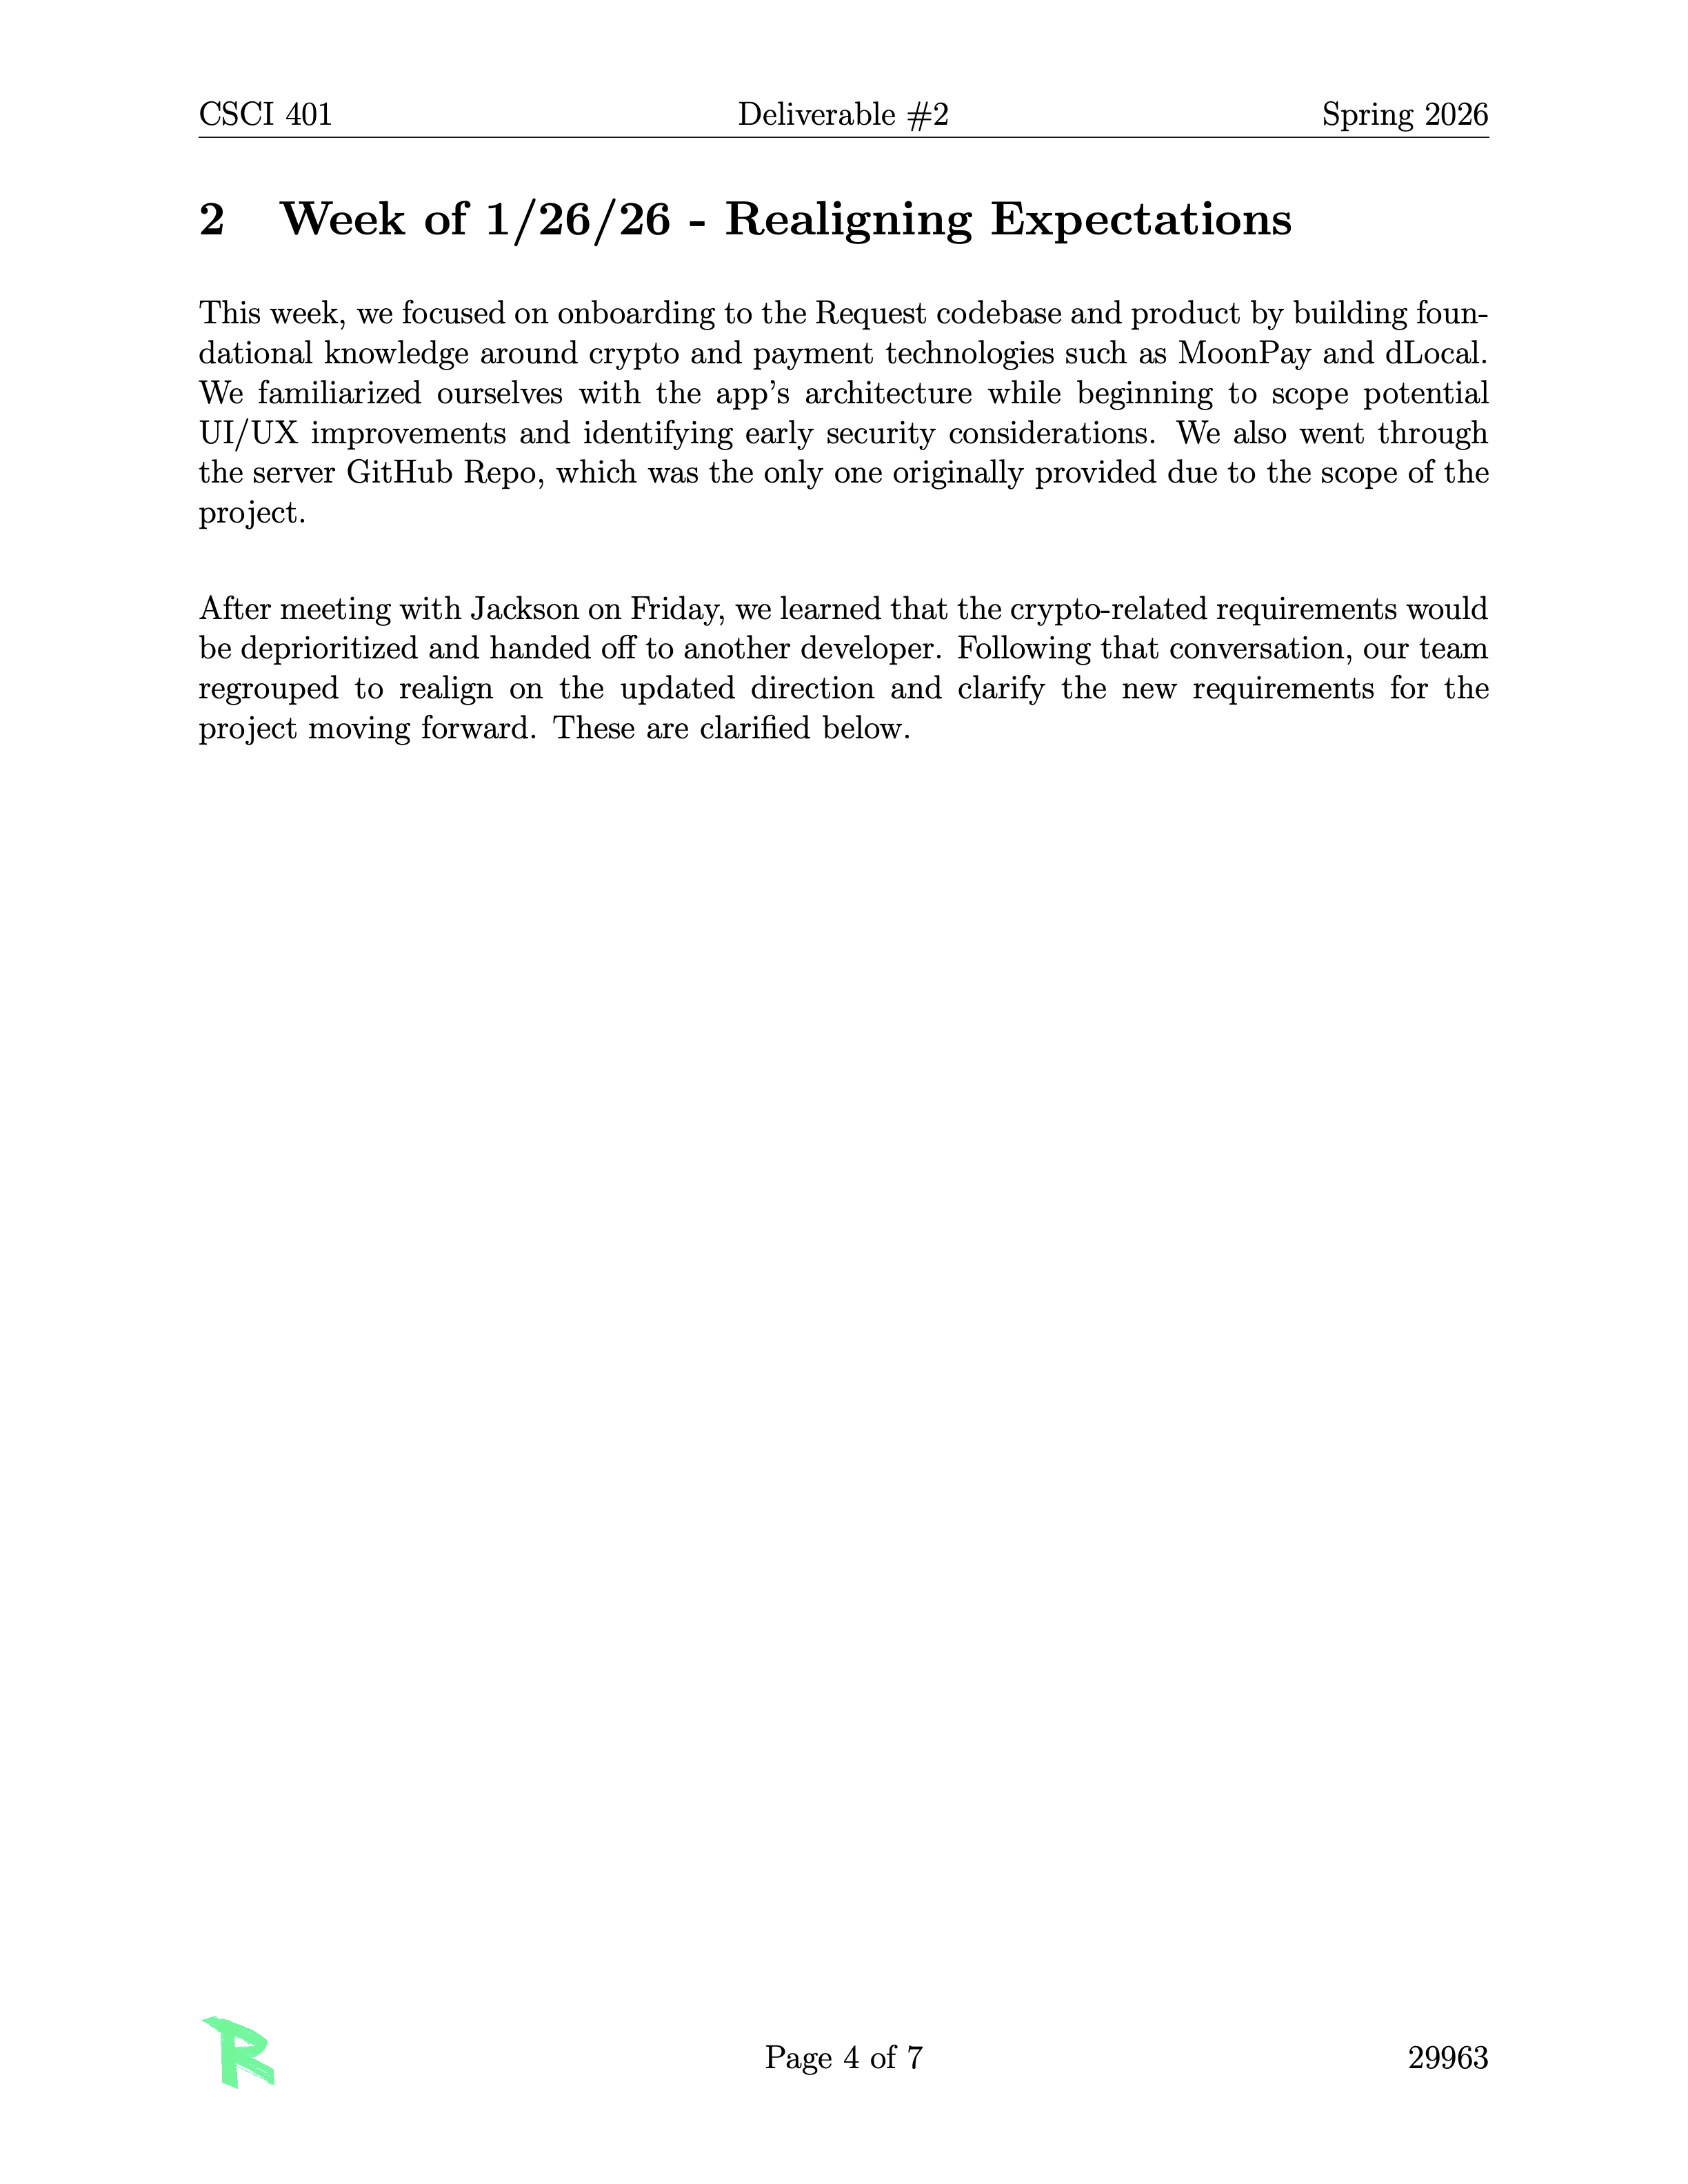
\includegraphics[width=0.48\textwidth,height=0.44\textheight,keepaspectratio]{images/deliverables/deliverable-2/Deliverable 2_4.png}
            \end{tabular}\end{figure}\clearpage

            \begin{figure}[H]\centering\setlength{\tabcolsep}{4pt}
            \begin{tabular}{cc}
            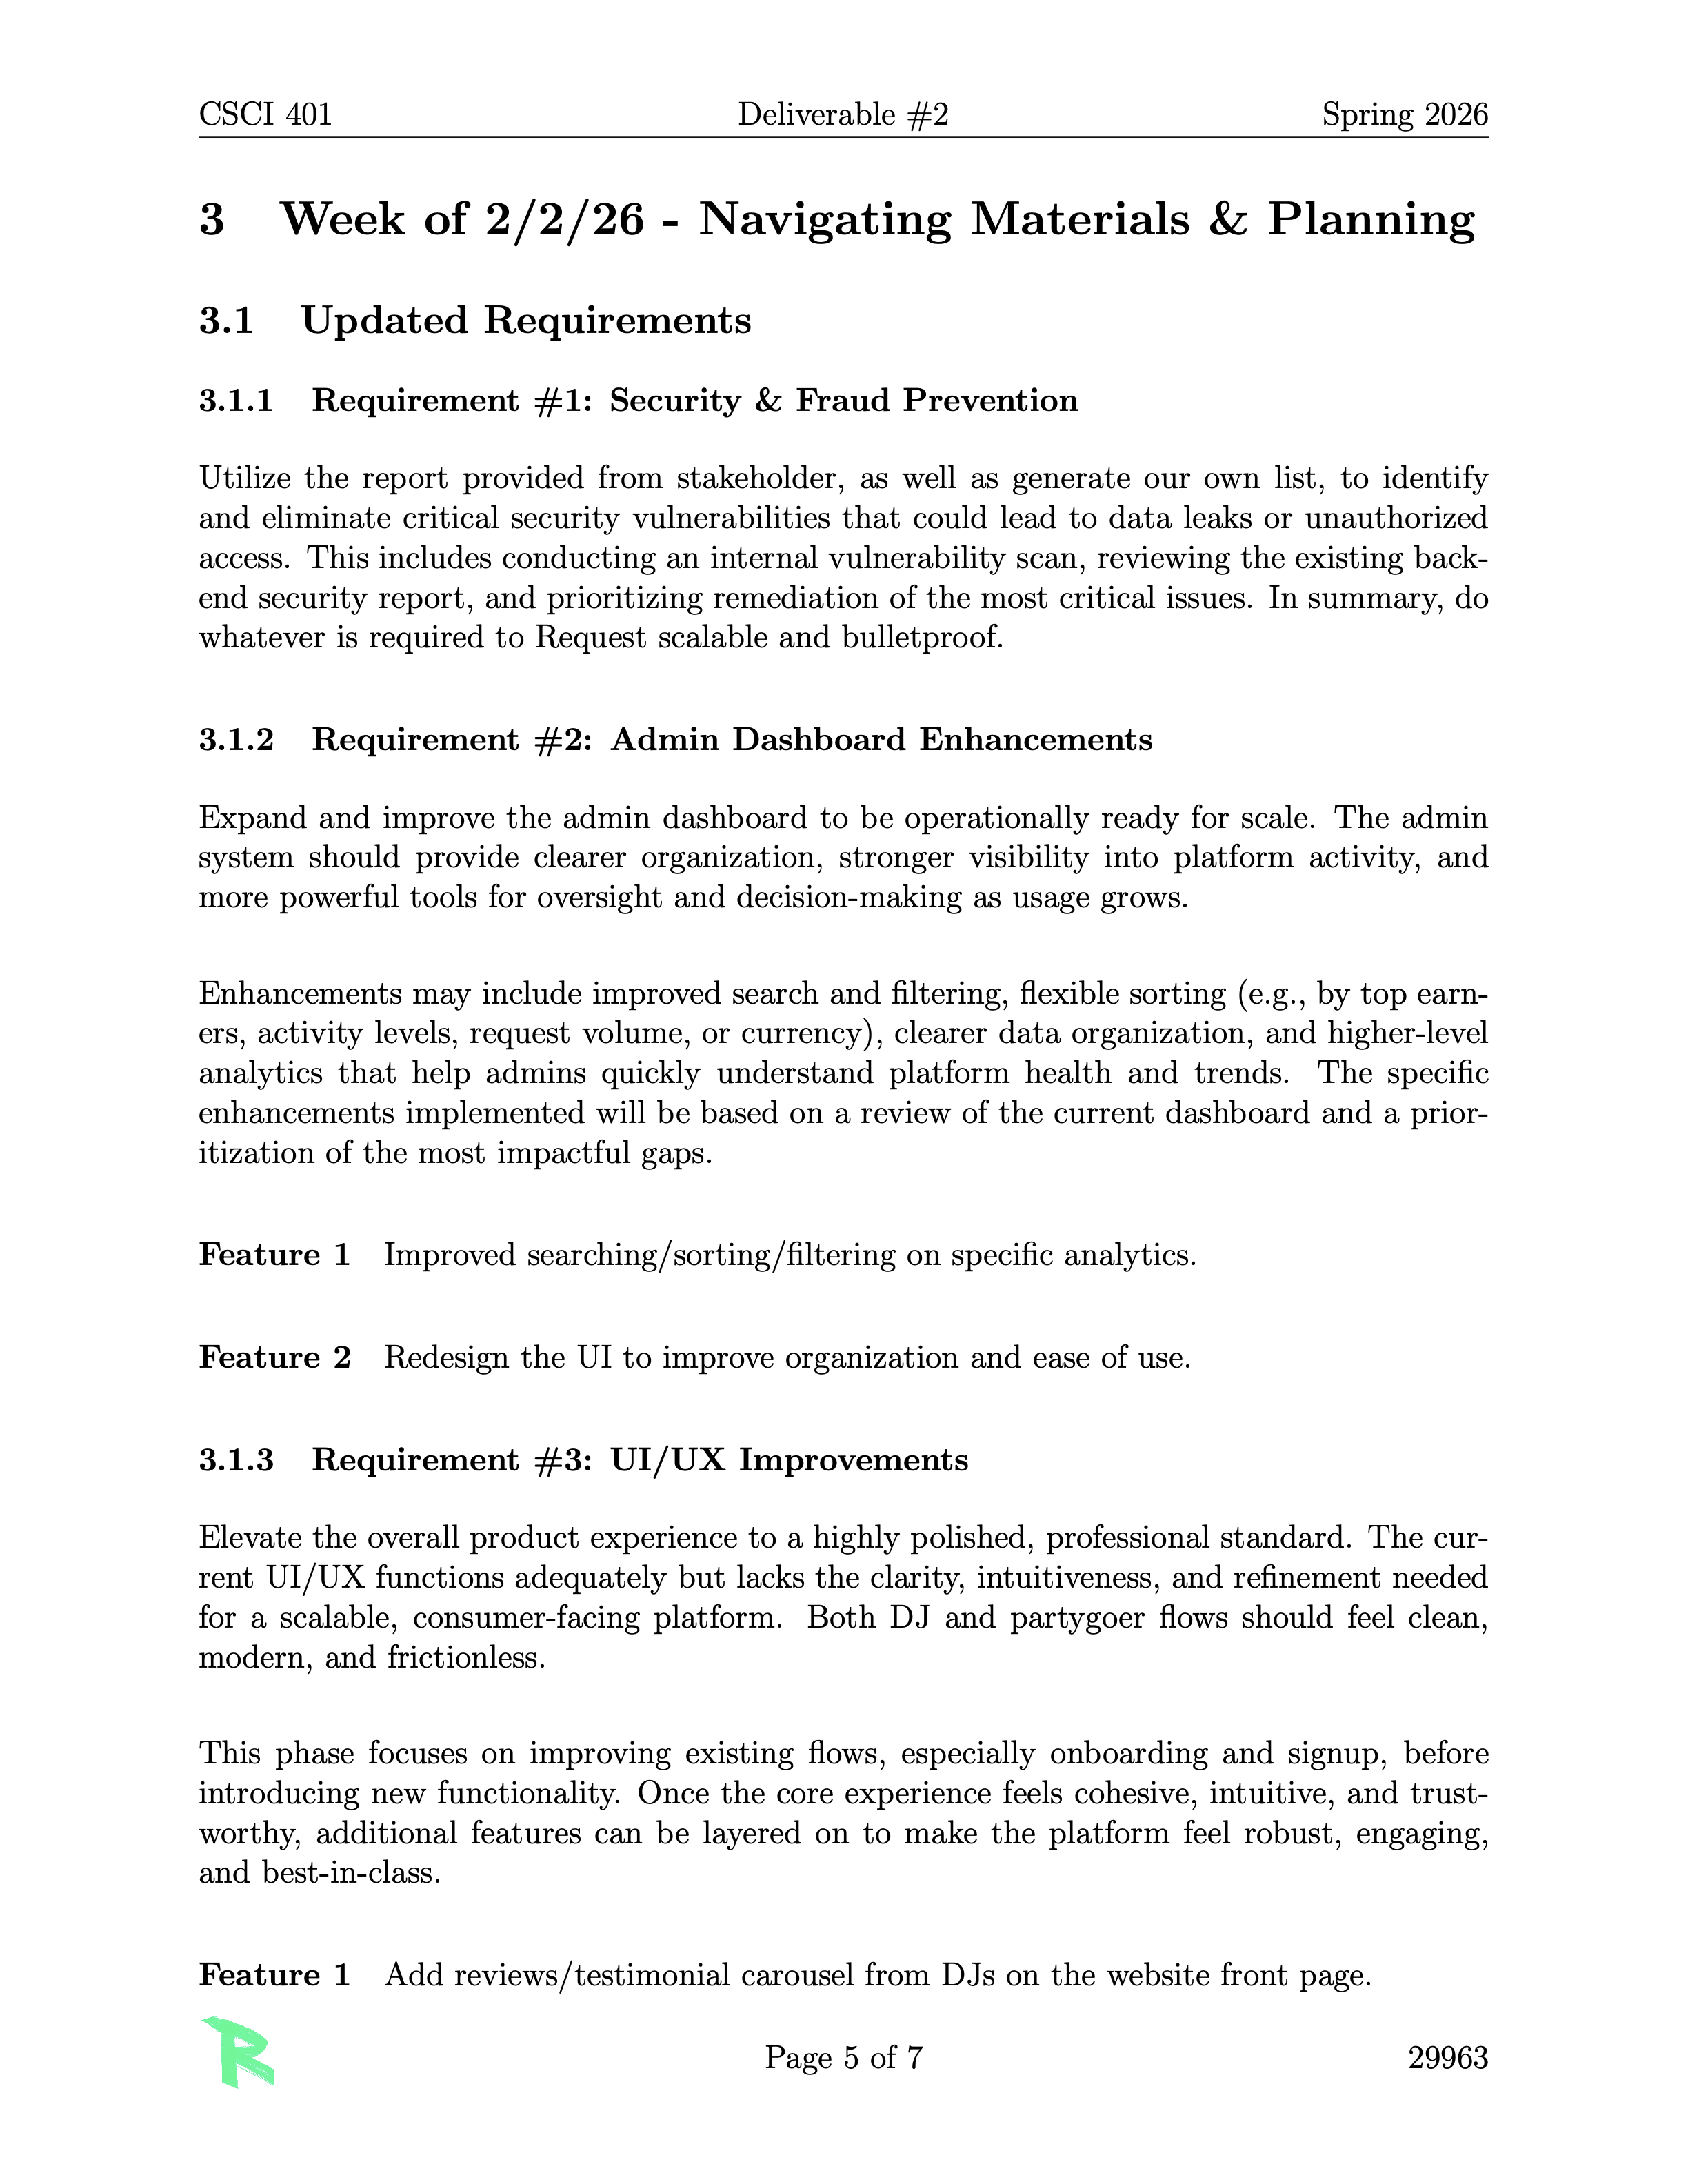
\includegraphics[width=0.48\textwidth,height=0.44\textheight,keepaspectratio]{images/deliverables/deliverable-2/Deliverable 2_5.png} &
            
\includegraphics[width=0.48\textwidth,height=0.44\textheight,keepaspectratio]{images/deliverables/deliverable-2/Deliverable 2_6.png} \\[4pt]
            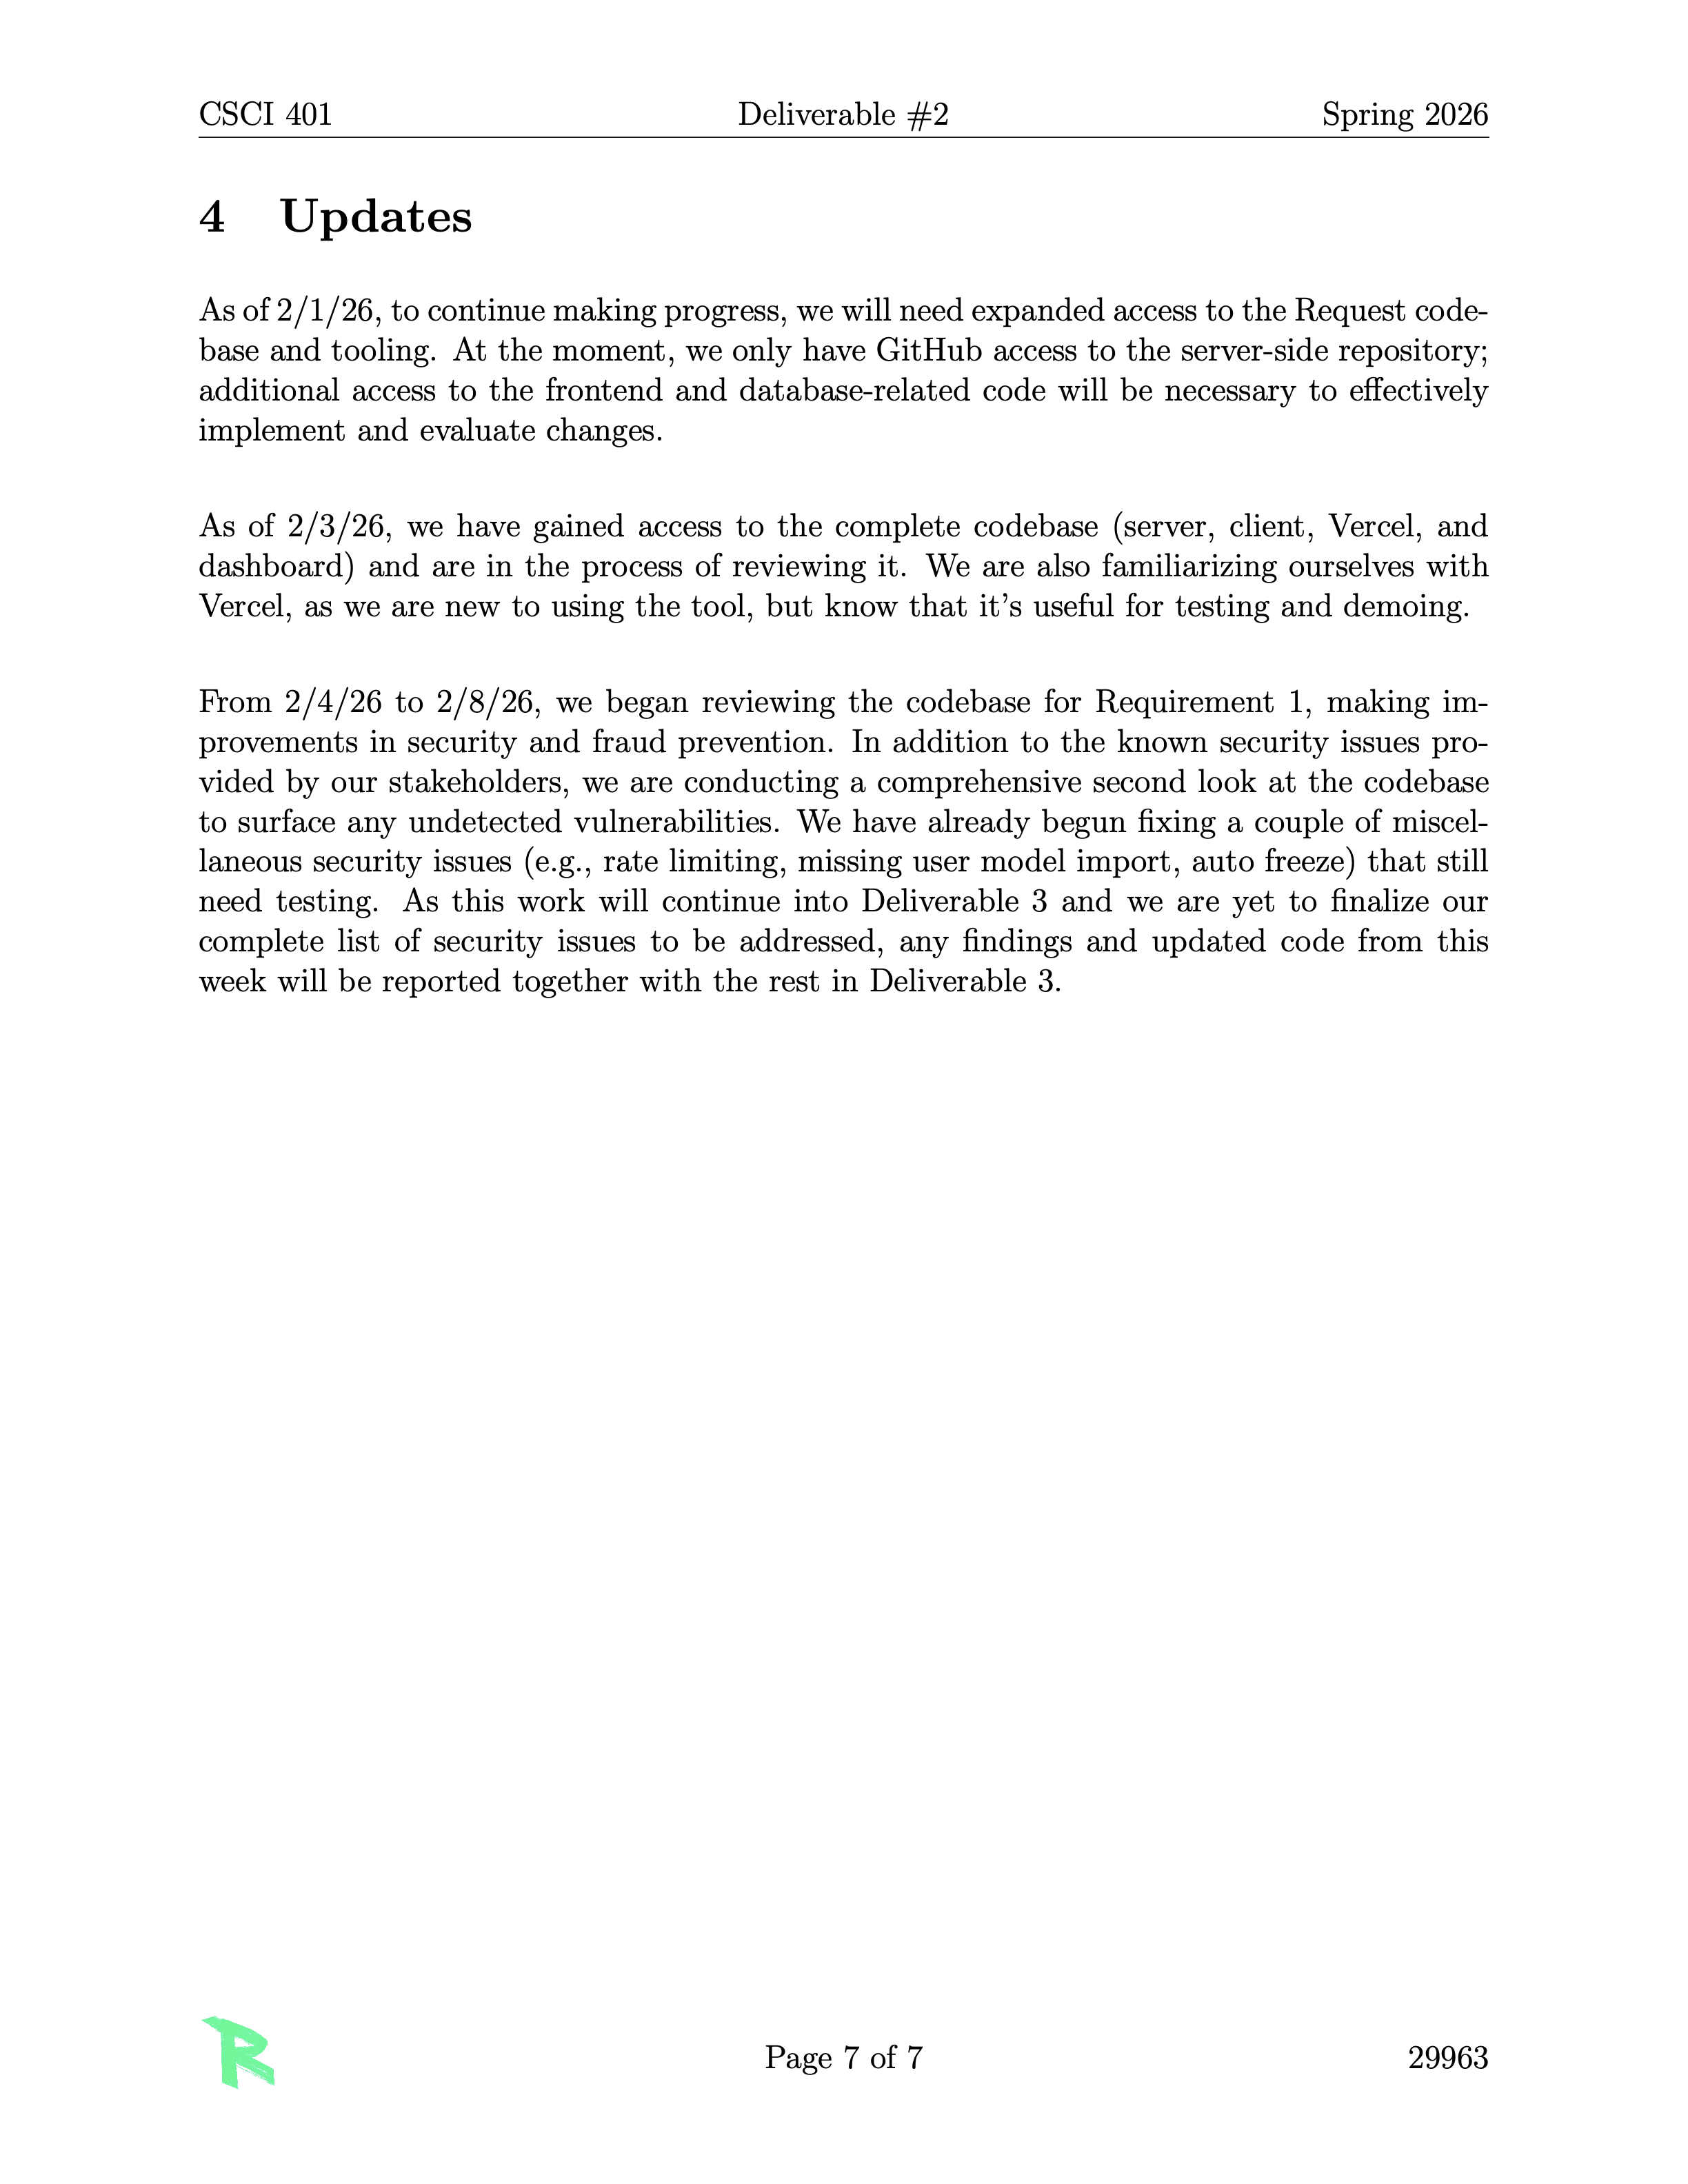
\includegraphics[width=0.48\textwidth,height=0.44\textheight,keepaspectratio]{images/deliverables/deliverable-2/Deliverable 2_7.png} &
            \end{tabular}\end{figure}\clearpage

            \subsubsection{Deliverable 3}

            \begin{figure}[H]\centering\setlength{\tabcolsep}{4pt}
            \begin{tabular}{cc}
            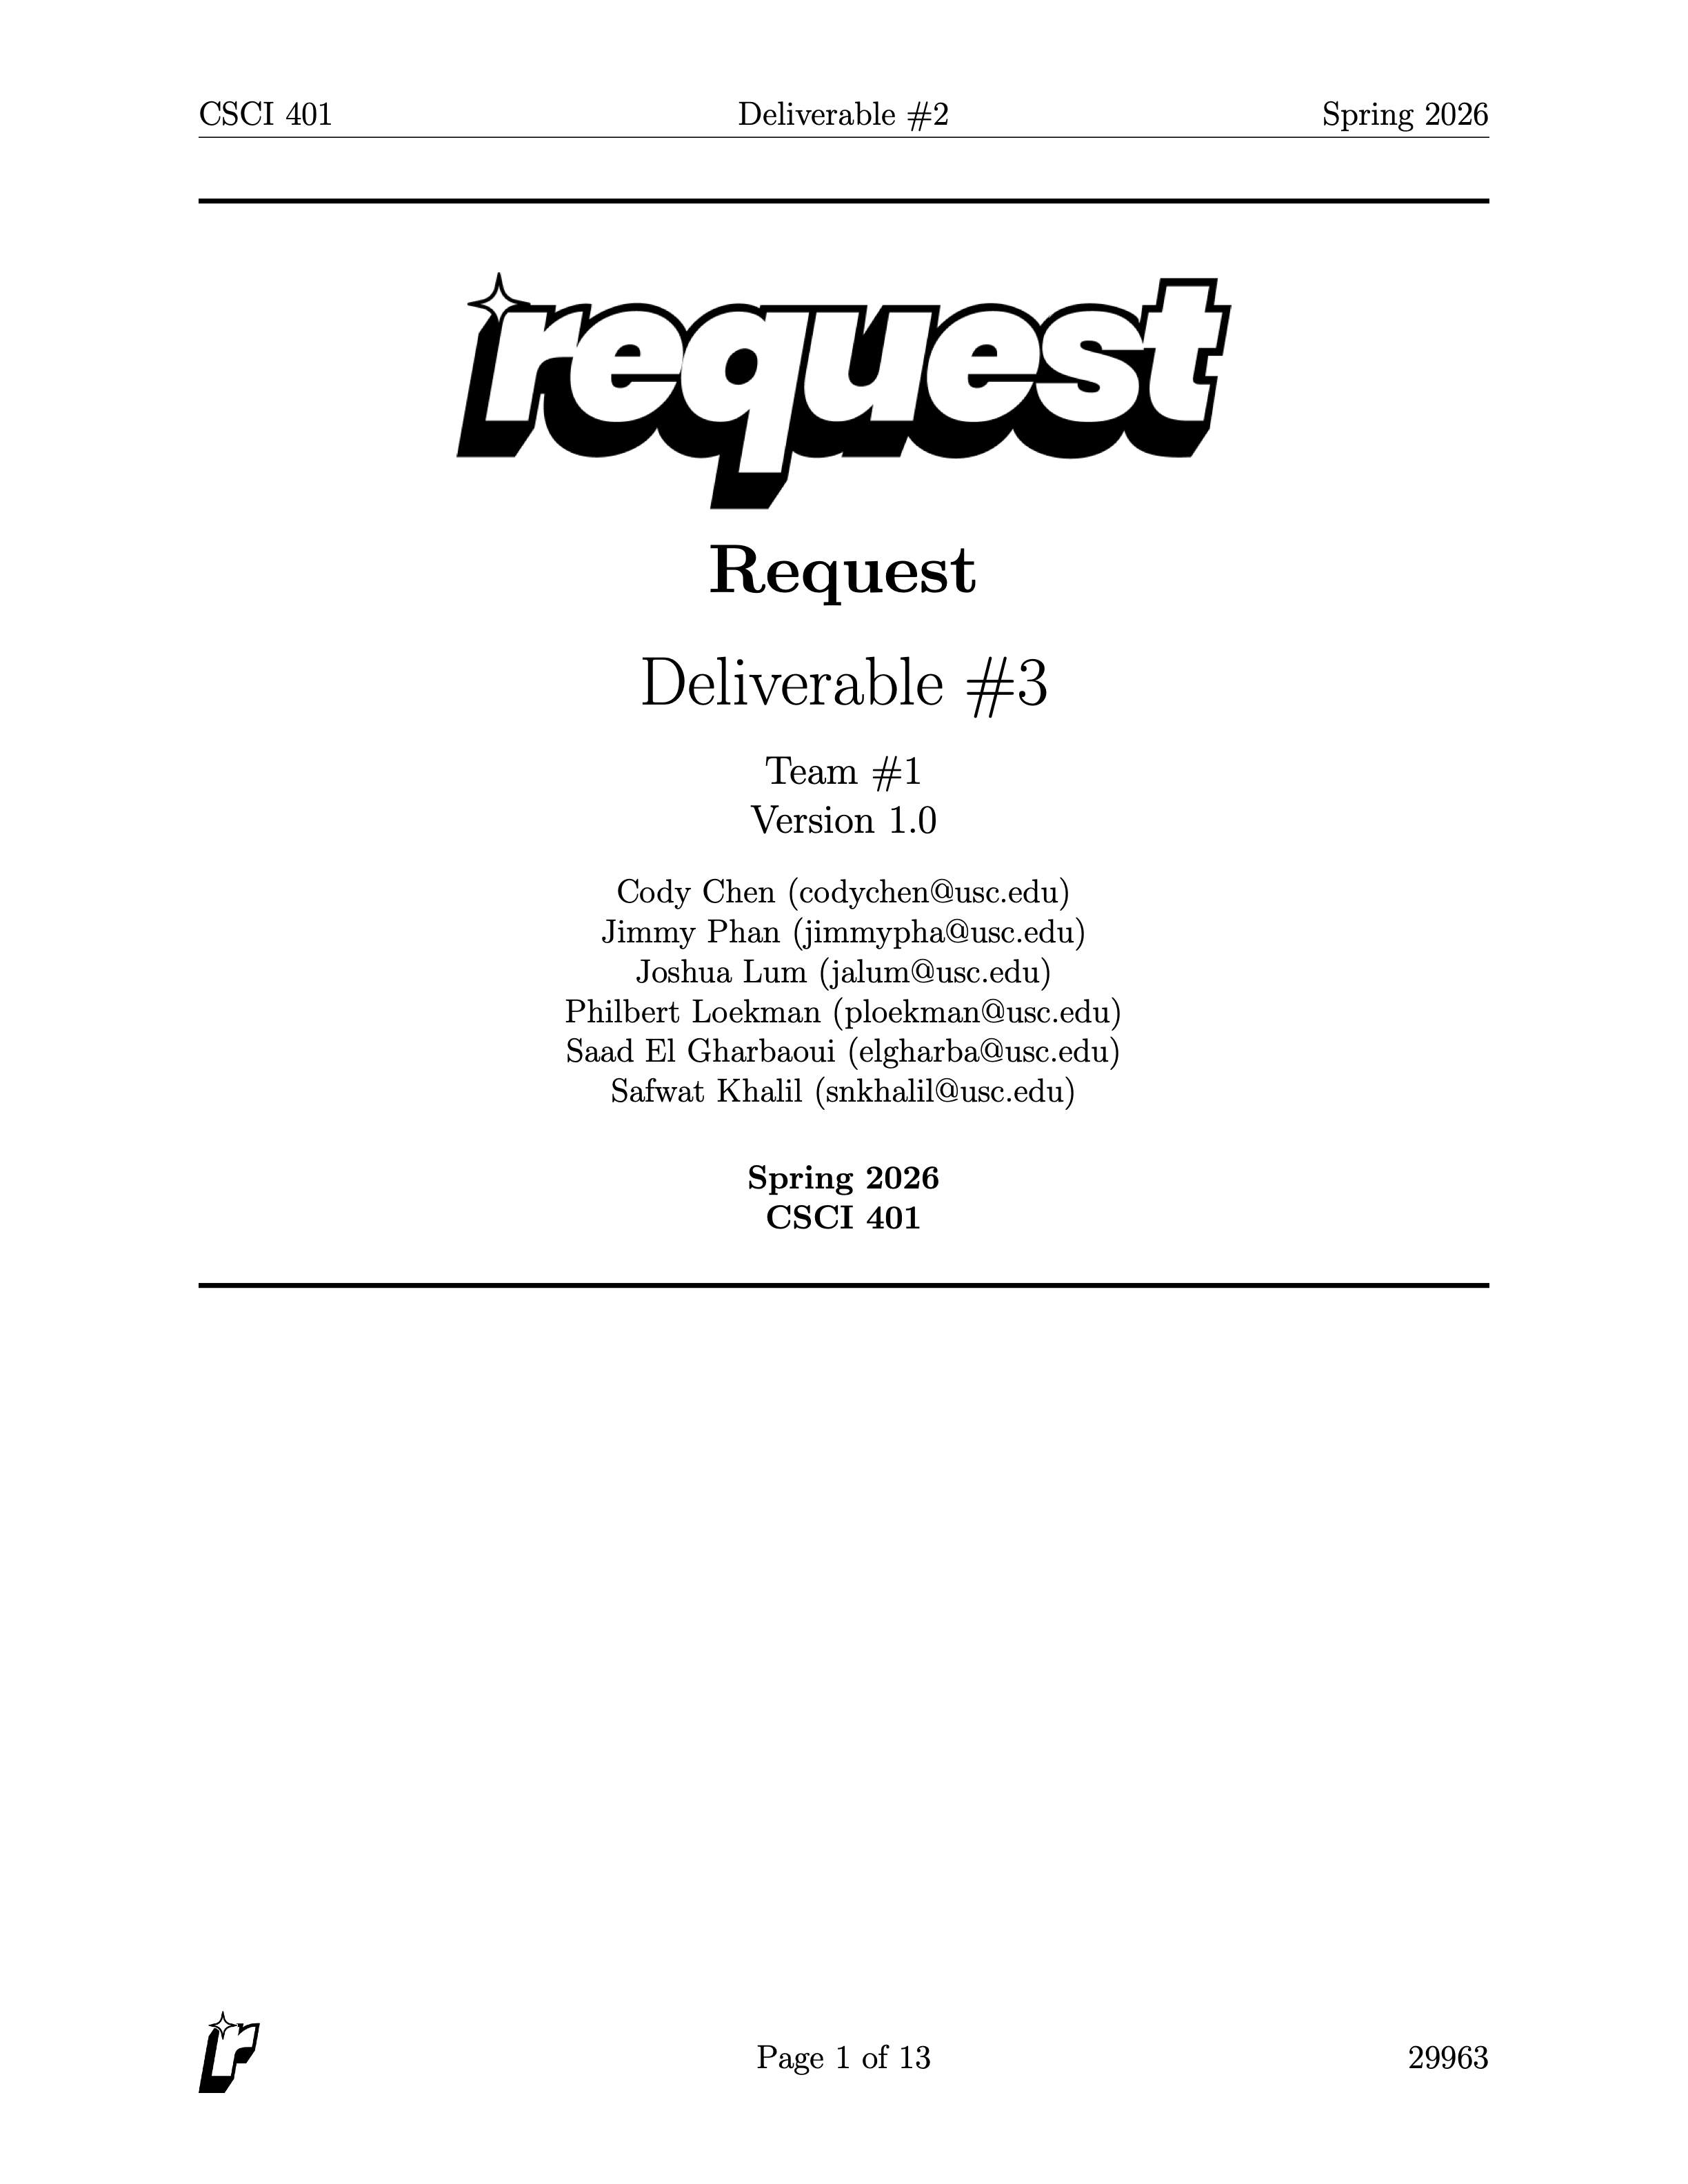
\includegraphics[width=0.48\textwidth,height=0.44\textheight,keepaspectratio]{images/deliverables/deliverable-3/Deliverable 3_1.png} &
            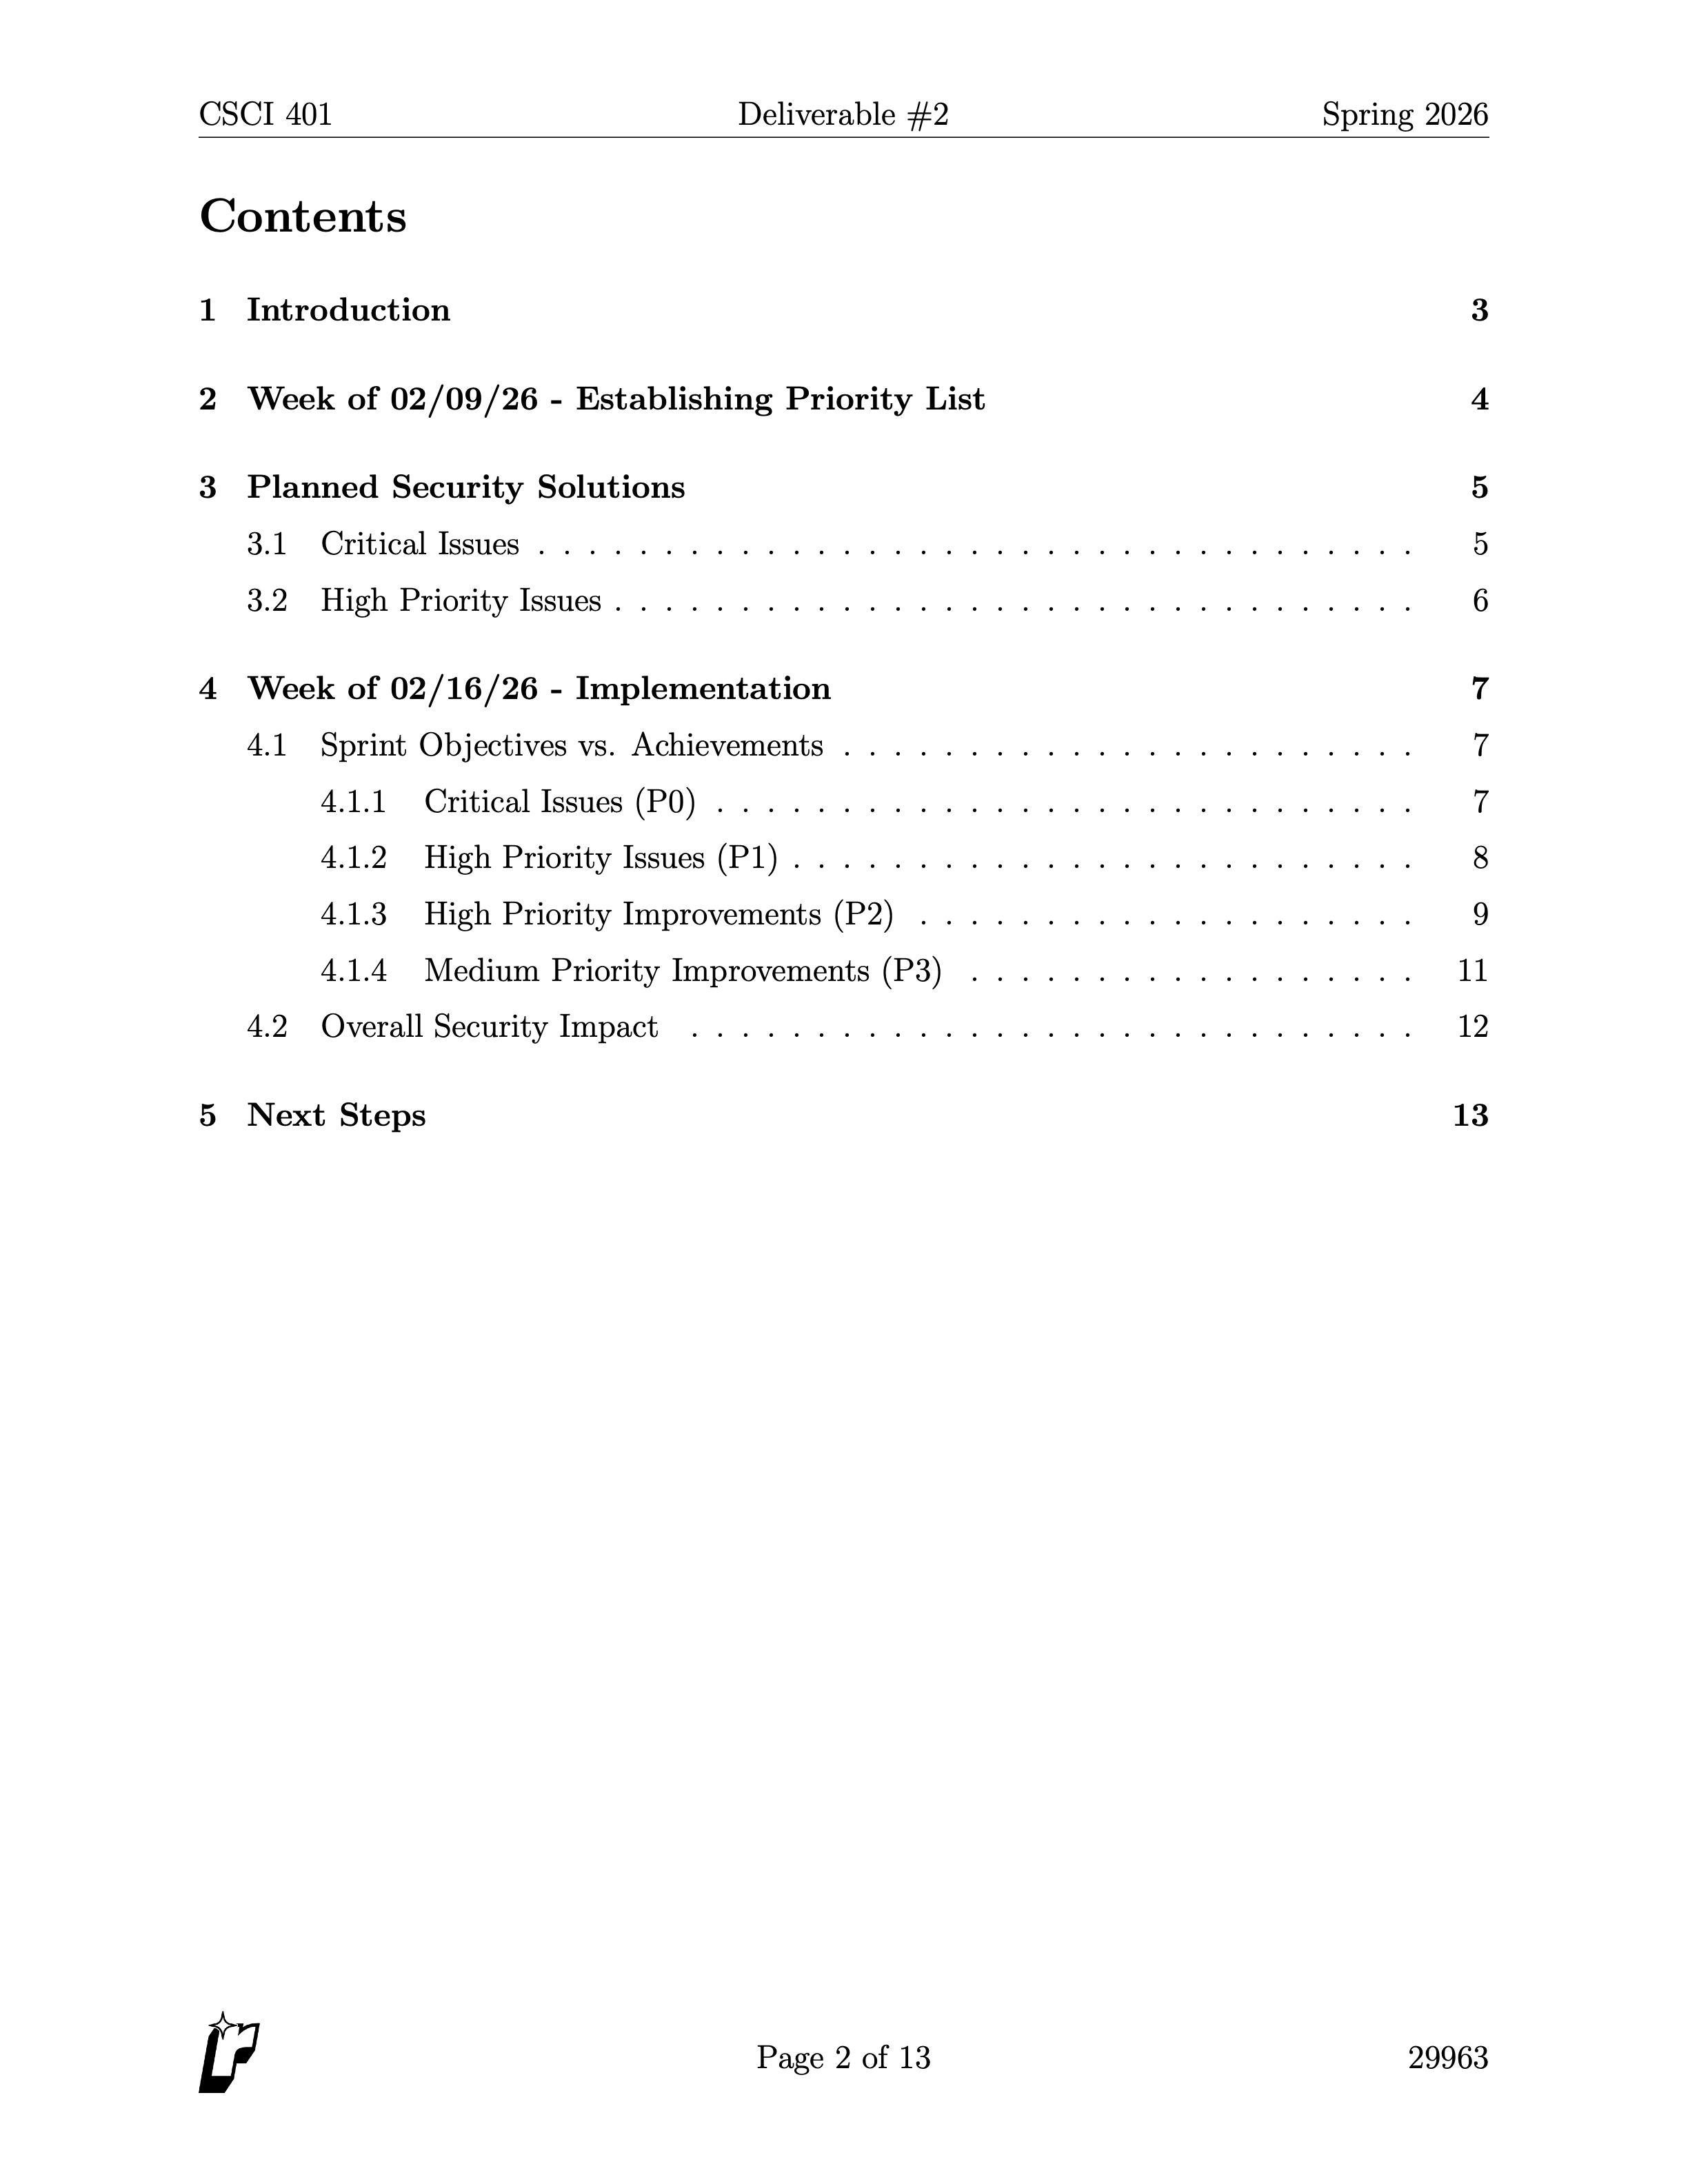
\includegraphics[width=0.48\textwidth,height=0.44\textheight,keepaspectratio]{images/deliverables/deliverable-3/Deliverable 3_2.png} \\[4pt]
            
\includegraphics[width=0.48\textwidth,height=0.44\textheight,keepaspectratio]{images/deliverables/deliverable-3/Deliverable 3_3.png} &
            
\includegraphics[width=0.48\textwidth,height=0.44\textheight,keepaspectratio]{images/deliverables/deliverable-3/Deliverable 3_4.png}
            \end{tabular}\end{figure}\clearpage

            \begin{figure}[H]\centering\setlength{\tabcolsep}{4pt}
            \begin{tabular}{cc}
            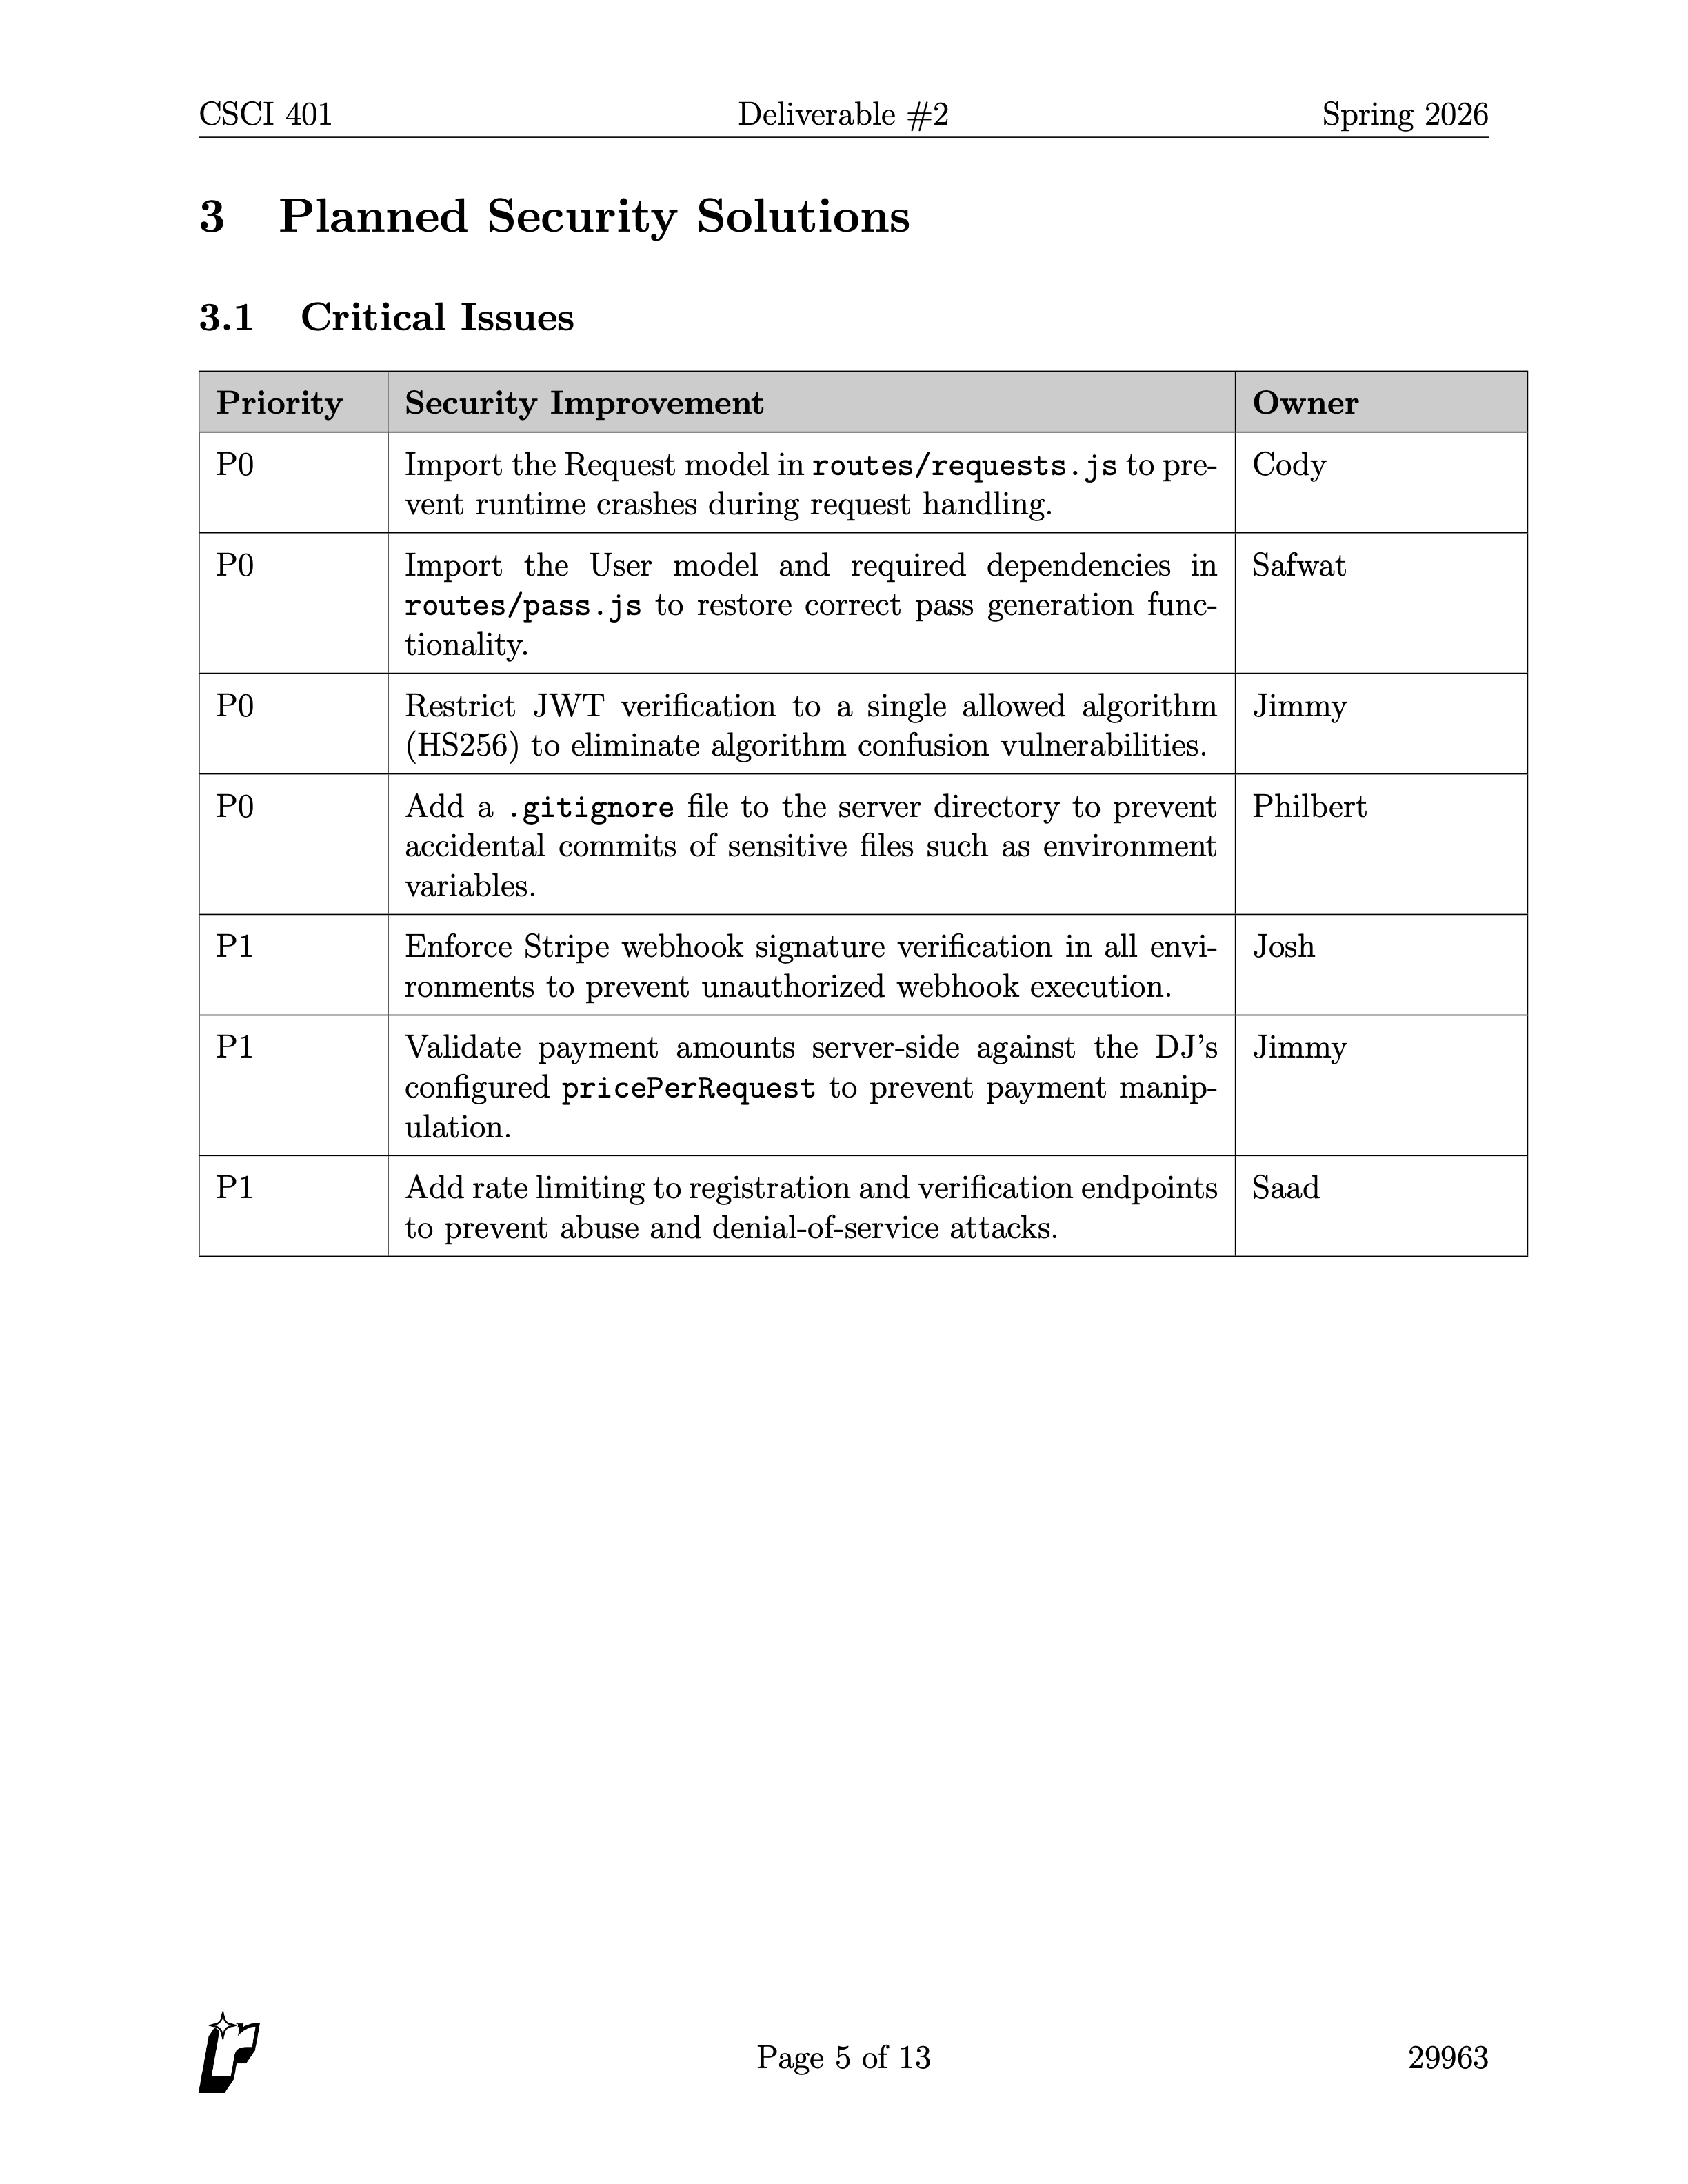
\includegraphics[width=0.48\textwidth,height=0.44\textheight,keepaspectratio]{images/deliverables/deliverable-3/Deliverable 3_5.png} &
            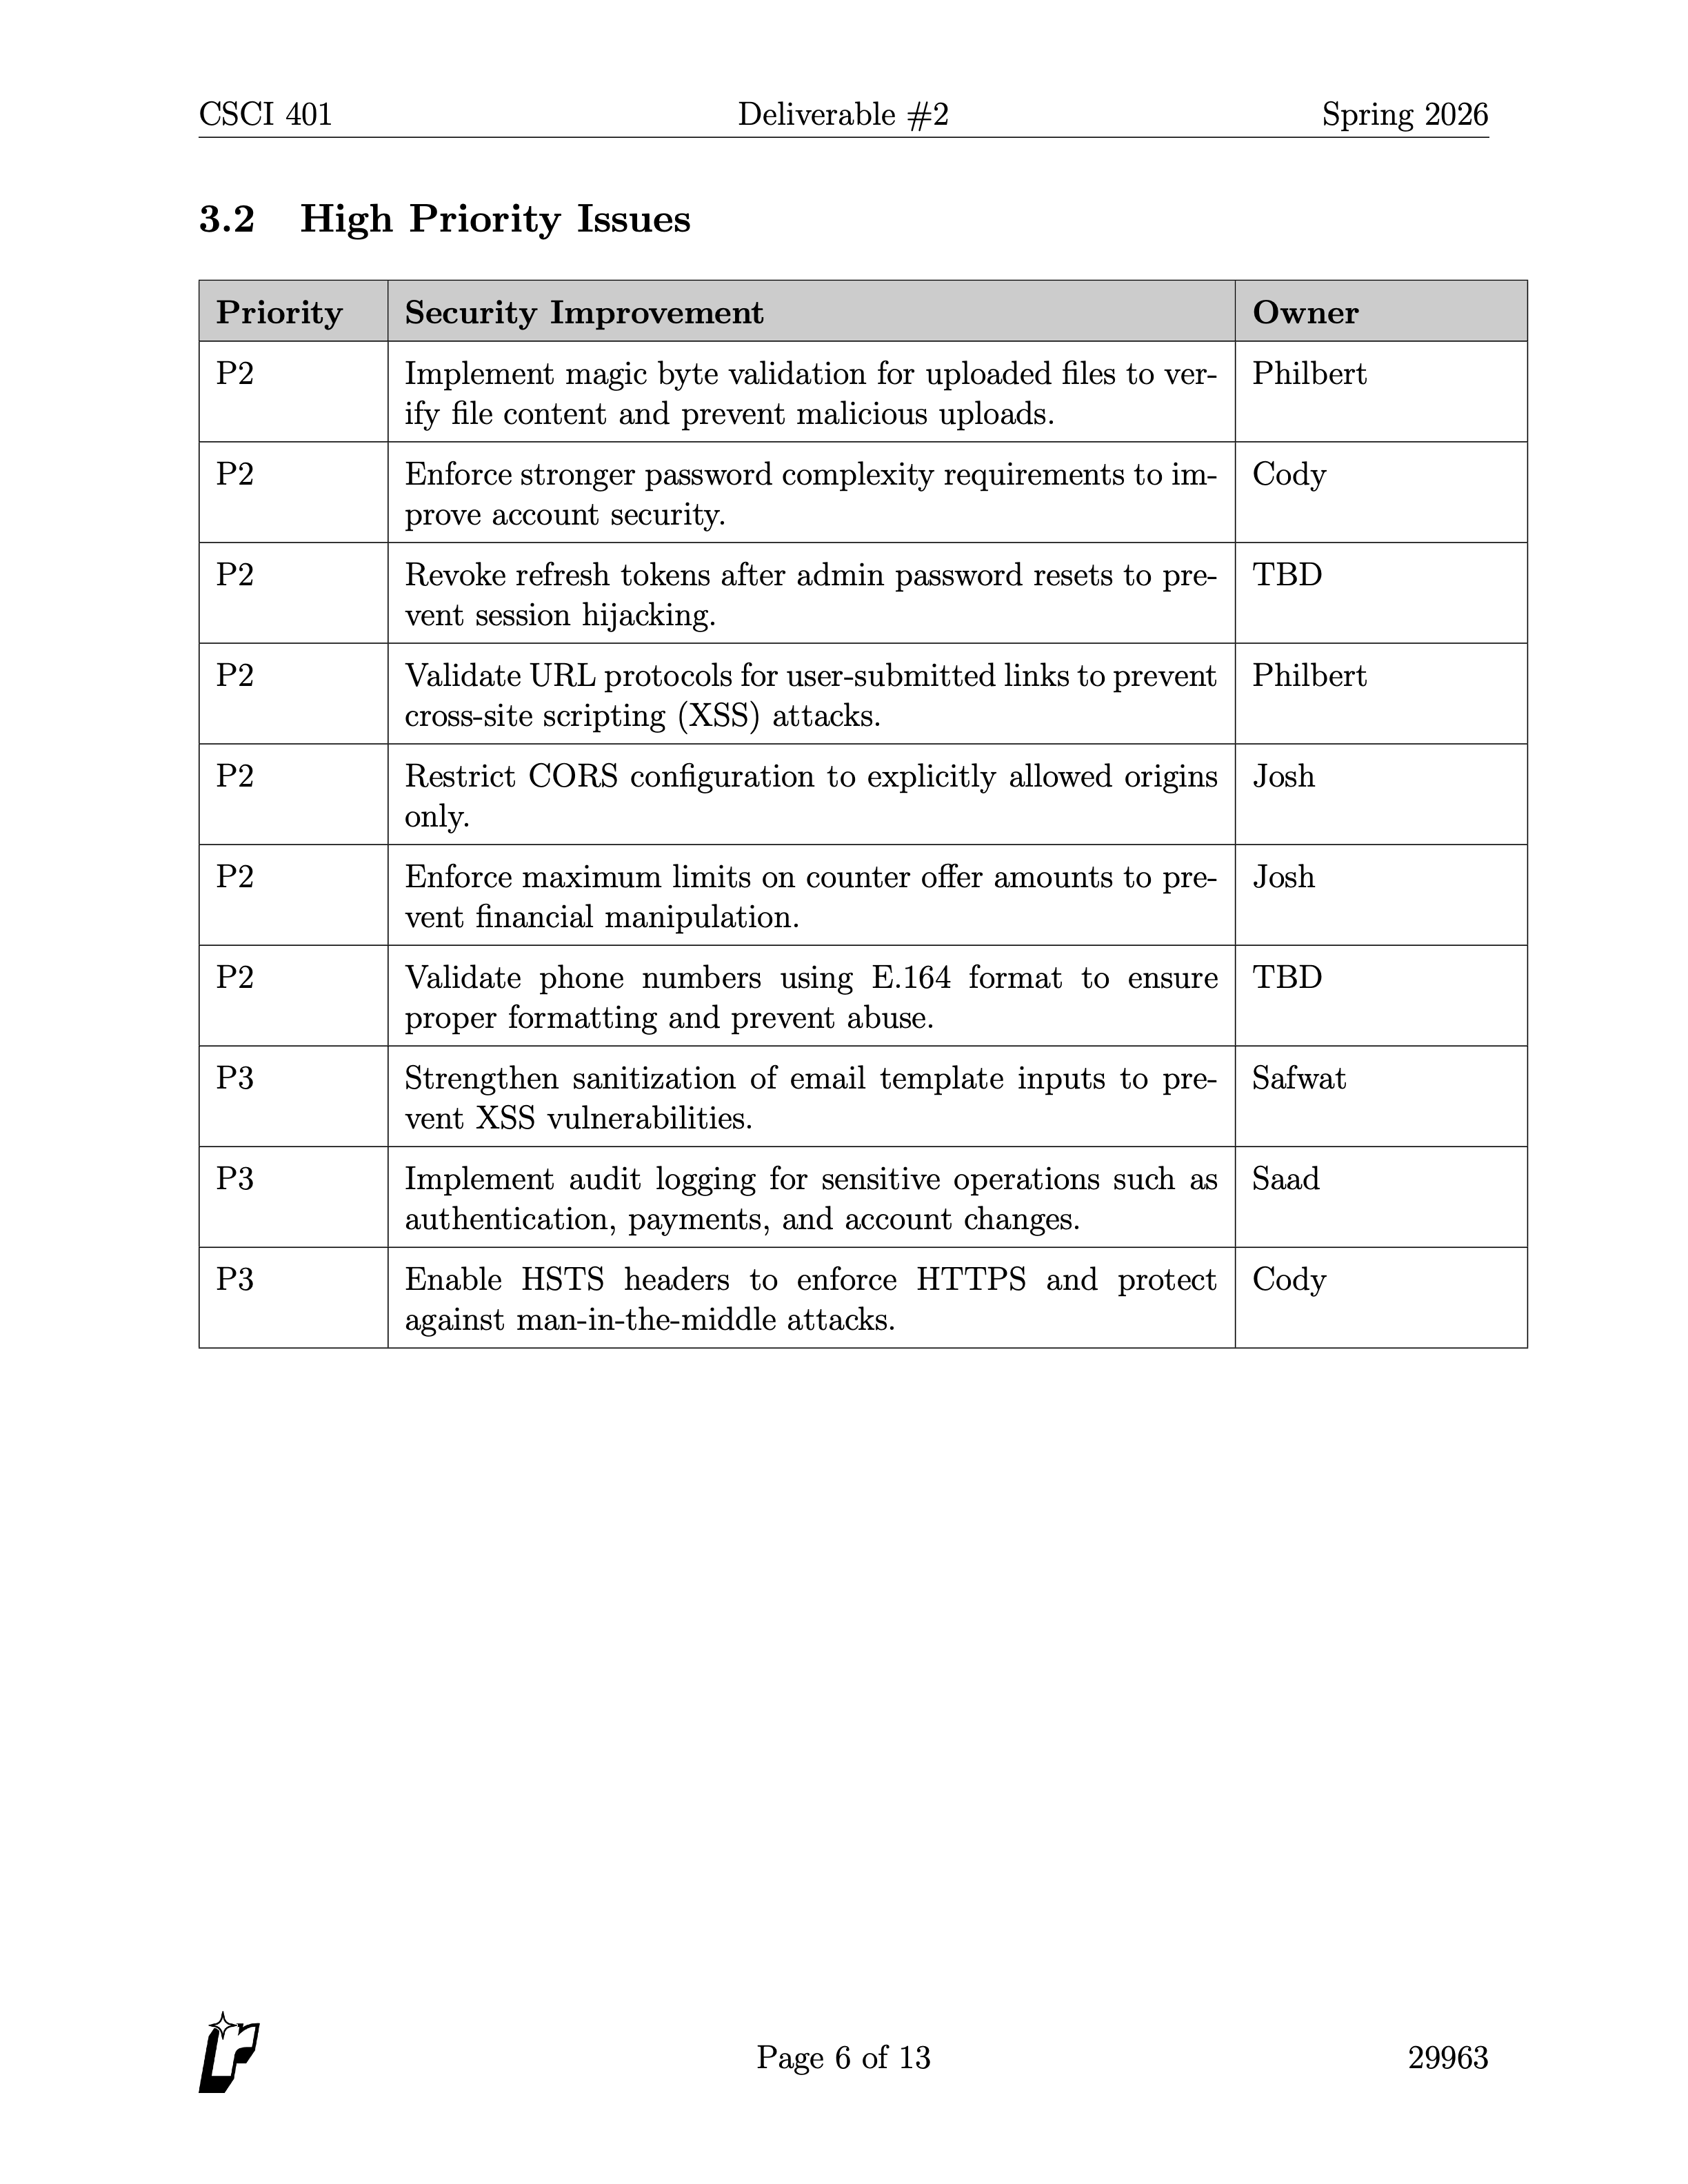
\includegraphics[width=0.48\textwidth,height=0.44\textheight,keepaspectratio]{images/deliverables/deliverable-3/Deliverable 3_6.png} \\[4pt]
            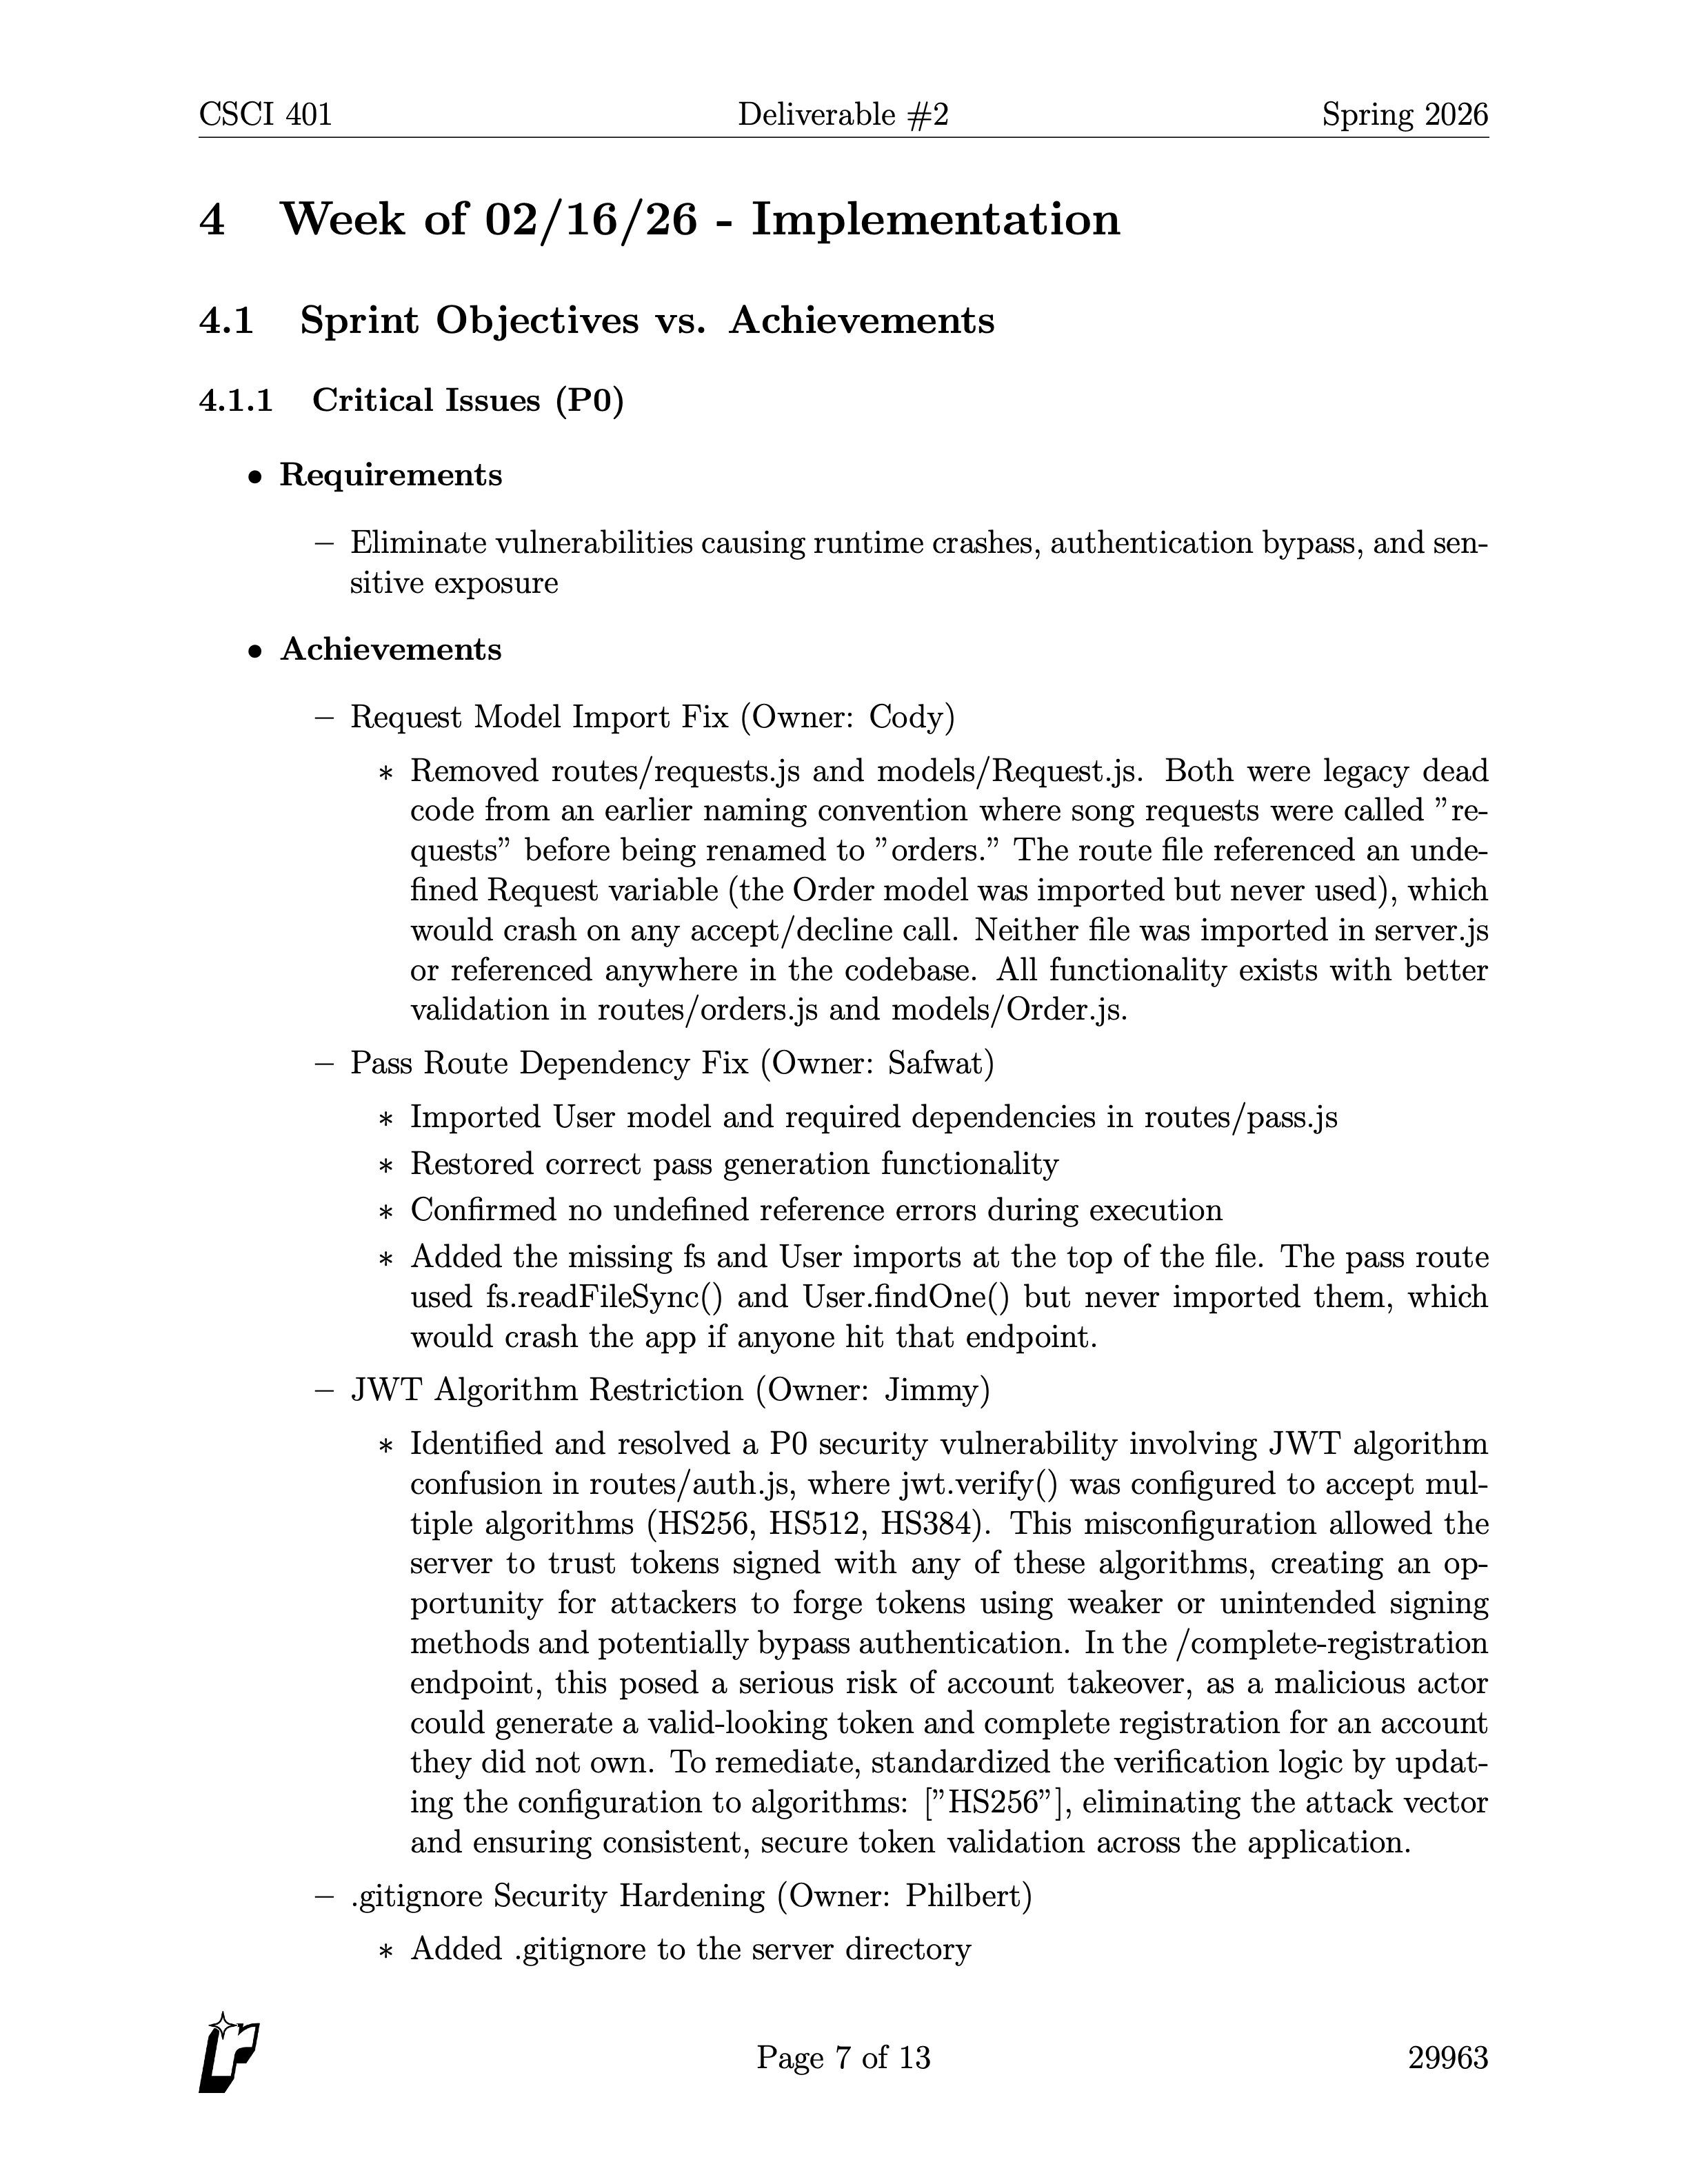
\includegraphics[width=0.48\textwidth,height=0.44\textheight,keepaspectratio]{images/deliverables/deliverable-3/Deliverable 3_7.png} &
            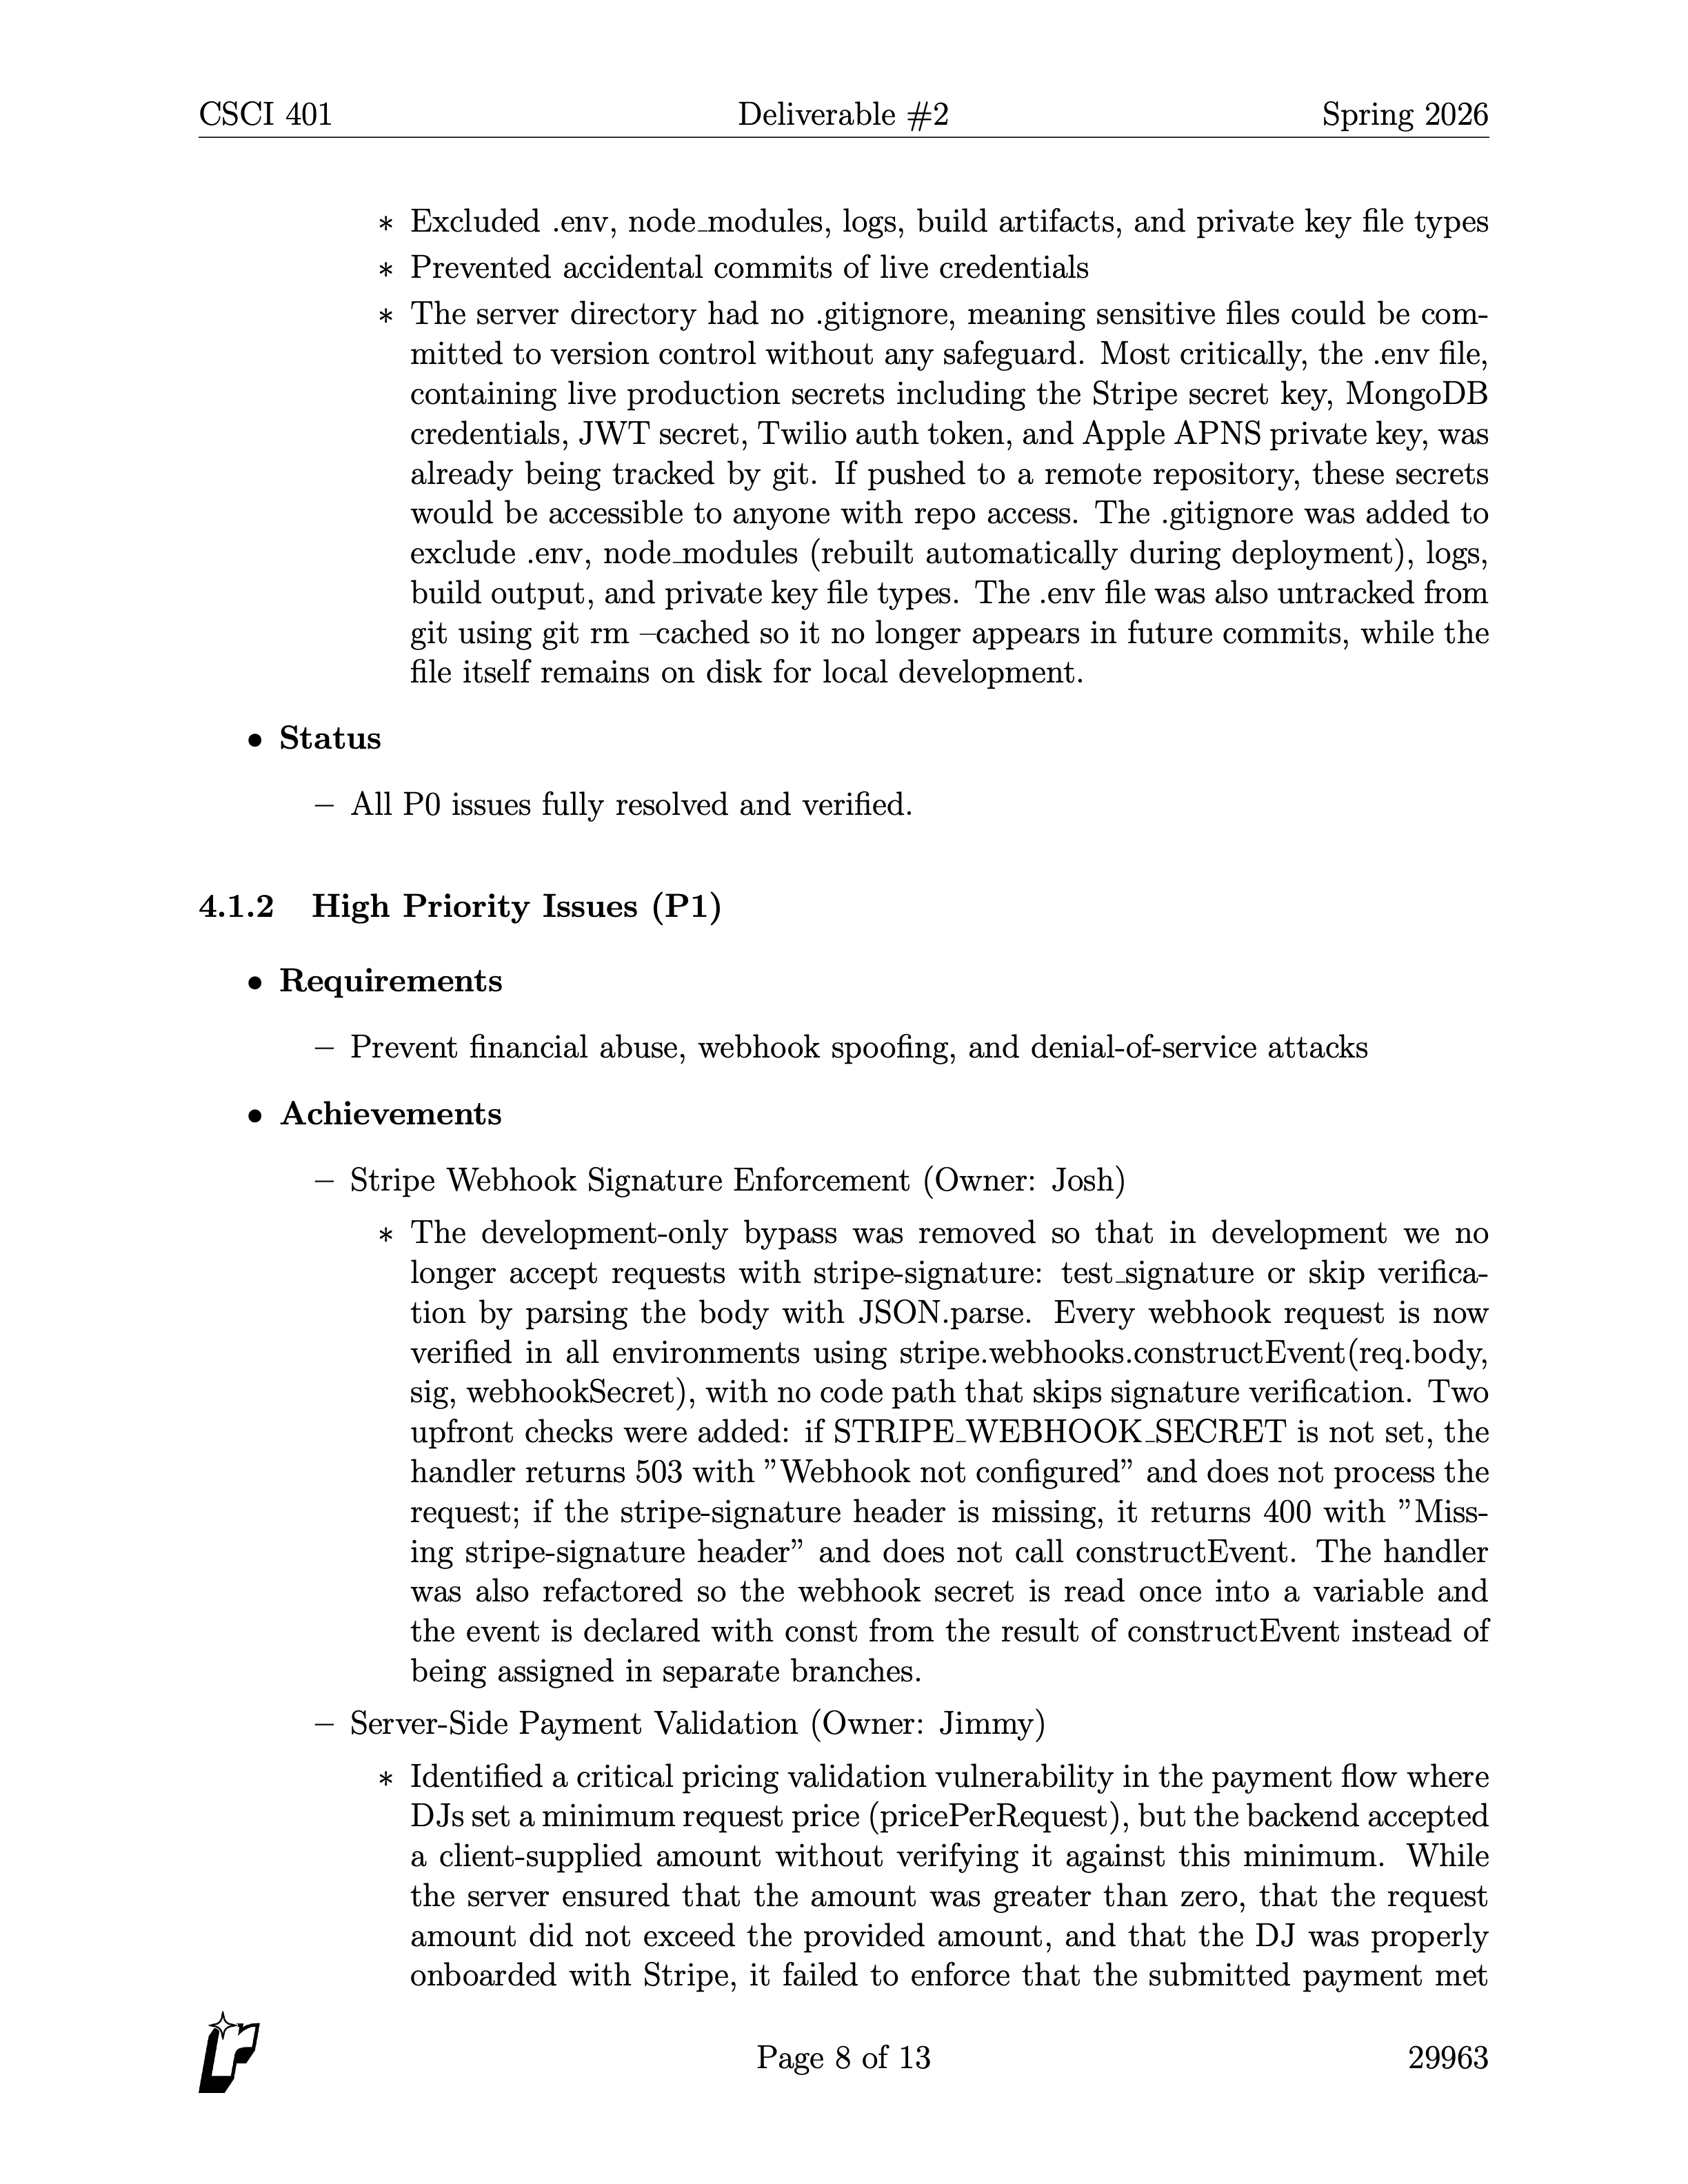
\includegraphics[width=0.48\textwidth,height=0.44\textheight,keepaspectratio]{images/deliverables/deliverable-3/Deliverable 3_8.png}
            \end{tabular}\end{figure}\clearpage

            \begin{figure}[H]\centering\setlength{\tabcolsep}{4pt}
            \begin{tabular}{cc}
            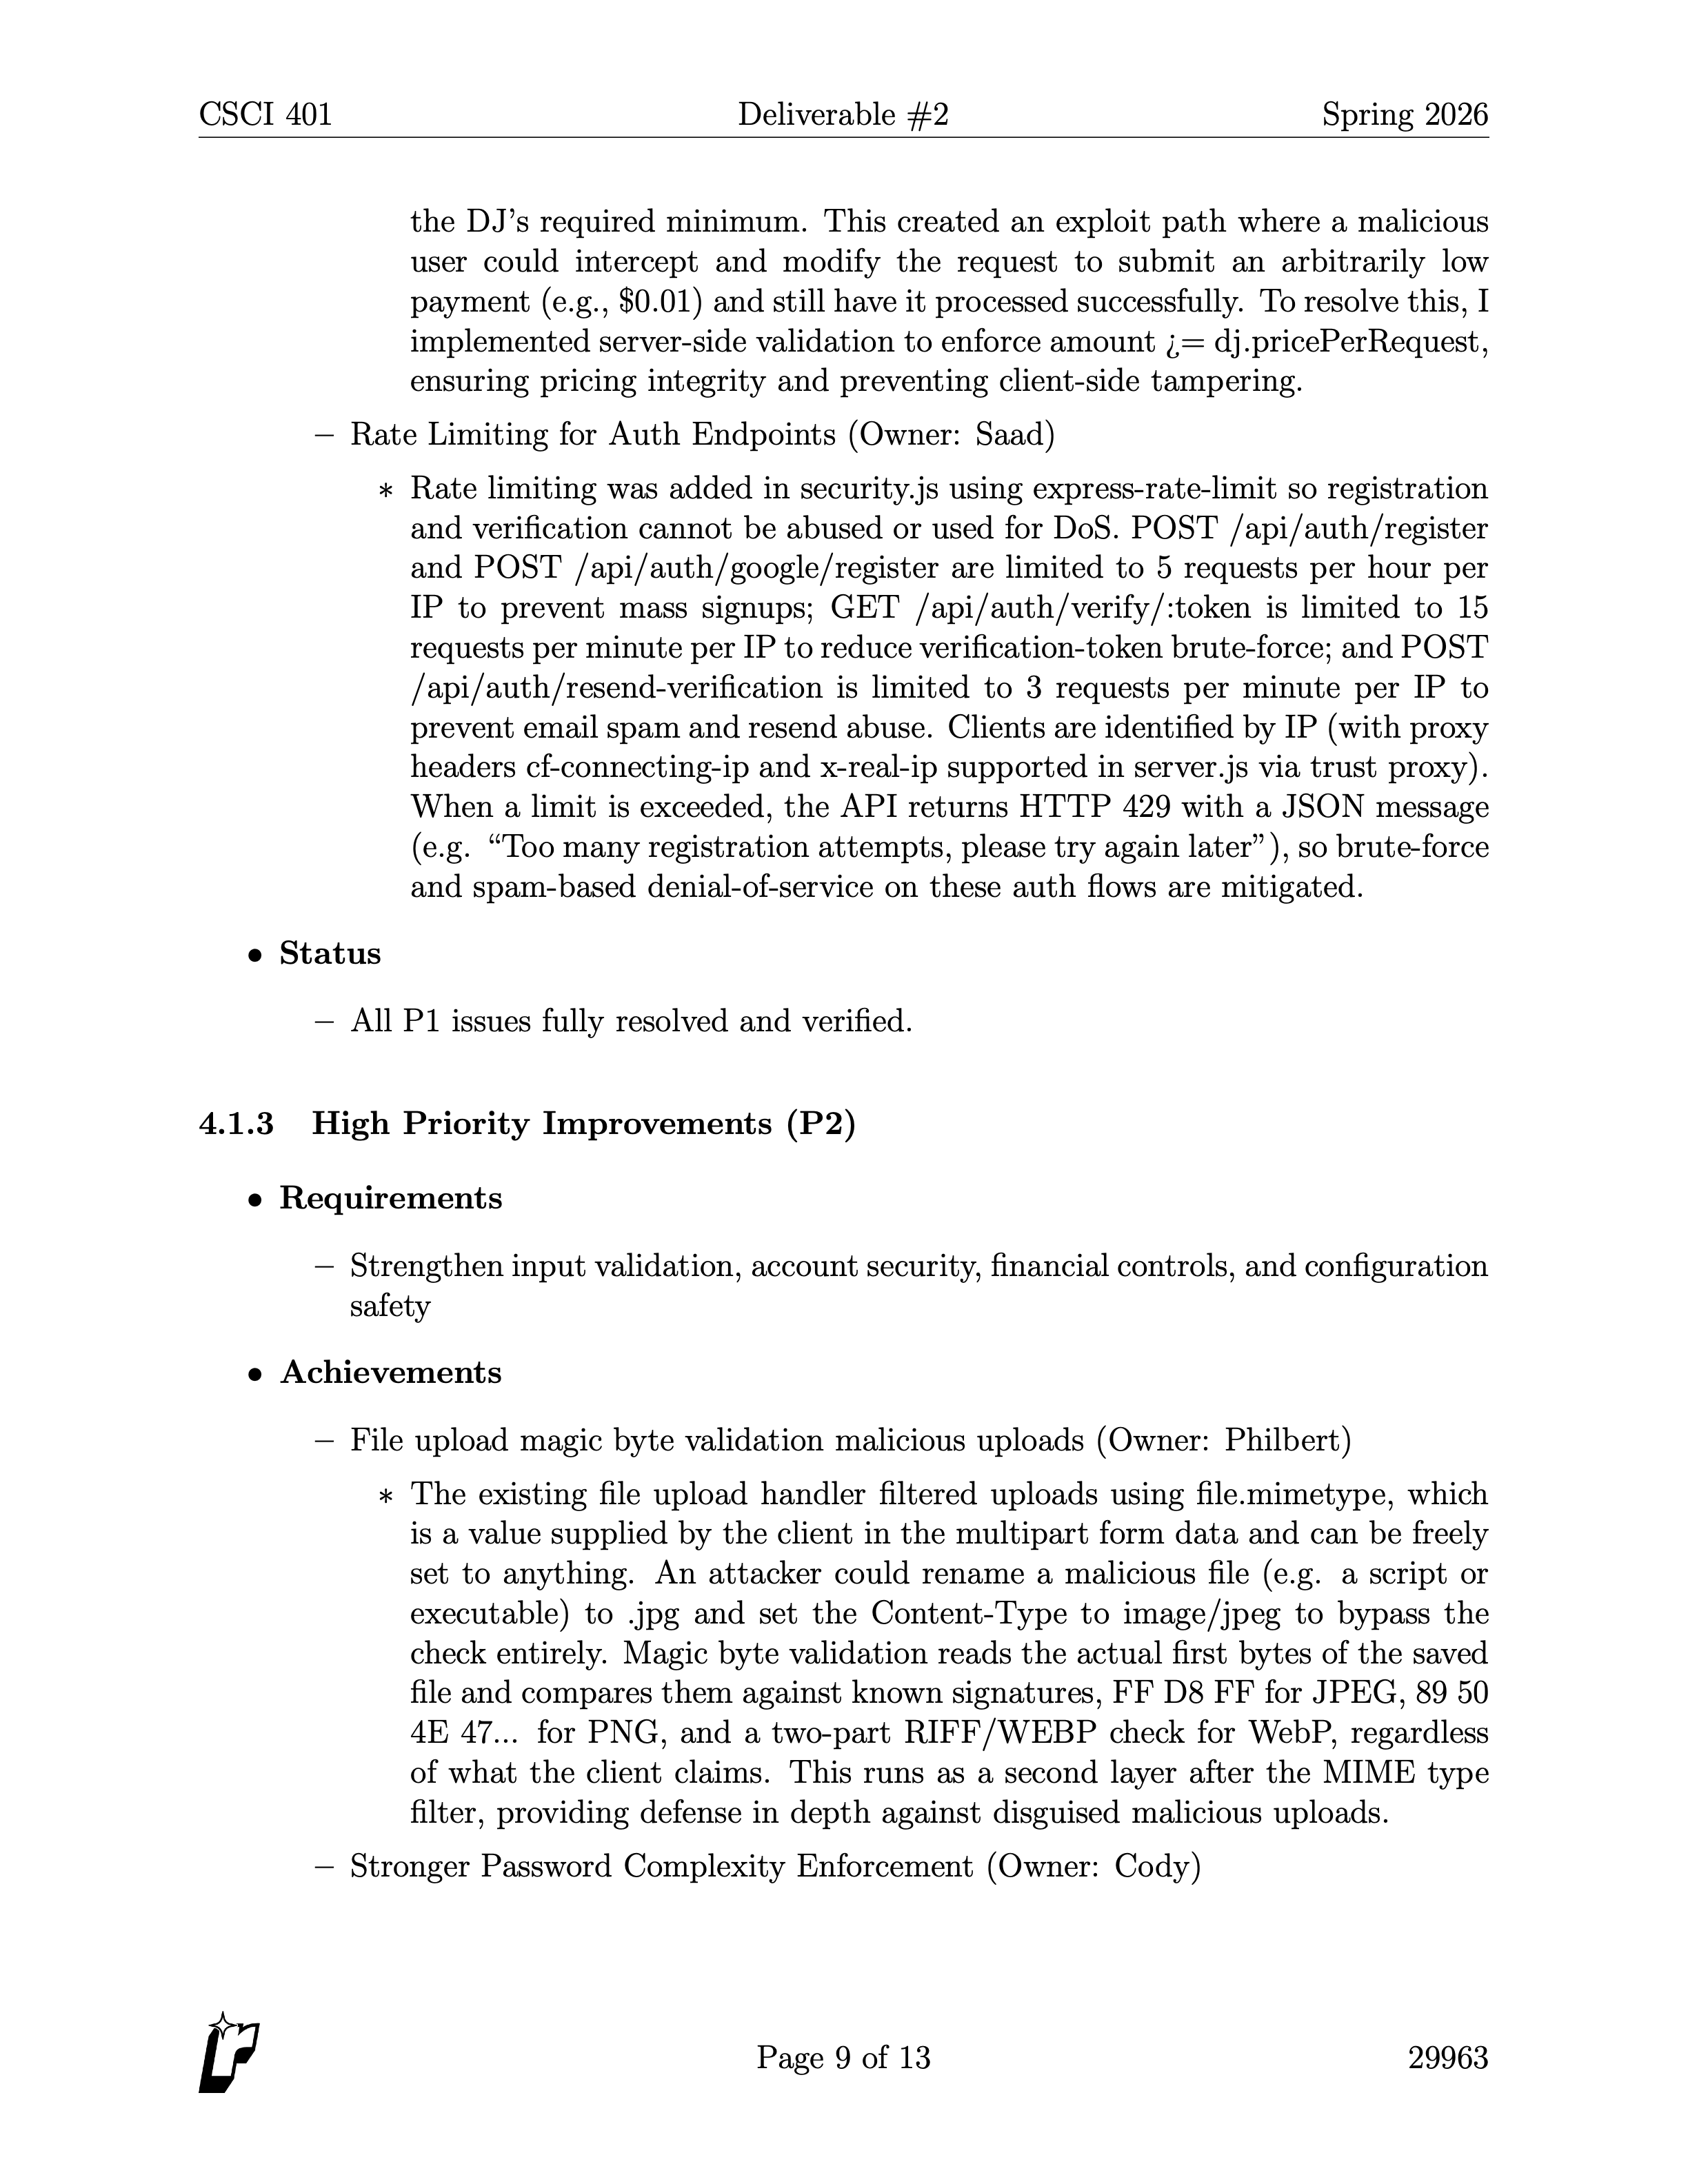
\includegraphics[width=0.48\textwidth,height=0.44\textheight,keepaspectratio]{images/deliverables/deliverable-3/Deliverable 3_9.png} &
            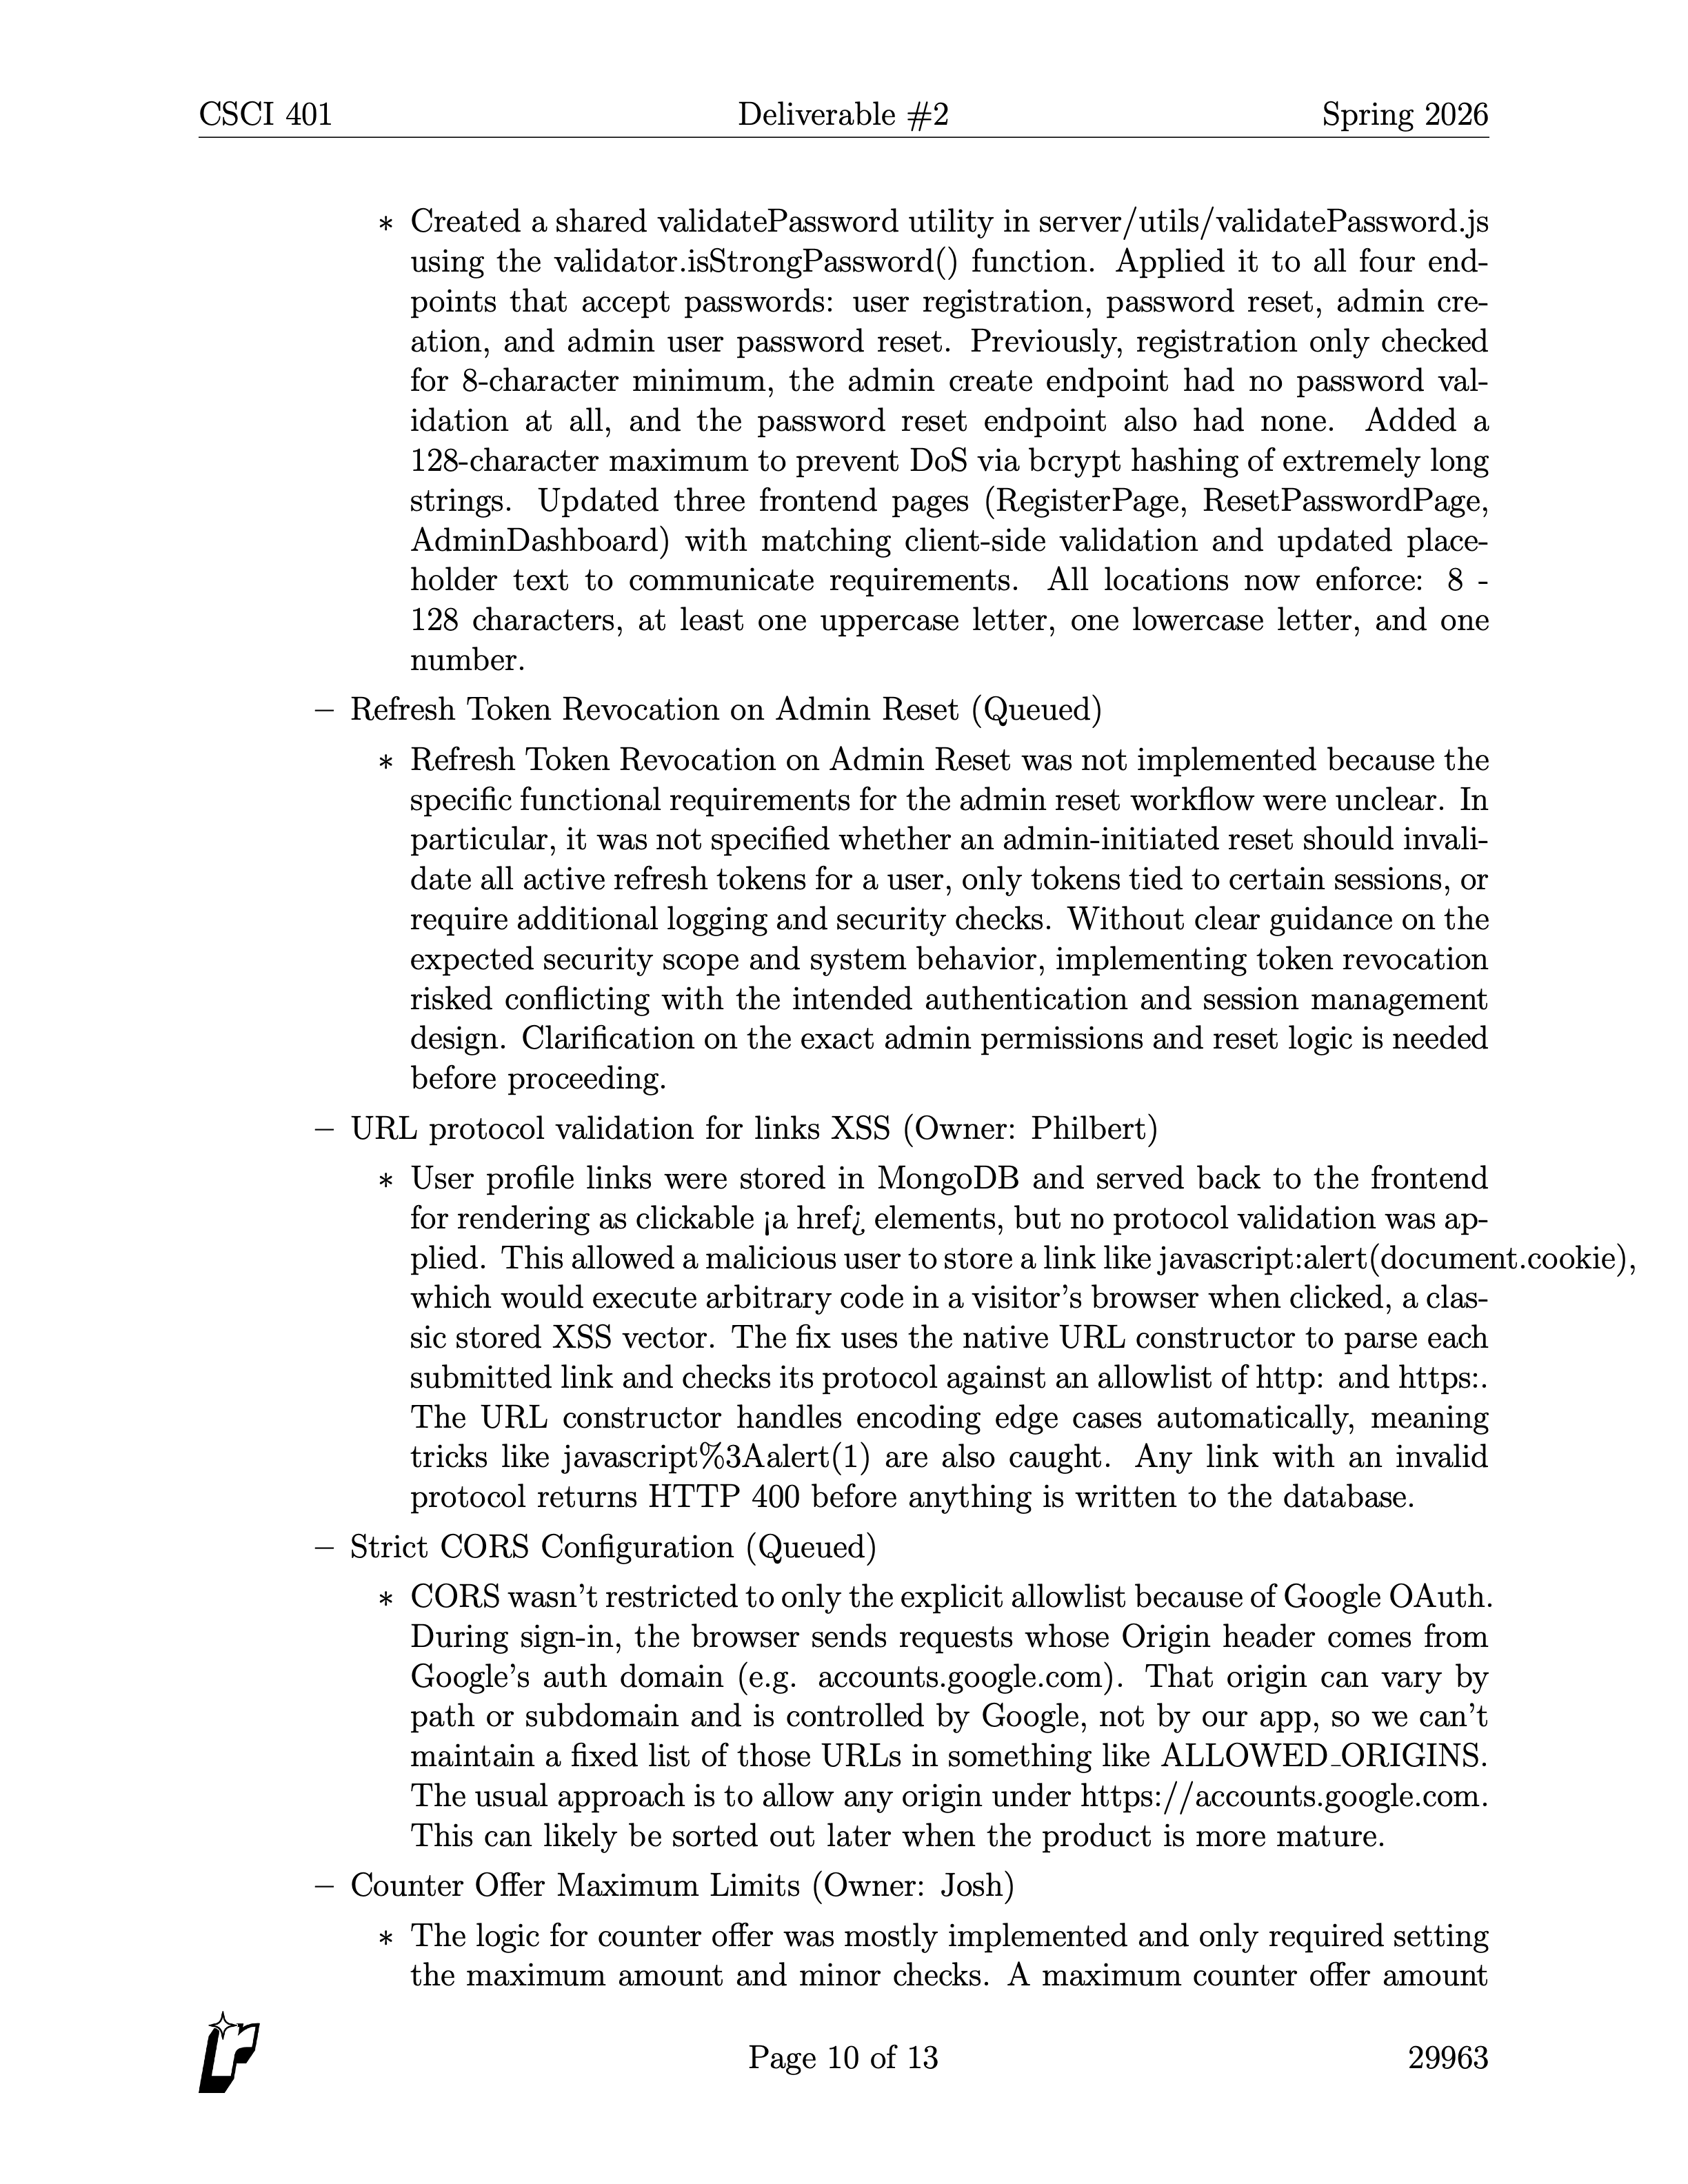
\includegraphics[width=0.48\textwidth,height=0.44\textheight,keepaspectratio]{images/deliverables/deliverable-3/Deliverable 3_10.png} \\[4pt]
            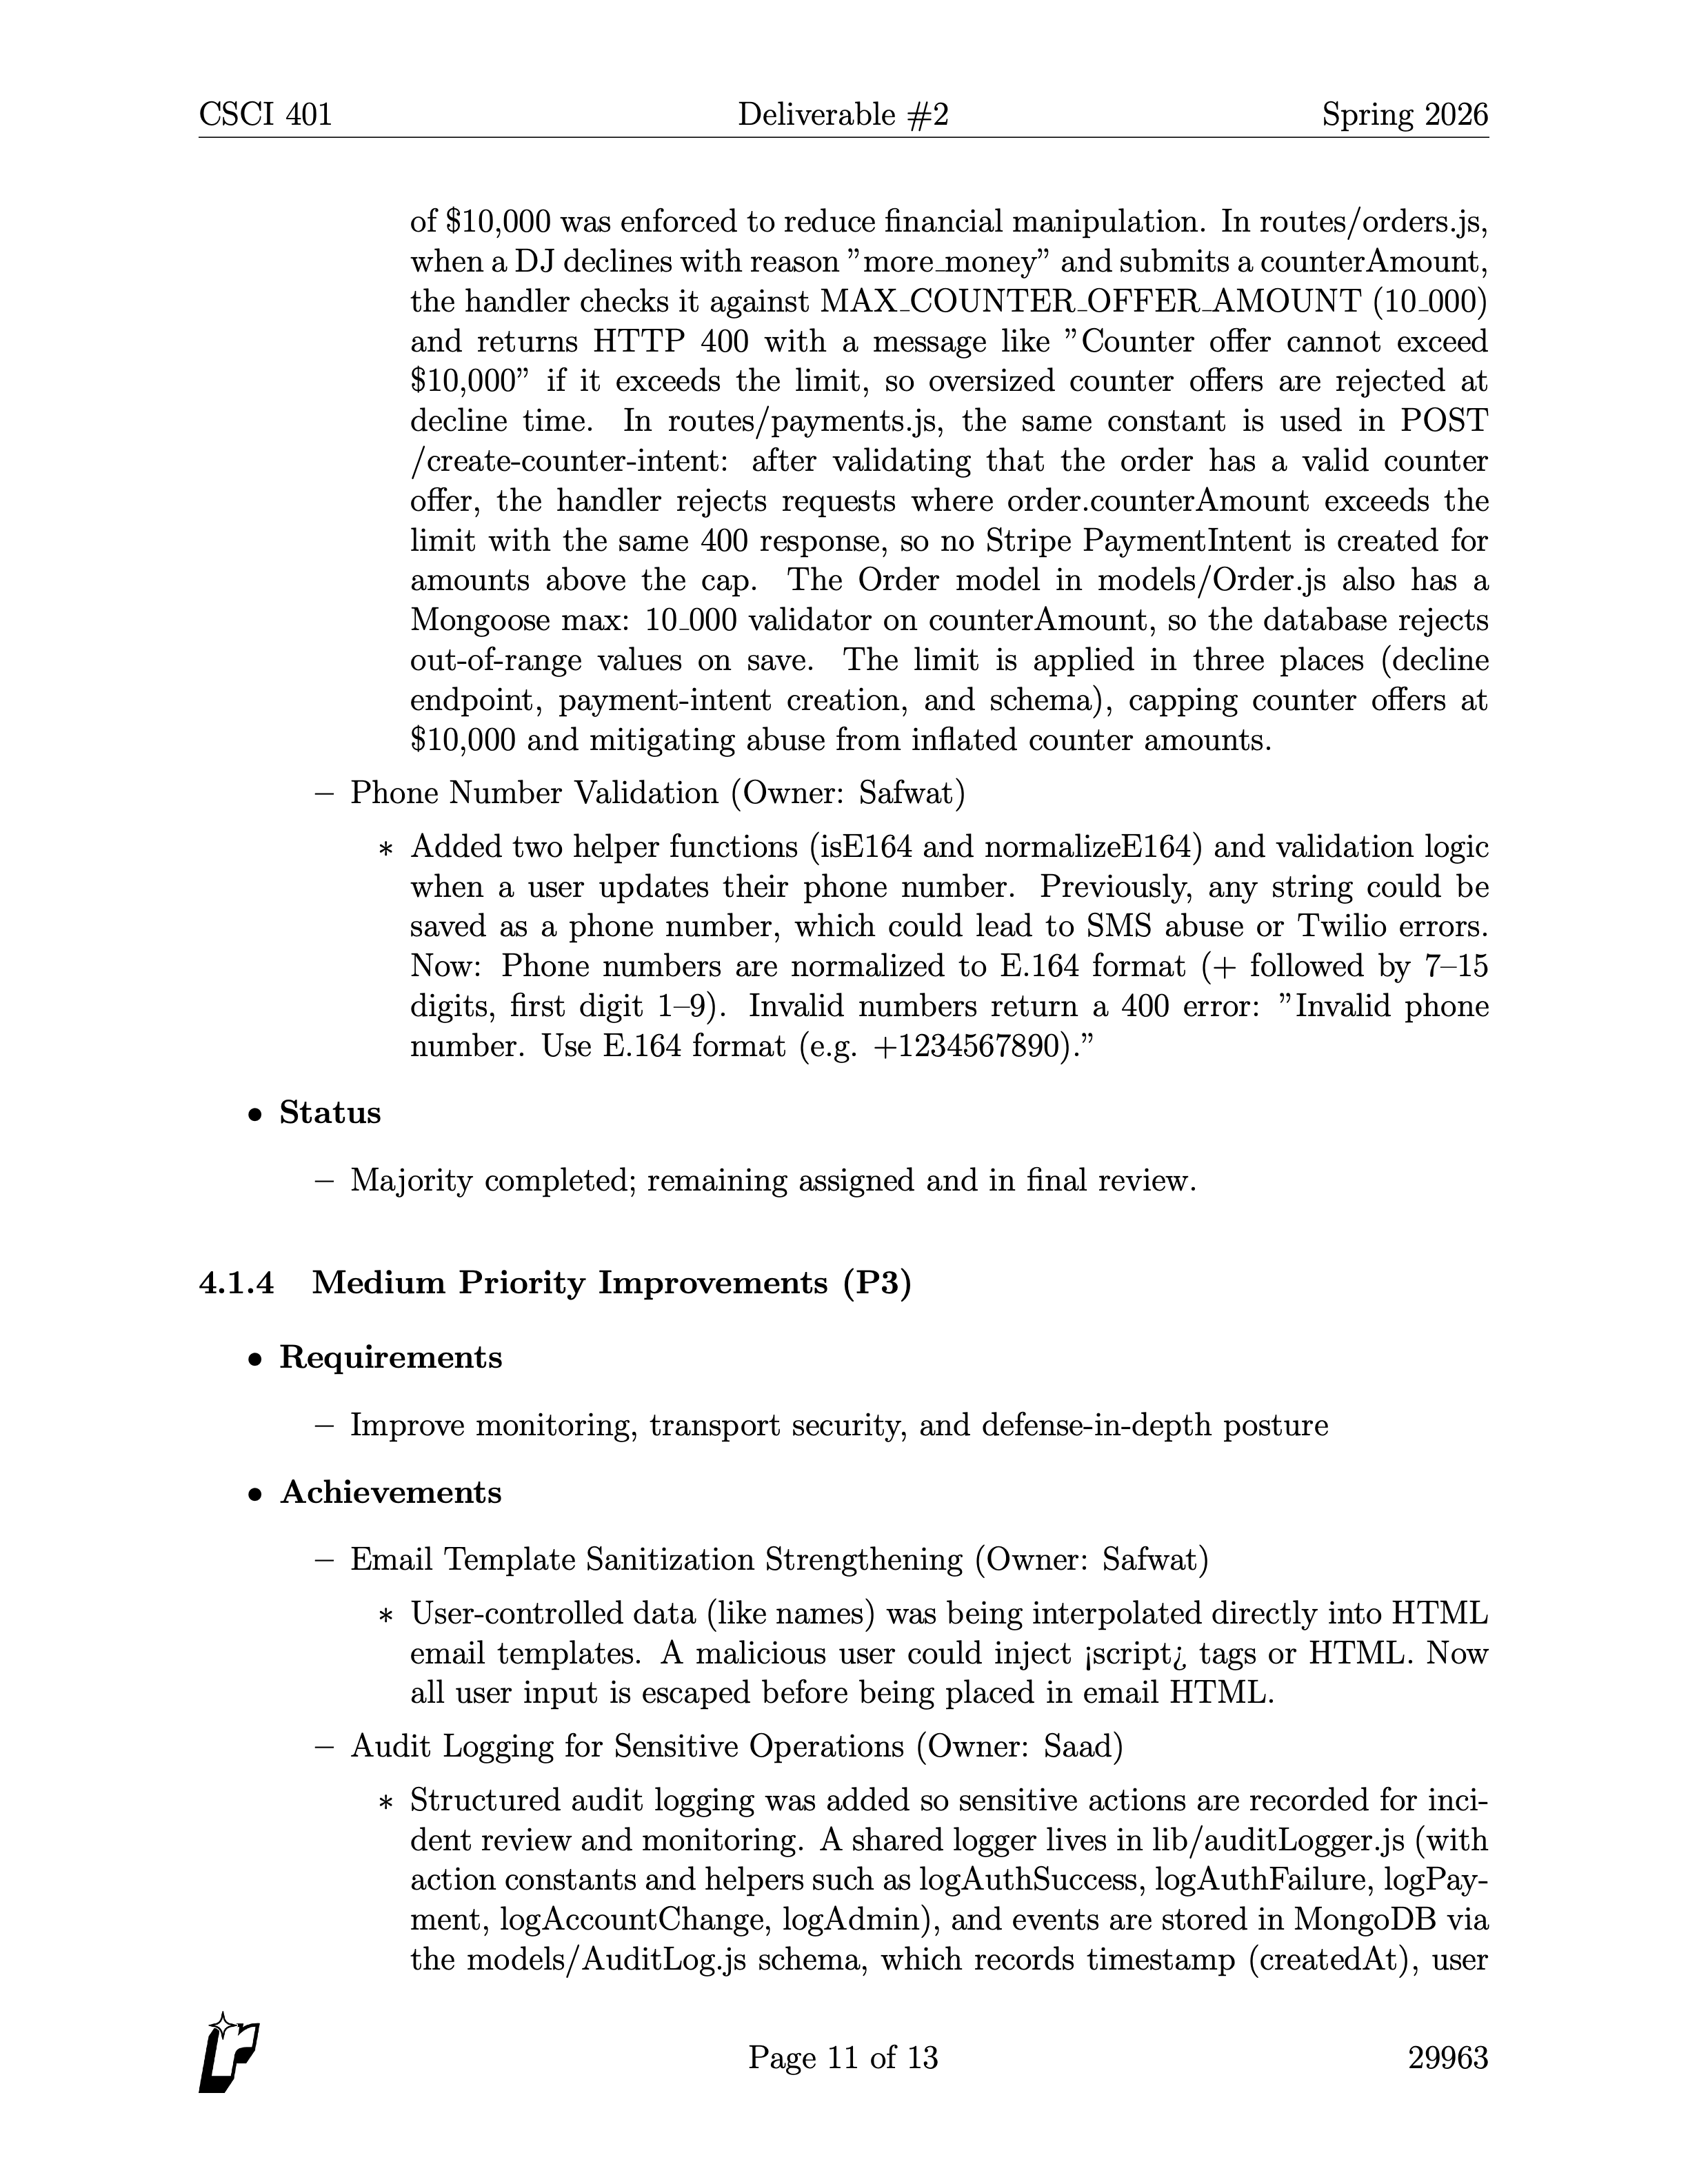
\includegraphics[width=0.48\textwidth,height=0.44\textheight,keepaspectratio]{images/deliverables/deliverable-3/Deliverable 3_11.png} &
            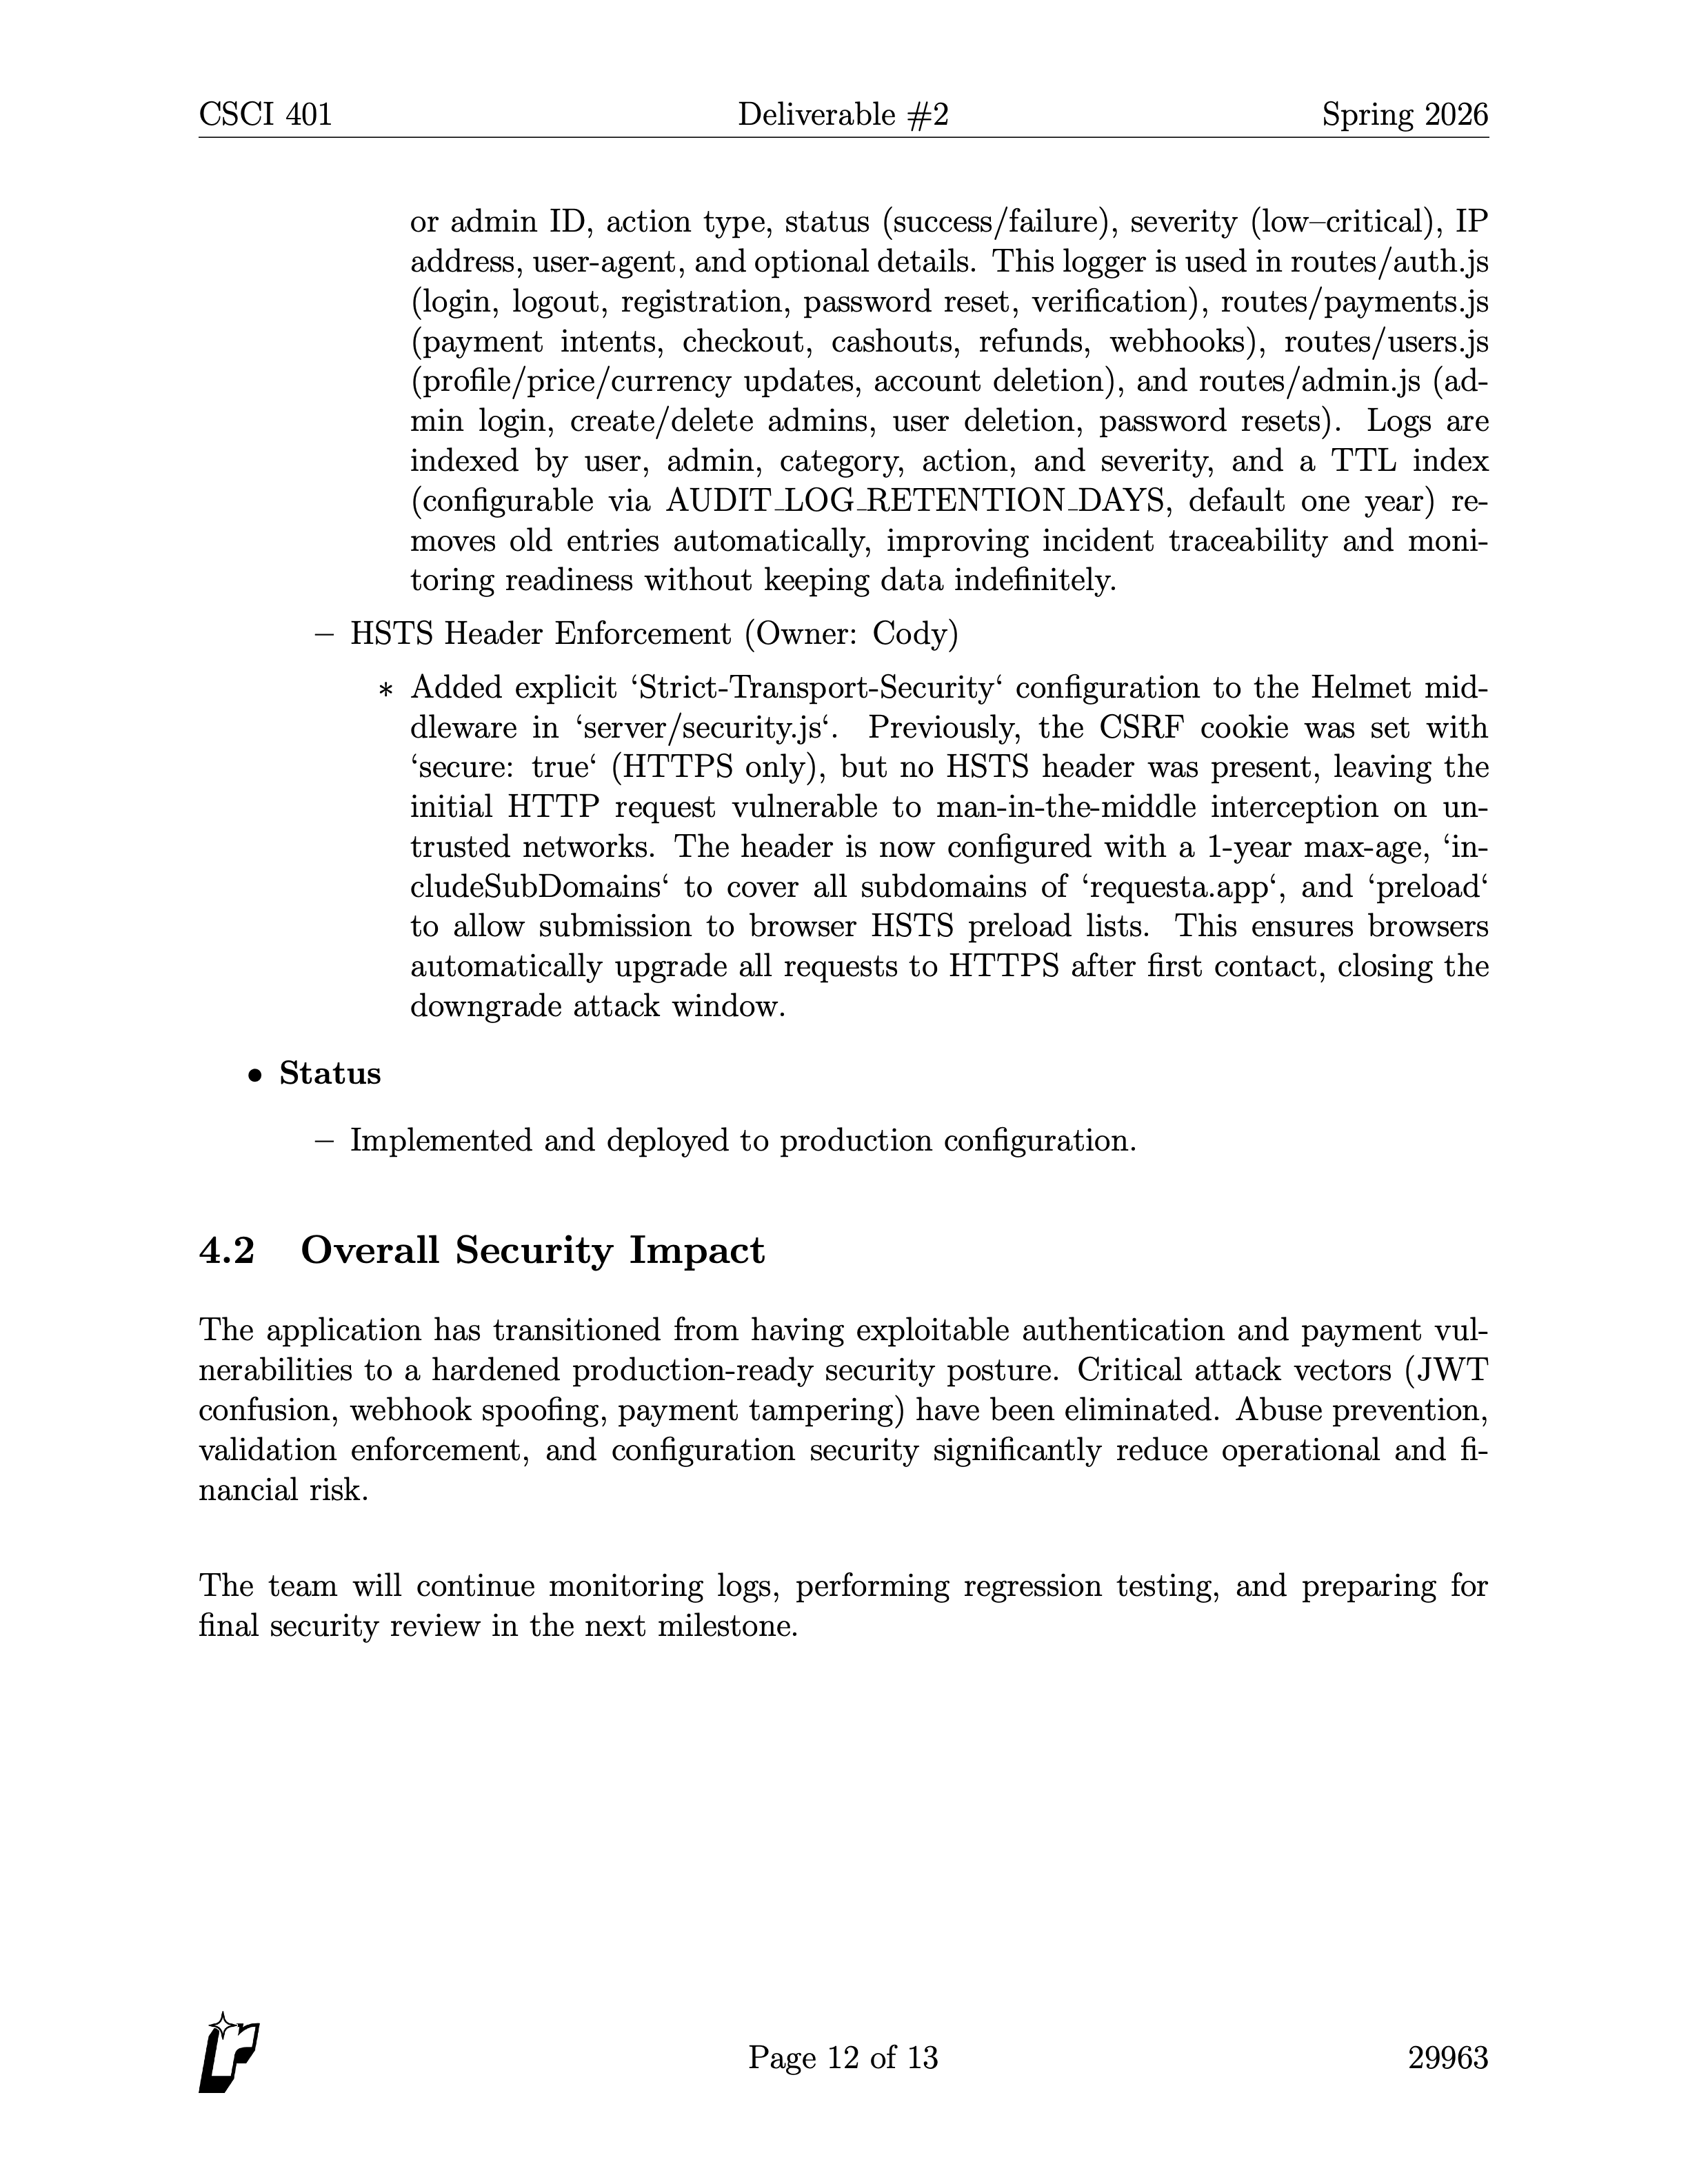
\includegraphics[width=0.48\textwidth,height=0.44\textheight,keepaspectratio]{images/deliverables/deliverable-3/Deliverable 3_12.png}
            \end{tabular}\end{figure}\clearpage

            \begin{figure}[H]\centering
            
\includegraphics[width=0.48\textwidth,height=0.44\textheight,keepaspectratio]{images/deliverables/deliverable-3/Deliverable 3_13.png}
            \end{figure}\clearpage

            \subsubsection{Deliverable 4}

            \begin{figure}[H]\centering\setlength{\tabcolsep}{4pt}
            \begin{tabular}{cc}
            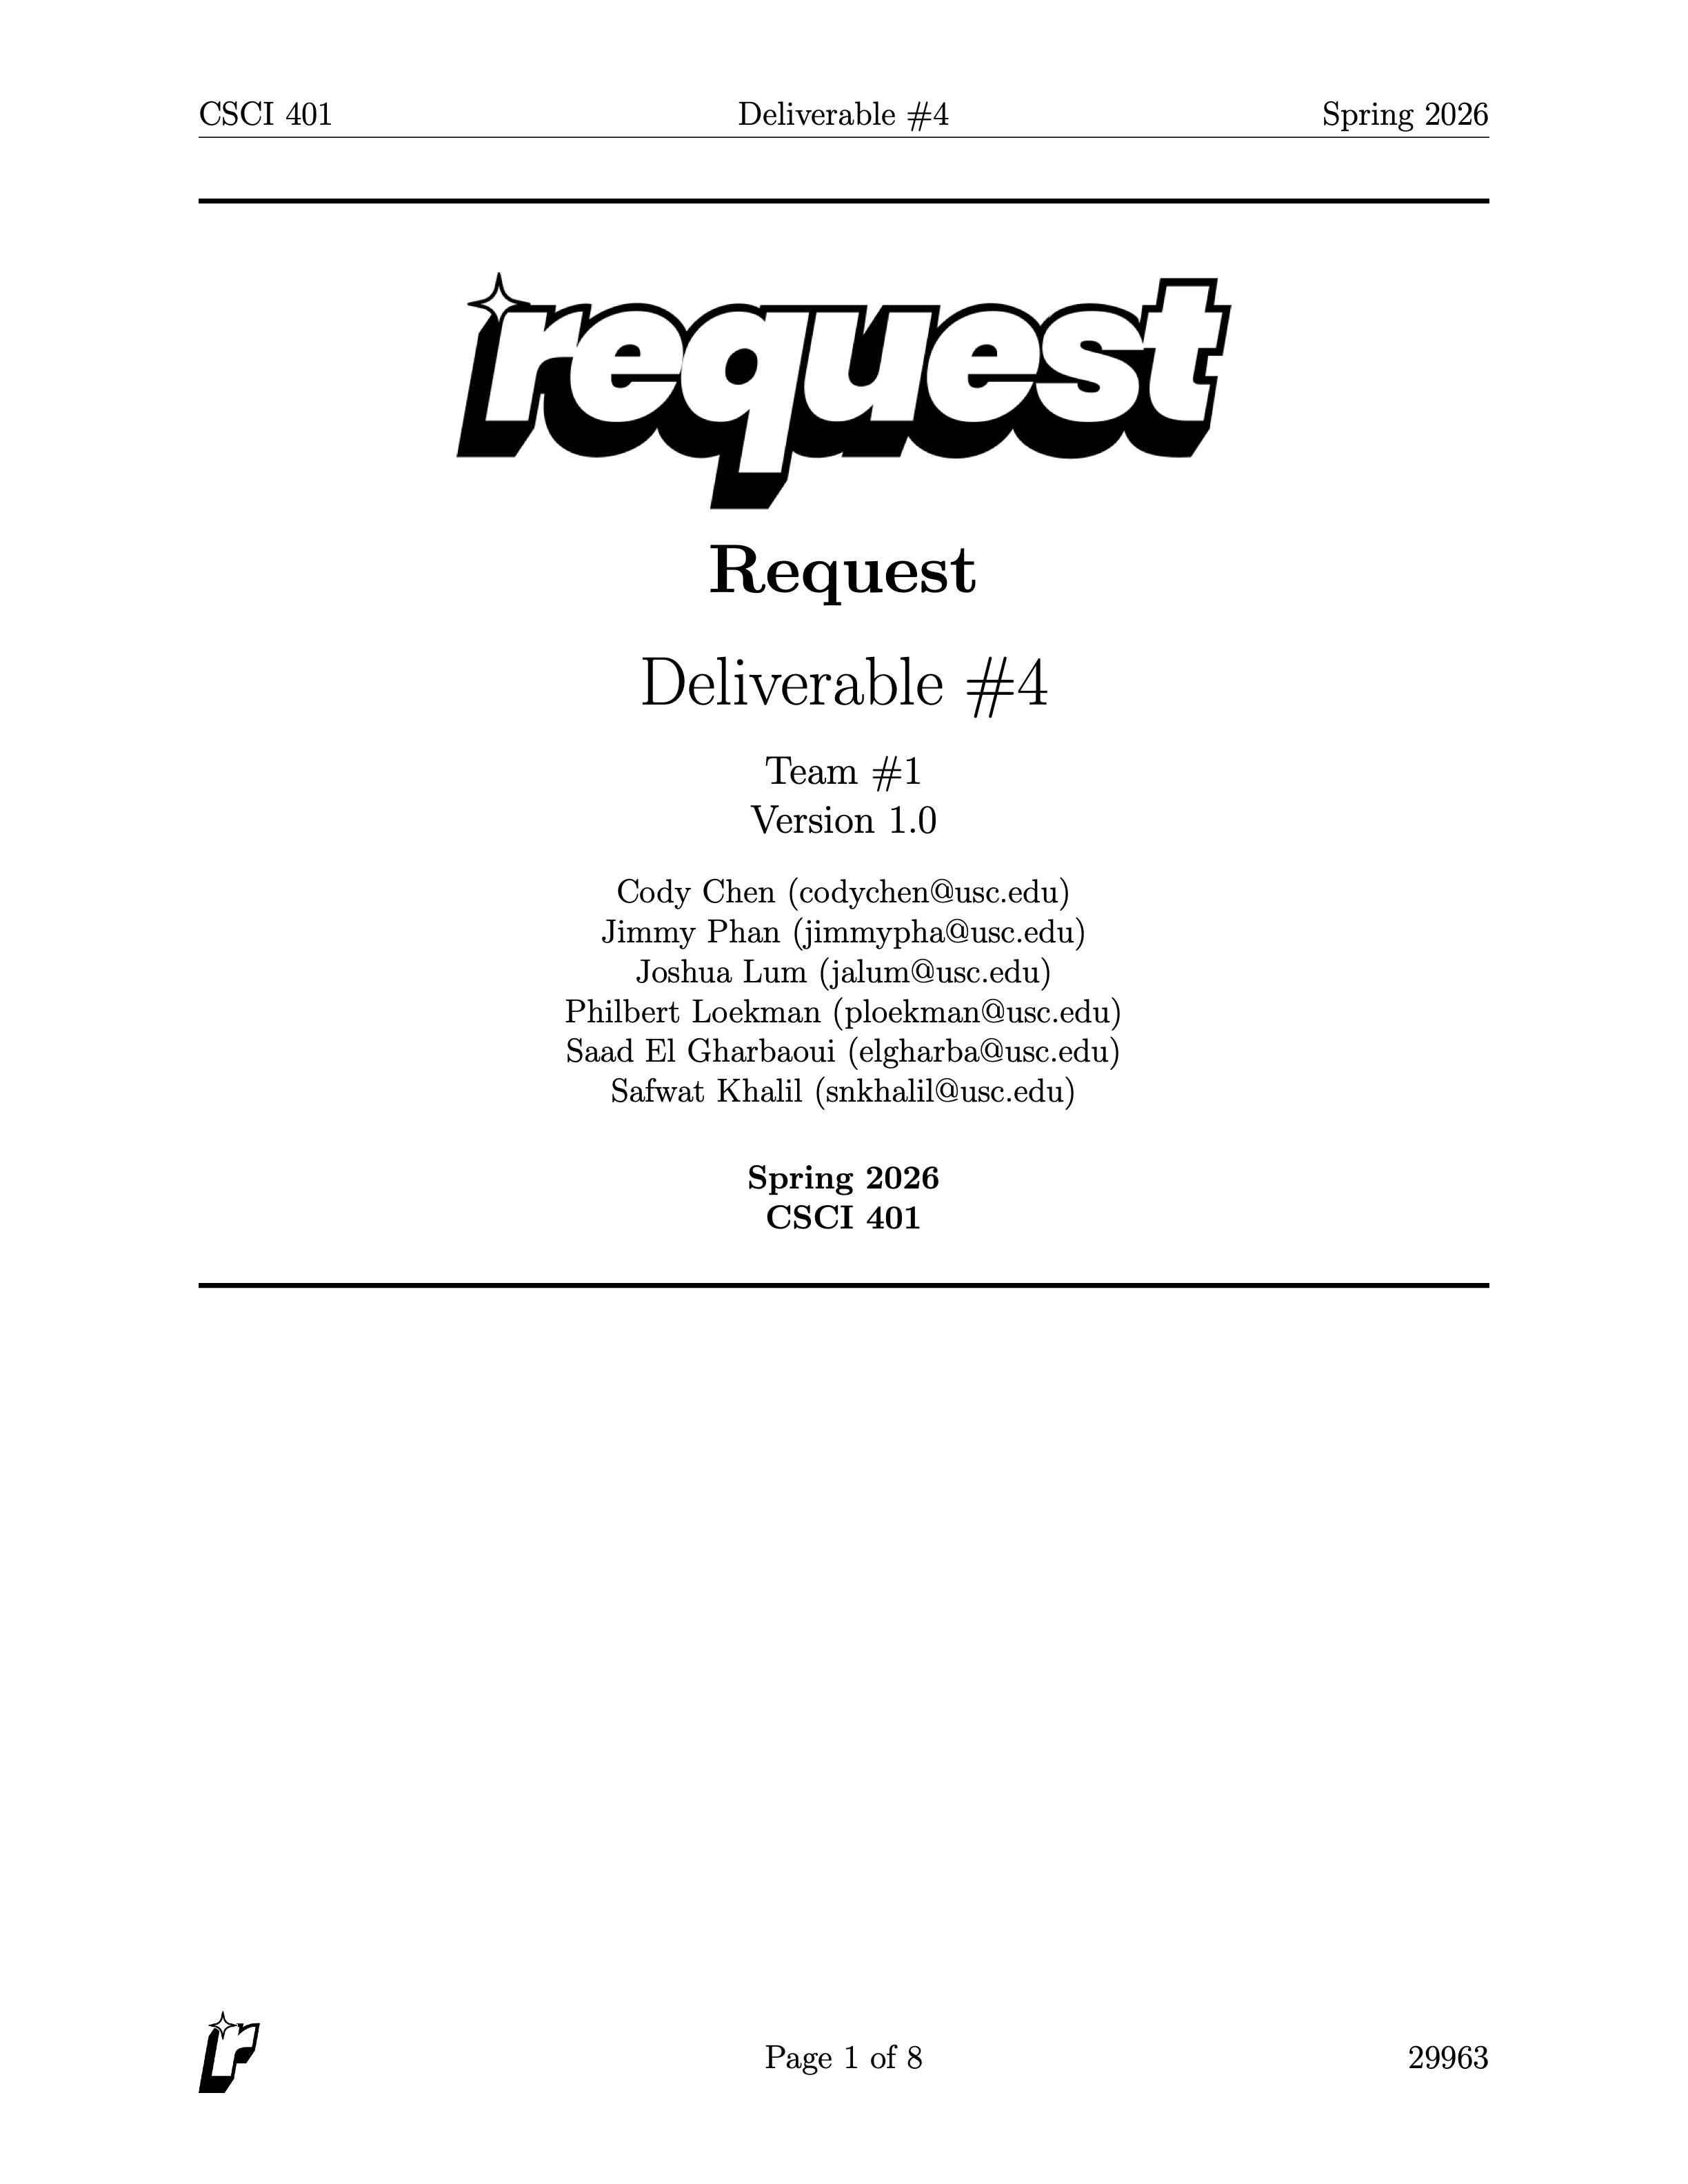
\includegraphics[width=0.48\textwidth,height=0.44\textheight,keepaspectratio]{images/deliverables/deliverable-4/Deliverable 4_1.png} &
            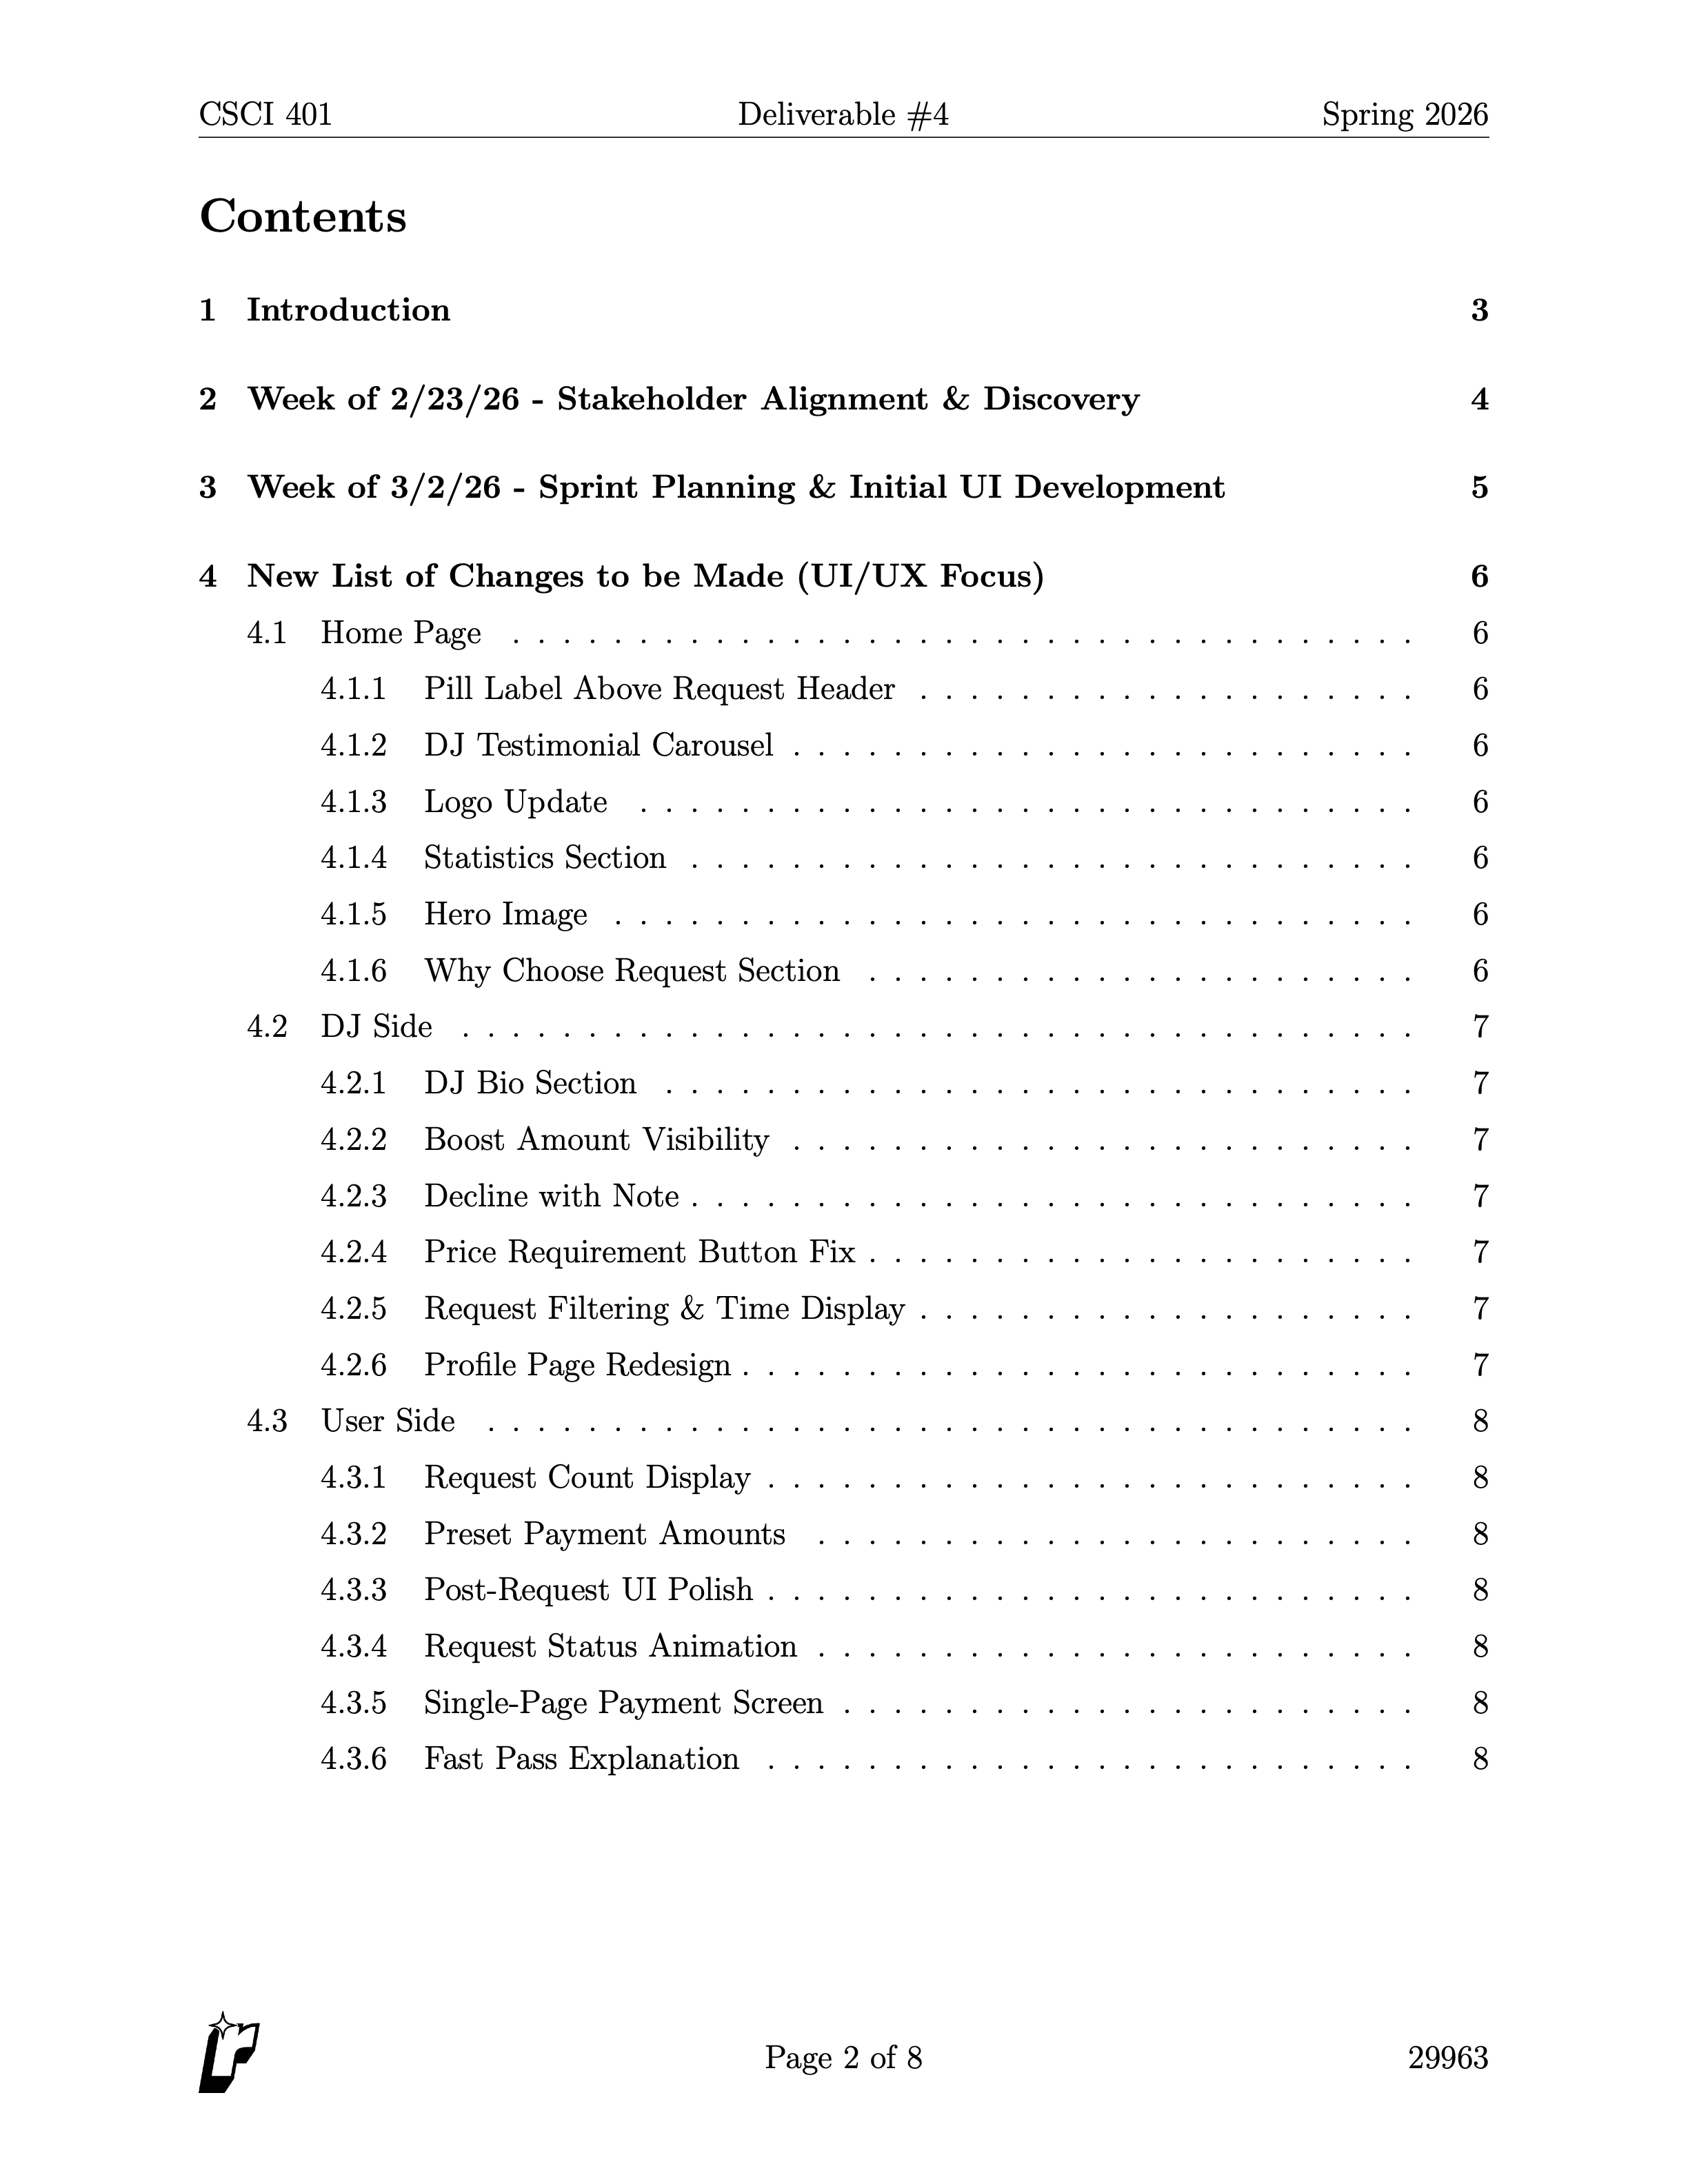
\includegraphics[width=0.48\textwidth,height=0.44\textheight,keepaspectratio]{images/deliverables/deliverable-4/Deliverable 4_2.png} \\[4pt]
            
\includegraphics[width=0.48\textwidth,height=0.44\textheight,keepaspectratio]{images/deliverables/deliverable-4/Deliverable 4_3.png} &
            
\includegraphics[width=0.48\textwidth,height=0.44\textheight,keepaspectratio]{images/deliverables/deliverable-4/Deliverable 4_4.png}
            \end{tabular}\end{figure}\clearpage

            \begin{figure}[H]\centering\setlength{\tabcolsep}{4pt}
            \begin{tabular}{cc}
            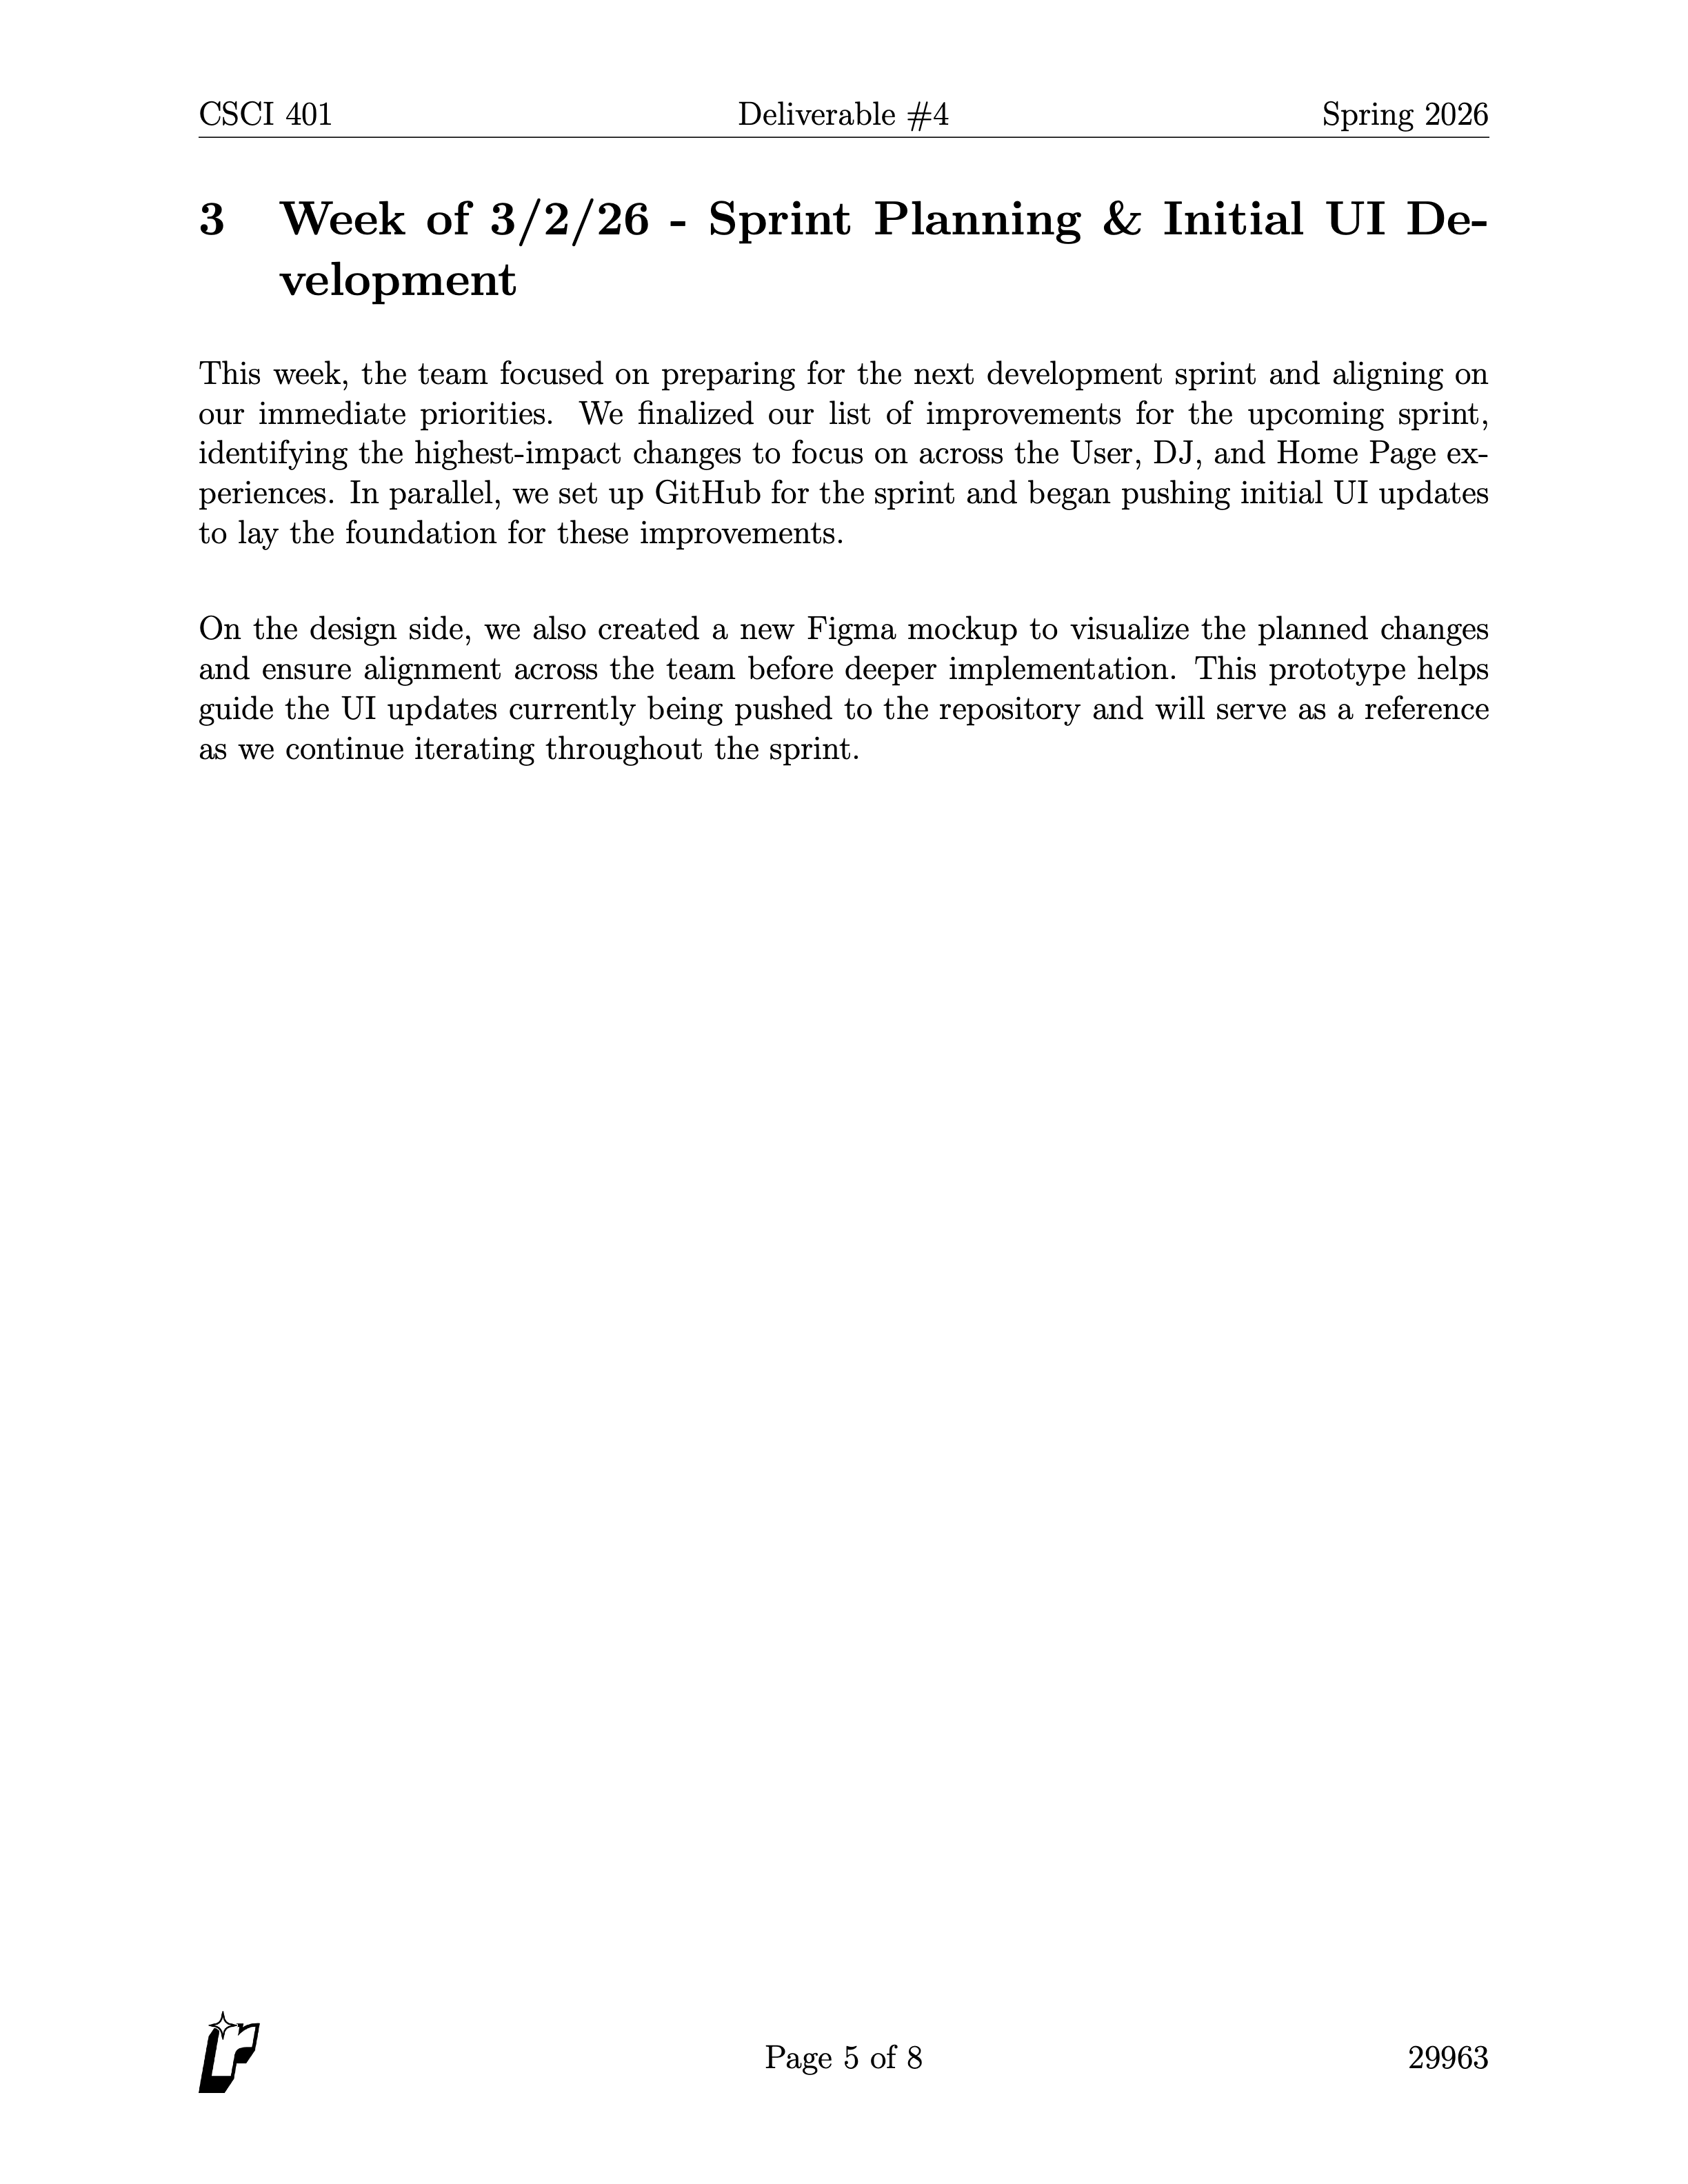
\includegraphics[width=0.48\textwidth,height=0.44\textheight,keepaspectratio]{images/deliverables/deliverable-4/Deliverable 4_5.png} &
            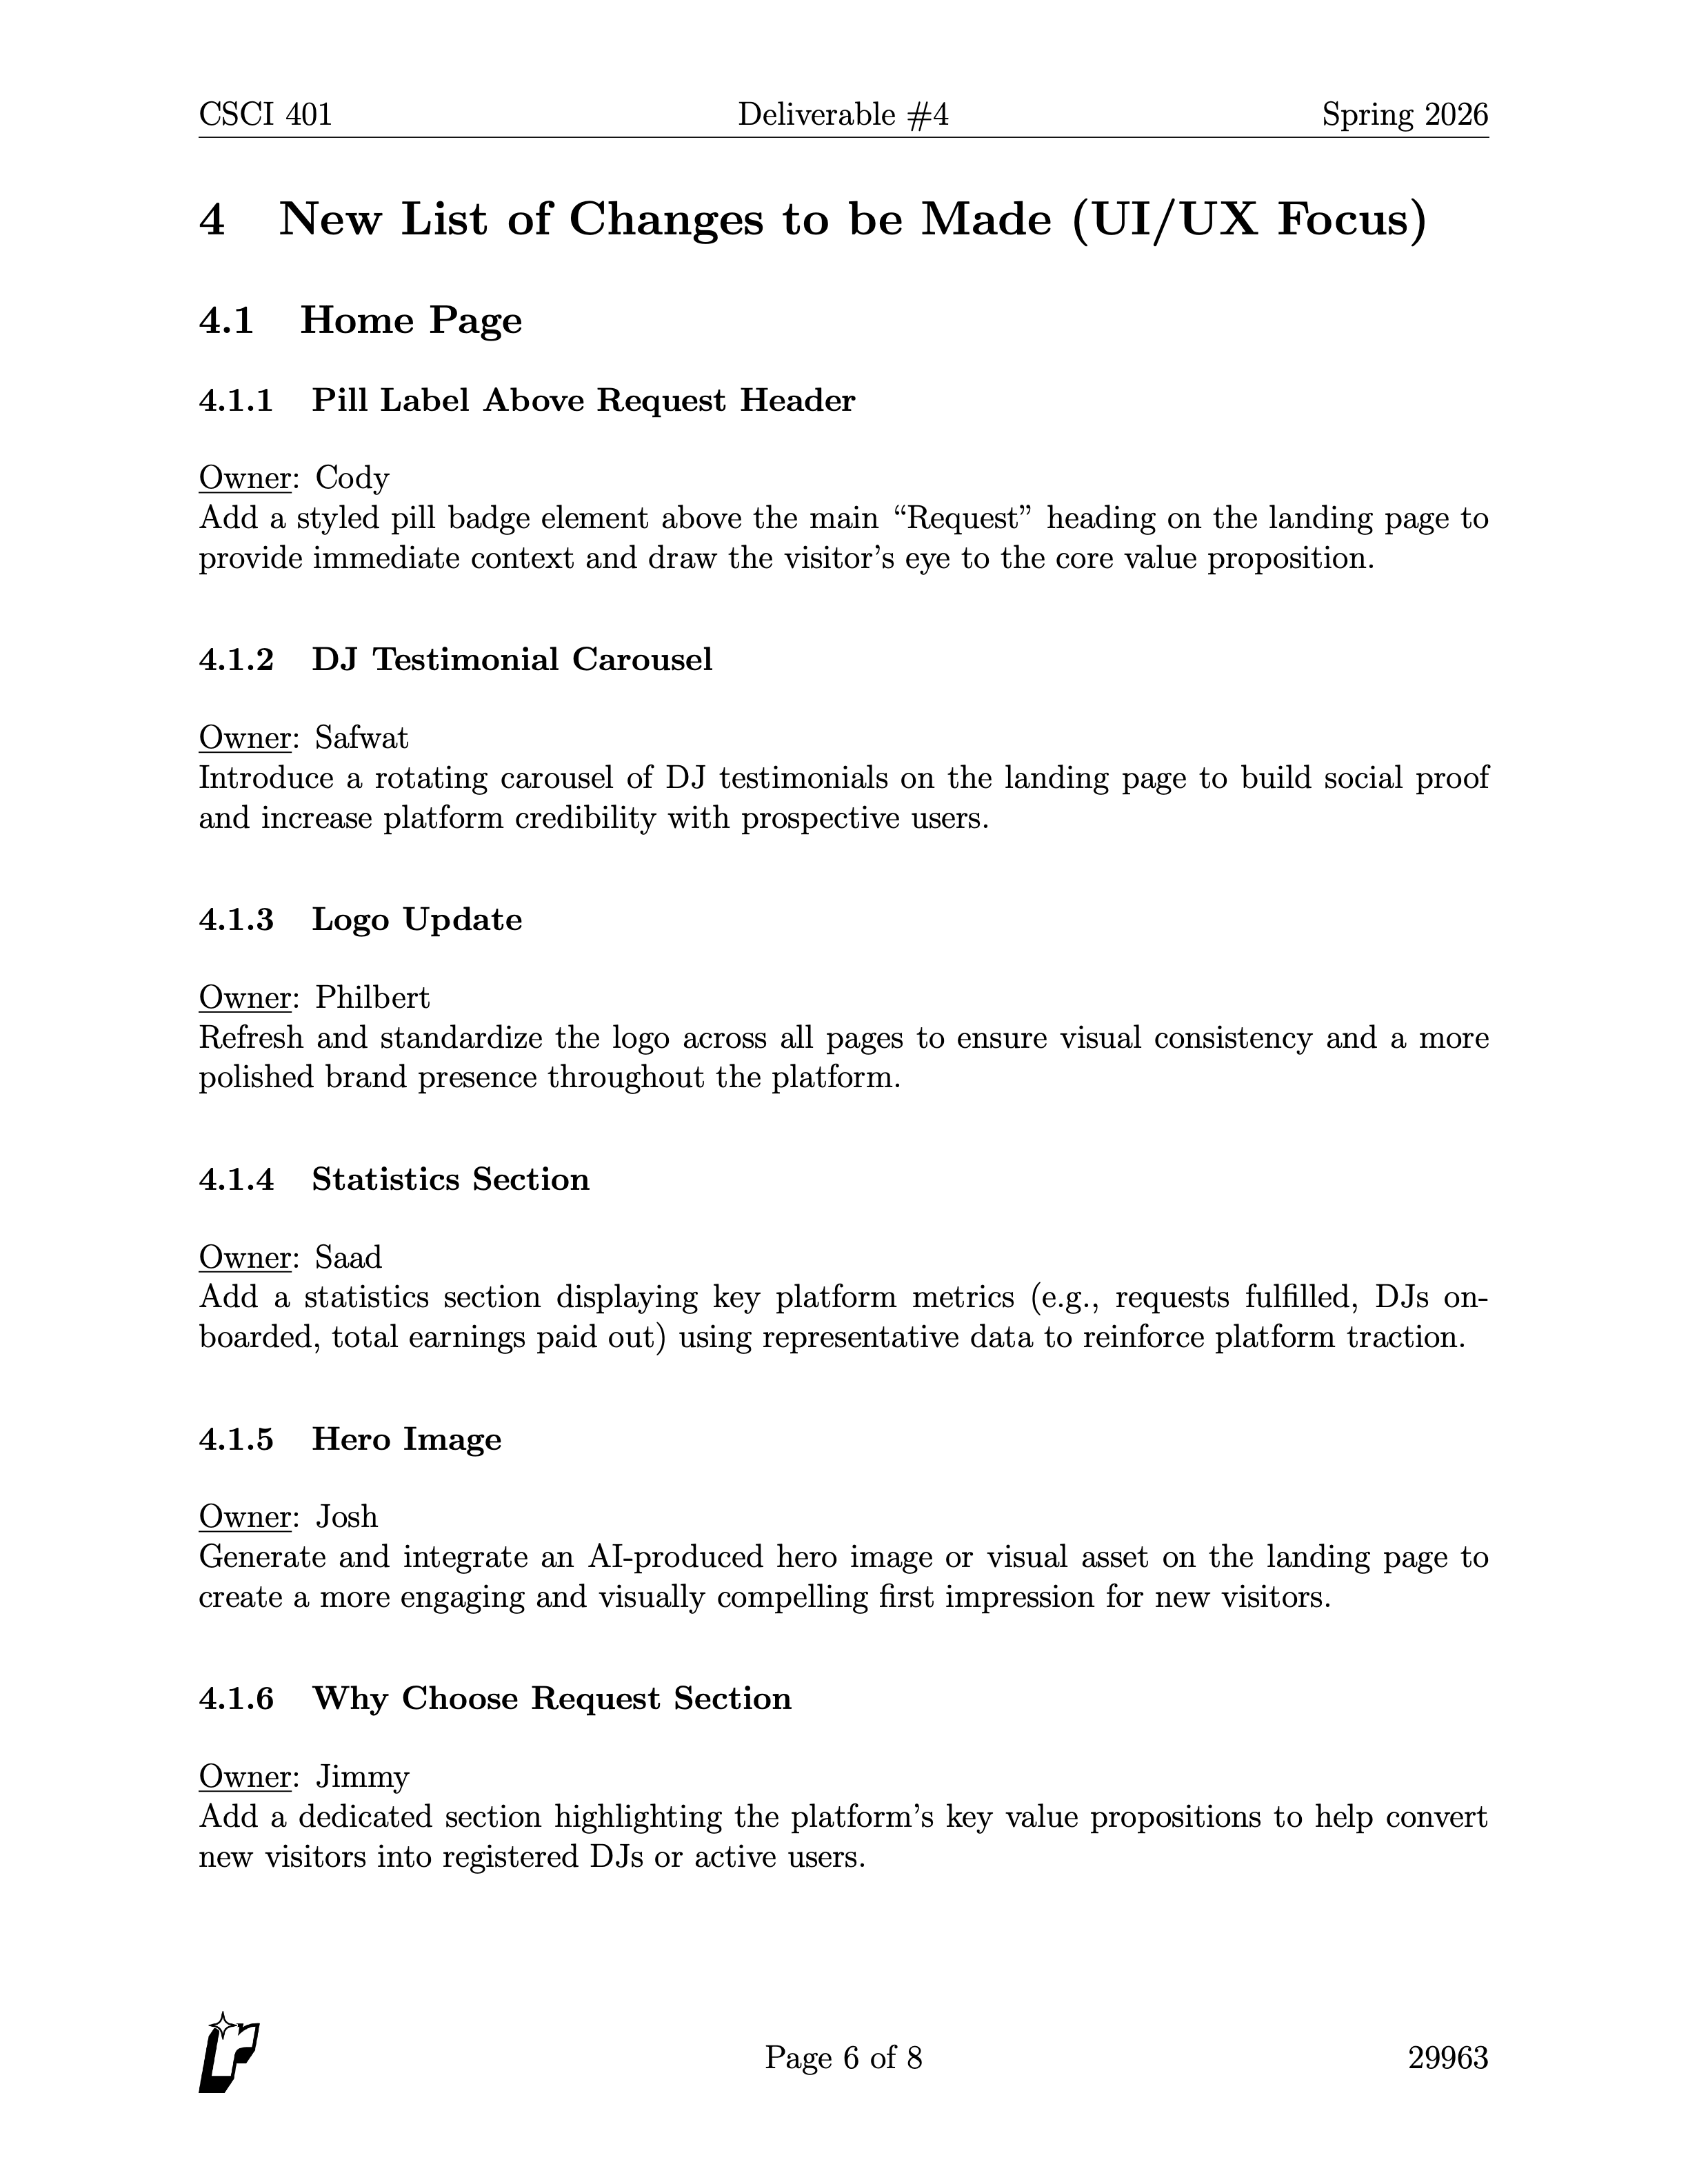
\includegraphics[width=0.48\textwidth,height=0.44\textheight,keepaspectratio]{images/deliverables/deliverable-4/Deliverable 4_6.png} \\[4pt]
            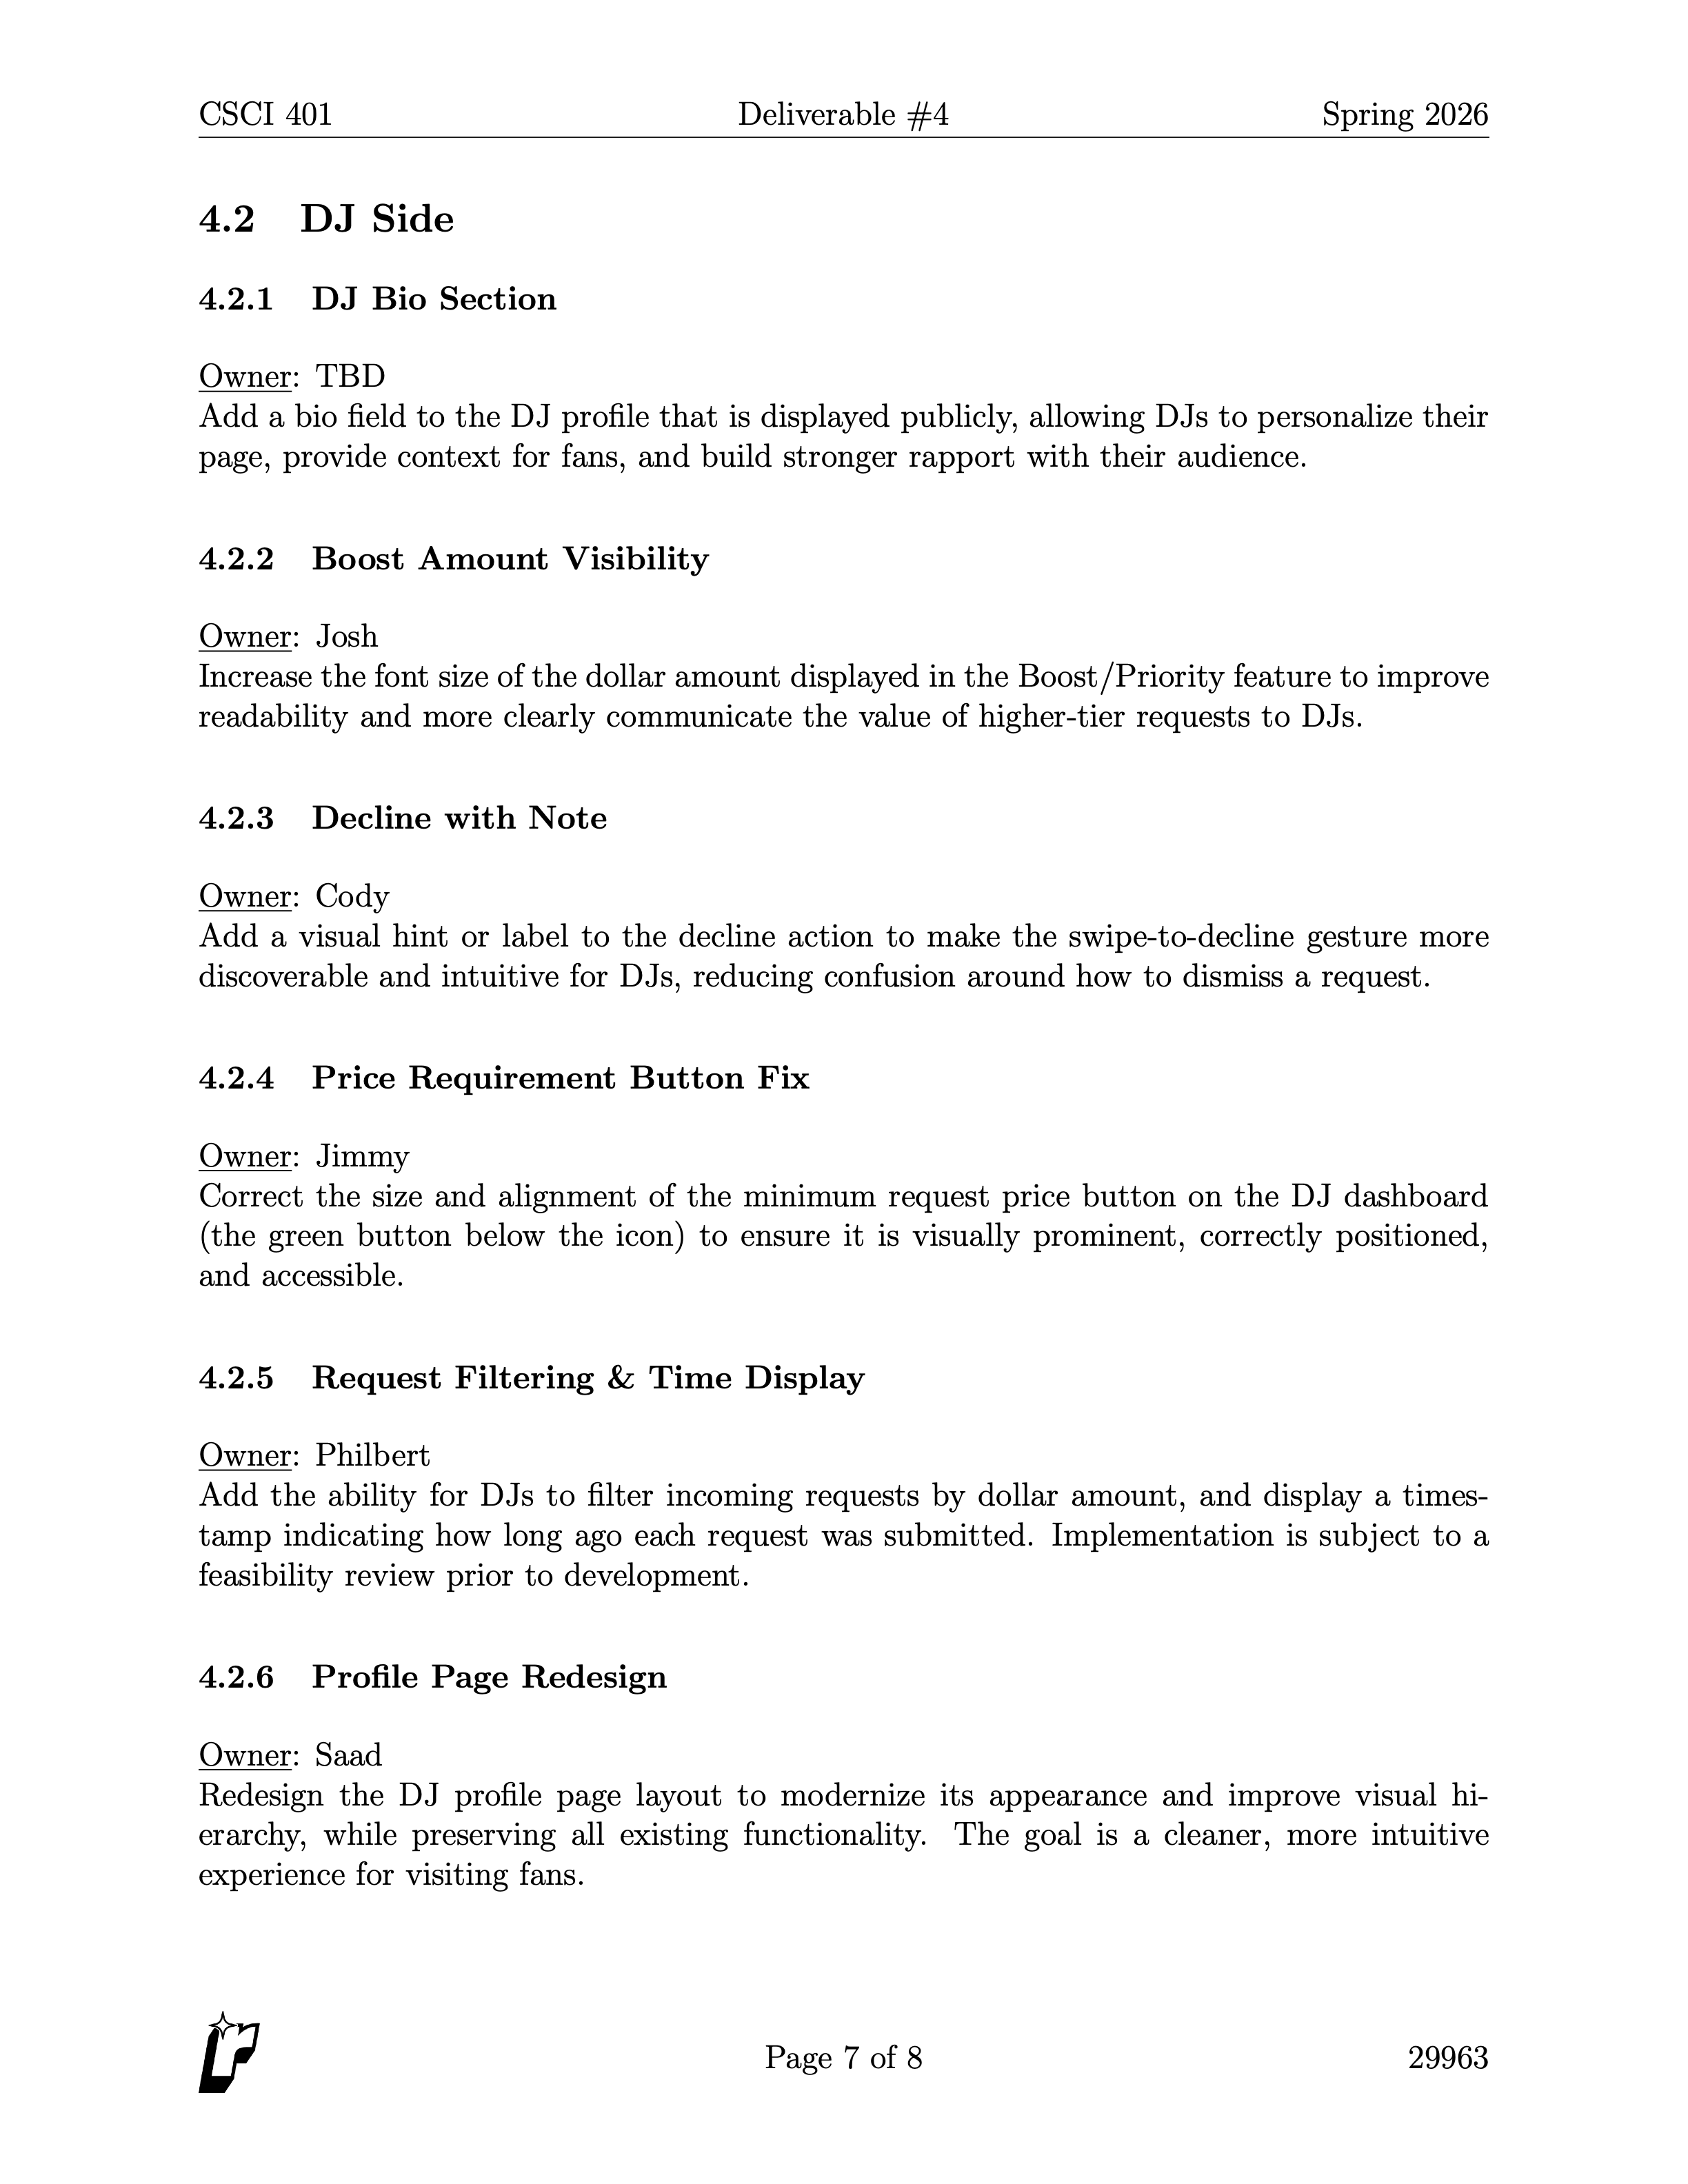
\includegraphics[width=0.48\textwidth,height=0.44\textheight,keepaspectratio]{images/deliverables/deliverable-4/Deliverable 4_7.png} &
            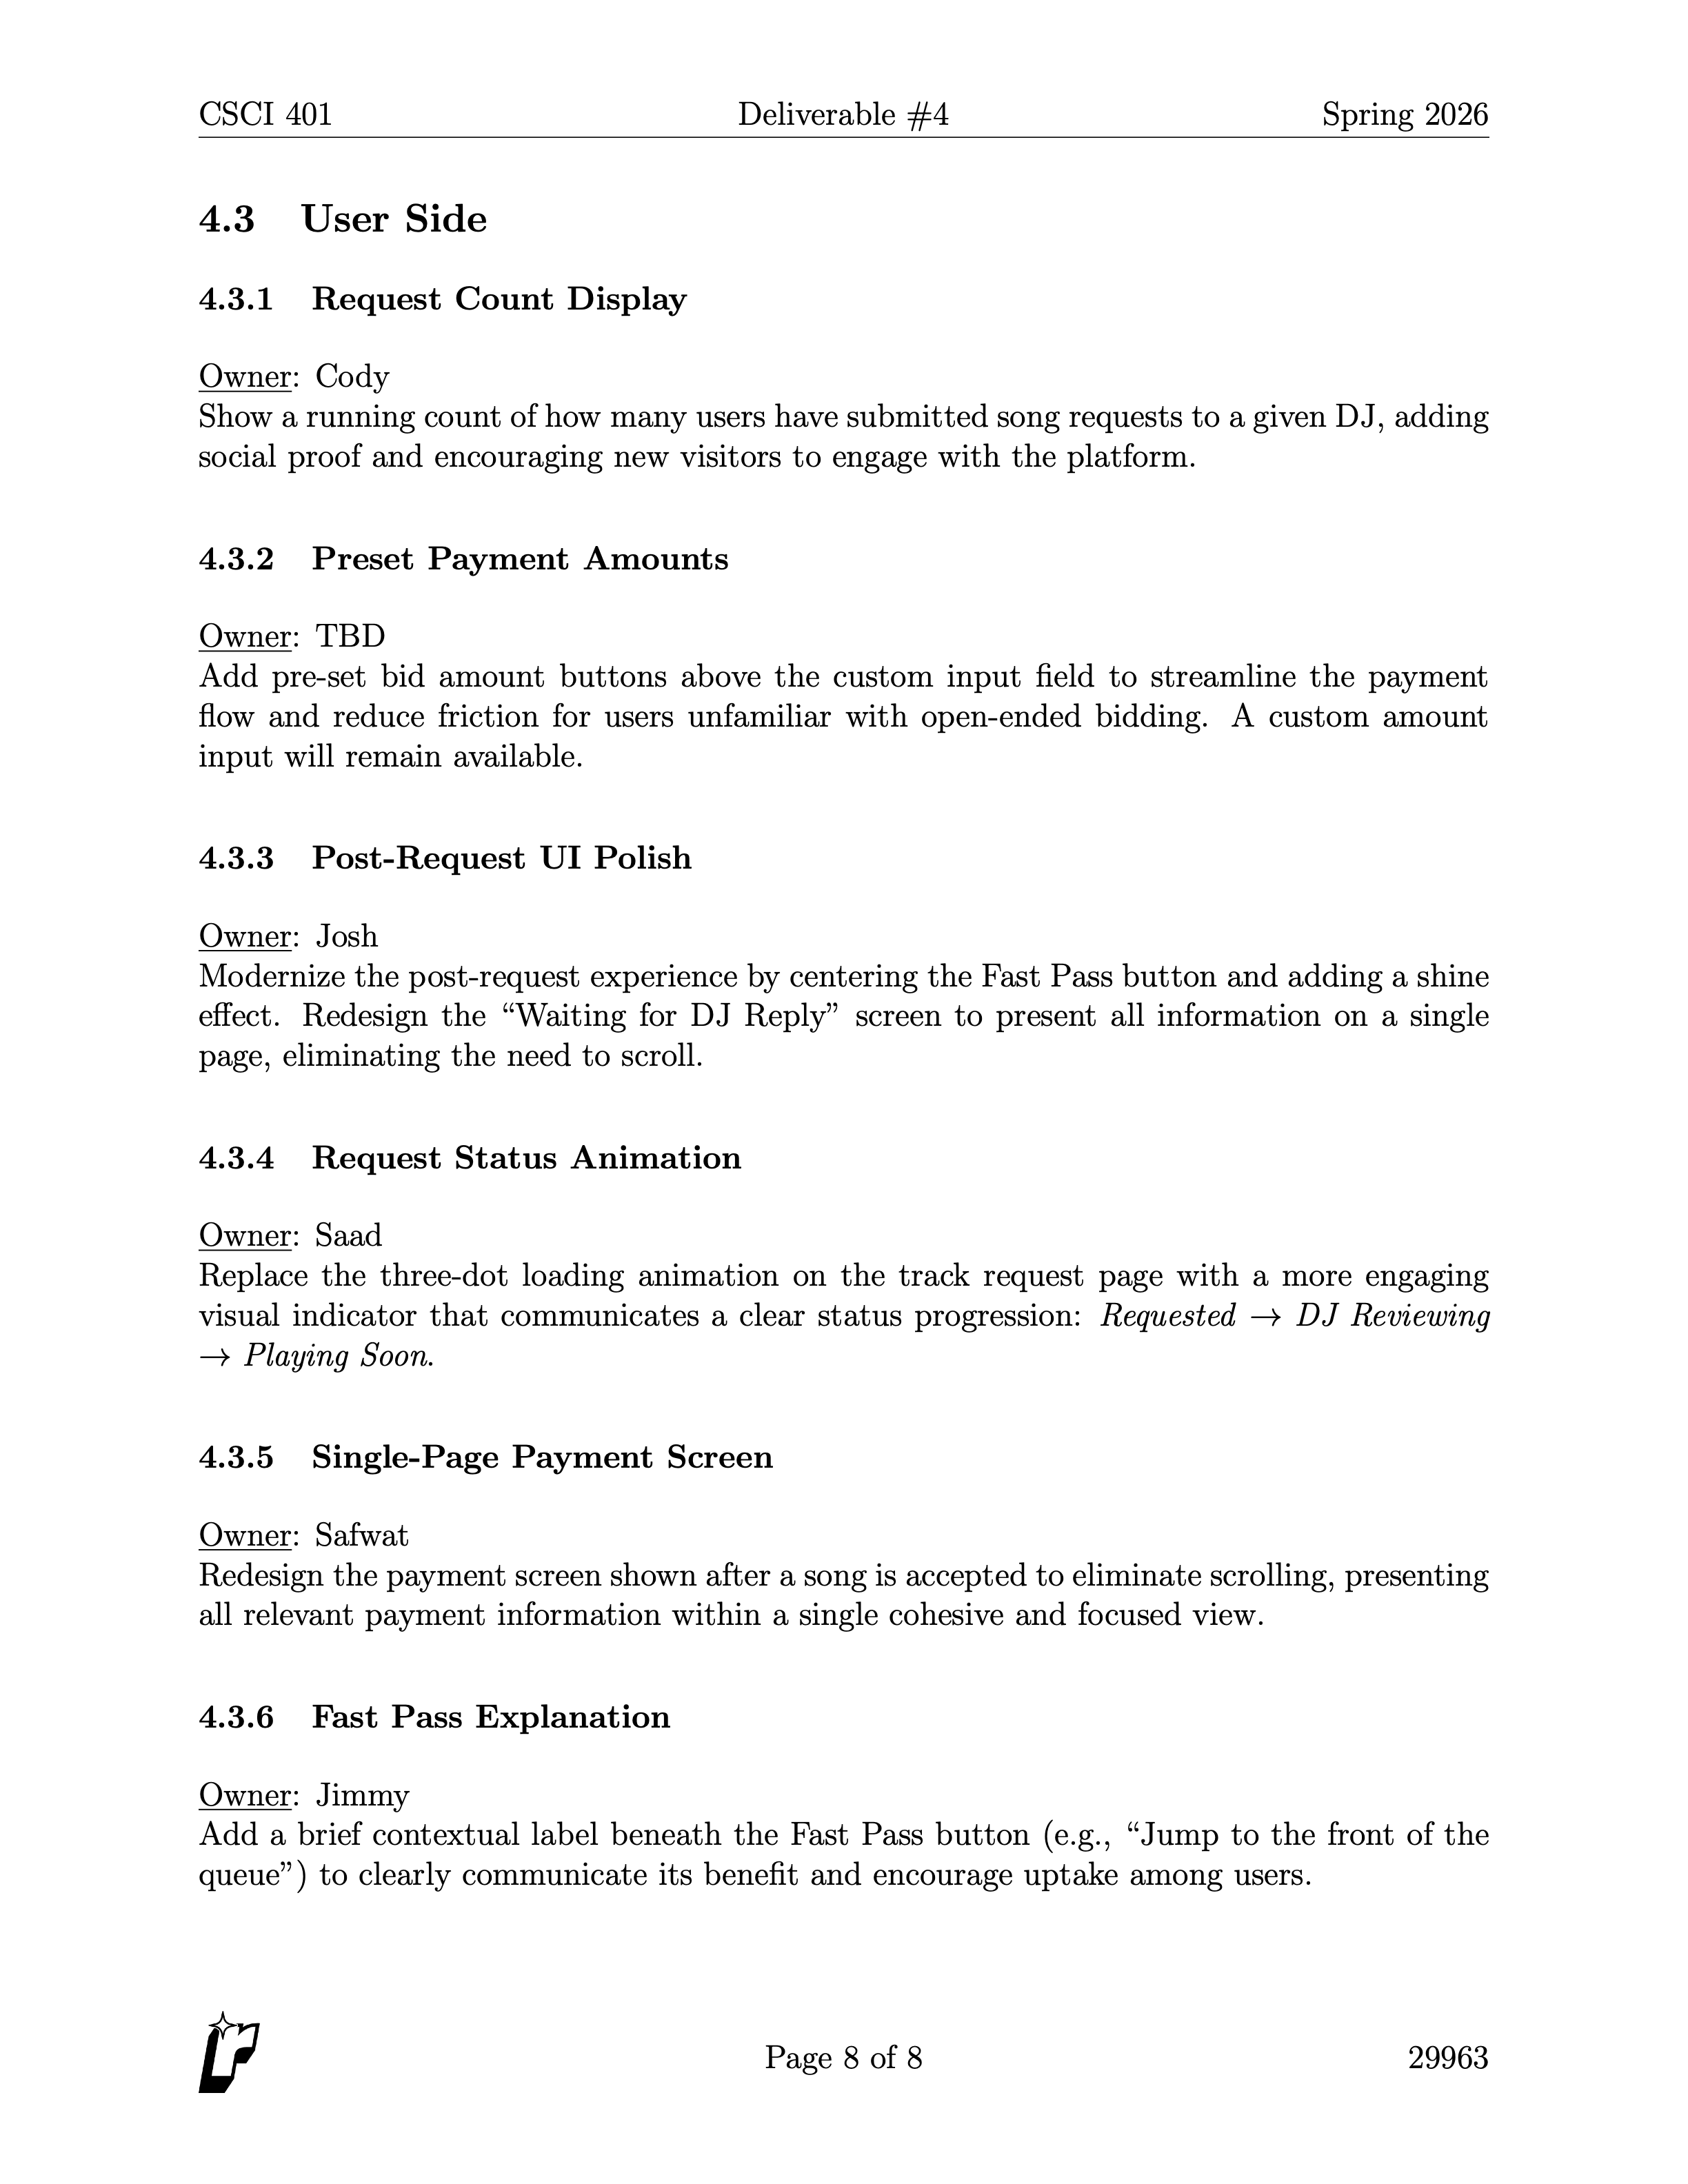
\includegraphics[width=0.48\textwidth,height=0.44\textheight,keepaspectratio]{images/deliverables/deliverable-4/Deliverable 4_8.png}
            \end{tabular}\end{figure}\clearpage

        \newpage
        \phantomsection\label{appendix:b}
        \subsection{Appendix B: Reading List \& Sources}

        % Book covers, reading logs, or other documentation

        \newpage
        \phantomsection\label{appendix:c}
        \subsection{Appendix C: Technical Description Before \& After}

        % Side-by-side or sequential comparison of drafts

        \newpage
        \phantomsection\label{appendix:d}
        \subsection{Appendix D: AI Coding Tool Videos \& Sources}

        % Links or screenshots of videos and resources used
        
        \newpage
        \newpage
        \phantomsection\label{appendix:e}
        \subsection{Appendix E: Pralumex Website Screenshots}

            \newpage
            \newpage
            \phantomsection\label{appendix:e1}
            \subsubsection{\texorpdfstring{E.1 --- Original Site (\href{https://old.pralumex.com}{old.pralumex.com})}{E.1 --- Original Site (old.pralumex.com)}}

            \begin{figure}[H]\centering
            
\includegraphics[width=\textwidth,height=0.46\textheight,keepaspectratio]{images/pralumex-website/old/1.png}\\[4pt]
            
\includegraphics[width=\textwidth,height=0.46\textheight,keepaspectratio]{images/pralumex-website/old/2.png}
            \end{figure}\clearpage
            \begin{figure}[H]\centering
            
\includegraphics[width=\textwidth,height=0.46\textheight,keepaspectratio]{images/pralumex-website/old/3.png}\\[4pt]
            
\includegraphics[width=\textwidth,height=0.46\textheight,keepaspectratio]{images/pralumex-website/old/4.png}
            \end{figure}\clearpage
            \begin{figure}[H]\centering
            
\includegraphics[width=\textwidth,height=0.46\textheight,keepaspectratio]{images/pralumex-website/old/5.png}
            \end{figure}\clearpage

            \newpage
            \phantomsection\label{appendix:e2}
            \subsubsection{\texorpdfstring{E.2 --- Current Site (\href{https://pralumex.com}{pralumex.com})}{E.2 --- Current Site (pralumex.com)}}

            \begin{figure}[H]\centering
            
\includegraphics[width=\textwidth,height=0.46\textheight,keepaspectratio]{images/pralumex-website/current/1.png}\\[4pt]
            
\includegraphics[width=\textwidth,height=0.46\textheight,keepaspectratio]{images/pralumex-website/current/2.png}
            \end{figure}\clearpage
            \begin{figure}[H]\centering
            
\includegraphics[width=\textwidth,height=0.46\textheight,keepaspectratio]{images/pralumex-website/current/3.png}\\[4pt]
            
\includegraphics[width=\textwidth,height=0.46\textheight,keepaspectratio]{images/pralumex-website/current/4.png}
            \end{figure}\clearpage
            \begin{figure}[H]\centering
            
\includegraphics[width=\textwidth,height=0.46\textheight,keepaspectratio]{images/pralumex-website/current/5.png}\\[4pt]
            
\includegraphics[width=\textwidth,height=0.46\textheight,keepaspectratio]{images/pralumex-website/current/6.png}
            \end{figure}\clearpage
            \begin{figure}[H]\centering
            
\includegraphics[width=\textwidth,height=0.46\textheight,keepaspectratio]{images/pralumex-website/current/7.png}\\[4pt]
            
\includegraphics[width=\textwidth,height=0.46\textheight,keepaspectratio]{images/pralumex-website/current/8.png}
            \end{figure}\clearpage
            \begin{figure}[H]\centering
            
\includegraphics[width=\textwidth,height=0.46\textheight,keepaspectratio]{images/pralumex-website/current/9.png}\\[4pt]
            
\includegraphics[width=\textwidth,height=0.46\textheight,keepaspectratio]{images/pralumex-website/current/10.png}
            \end{figure}\clearpage
            \begin{figure}[H]\centering
            
\includegraphics[width=\textwidth,height=0.46\textheight,keepaspectratio]{images/pralumex-website/current/11.png}\\[4pt]
            
\includegraphics[width=\textwidth,height=0.46\textheight,keepaspectratio]{images/pralumex-website/current/12.png}
            \end{figure}\clearpage
            \begin{figure}[H]\centering
            
\includegraphics[width=\textwidth,height=0.46\textheight,keepaspectratio]{images/pralumex-website/current/13.png}\\[4pt]
            
\includegraphics[width=\textwidth,height=0.46\textheight,keepaspectratio]{images/pralumex-website/current/14.png}
            \end{figure}\clearpage
            \begin{figure}[H]\centering
            
\includegraphics[width=\textwidth,height=0.46\textheight,keepaspectratio]{images/pralumex-website/current/15.png}
            \end{figure}\clearpage

            \newpage
            \phantomsection\label{appendix:e3}
            \subsubsection{\texorpdfstring{E.3 --- Beta Site (\href{https://beta.pralumex.com}{beta.pralumex.com})}{E.3 --- Beta Site (beta.pralumex.com)}}

            \begin{figure}[H]\centering
            
\includegraphics[width=\textwidth,height=0.46\textheight,keepaspectratio]{images/pralumex-website/beta/1.png}\\[4pt]
            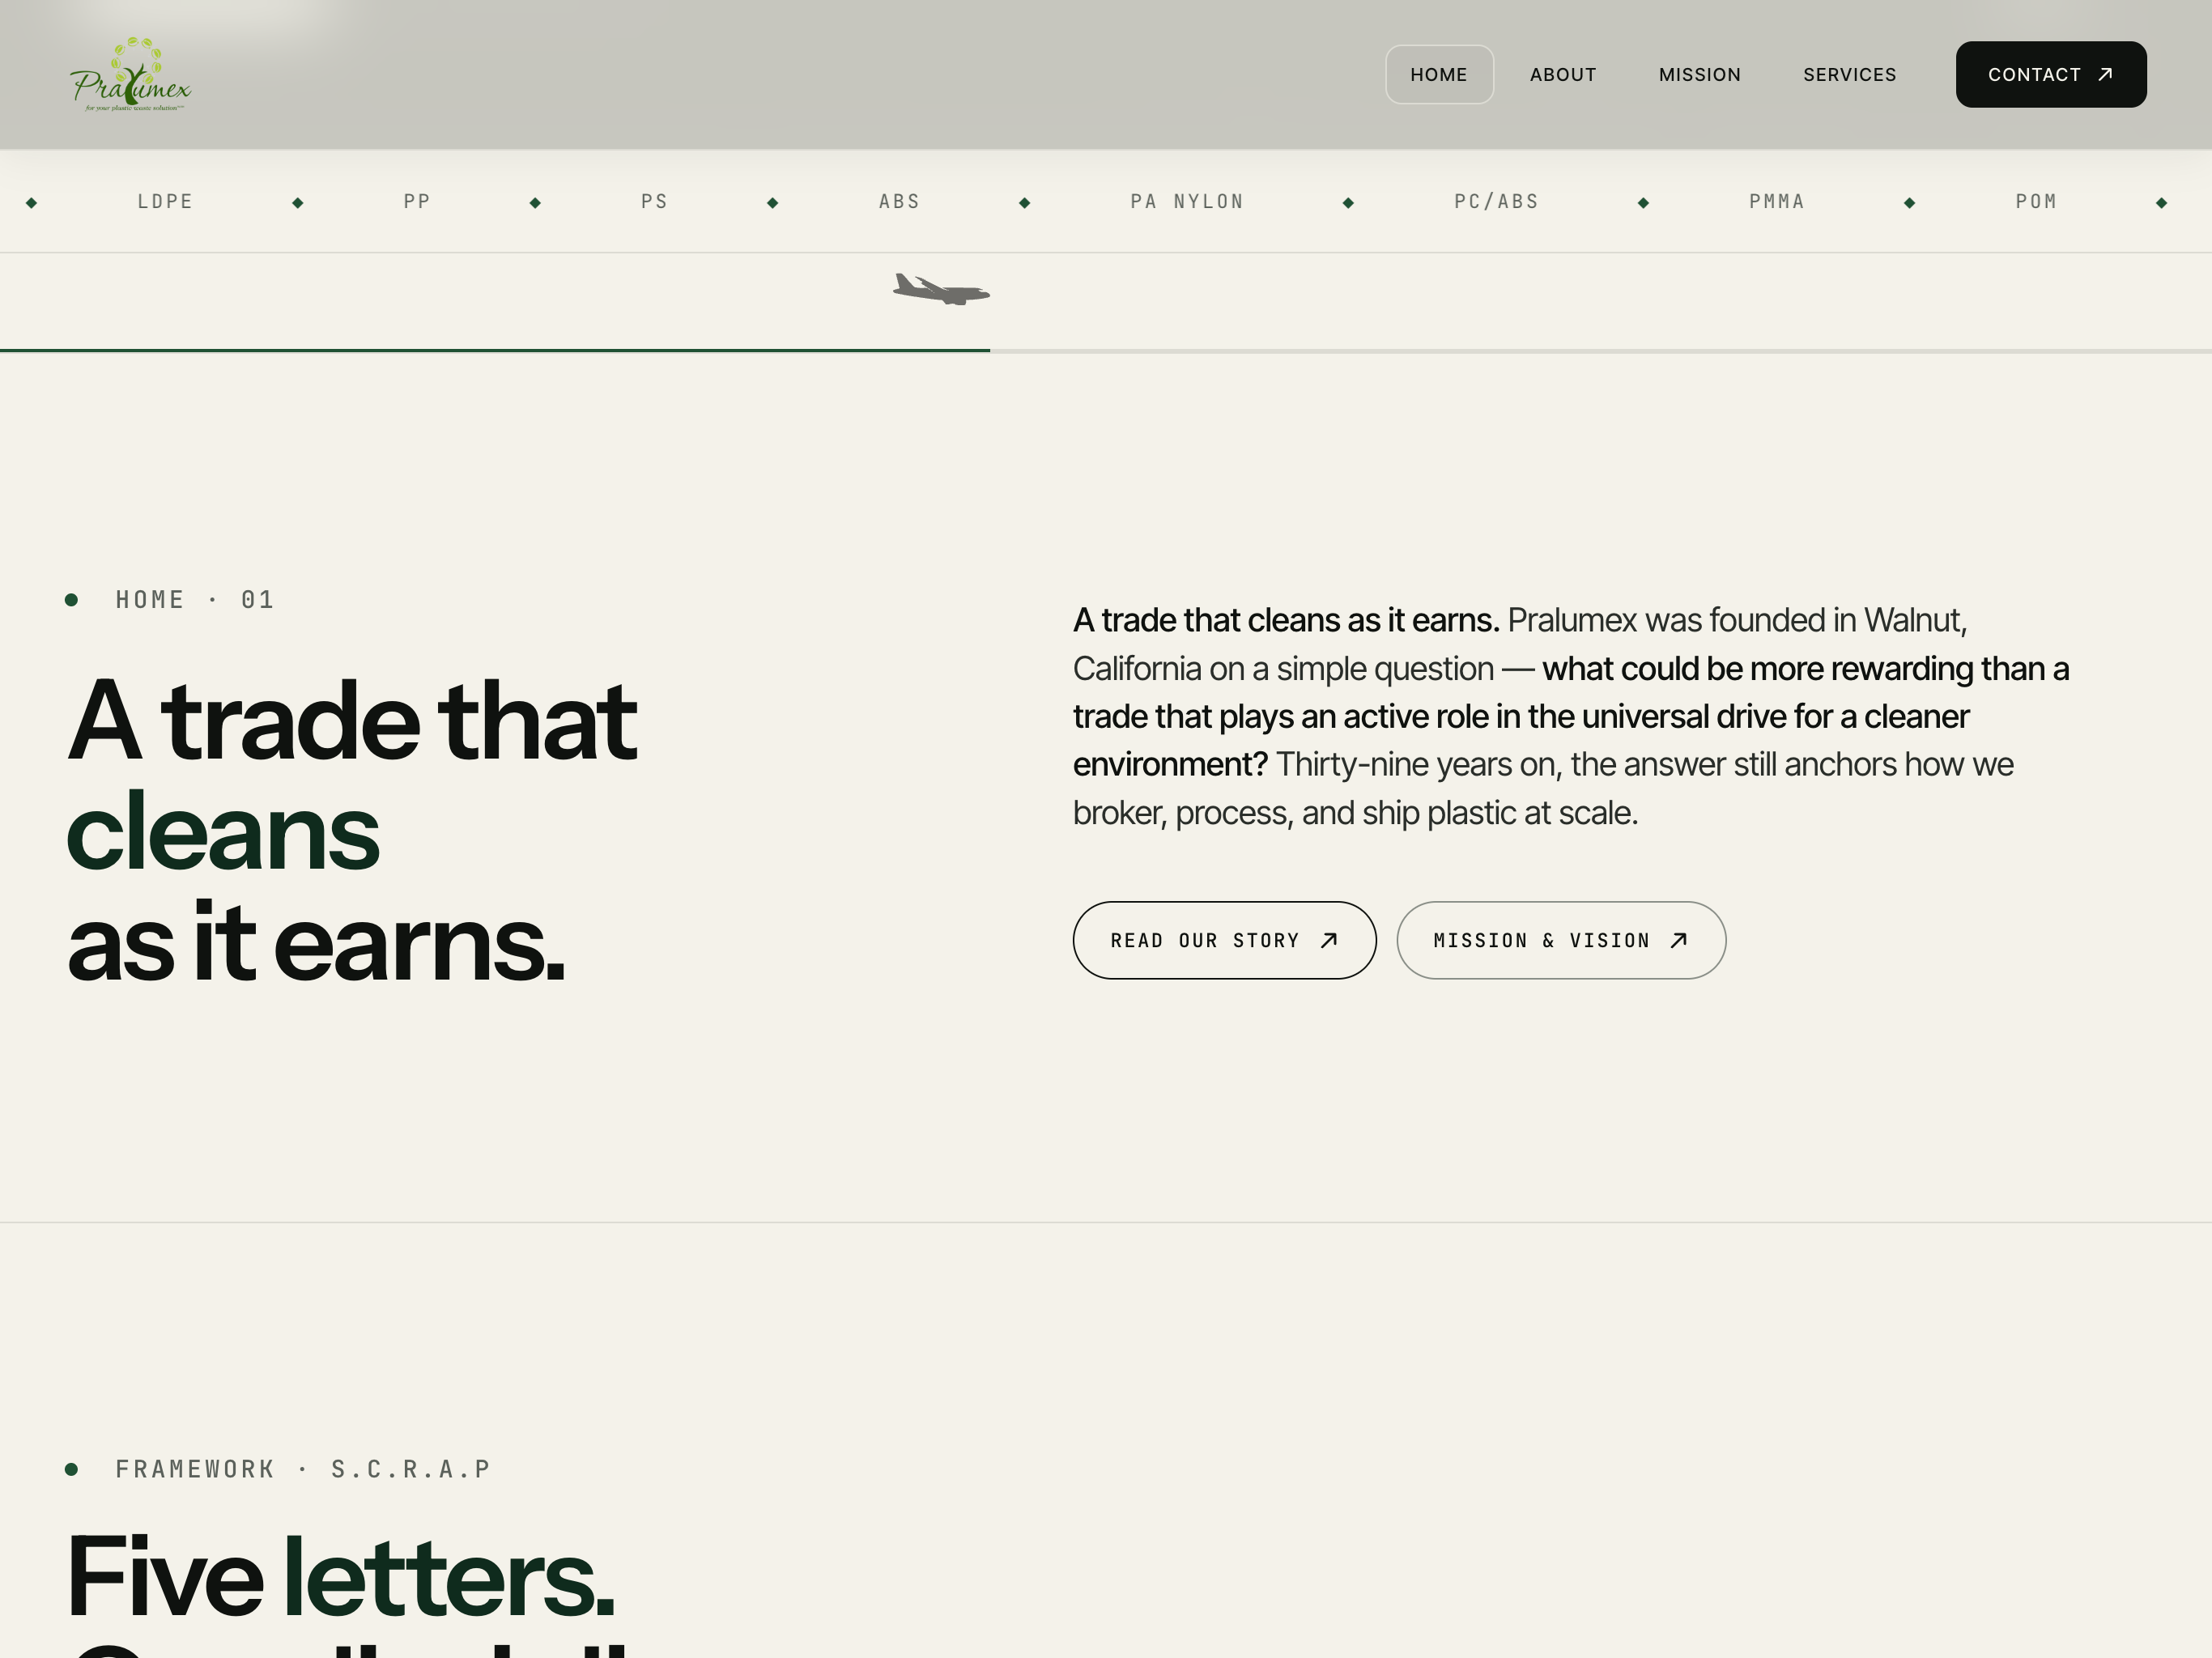
\includegraphics[width=\textwidth,height=0.46\textheight,keepaspectratio]{images/pralumex-website/beta/2.png}
            \end{figure}\clearpage
            \begin{figure}[H]\centering
            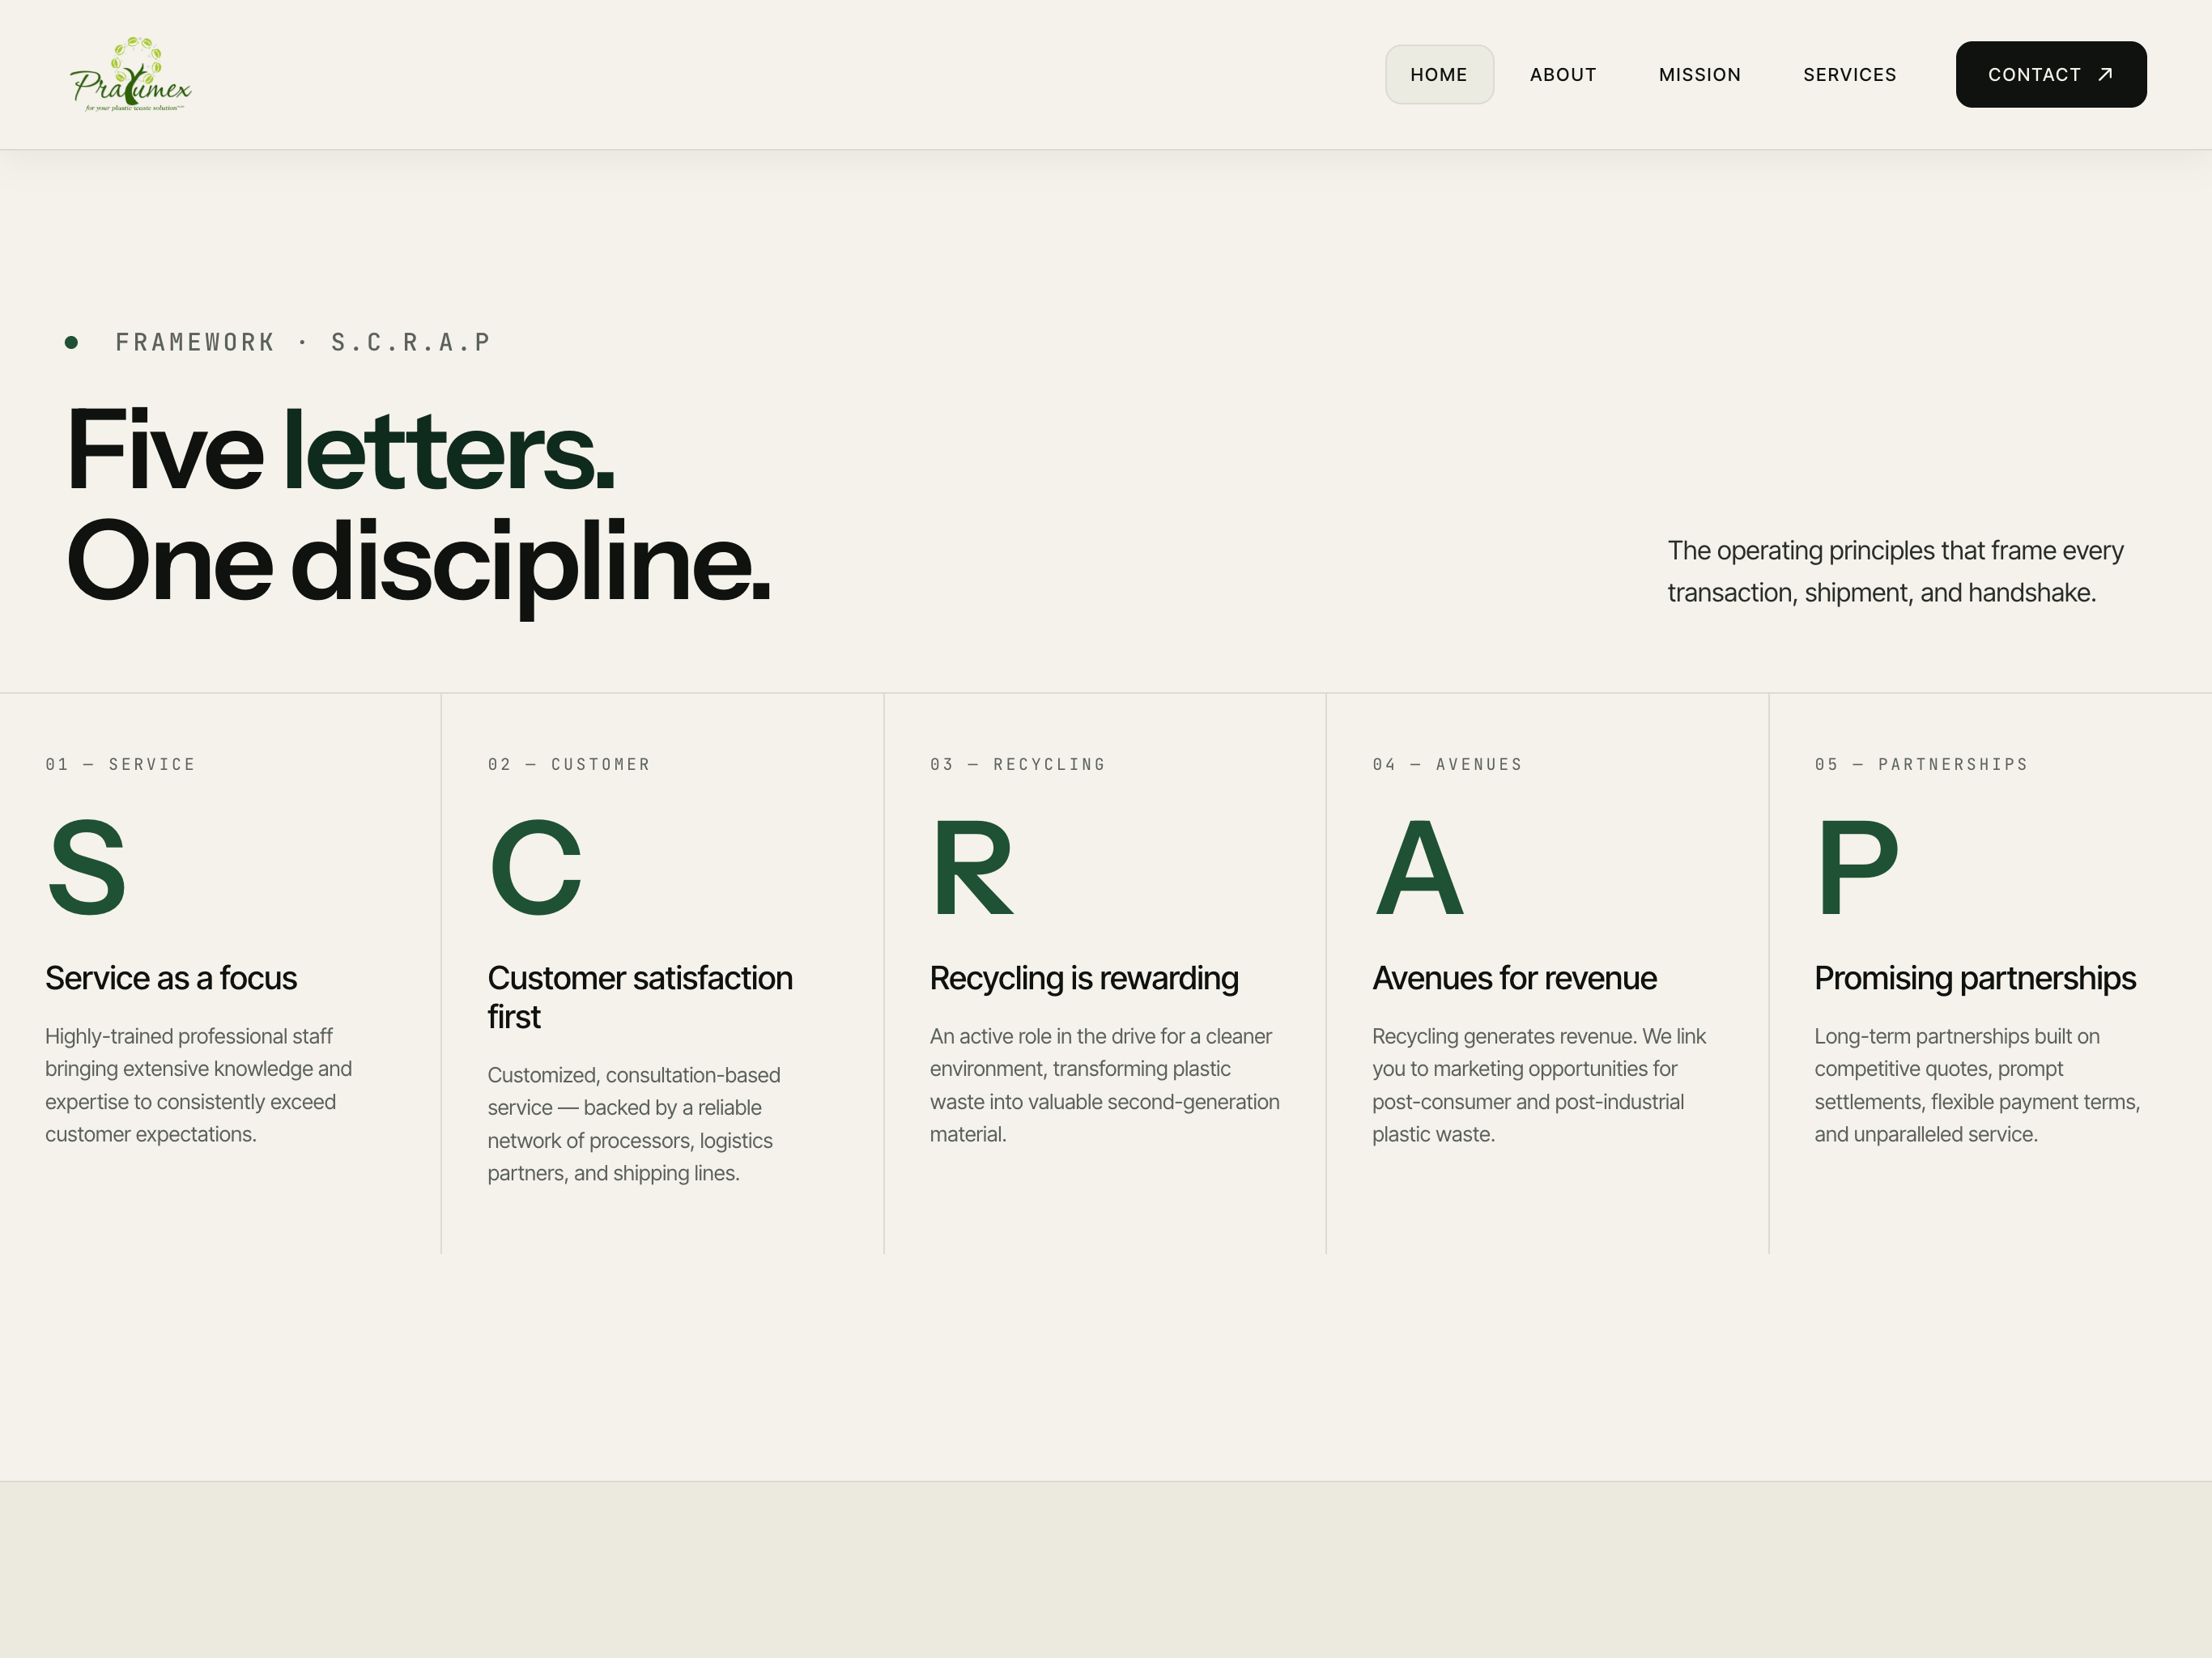
\includegraphics[width=\textwidth,height=0.46\textheight,keepaspectratio]{images/pralumex-website/beta/3.png}\\[4pt]
            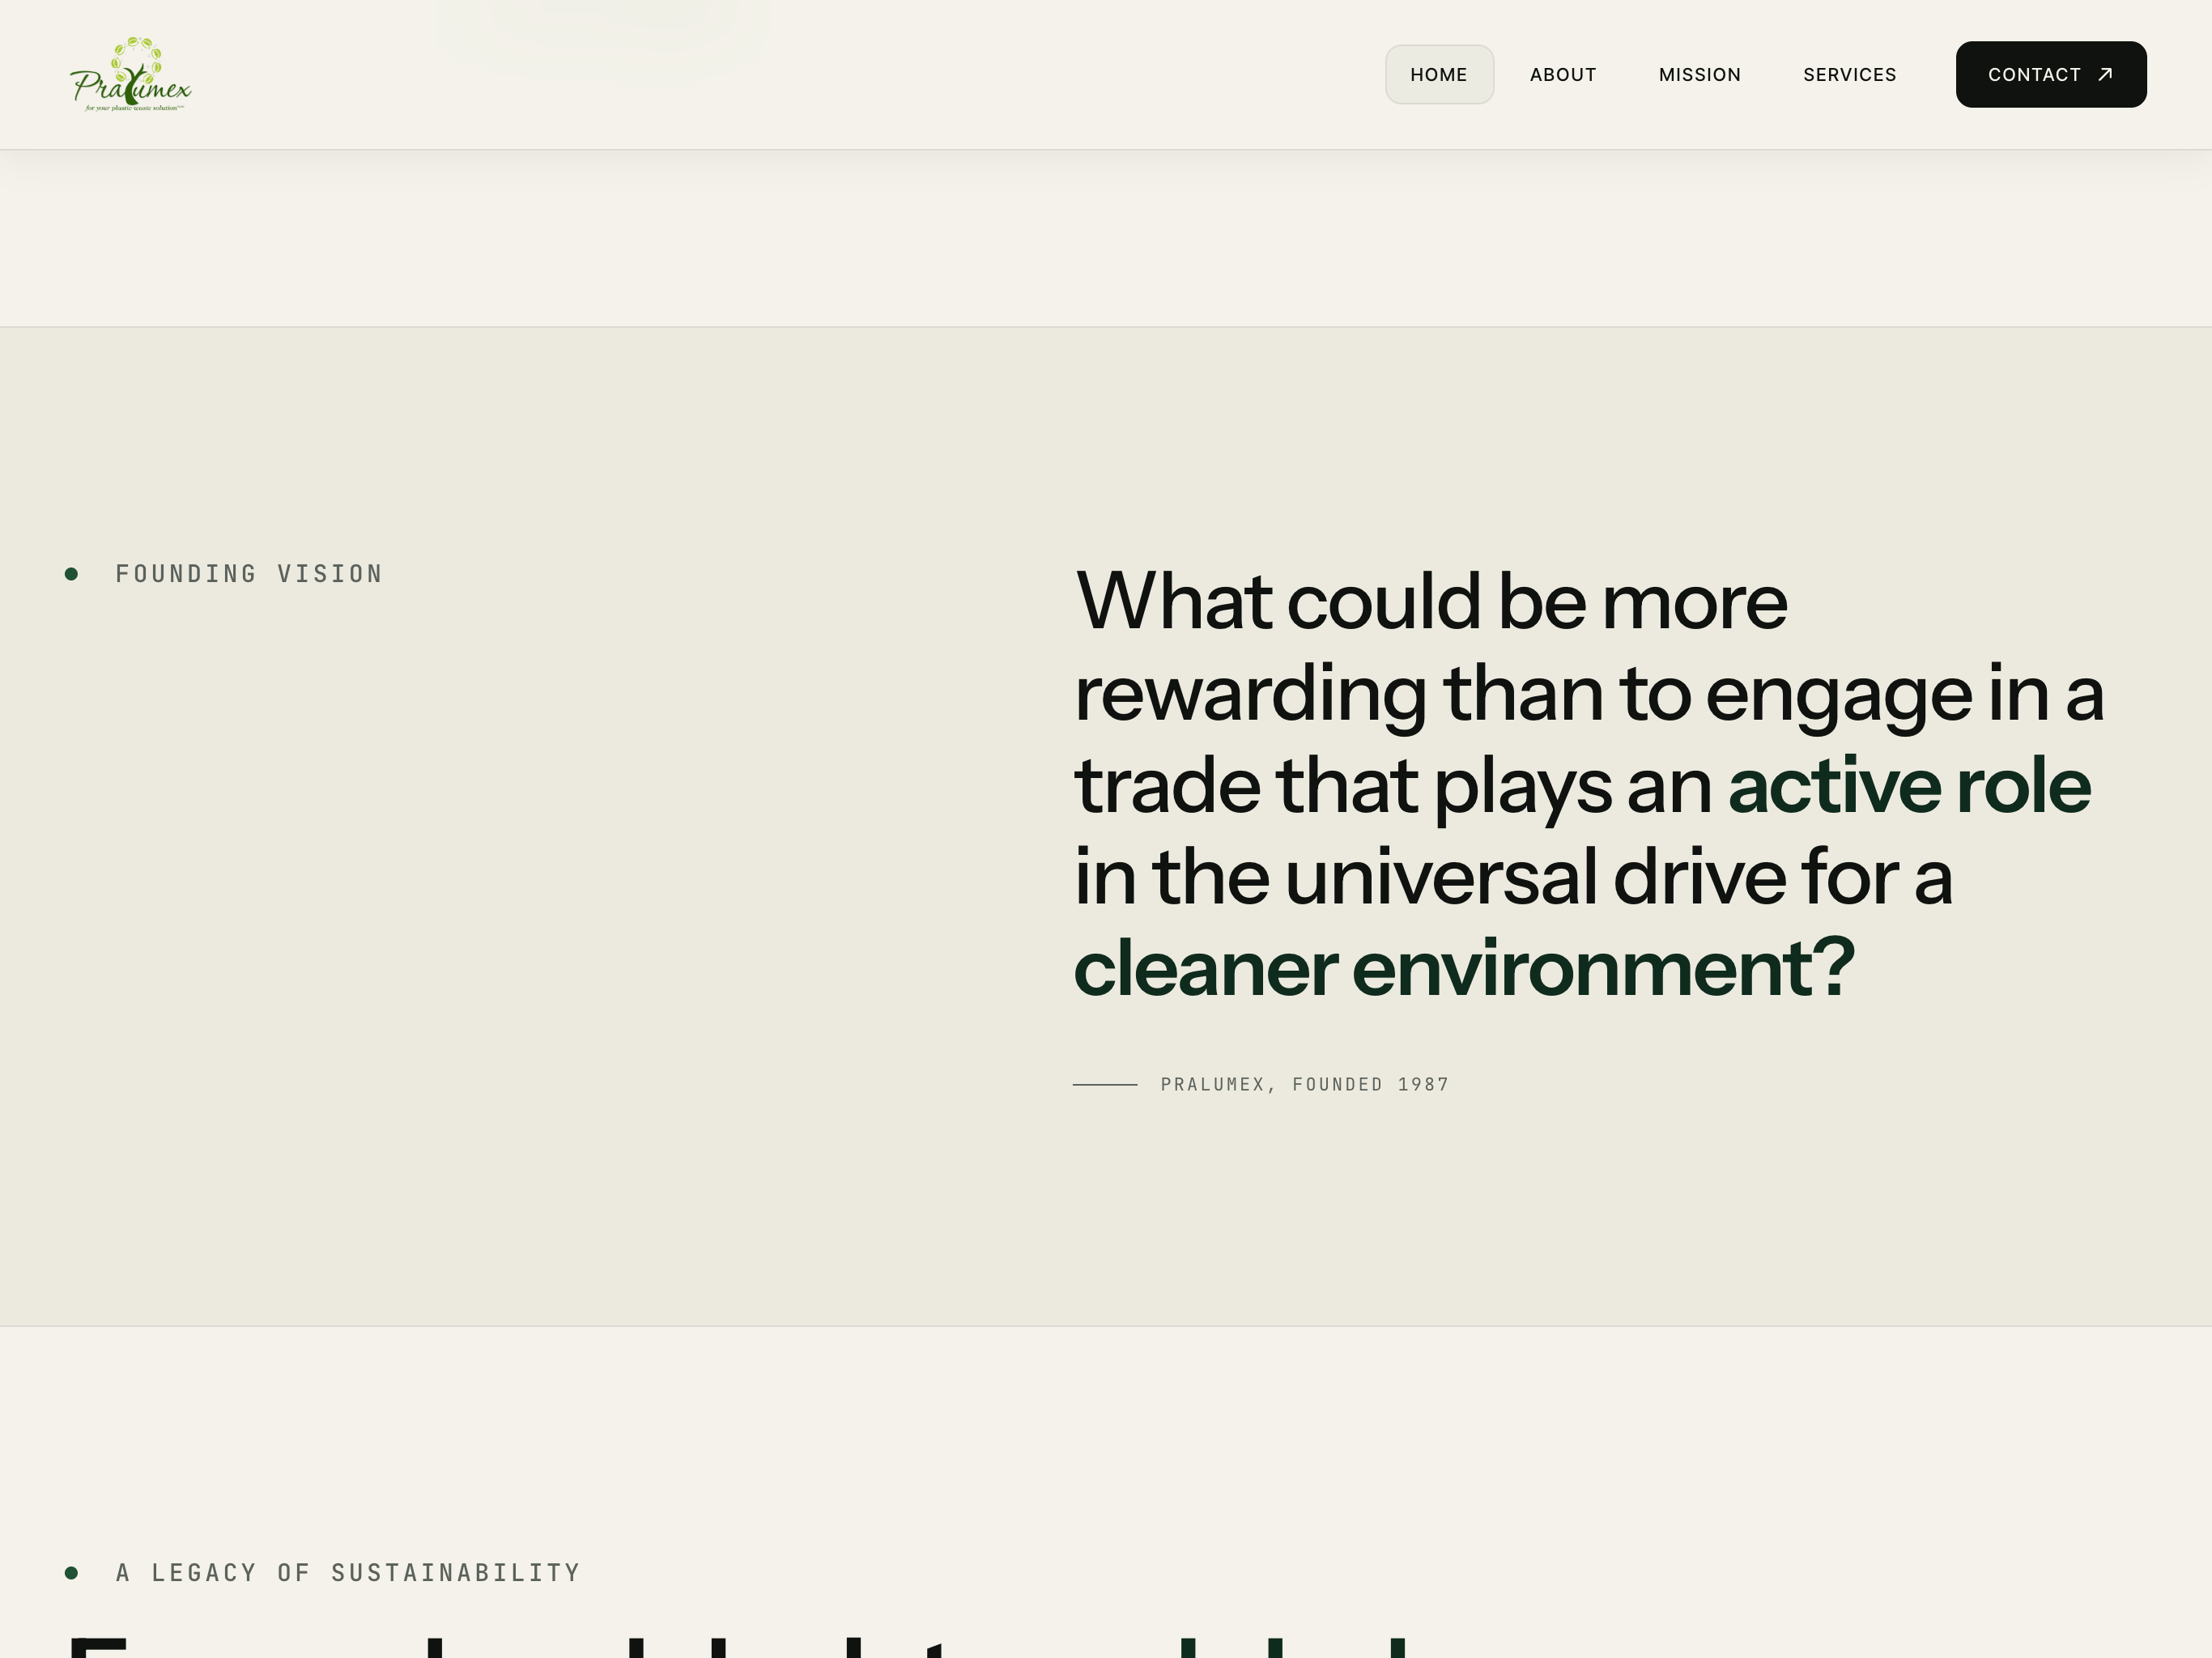
\includegraphics[width=\textwidth,height=0.46\textheight,keepaspectratio]{images/pralumex-website/beta/4.png}
            \end{figure}\clearpage
            \begin{figure}[H]\centering
            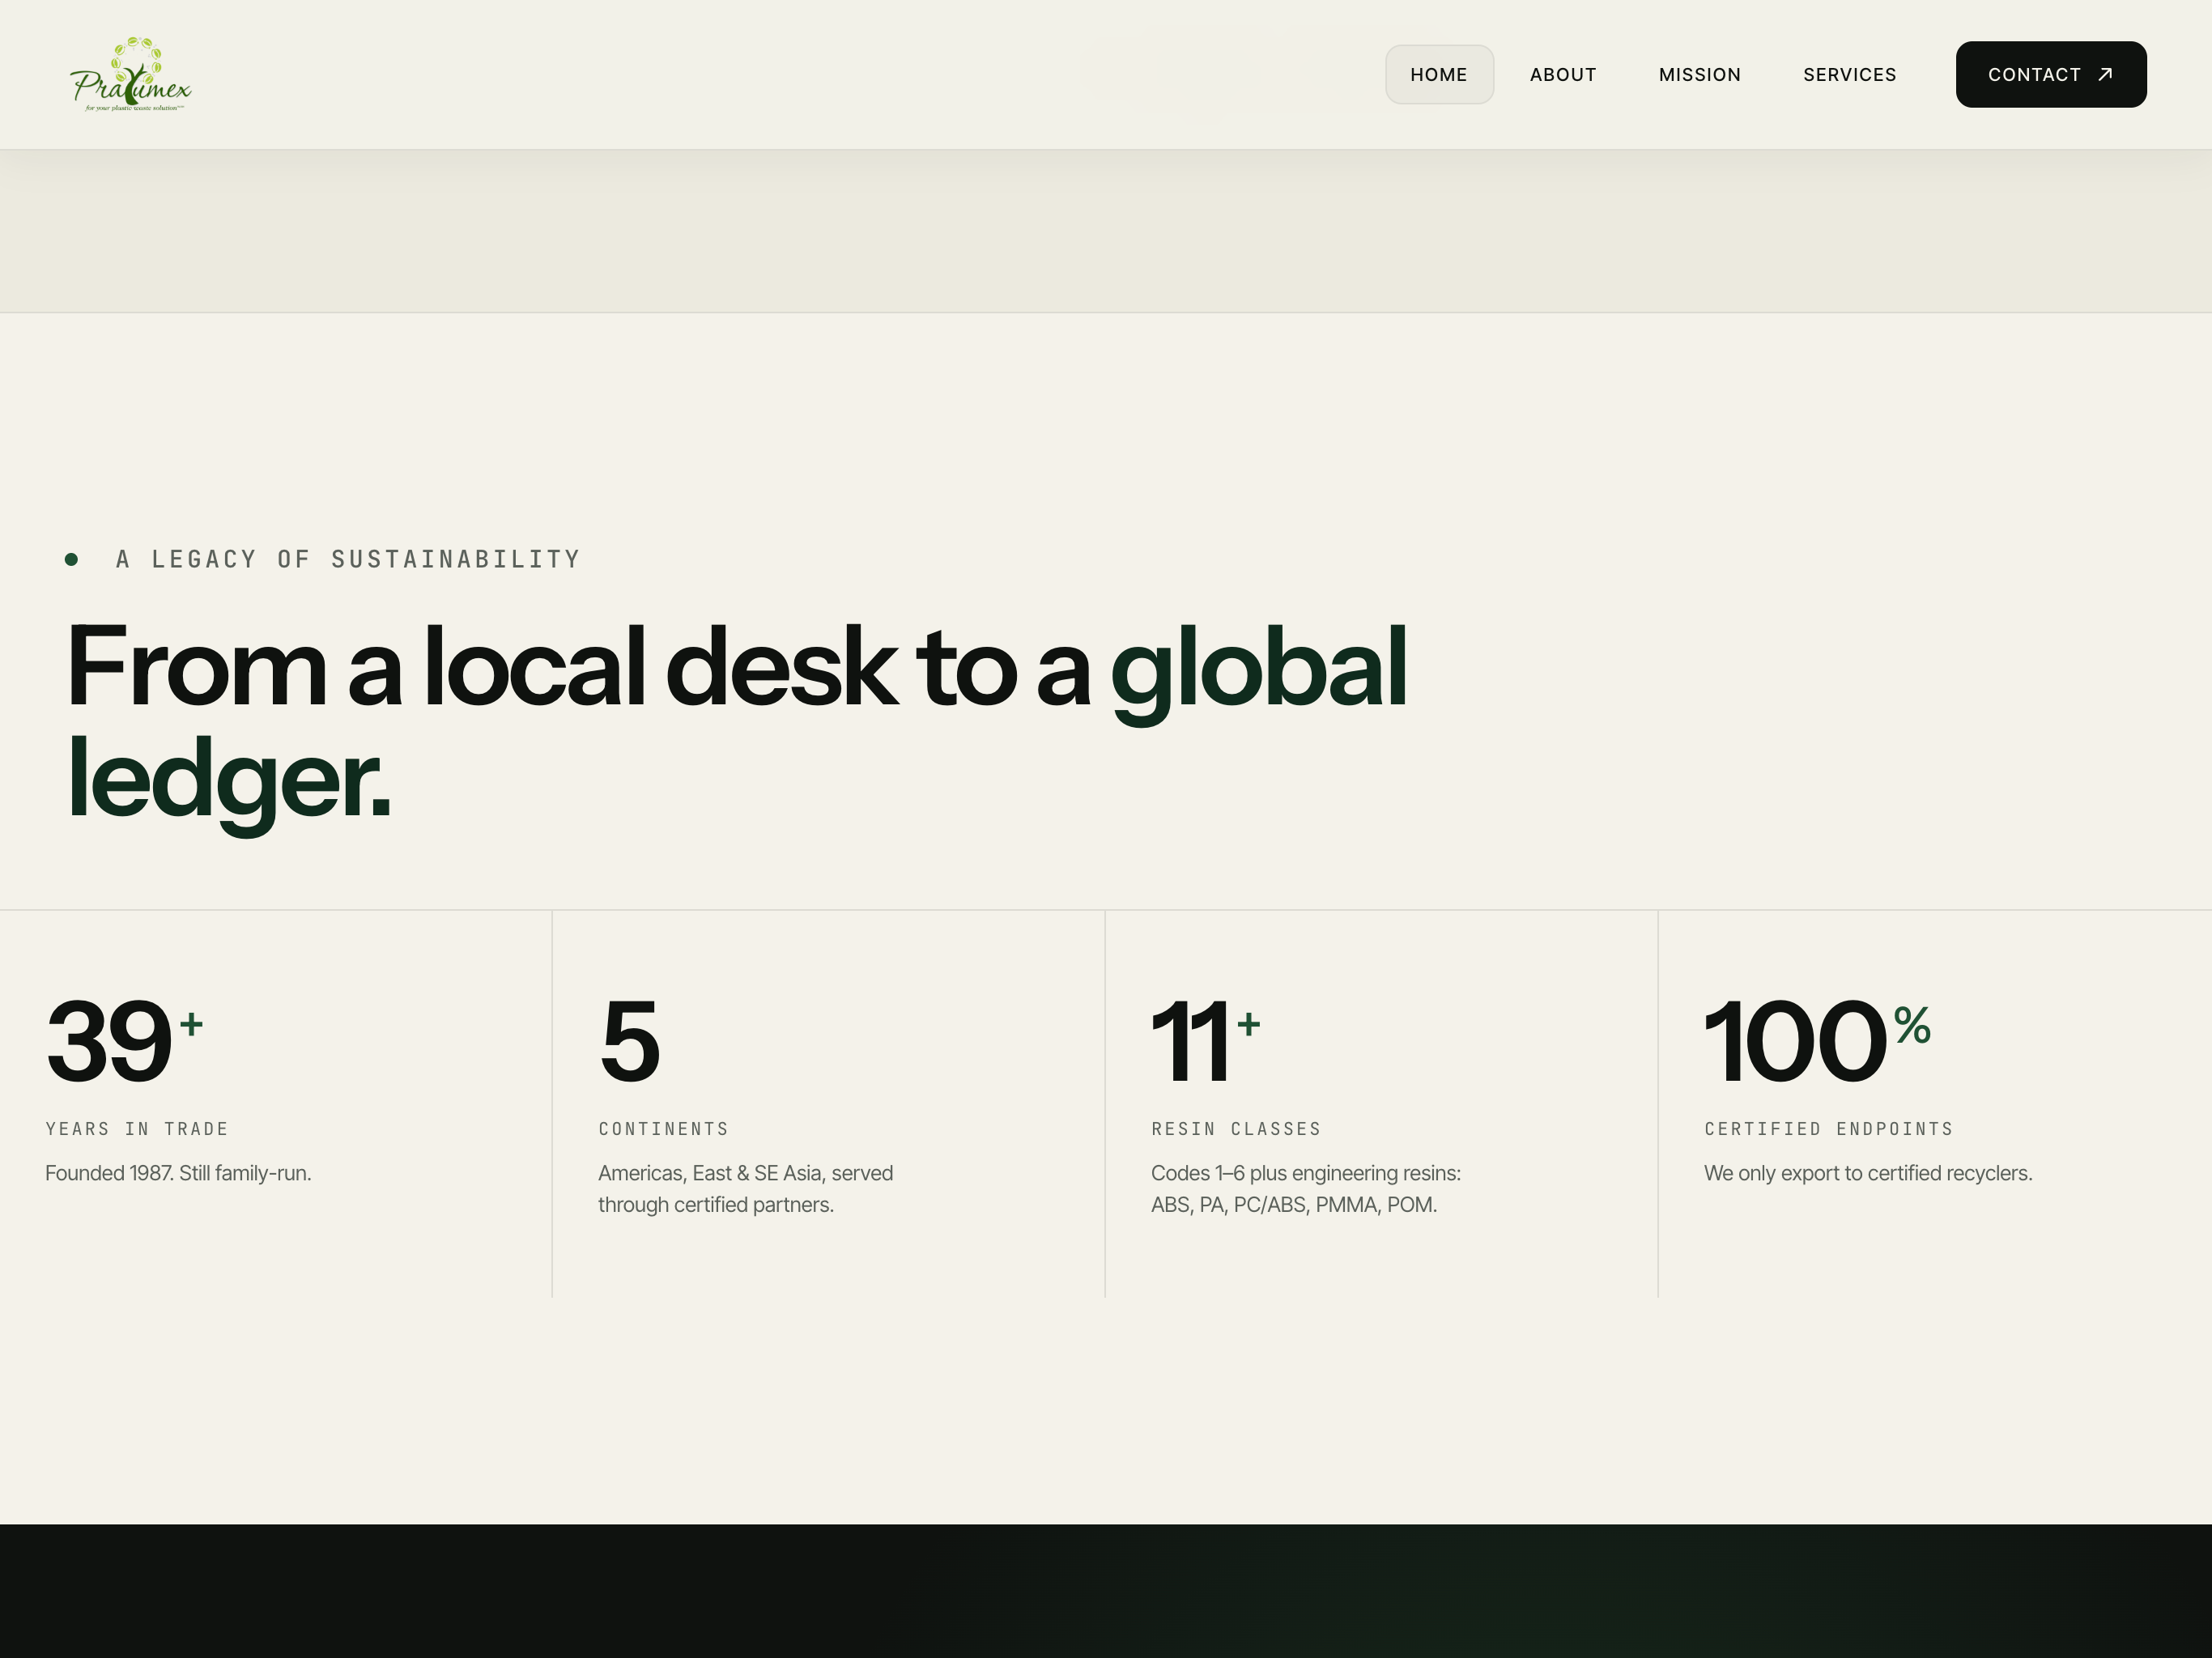
\includegraphics[width=\textwidth,height=0.46\textheight,keepaspectratio]{images/pralumex-website/beta/5.png}\\[4pt]
            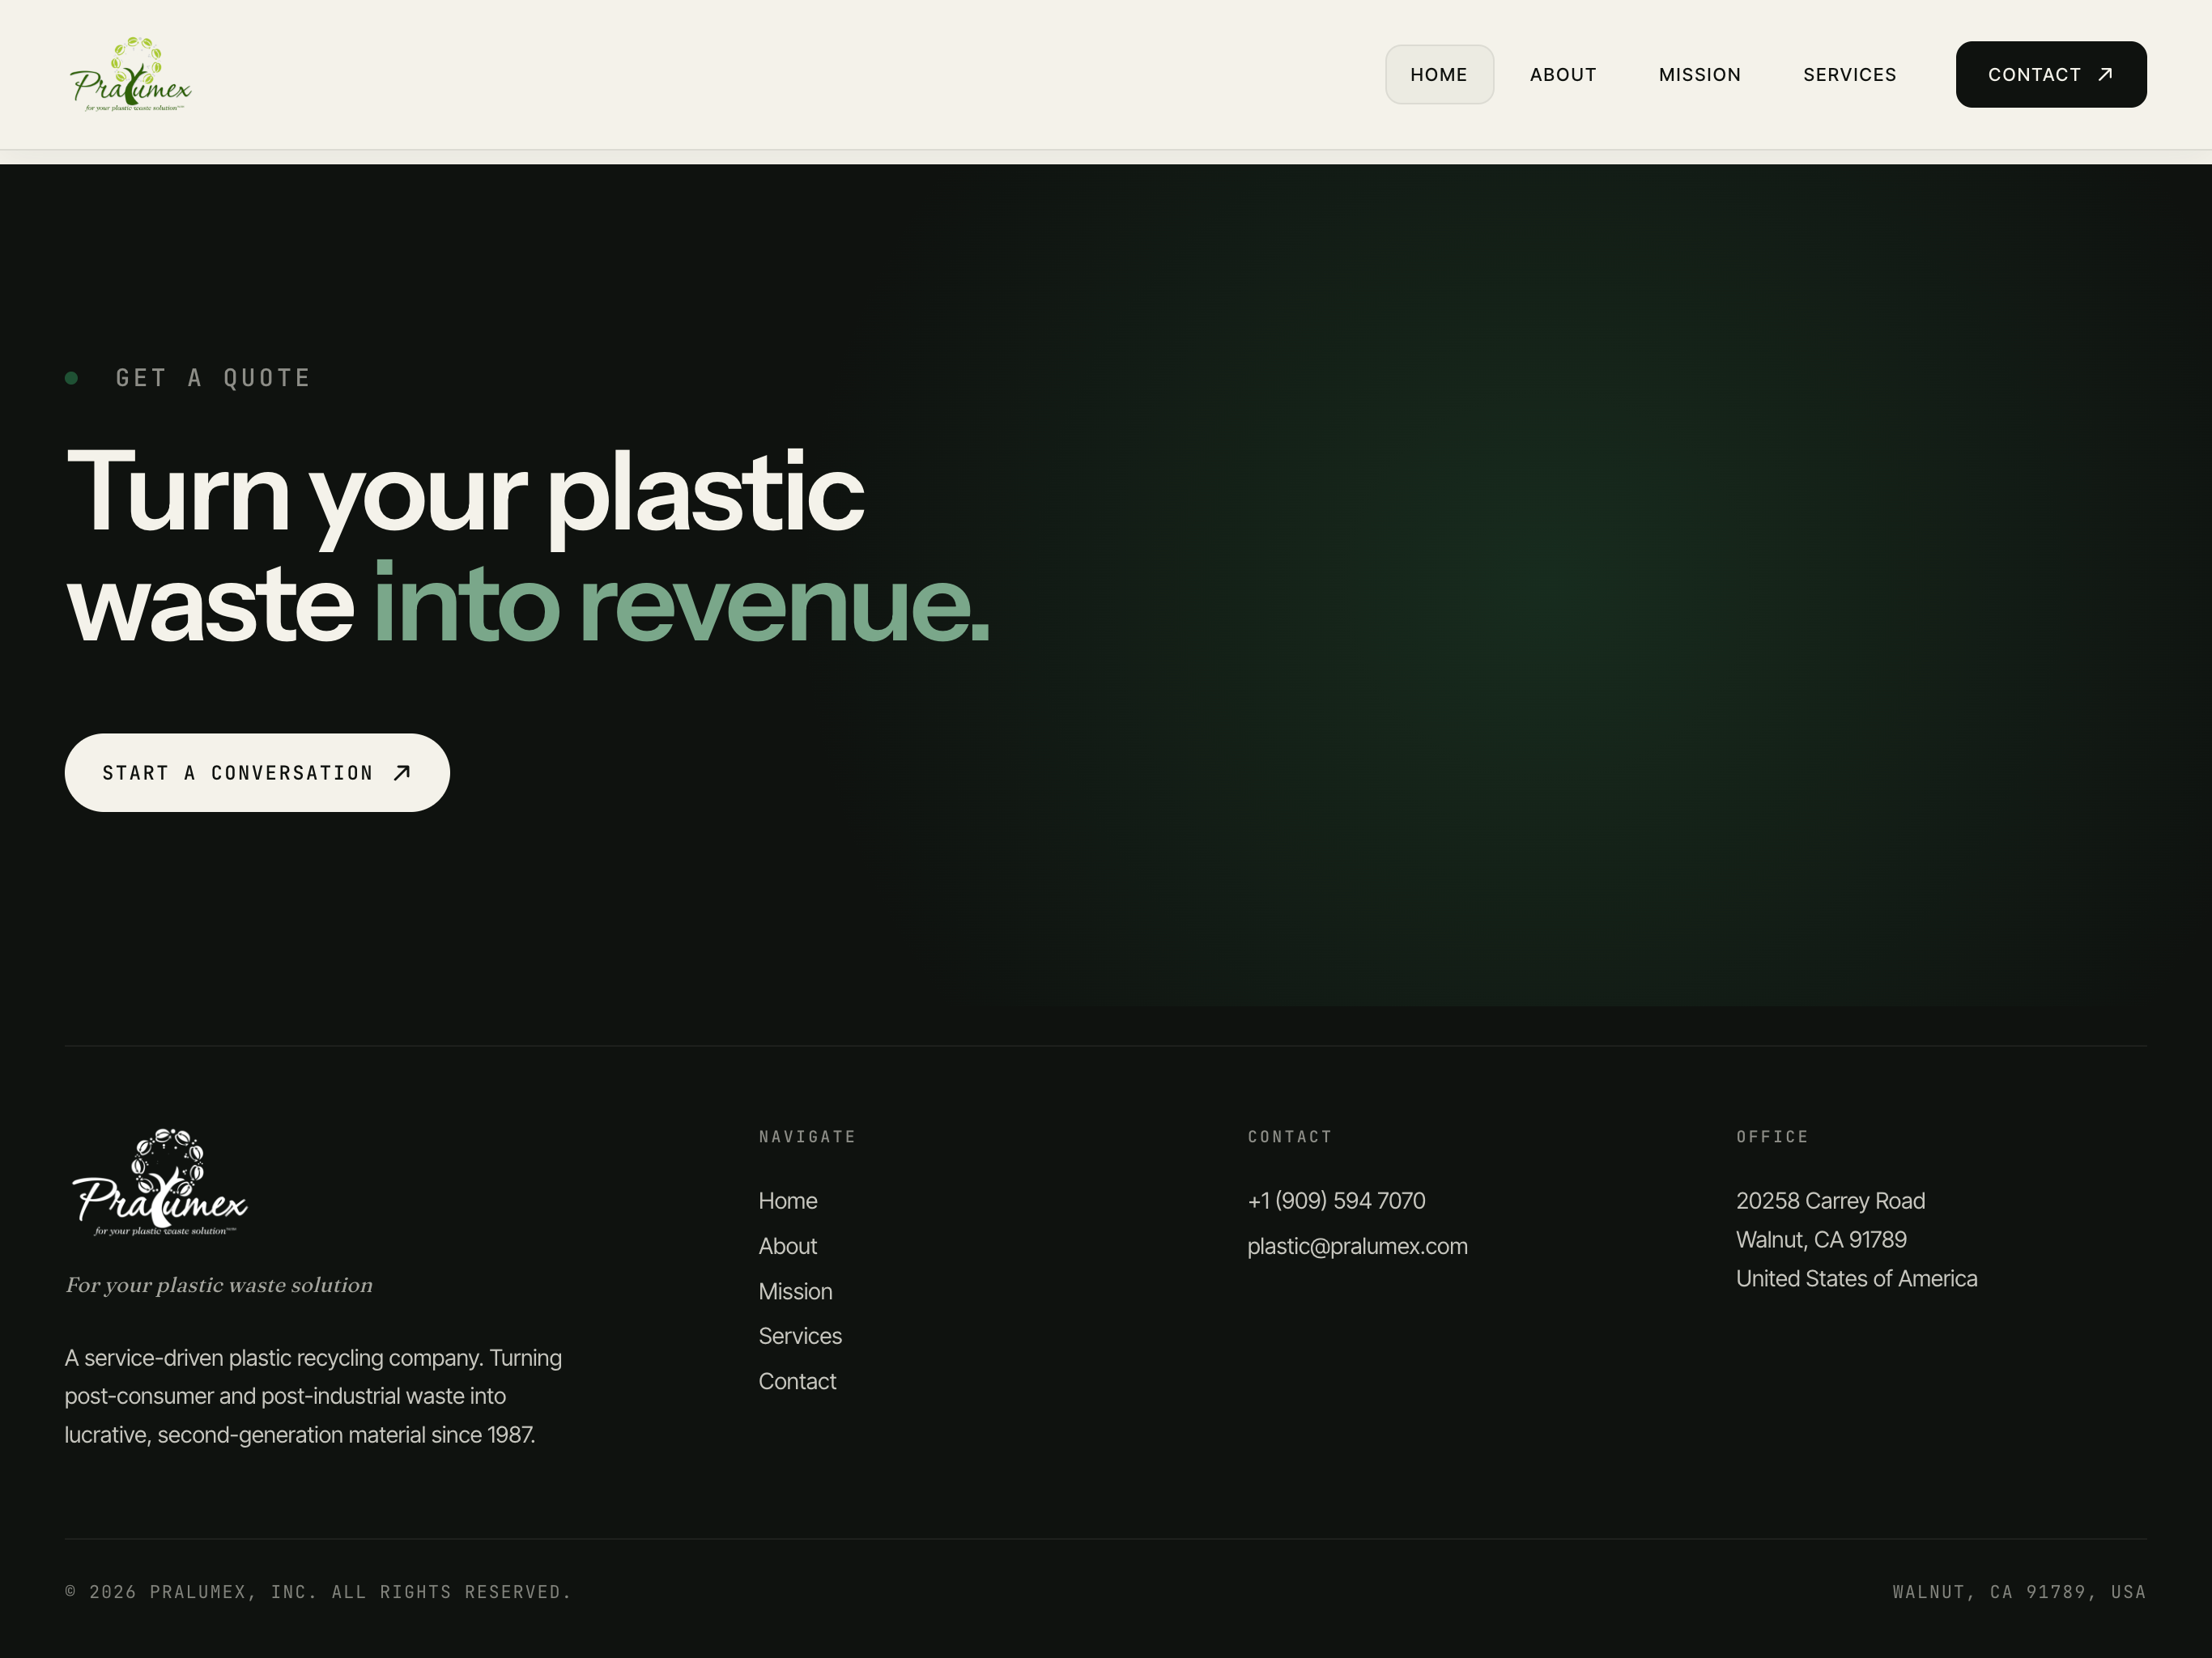
\includegraphics[width=\textwidth,height=0.46\textheight,keepaspectratio]{images/pralumex-website/beta/6.png}
            \end{figure}\clearpage
            \begin{figure}[H]\centering
            
\includegraphics[width=\textwidth,height=0.46\textheight,keepaspectratio]{images/pralumex-website/beta/7.png}\\[4pt]
            
\includegraphics[width=\textwidth,height=0.46\textheight,keepaspectratio]{images/pralumex-website/beta/8.png}
            \end{figure}\clearpage
            \begin{figure}[H]\centering
            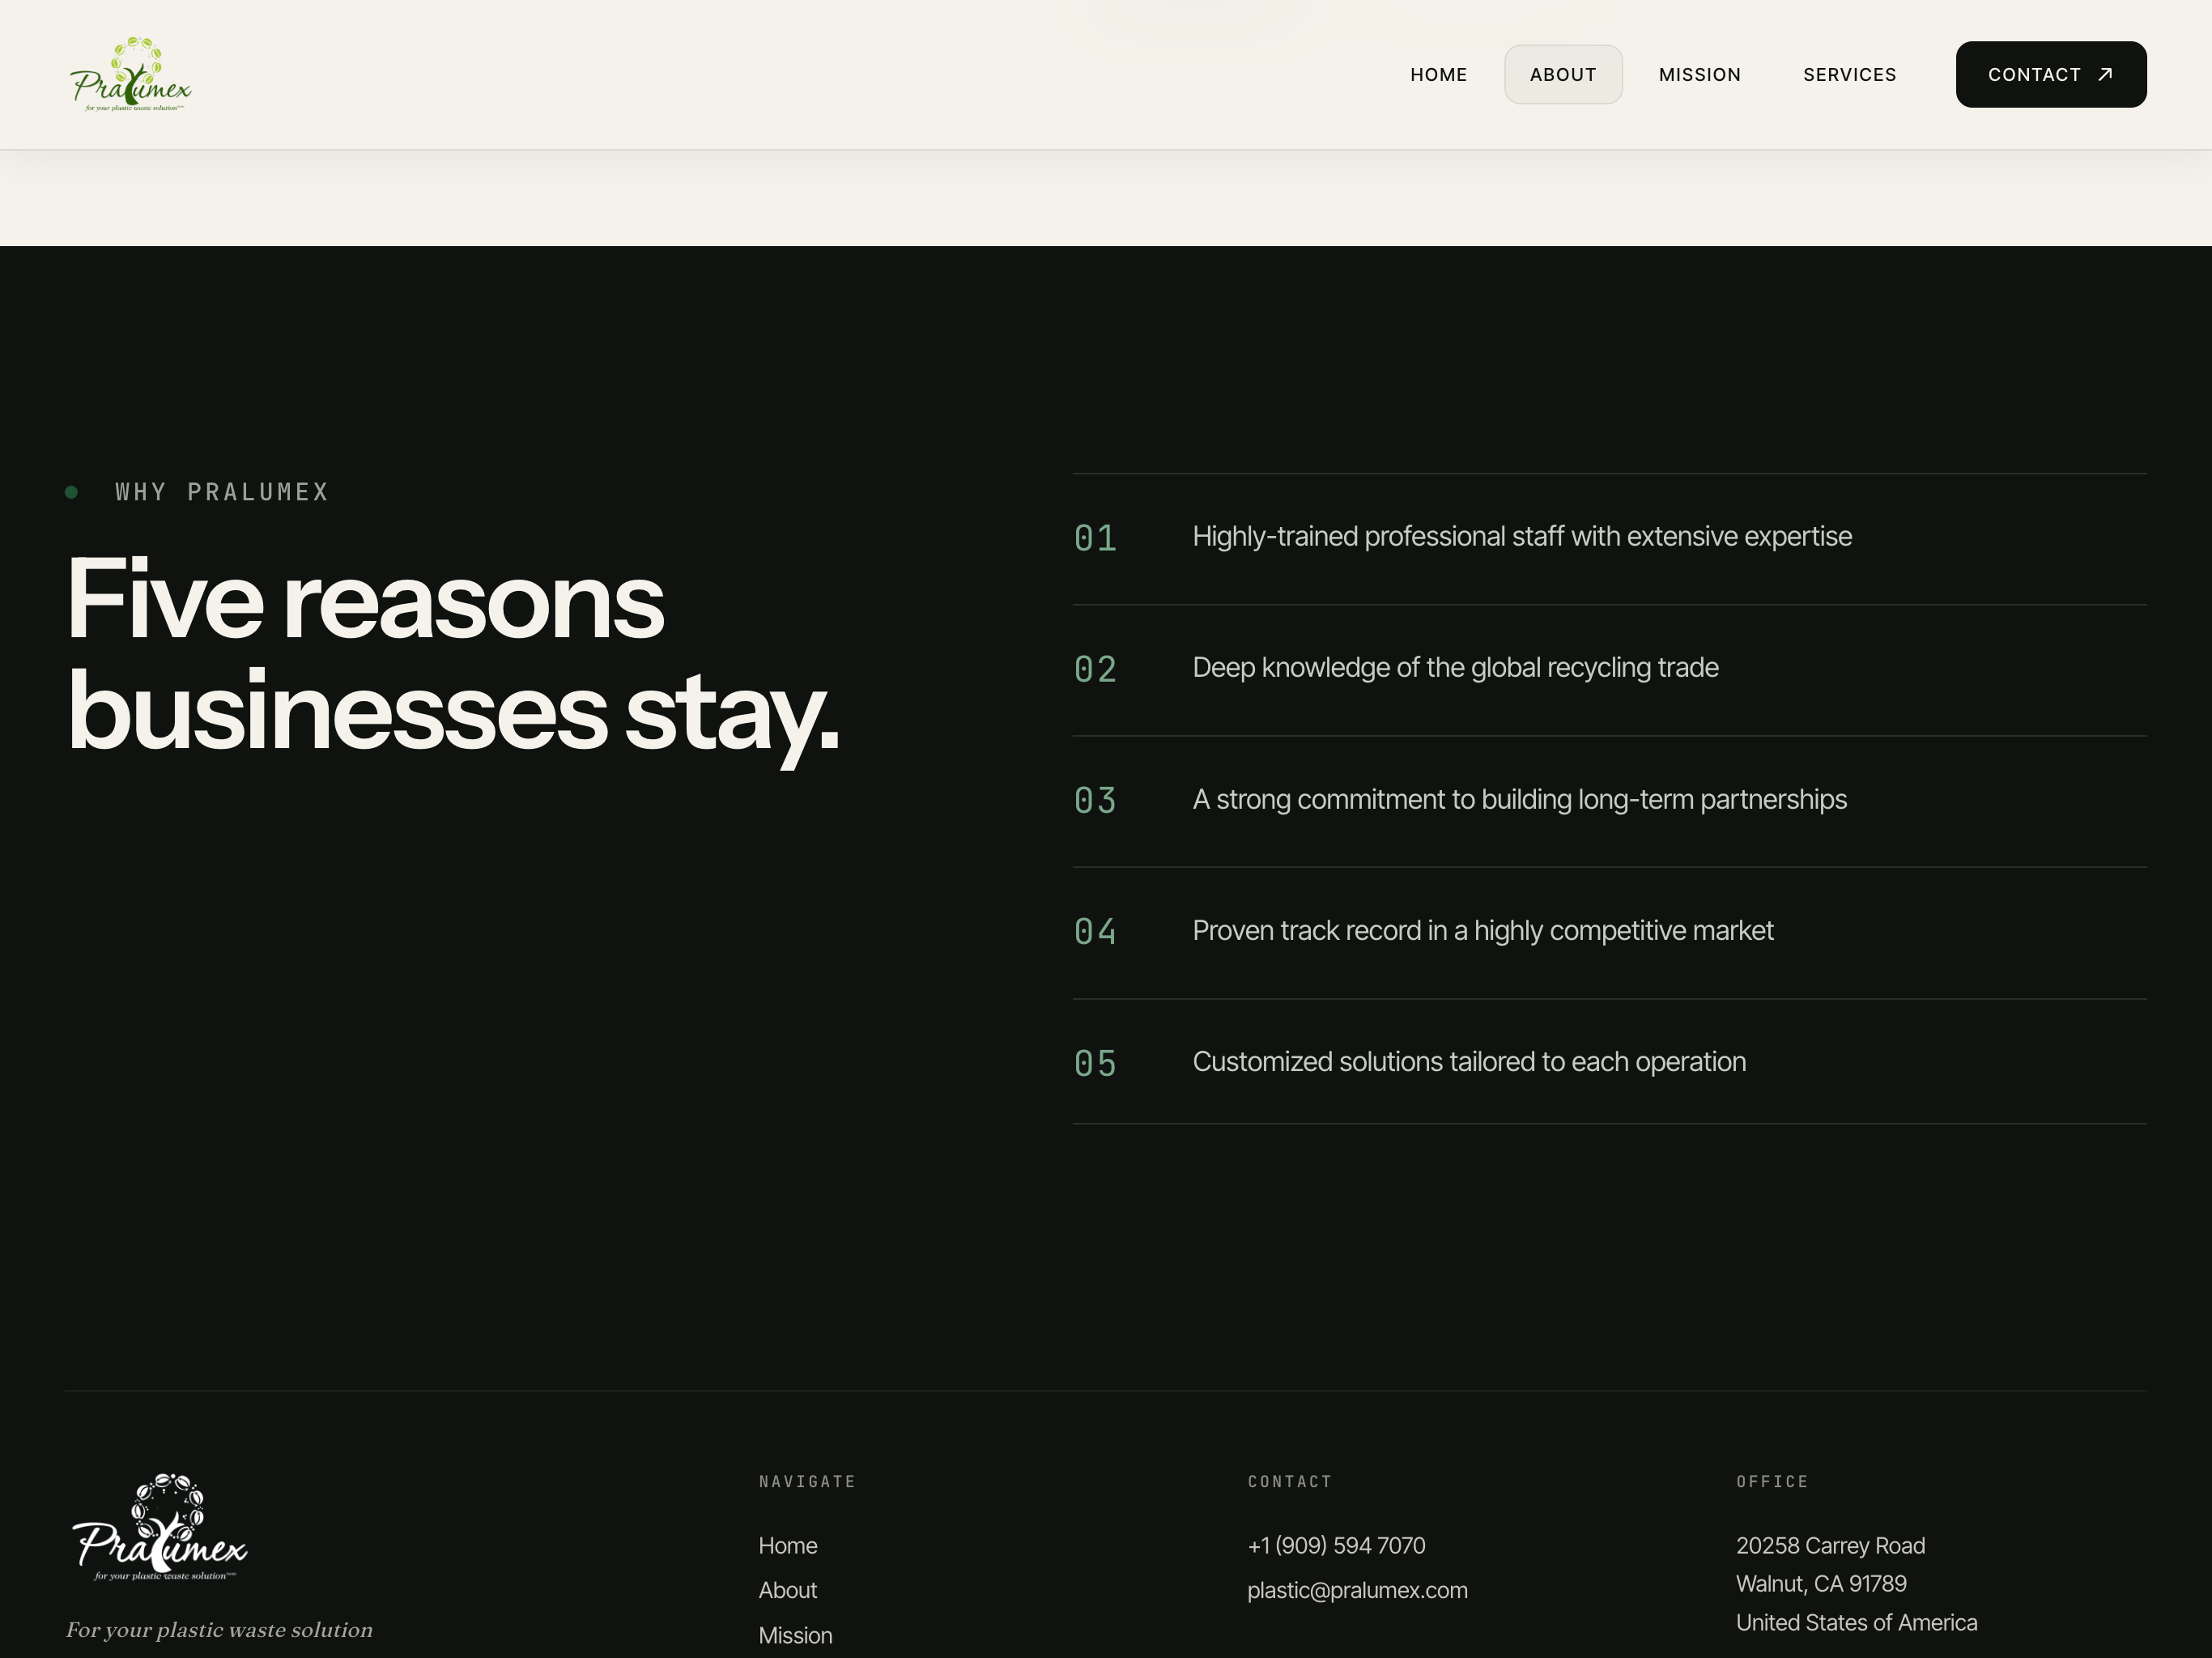
\includegraphics[width=\textwidth,height=0.46\textheight,keepaspectratio]{images/pralumex-website/beta/9.png}\\[4pt]
            
\includegraphics[width=\textwidth,height=0.46\textheight,keepaspectratio]{images/pralumex-website/beta/10.png}
            \end{figure}\clearpage
            \begin{figure}[H]\centering
            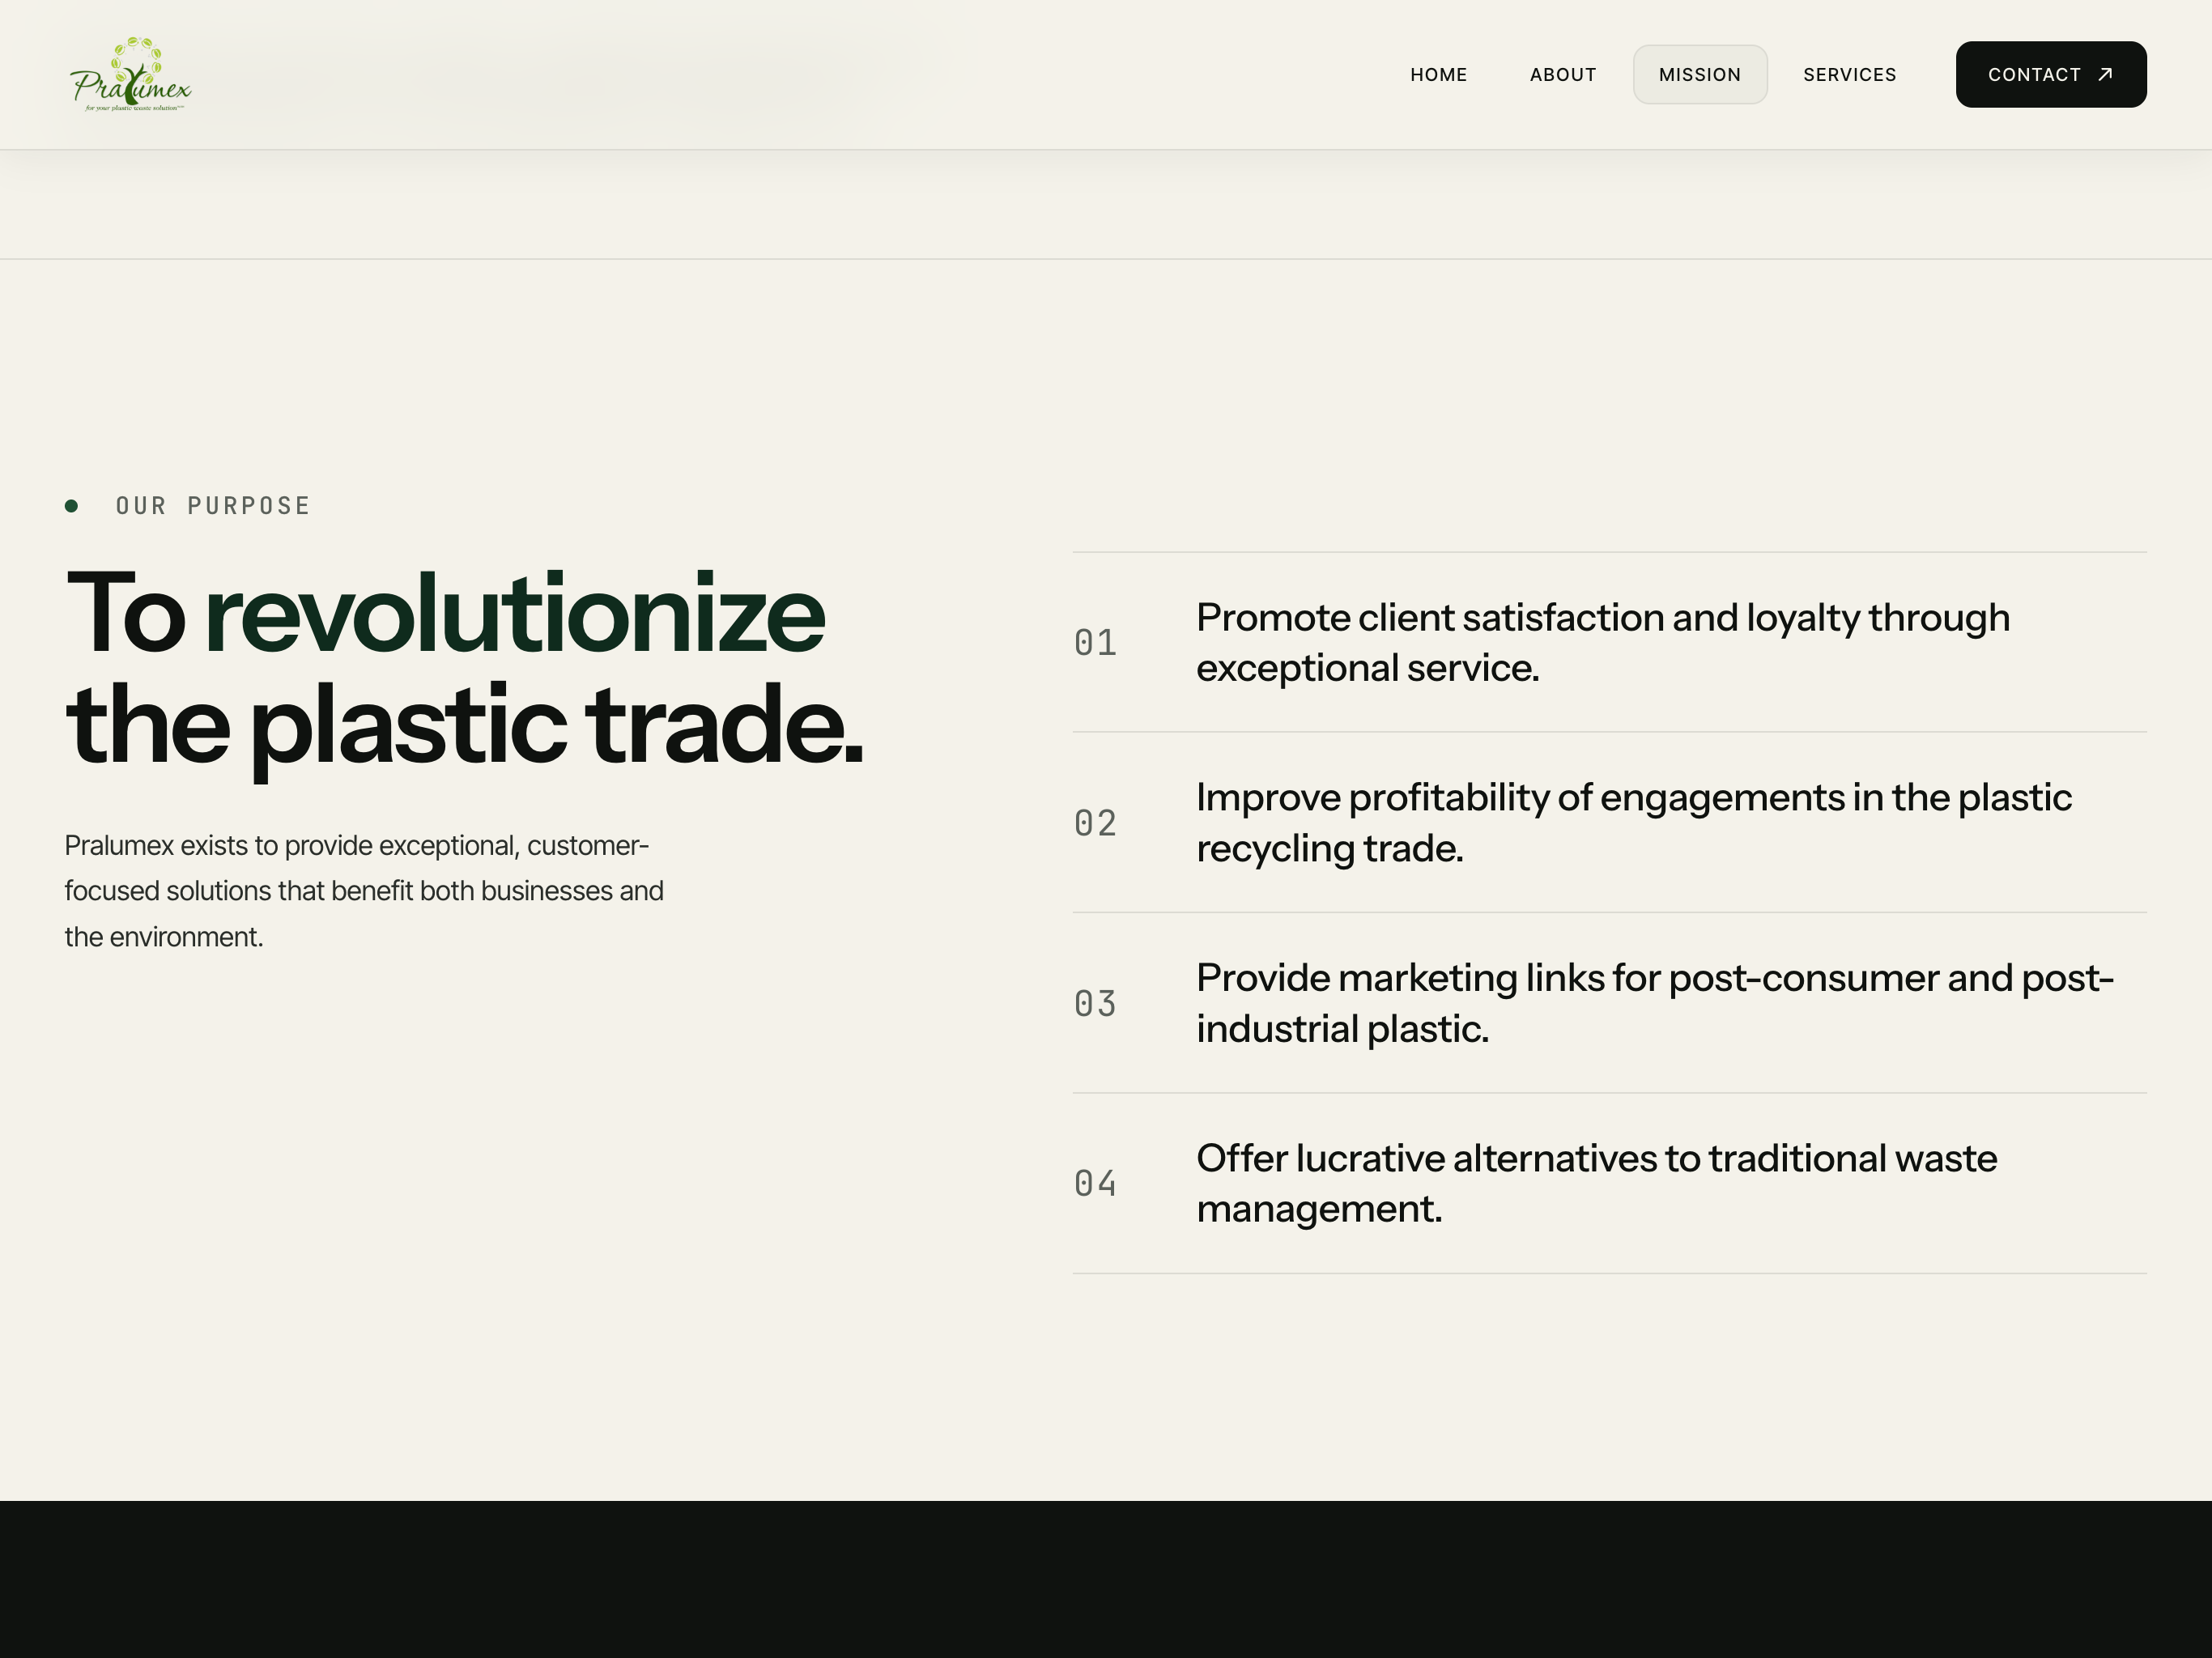
\includegraphics[width=\textwidth,height=0.46\textheight,keepaspectratio]{images/pralumex-website/beta/11.png}\\[4pt]
            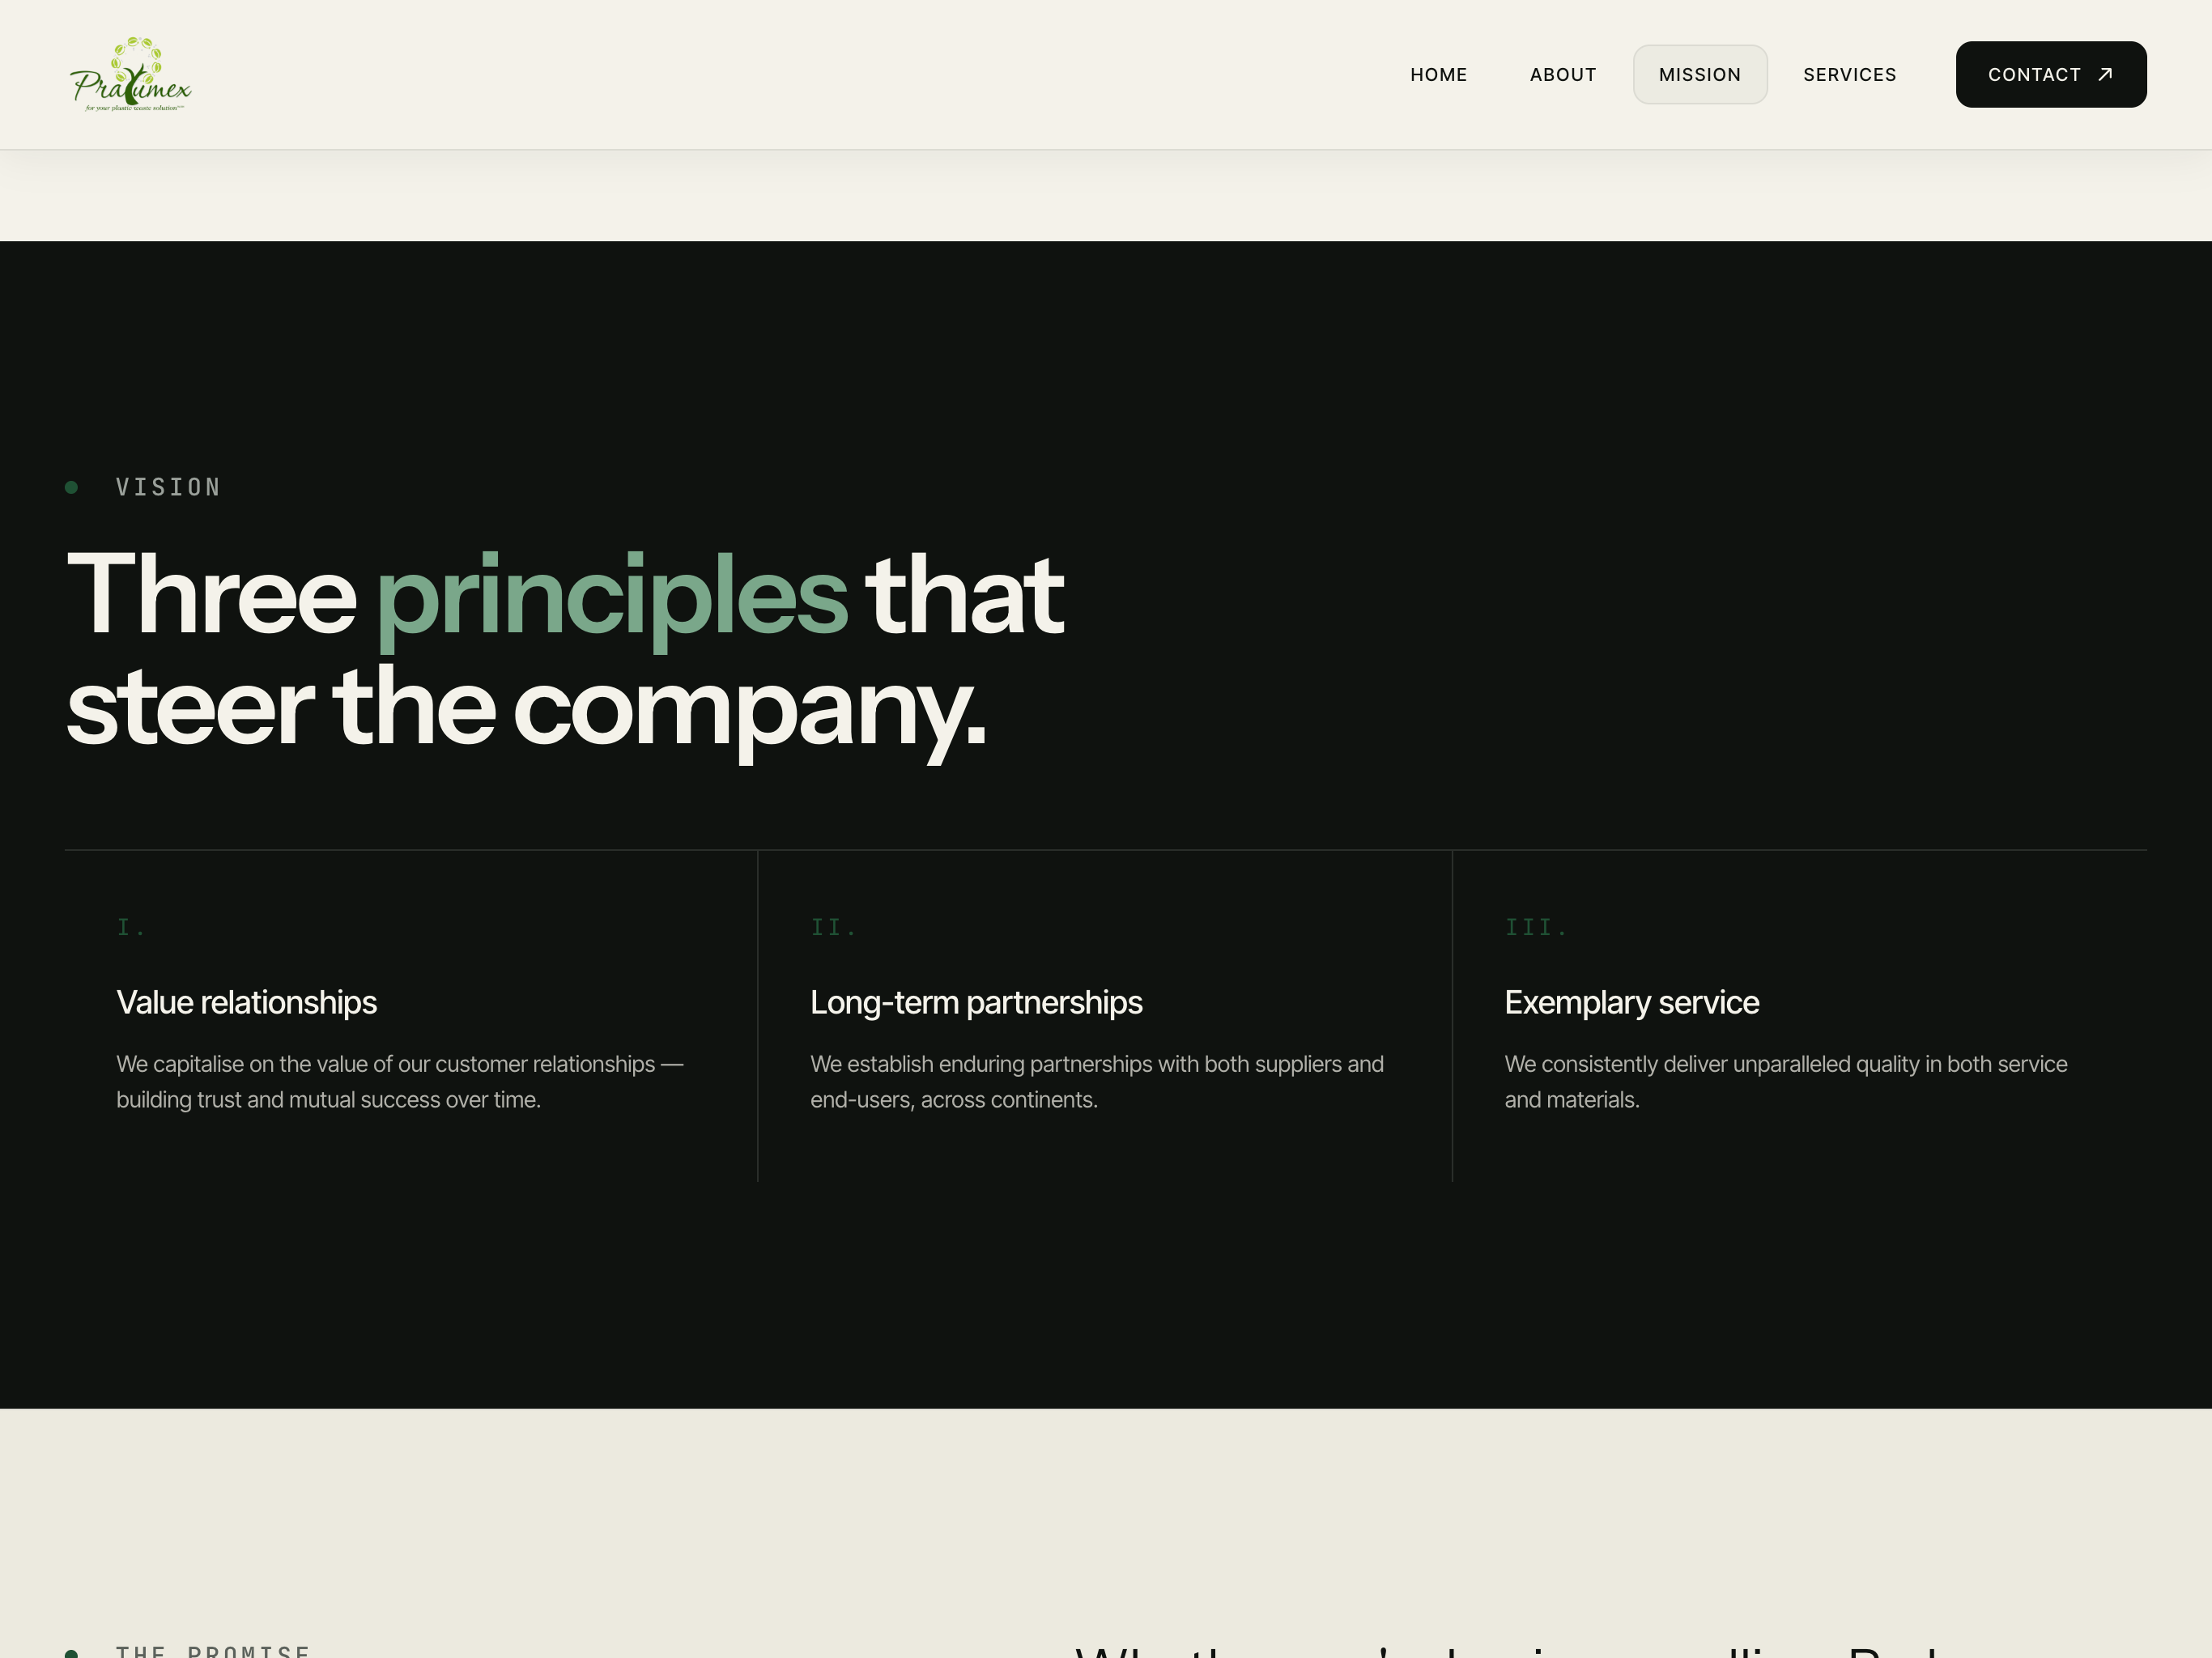
\includegraphics[width=\textwidth,height=0.46\textheight,keepaspectratio]{images/pralumex-website/beta/12.png}
            \end{figure}\clearpage
            \begin{figure}[H]\centering
            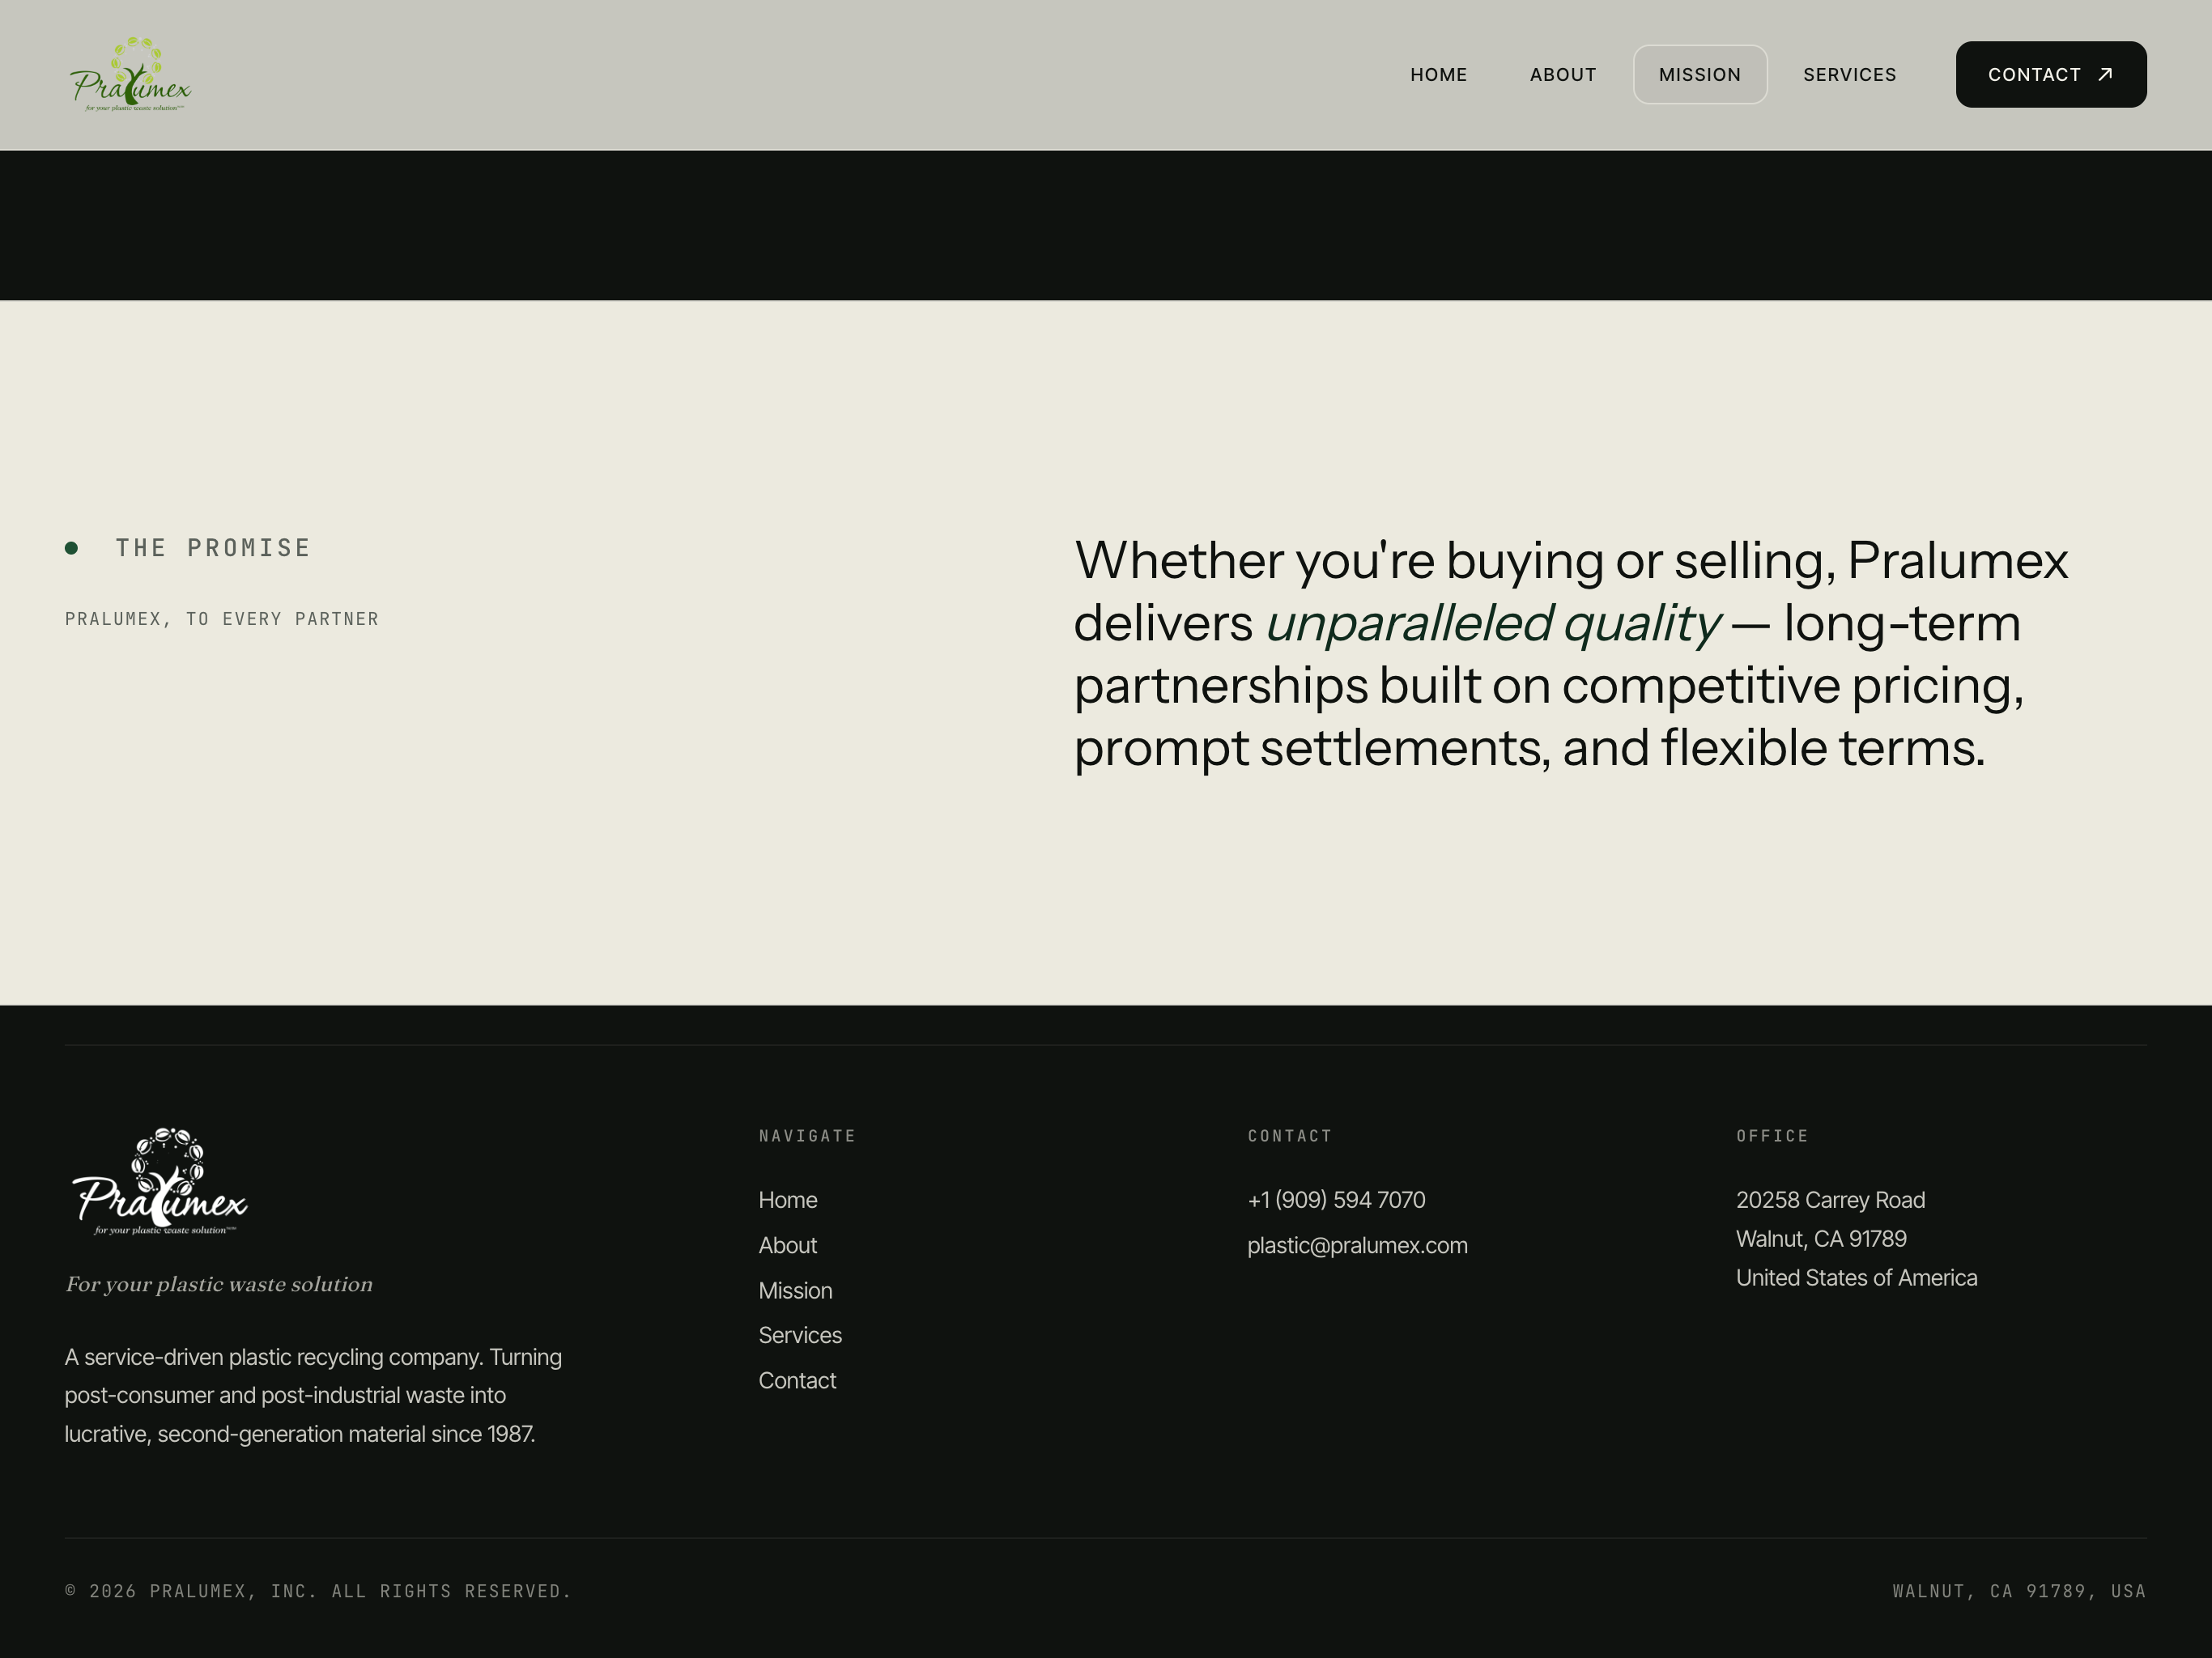
\includegraphics[width=\textwidth,height=0.46\textheight,keepaspectratio]{images/pralumex-website/beta/13.png}\\[4pt]
            
\includegraphics[width=\textwidth,height=0.46\textheight,keepaspectratio]{images/pralumex-website/beta/14.png}
            \end{figure}\clearpage
            \begin{figure}[H]\centering
            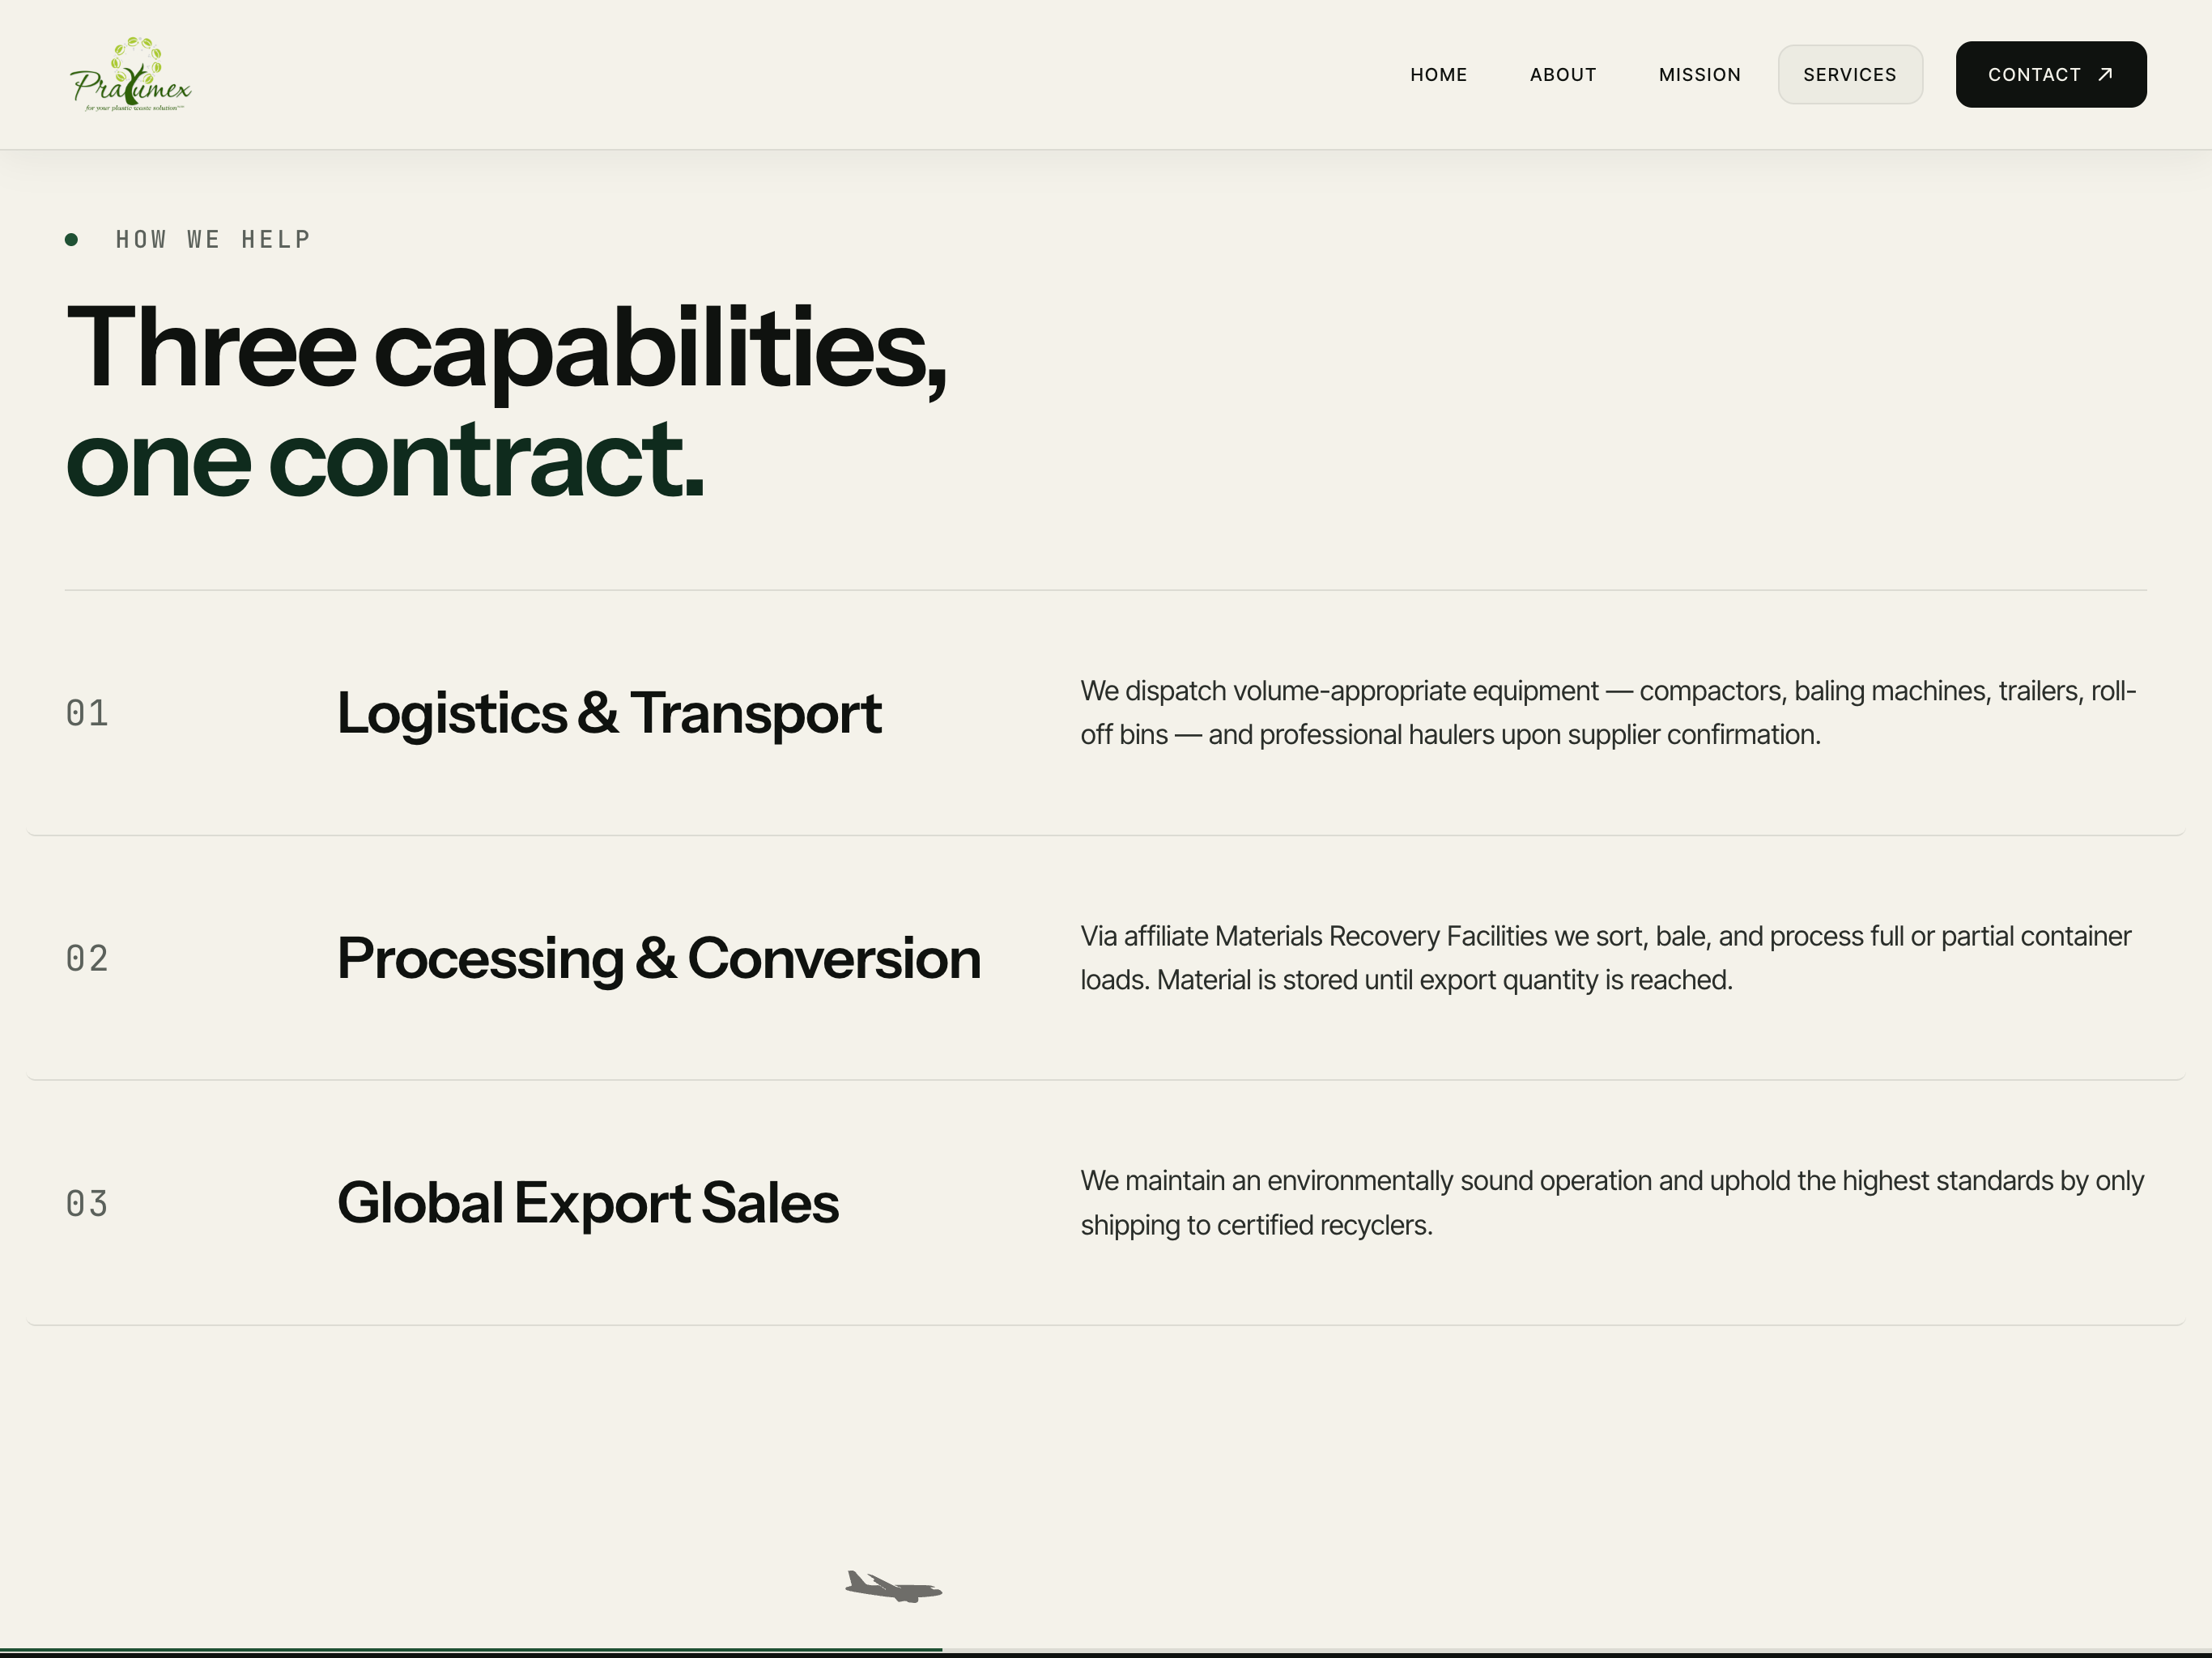
\includegraphics[width=\textwidth,height=0.46\textheight,keepaspectratio]{images/pralumex-website/beta/15.png}\\[4pt]
            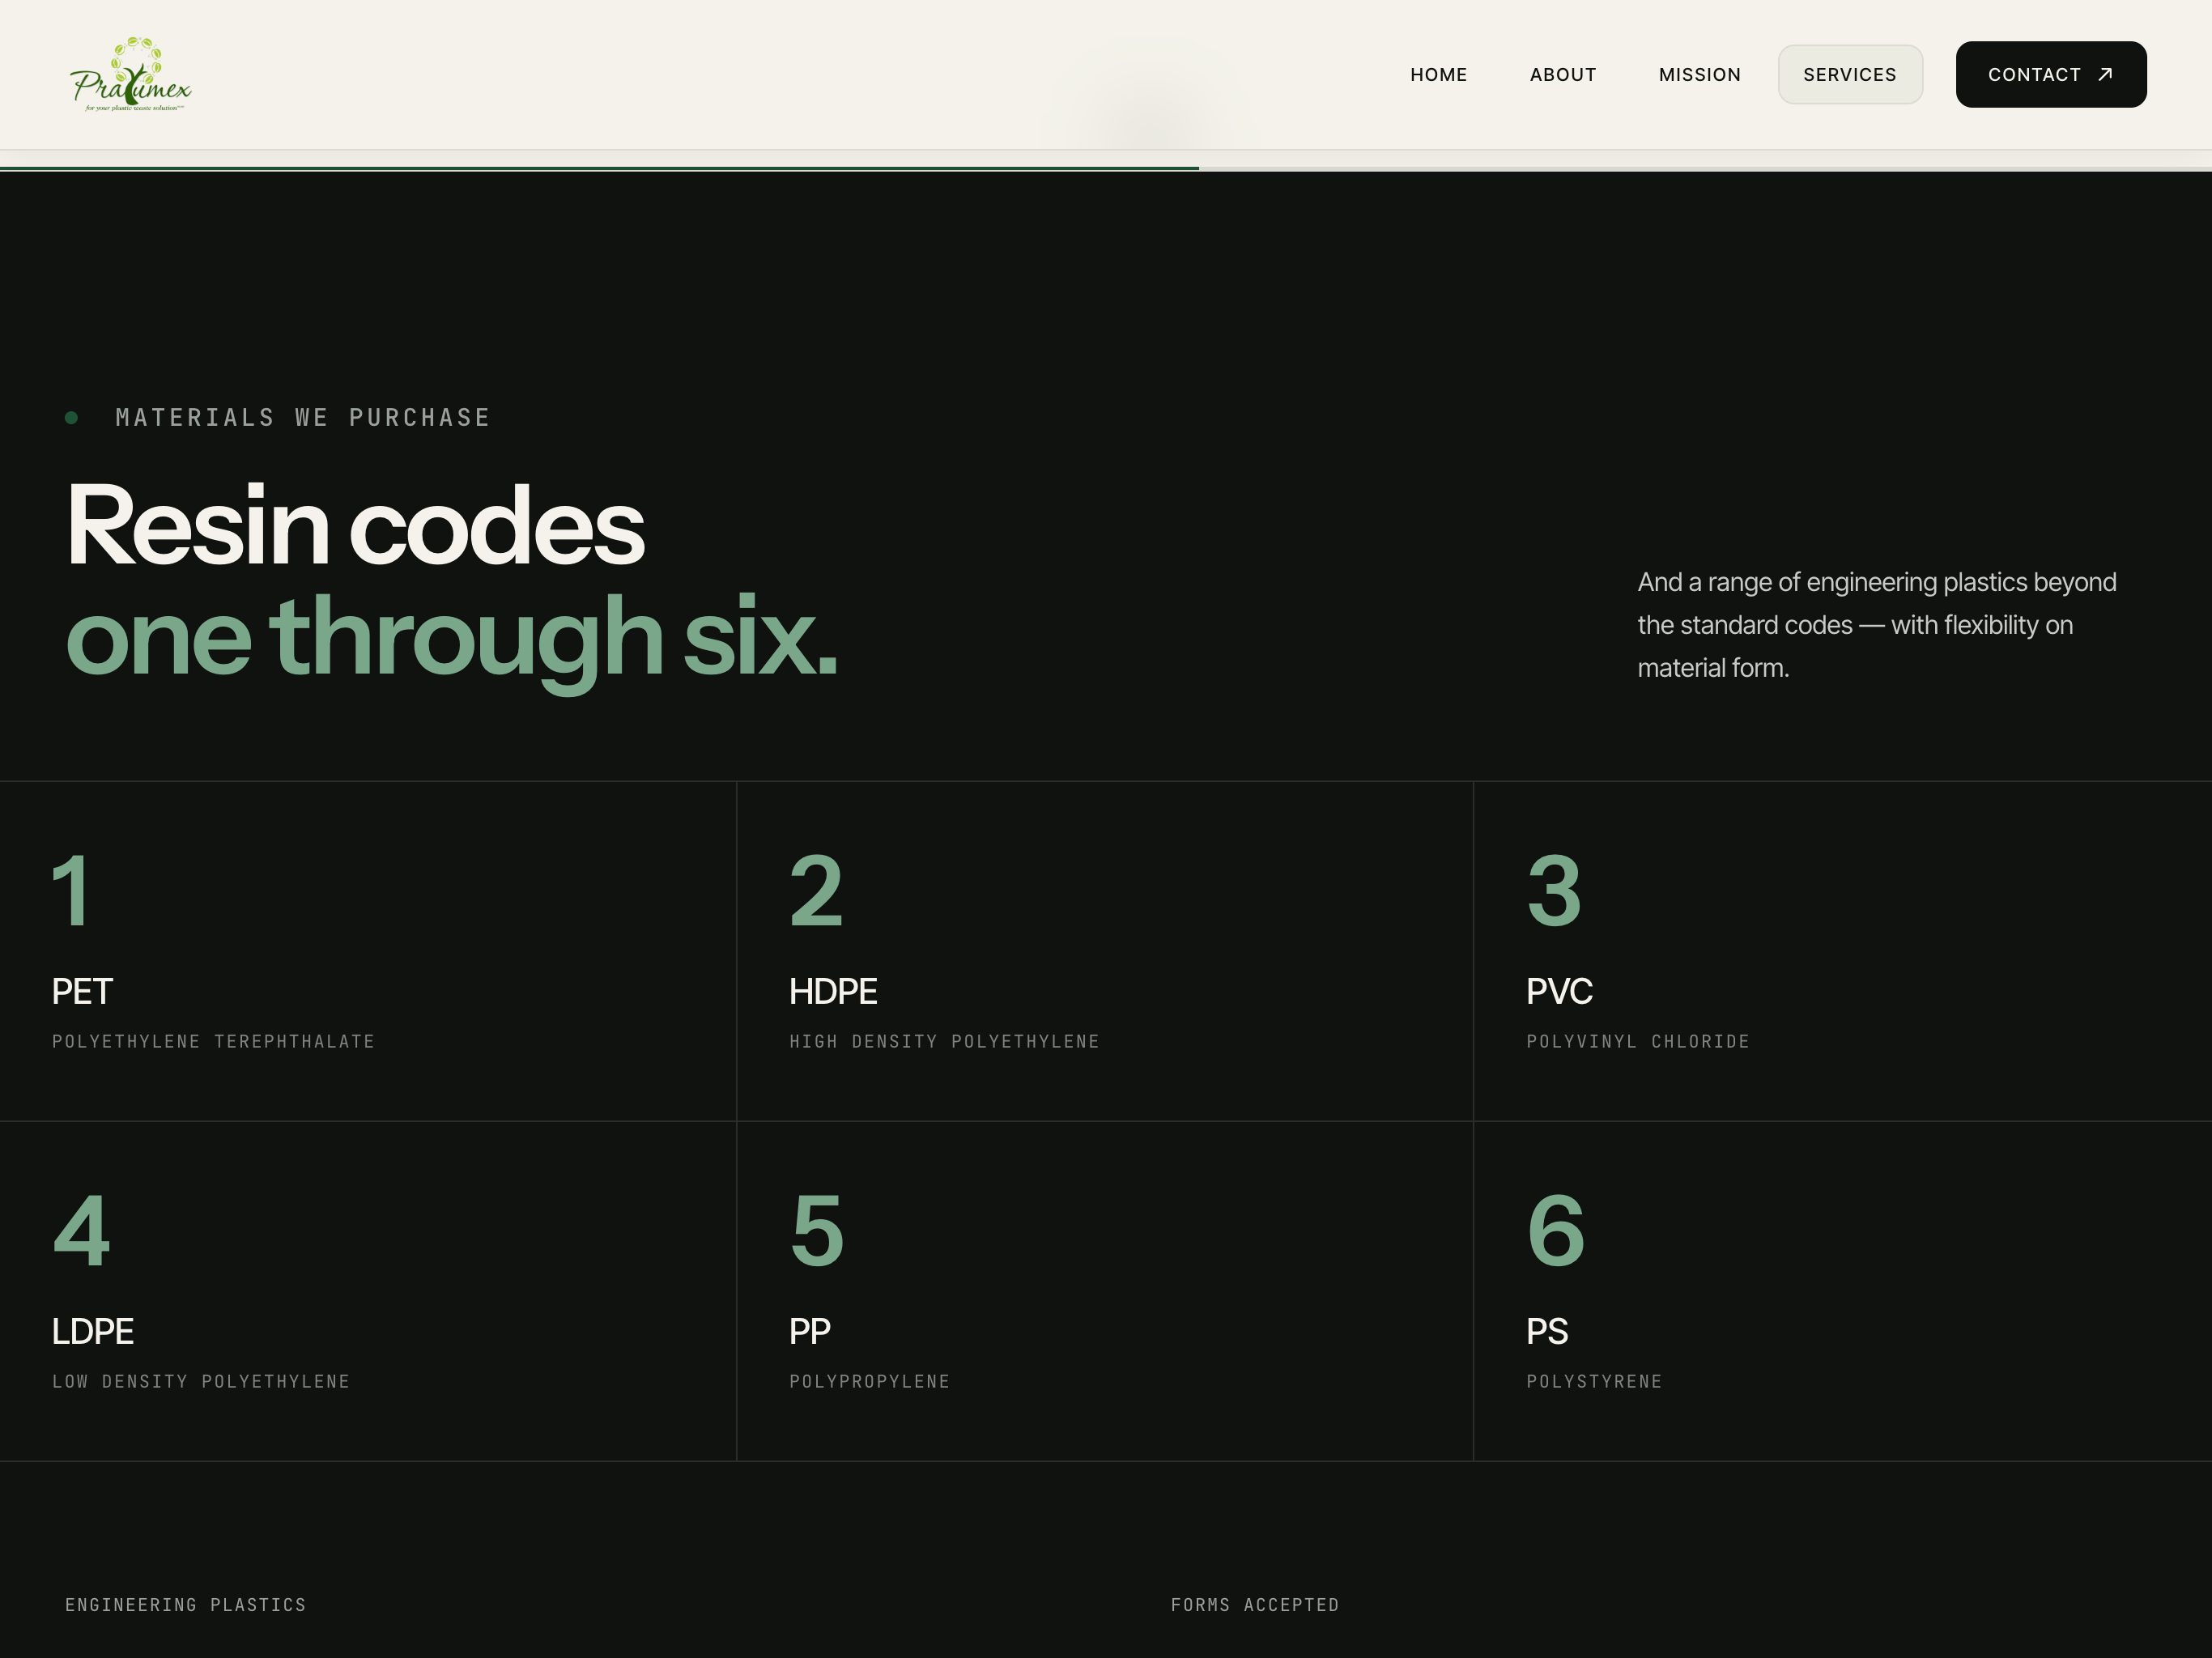
\includegraphics[width=\textwidth,height=0.46\textheight,keepaspectratio]{images/pralumex-website/beta/16.png}
            \end{figure}\clearpage
            \begin{figure}[H]\centering
            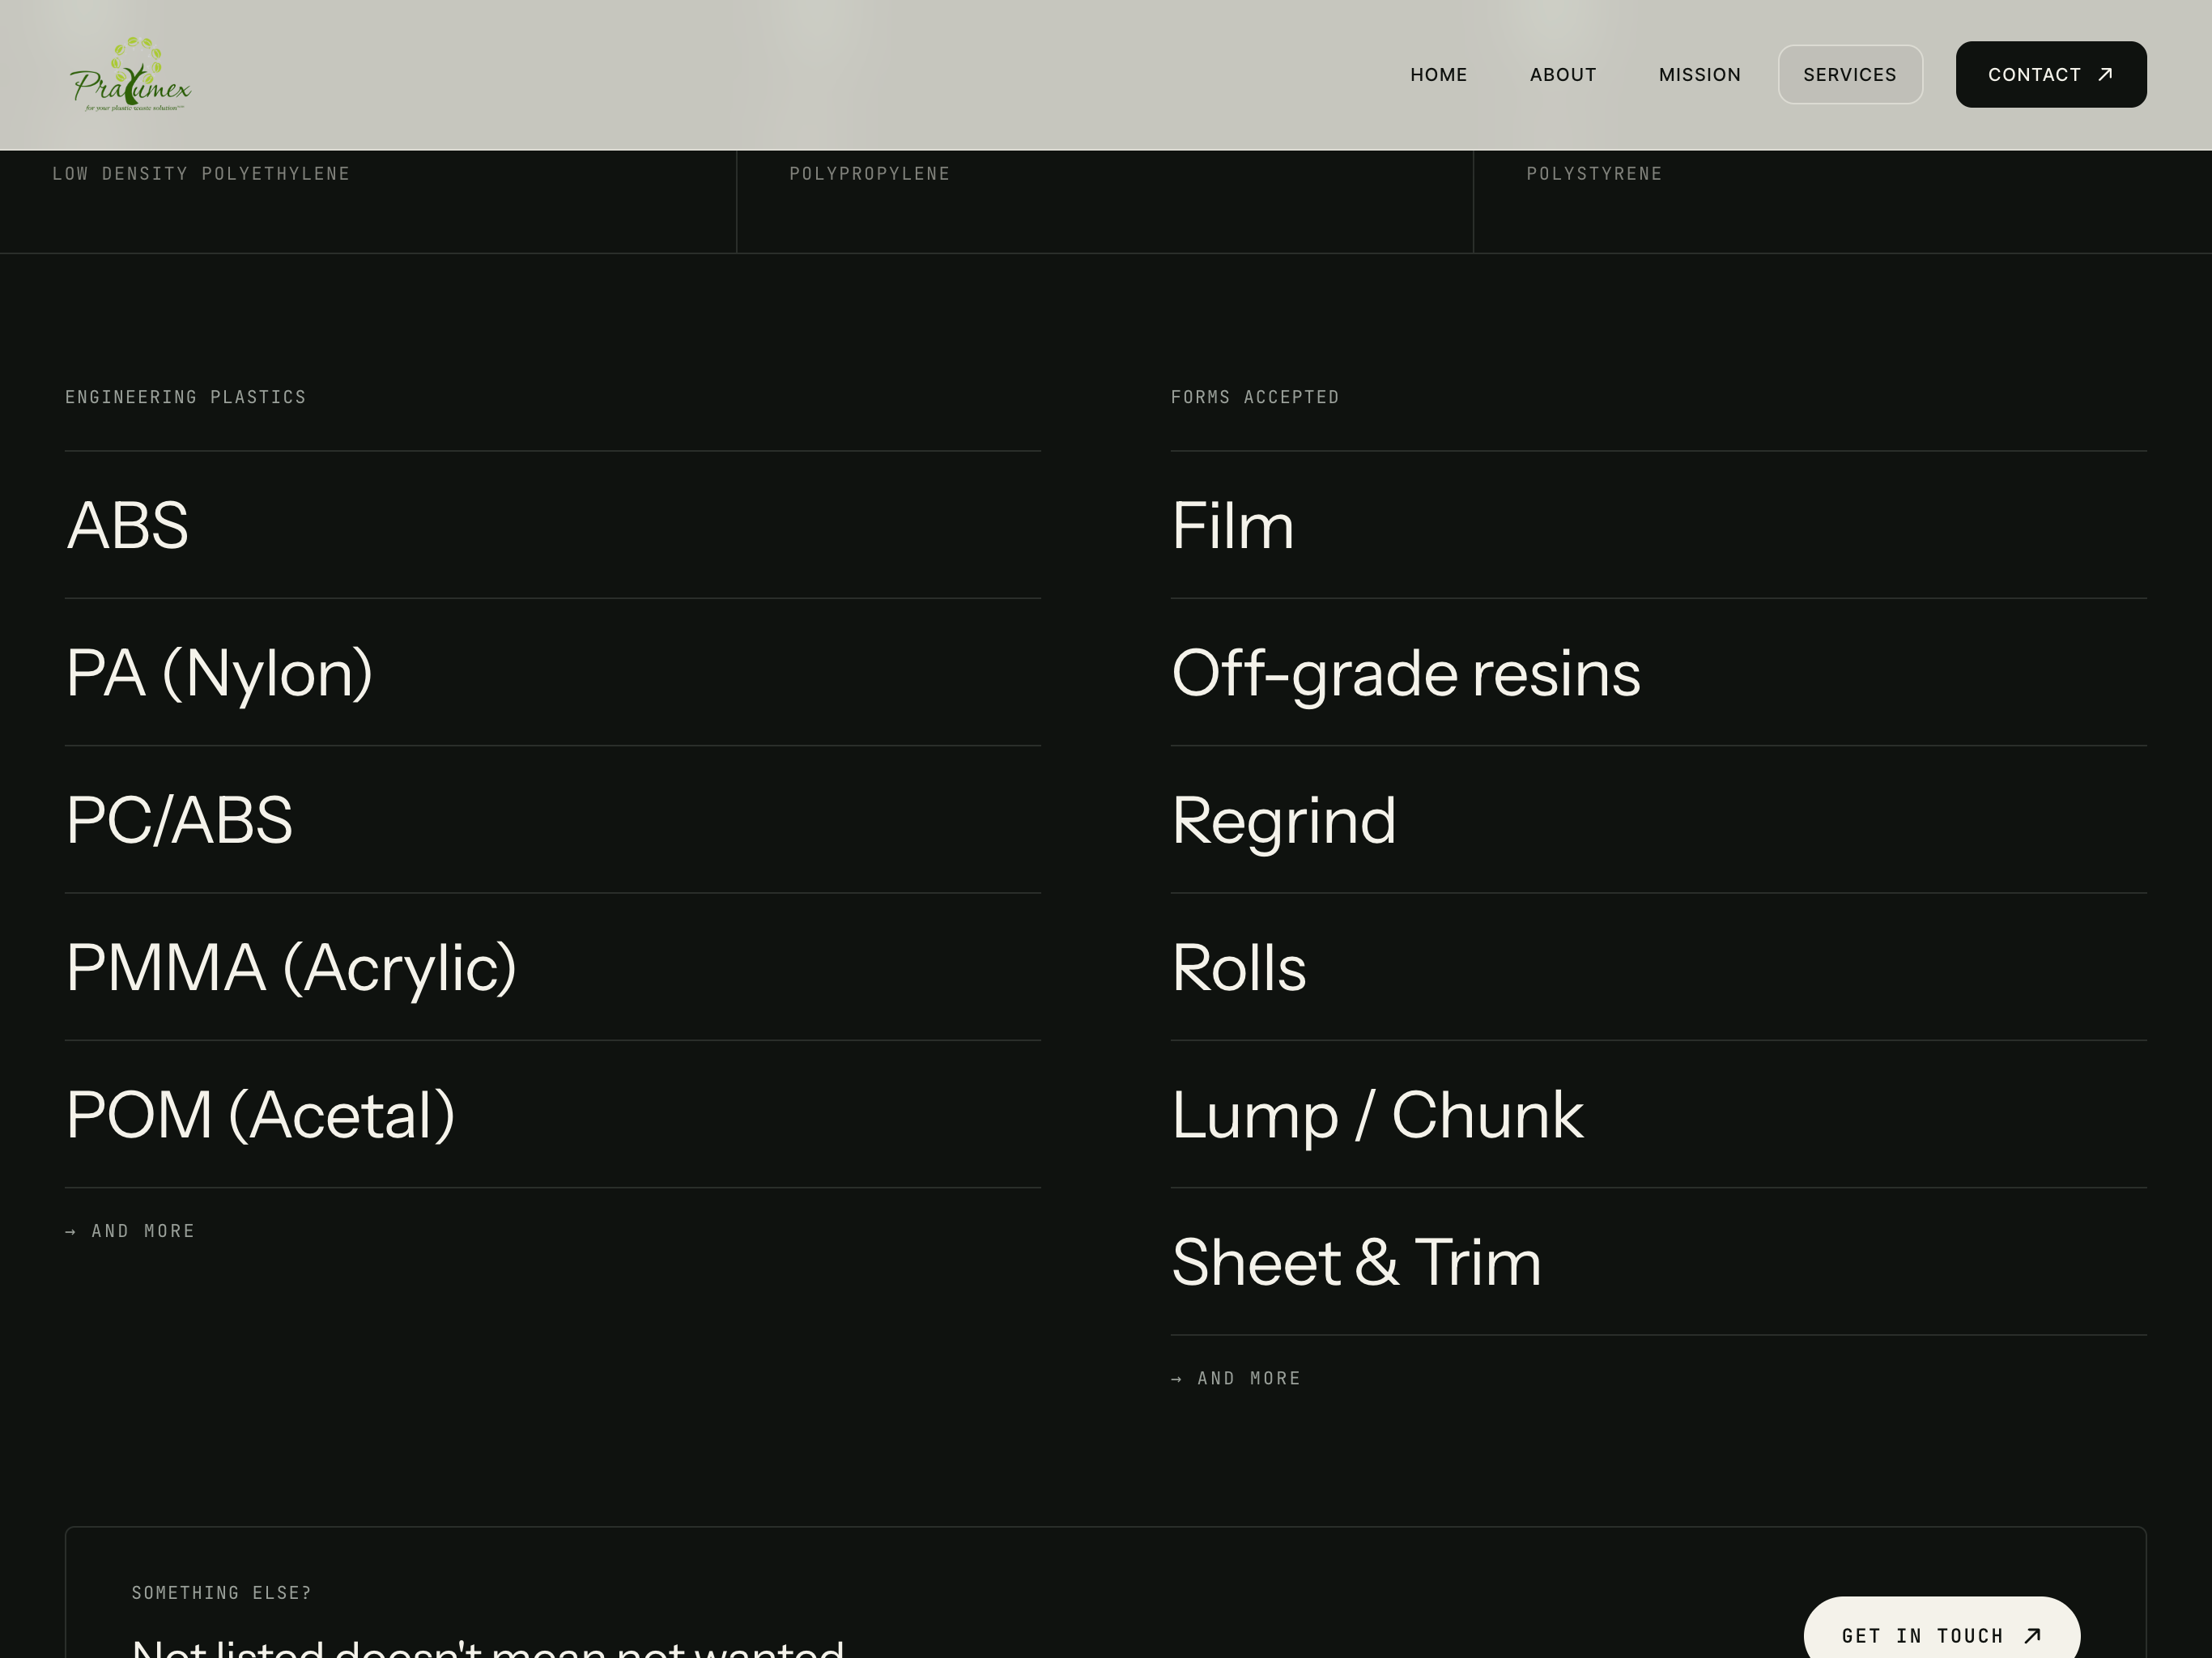
\includegraphics[width=\textwidth,height=0.46\textheight,keepaspectratio]{images/pralumex-website/beta/17.png}\\[4pt]
            
\includegraphics[width=\textwidth,height=0.46\textheight,keepaspectratio]{images/pralumex-website/beta/18.png}
            \end{figure}\clearpage
            \begin{figure}[H]\centering
            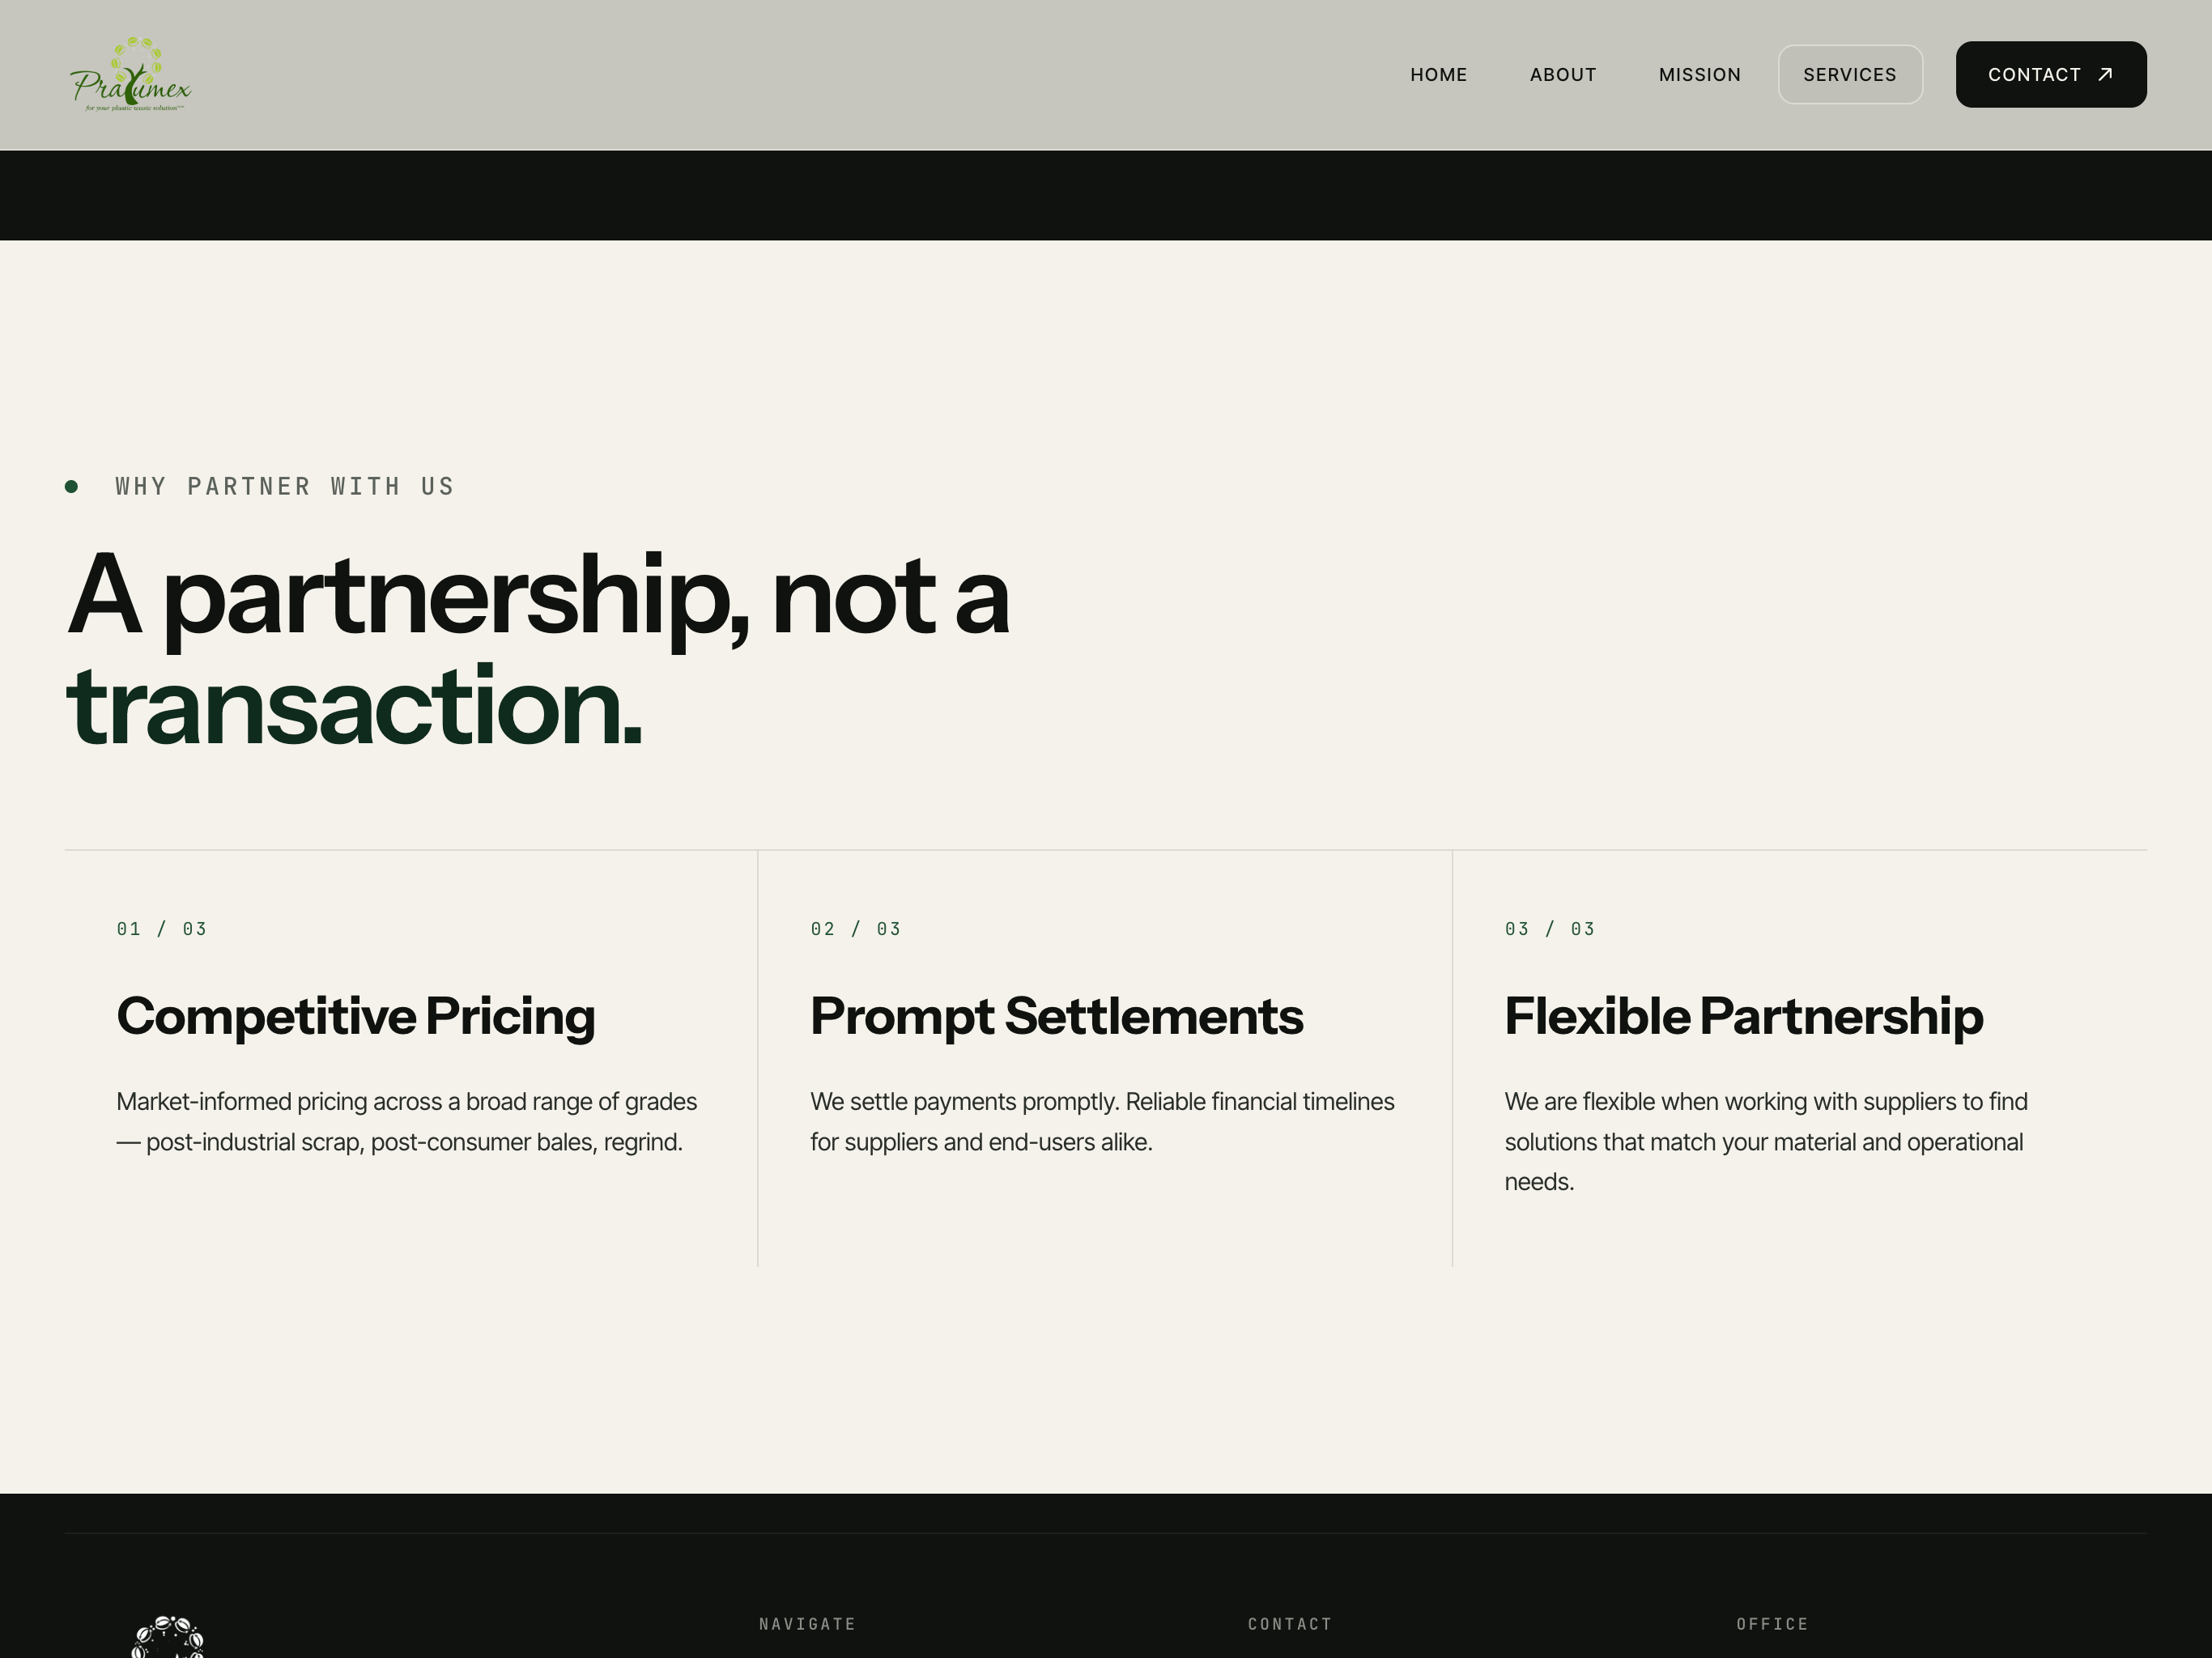
\includegraphics[width=\textwidth,height=0.46\textheight,keepaspectratio]{images/pralumex-website/beta/19.png}\\[4pt]
            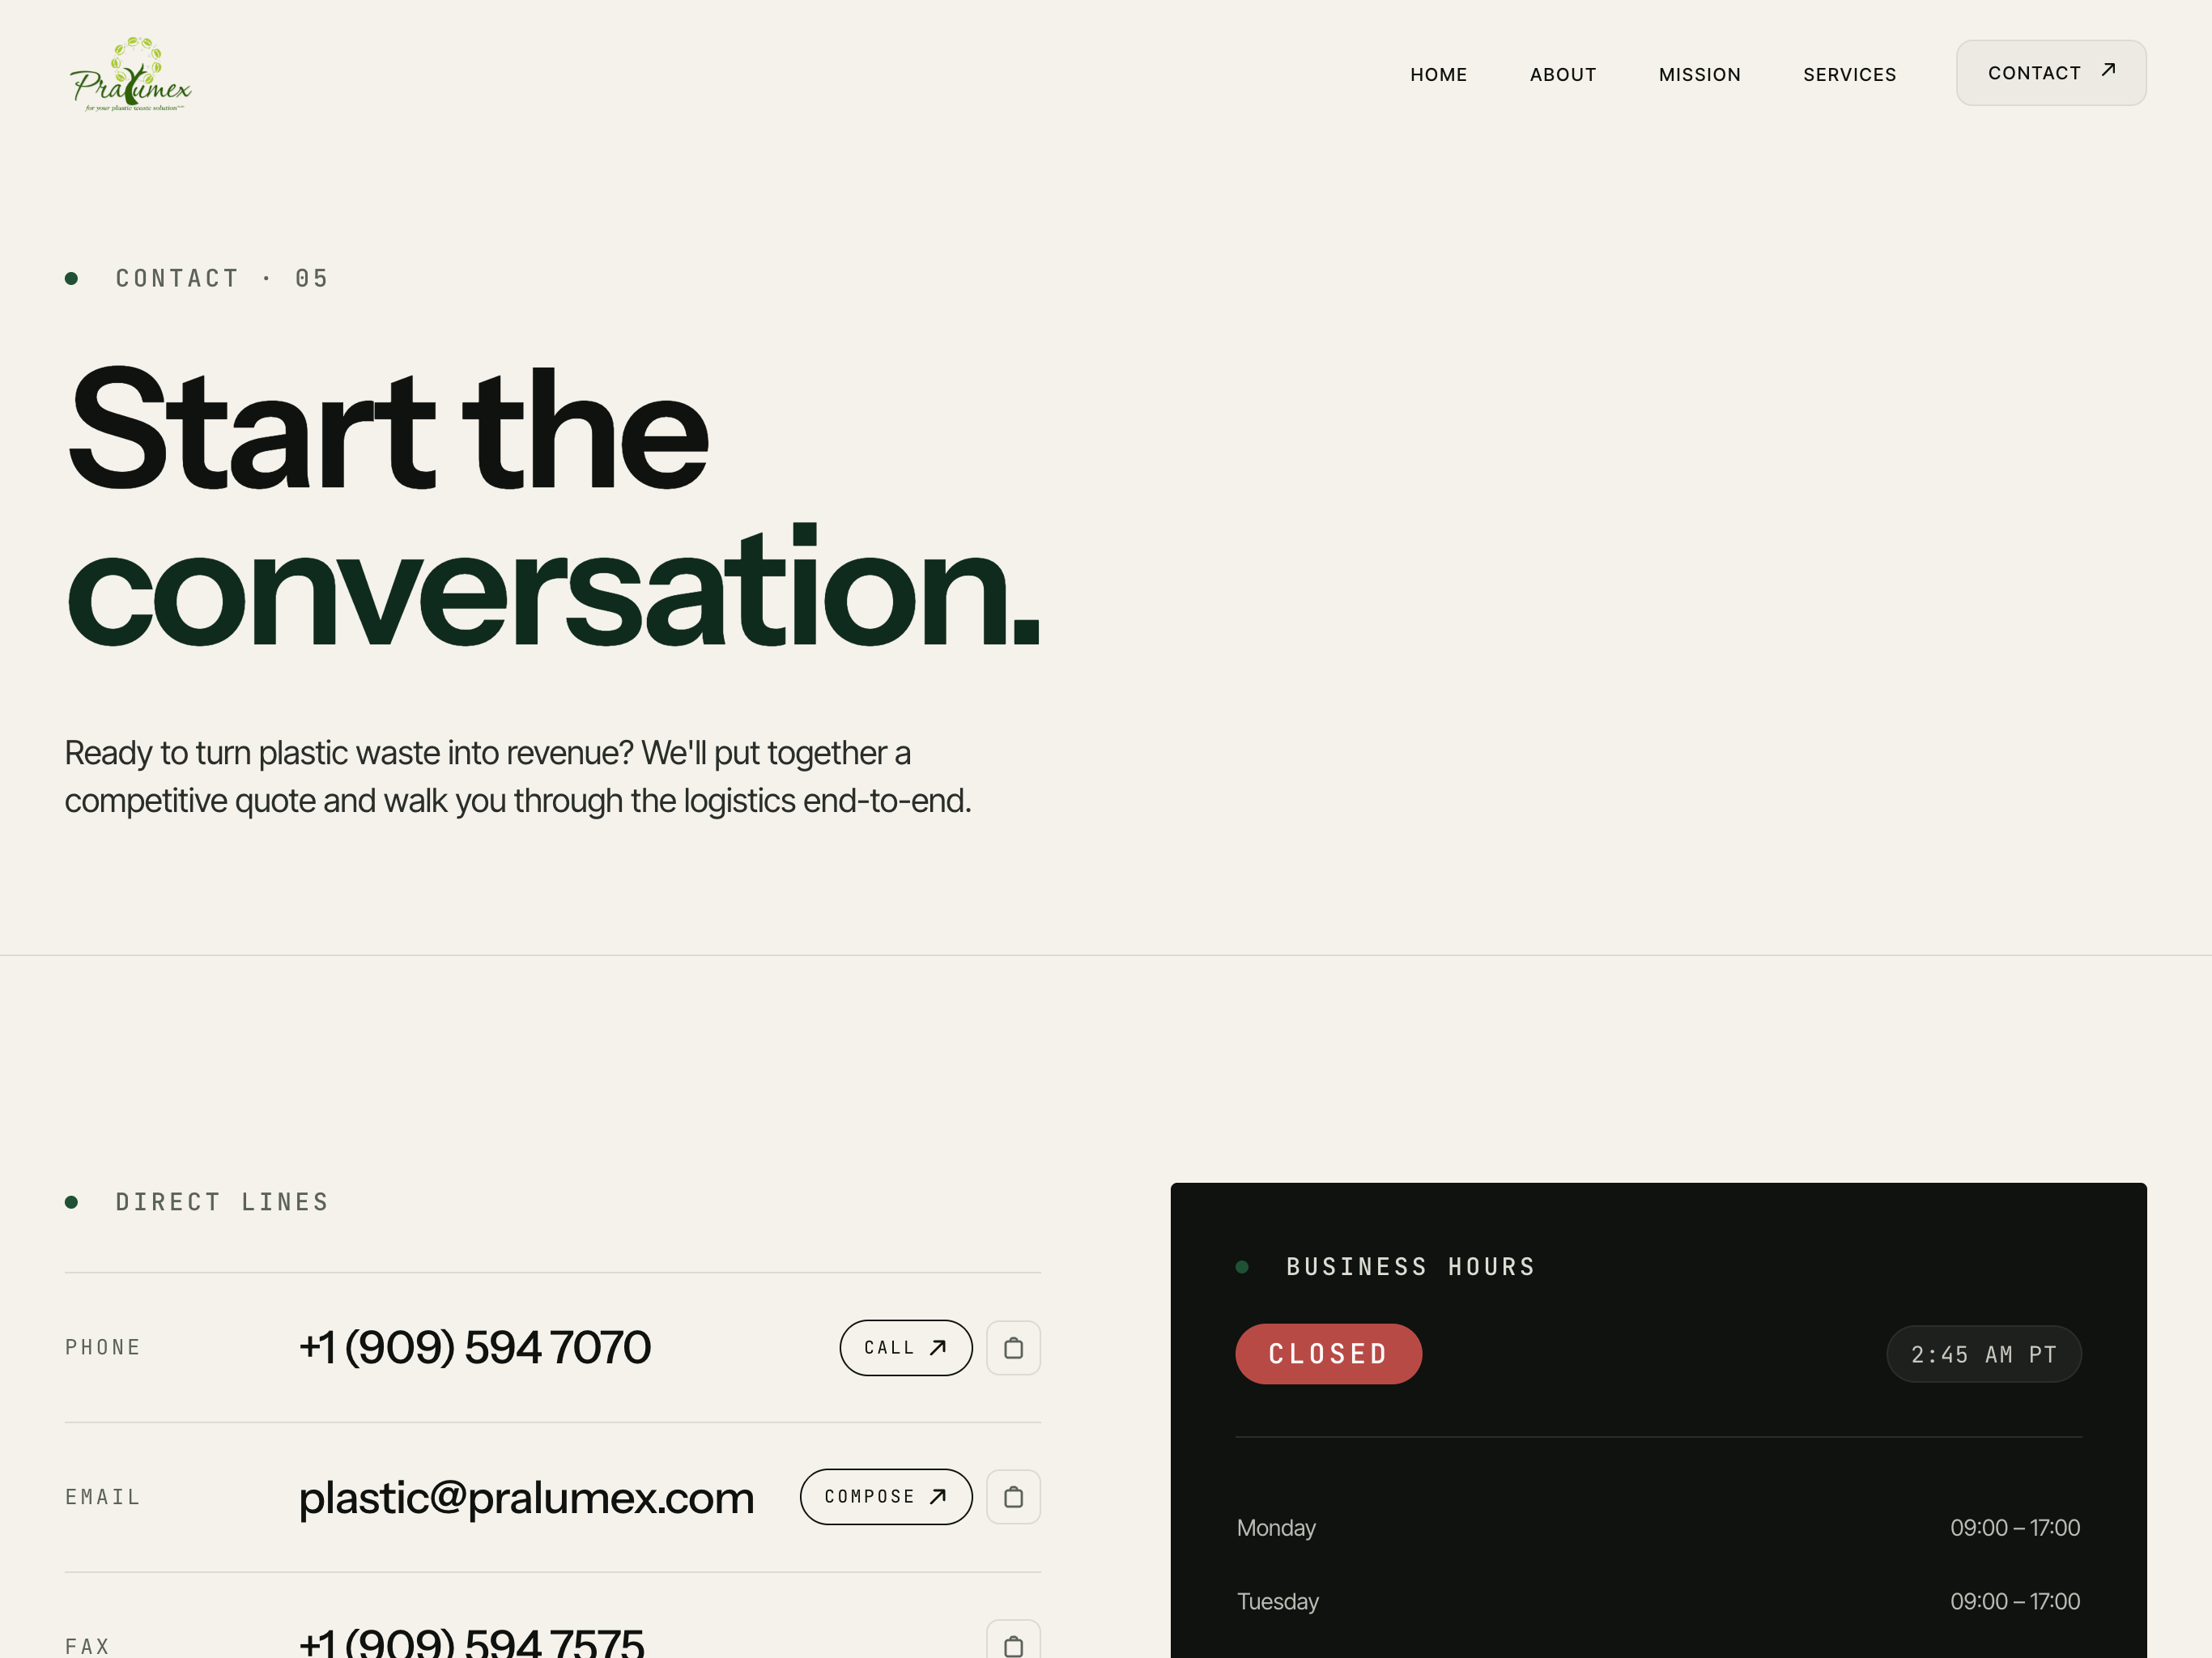
\includegraphics[width=\textwidth,height=0.46\textheight,keepaspectratio]{images/pralumex-website/beta/20.png}
            \end{figure}\clearpage
            \begin{figure}[H]\centering
            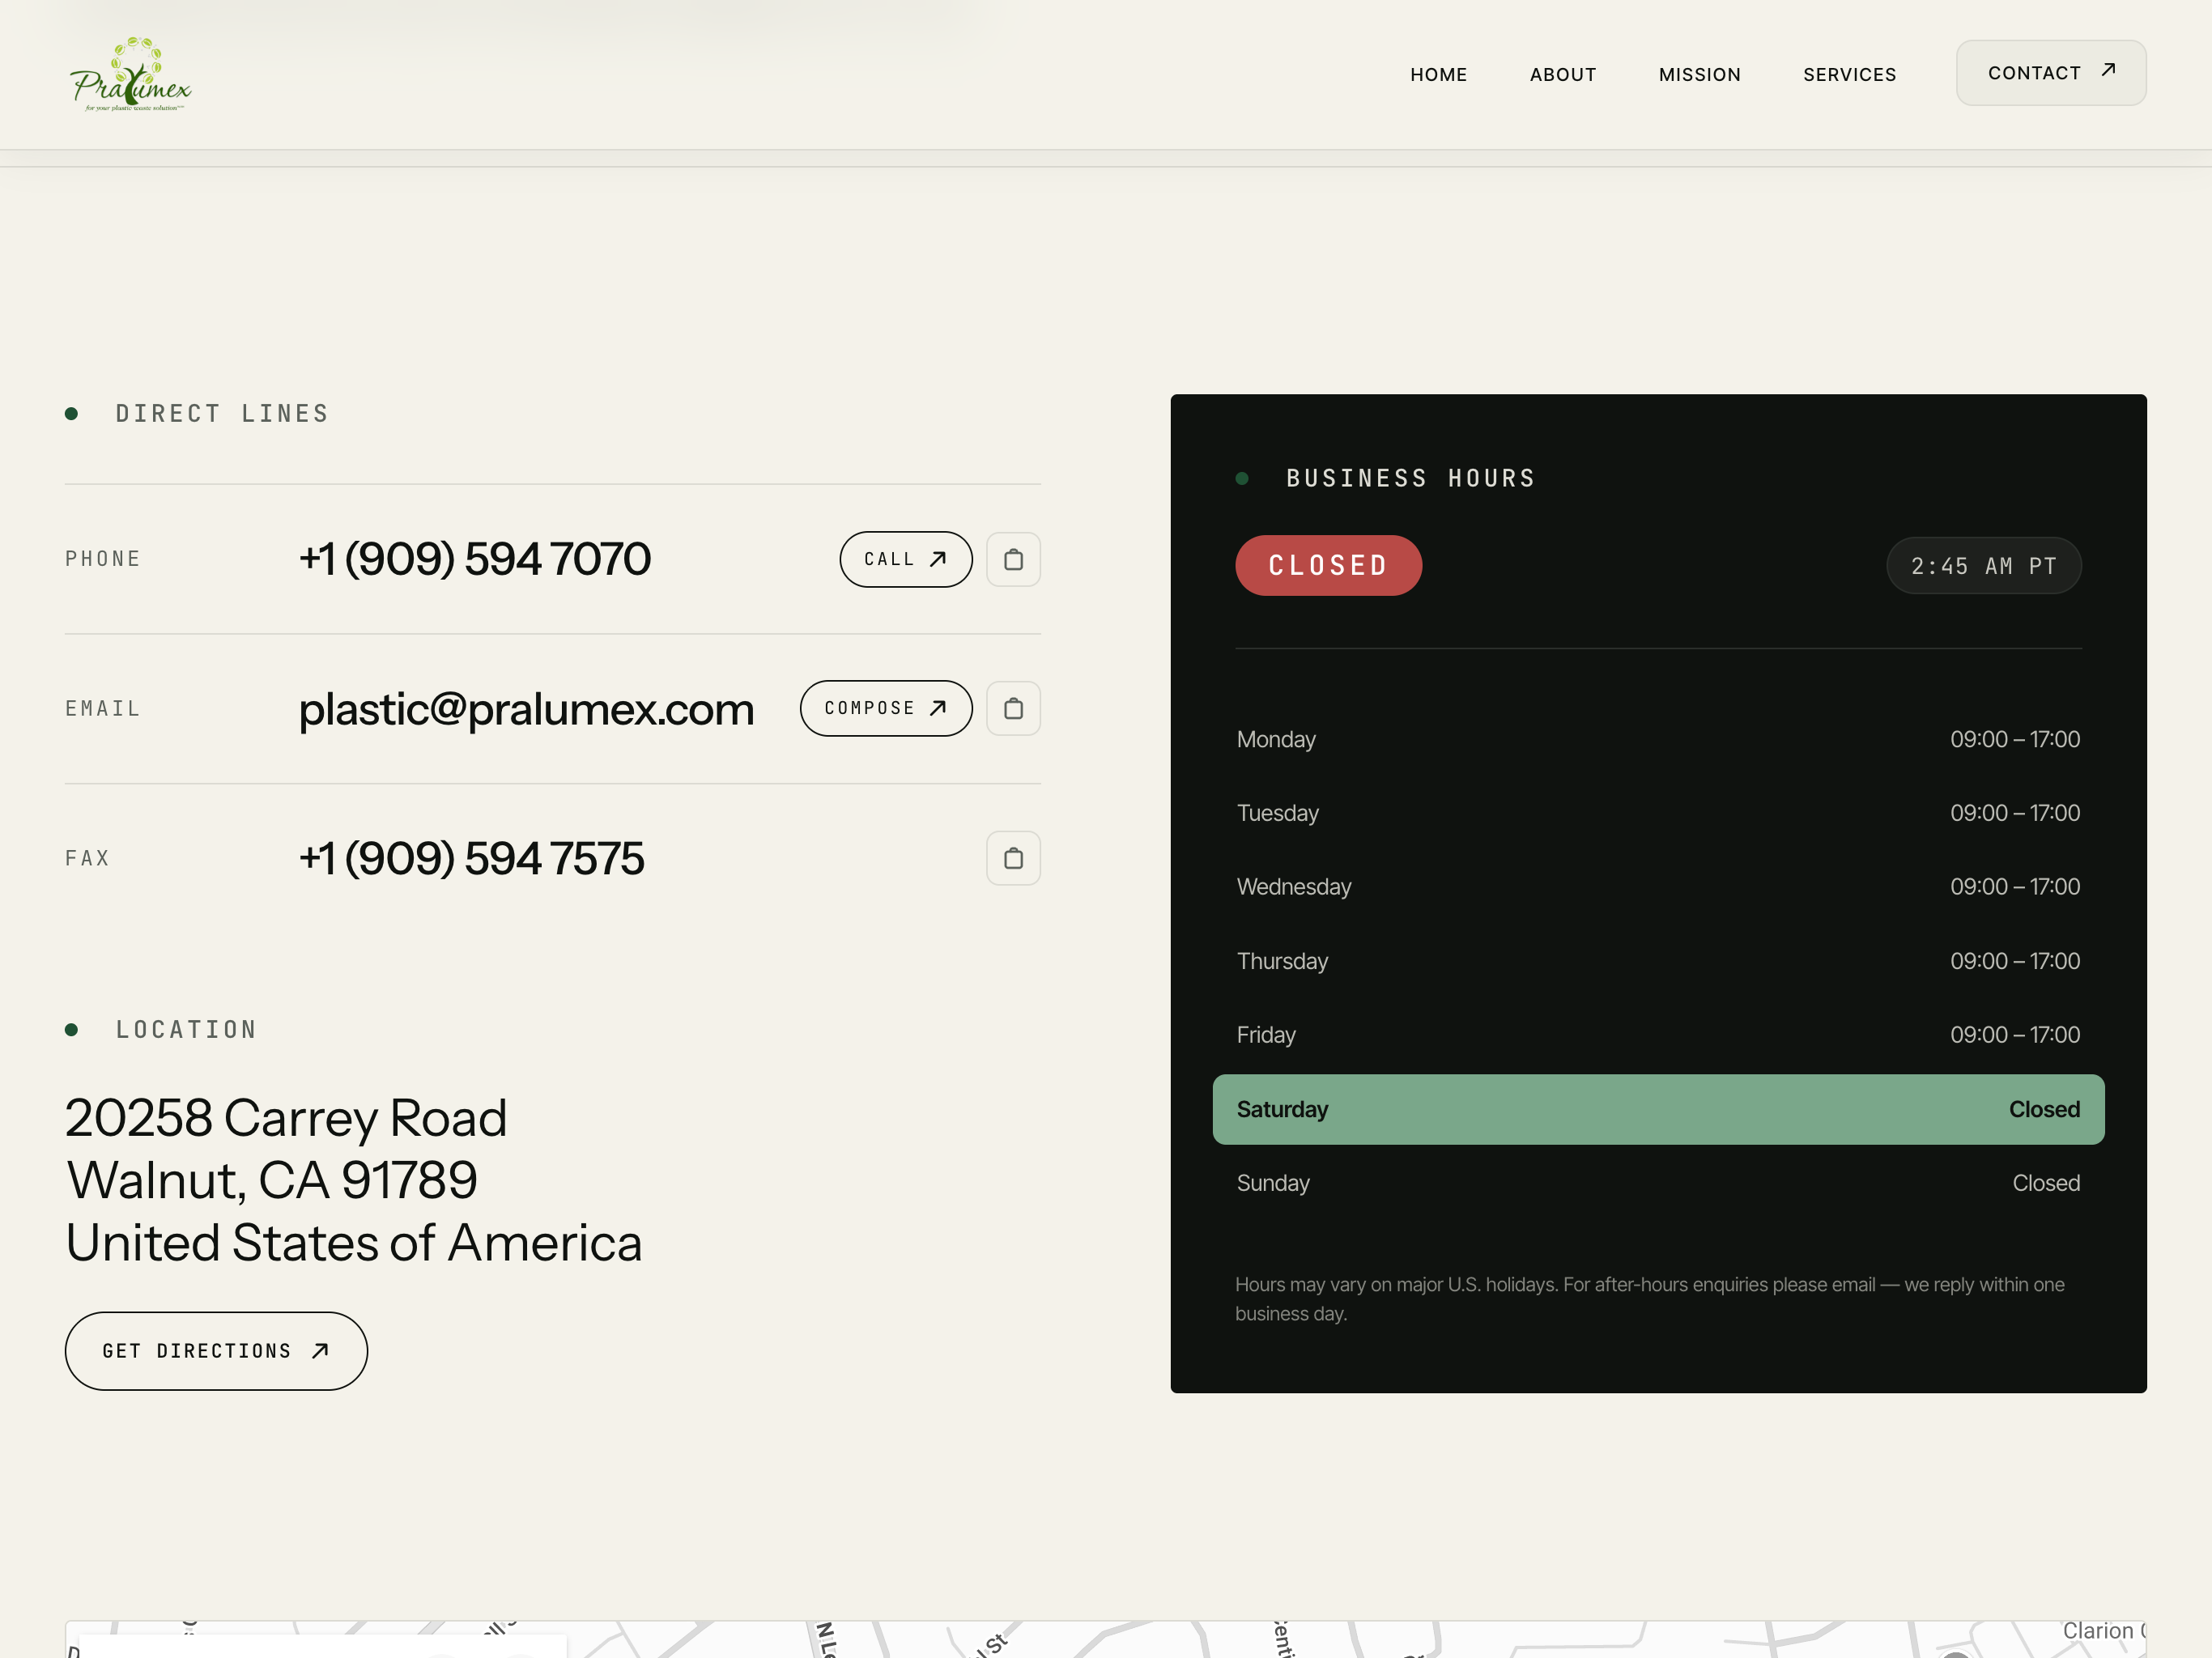
\includegraphics[width=\textwidth,height=0.46\textheight,keepaspectratio]{images/pralumex-website/beta/21.png}\\[4pt]
            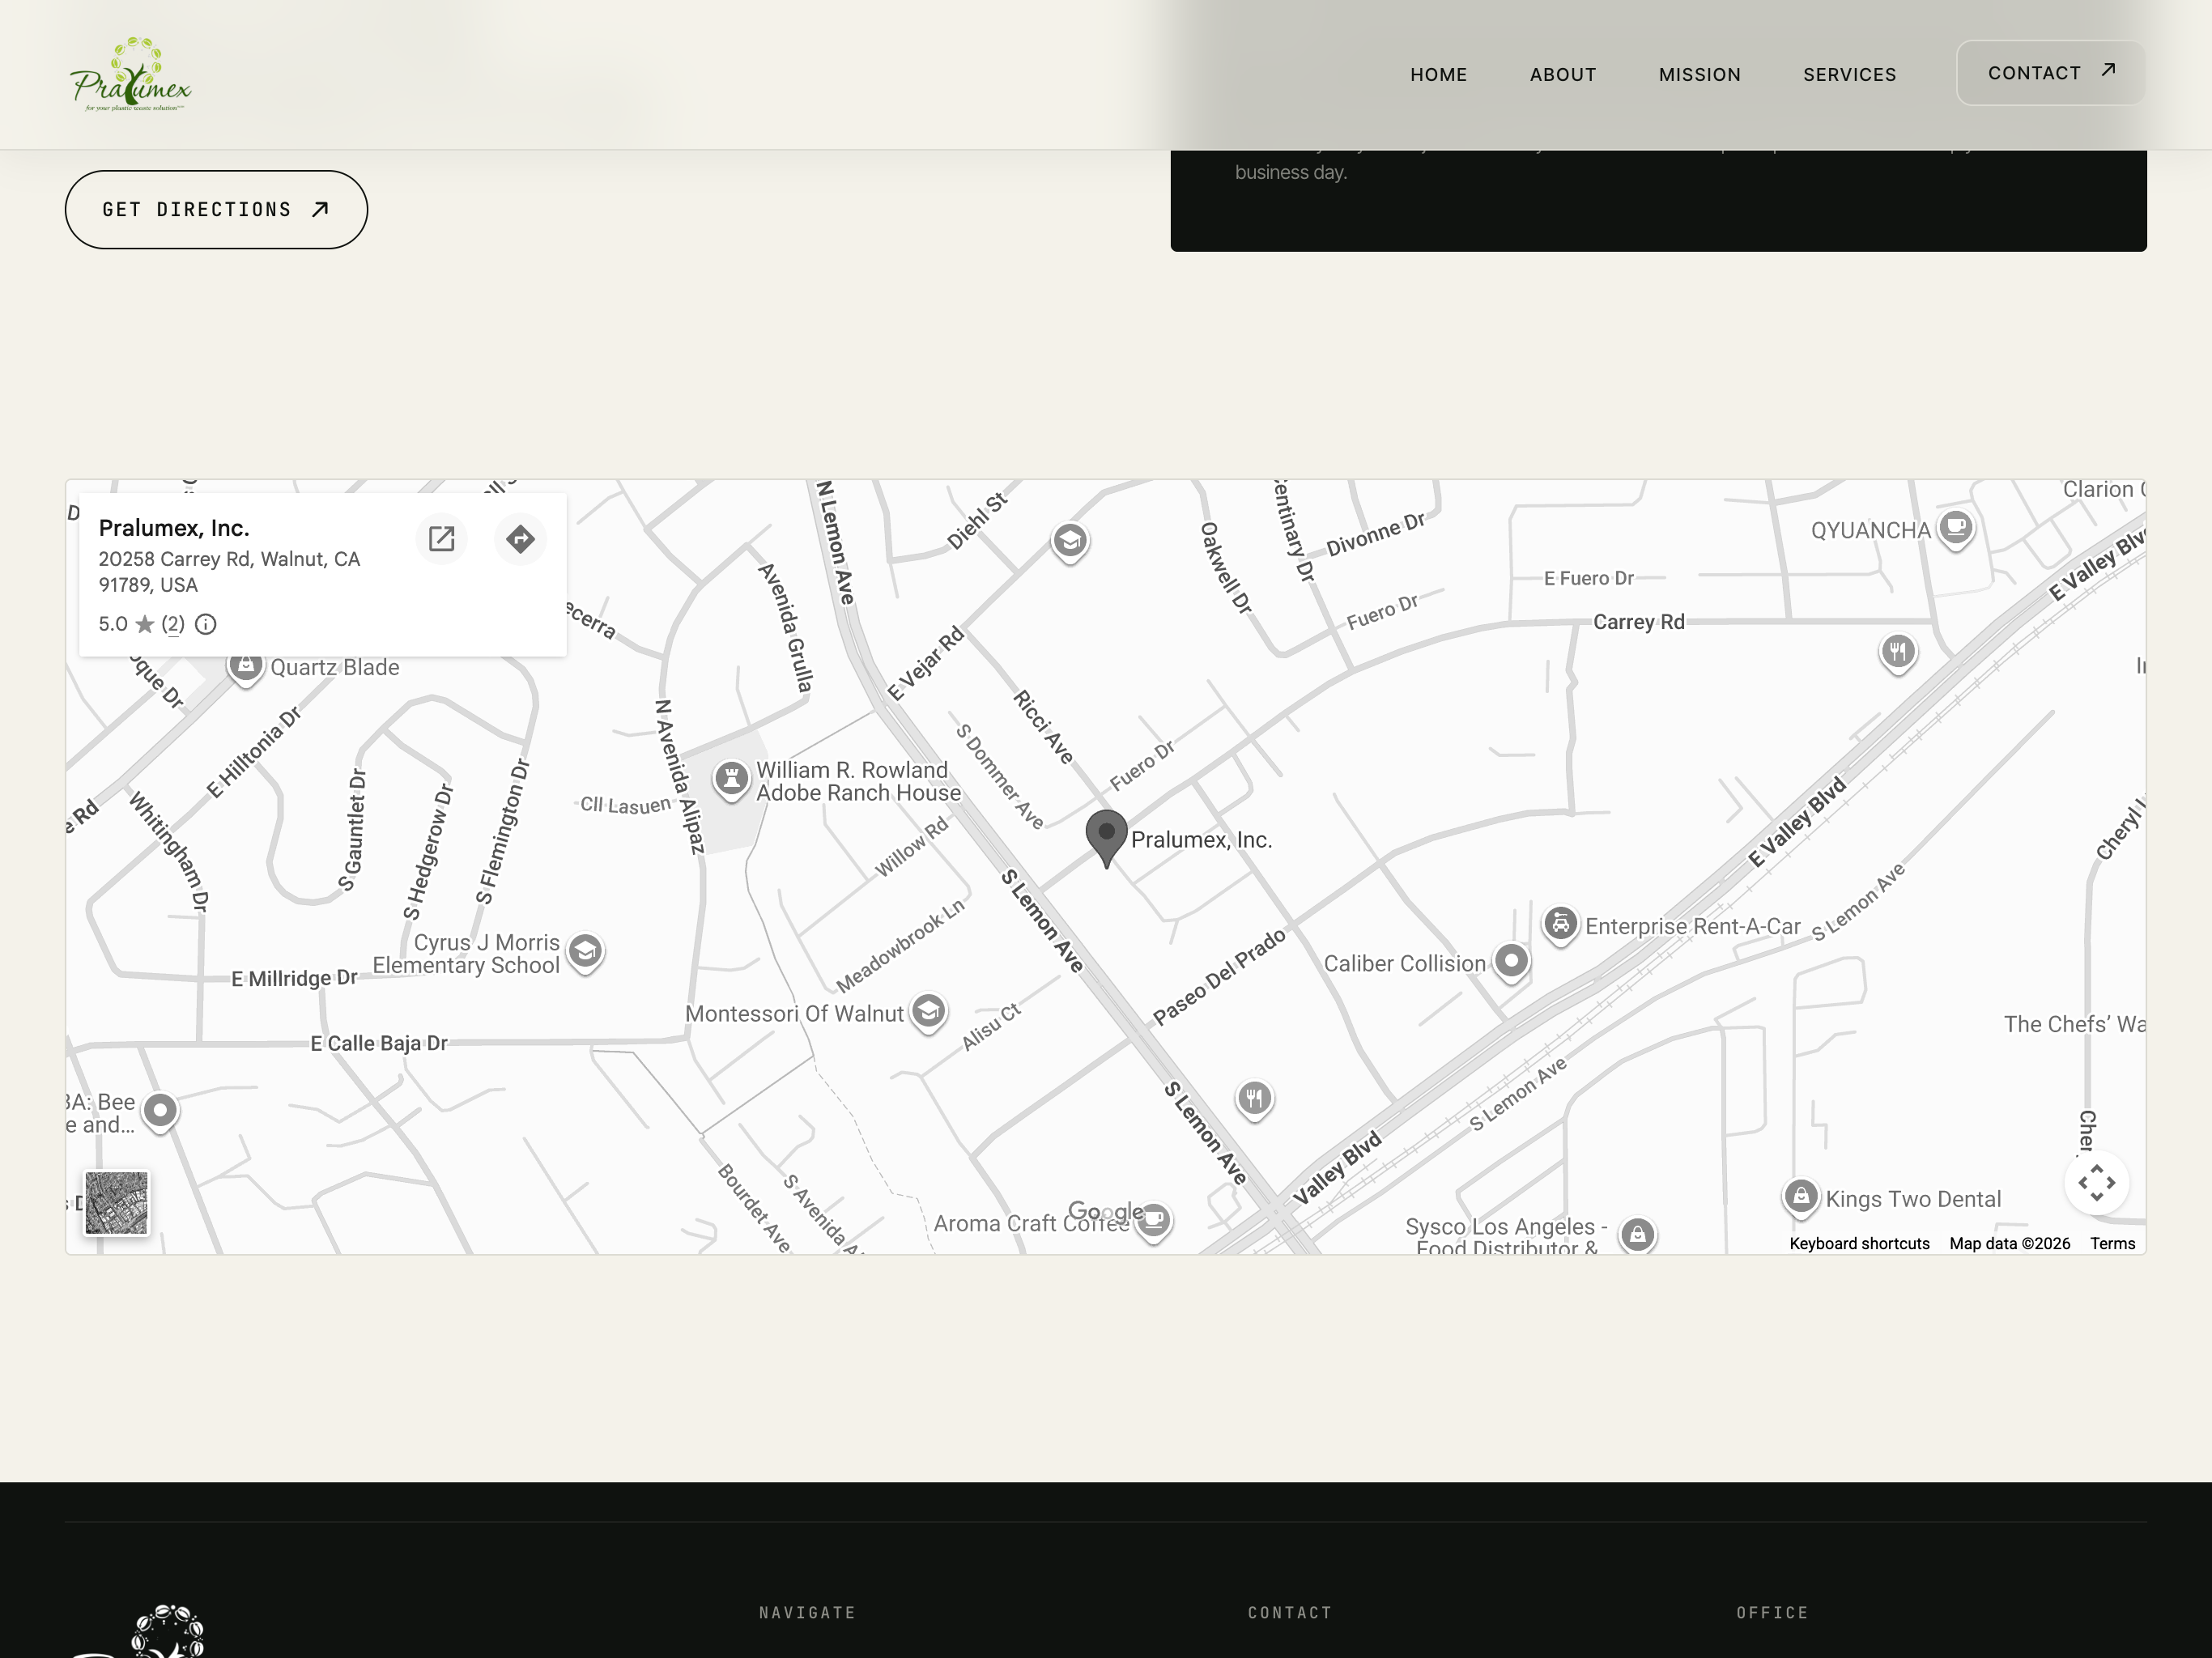
\includegraphics[width=\textwidth,height=0.46\textheight,keepaspectratio]{images/pralumex-website/beta/22.png}
            \end{figure}\clearpage

        \newpage
        \phantomsection\label{appendix:f}
        \subsection{Appendix F: Frontend Design \& UI/UX Videos \& Sources}

        % Links or screenshots of videos and resources used

\end{document}
